\documentclass[12pt]{article}
\usepackage[latin1]{inputenc}
\usepackage[headings]{fullpage}
\usepackage[noweb]{ocamlweb}
\pagestyle{headings}
\usepackage{url} \usepackage{graphicx}
\begin{document}
%%%%%%%%%%%%%%%%%%%%%%%%%%%%%%%%%%%%%%%%%%%%%%%%%%%%%%%%%%%%%%%%%
%% This file has been automatically generated with the command
%% ocamlweb -p \usepackage{url} \usepackage{graphicx} --noweb intro.tex ../pidgin.ml gen.tex ../gen.ml list2.tex ../list2.ml word.tex ../word.ml zipper.tex ../zipper.ml bintree.tex ../bintree.ml trie.tex ../trie.ml ascii.tex ../ascii.ml lexicon.tex ../lexicon.ml make_lex.tex ../make_lex.ml share.tex ../share.mli ../share.ml mini.tex ../mini.ml dagify.tex ../dagify.ml ../make_english_lexicon.ml english.tex ../zen_lexer.ml ../transducer.ml ../latin.ml french.tex ../make_french_lexicon.ml sanskrit.tex tertree.tex ../tertree.ml ../minitertree.ml deco.tex ../deco.ml lexmap.tex ../lexmap.ml minimap.tex ../minimap.mli ../minimap.ml unglue.tex ../unglue.ml ../unglue_test.ml coroutines.tex intro_aum0.tex ../aum0.mli react0.tex ../react0.ml aumt.tex ../aumt.mli reactt.tex ../reactt.ml regular.tex ../regular.ml linking.tex ../sanskrit_engine.ml conclusion.tex biblio.tex -o zen.tex 
%%%%%%%%%%%%%%%%%%%%%%%%%%%%%%%%%%%%%%%%%%%%%%%%%%%%%%%%%%%%%%%%%
%\documentclass[11pt]{article}
%\pagestyle{plain}

\def\lbr{\langle} %<
\def\rbr{\rangle} %>
\def\lsq{[} %[
\def\rsq{]} %]
\def\R{{\cal R}} % script R
\def\otrema{\"o} % otrema necessary for balance of "..." in comments.
\def\skip{\vspace{10pt}}

%\def\url{}

%\begin{document}
\begin{center}
\vspace*{24pt}
{\Large The Zen Computational Linguistics Toolkit}\\[10pt]
{\Large Version 3.2}\\[15pt]
{November 24th, 2013}\\[15pt]
{\large G\'erard Huet}\\[10pt]
{\large Copyright \copyright ~2002-2013 INRIA}\\[20pt]
\end{center}

\tableofcontents

\begin{abstract}
We present in this document a few fundamental structures useful for
computational linguistics. 

The central structure is that of lexical tree, or {\sl trie}.
A crucial observation is that a trie is isomorphic to the state space
of a deterministic acyclic automaton. More complex finite-state
automata and transducers, deterministic or not, and cyclic or
not, may be represented as tries decorated by extra information. Thus we
obtain a family of structures underlying lexicon-directed linguistic
processes.

First we describe plain tries, which are adequate to represent lexicon indexes.
Then we describe decorated tries, or {\sl decos}, which are appropriate to
represent symbol tables, and dictionaries associating with the lexicon
grammatical or other informations. We then describe how to represent
maps and more generally invertible relations between lexicons. We call these
structures lexical maps or {\sl lexmaps}. Lexmaps are appropriate for instance
to associate inflected forms to lexicon stems and roots, using morphological
operations. Such lexmaps are invertible in the sense that we may retrieve
from the lexmap entry of a inflected form the stems and operations from which
it may be obtained. Finally we show how lexicon directed transducers may
be represented using tries decorated with choice points. Such transducers
are useful to describe segmentation and taggings processes.

All data structures and algorithms are described
in a computational metalanguage called \verb:Pidgin ML:. \verb:Pidgin ML: is a 
publication language for the ML family of programming languages. All the
algorithms described here could be described as well in Standard ML
or in Objective CAML, to cite two popular ML implementations, or in the
lazy functional language Haskell. They could also be described in a 
programming language such as LISP or Scheme, but the strong typing discipline
of ML, supporting polymorphism and modules, is an insurance that computations
cannot corrupt data structures and lead to run-type errors. 
An initial chapter of these notes gives a quick overview of \verb:Pidgin ML:. 

The resulting design may be considered as the reference implementation of a Free 
Computational Linguistics Toolkit. It may turn useful as an ``off the shelf''
toolkit for simple operations on linguistics material. Due to its
lightweight approach we shall talk of the Zen CL Toolkit. 

This toolkit was abstracted from the Sanskrit ML Library, which constitutes
its first large-scale application. Thus some of this material already
appeared in the documentation of the Sanskrit Segmenter algorithm,
which solves Sandhi Analysis \cite{2004-Huet-1}.
%The Sanskrit Library Documentation, a companion to this document,
%is available at \url{http://pauillac.inria.fr/~huet/SKT/DOC/doc.ps} under
%format postscript, \verb|doc.pdf| under format pdf, 
%and \verb|doc.html| under format html.

This document was automatically generated from the code of the toolkit
using the Ocamlweb package of Jean-Christophe Filli\^atre,
with the Latex package, in the literate programming style pioneered by
Don Knuth. 
%The Html version uses the Hevea Tex-to-Html translator of Luc Maranget.

\end{abstract}

\part{Dictionaries}

\section{Pidgin ML}

We shall use as {\sl meta language} for the description of our algorithms
a pidgin version of the functional language ML 
\cite{ML-LCF,MLer,paulson,caml}. 
Readers familiar with ML
may skip this section, which gives a crash
overview of its syntax and semantics.

\typeout{OcamlWeb file Pidgin.ml}
\ocwmodule{Pidgin}
\label{../pidgin.ml:0}%
The core language has types, values, and exceptions. 
Thus, \ocwbegindcode{}1\ocwenddcode{} is a value of predefined type \ocwbegindcode{}\ocwbt{int}\ocwenddcode{}, whereas 
\ocwbegindcode{}\ocwstring{"CL"}\ocwenddcode{} is a \ocwbegindcode{}\ocwbt{string}\ocwenddcode{}. 
Pairs of values inhabit the corresponding product type. Thus:
\ocwbegindcode{}$(1,$\ocwstring{"CL"}$)~:~($\ocwbt{int}~$\times{}~$\ocwbt{string}$)$\ocwenddcode{}. 
Recursive type declarations create new types,
whose values are inductively built from the associated constructors. 
Thus the Boolean type could be declared
as a sum by: 
\ocweol
\label{../pidgin.ml:1092}%
\medskip
\ocwbegincode{}\ocwindent{0.00em}
\ocwkw{type}~\ocwbt{bool}~=~$[\ocwupperid{True}~\mid{}~\ocwupperid{False}];$\medskip

\ocwendcode{}\ocwindent{0.00em}
Parametric types give rise to polymorphism.
Thus if \ocwbegindcode{}$\ocwlowerid{x}$\ocwenddcode{} is of type \ocwbegindcode{}$\ocwlowerid{t}$\ocwenddcode{} and \ocwbegindcode{}$\ocwlowerid{l}$\ocwenddcode{} is of type 
\ocwbegindcode{}$($\ocwbt{list}~$\ocwlowerid{t})$\ocwenddcode{}, we construct the list adding \ocwbegindcode{}$\ocwlowerid{x}$\ocwenddcode{} to \ocwbegindcode{}$\ocwlowerid{l}$\ocwenddcode{}
as \ocwbegindcode{}[$\ocwlowerid{x}~::~\ocwlowerid{l}]$\ocwenddcode{}. The empty list is \ocwbegindcode{}$[\,]$\ocwenddcode{}, of (polymorphic) type
\ocwbegindcode{}$($\ocwbt{list}~$\alpha{})$\ocwenddcode{}. Although the language is strongly typed, explicit type
specification is rarely needed from the designer, since principal types
may be inferred mechanically.

The language is functional in the sense that functions are first class
objects. Thus the doubling integer function may be written as
\ocwbegindcode{}\ocwkw{fun}~$\ocwlowerid{x}~\rightarrow{}~\ocwlowerid{x}+\ocwlowerid{x}$\ocwenddcode{}, and it has type \ocwbegindcode{}\ocwbt{int}~$\rightarrow{}~$\ocwbt{int}\ocwenddcode{}. It may be associated
to the name \ocwbegindcode{}$\ocwlowerid{double}$\ocwenddcode{} by declaring: 
\ocweol
\label{../pidgin.ml:1737}%
\medskip
\ocwbegincode{}\ocwindent{0.00em}
$\ocwlowerid{value}~\ocwlowerid{double}~=~$\ocwkw{fun}~$\ocwlowerid{x}~\rightarrow{}~\ocwlowerid{x}+\ocwlowerid{x};$\medskip

\ocwendcode{}\ocwindent{0.00em}
Equivalently we could write: 
\ocweol
\label{../pidgin.ml:1802}%
\medskip
\ocwbegincode{}\ocwindent{0.00em}
$\ocwlowerid{value}~\ocwlowerid{double}~\ocwlowerid{x}~=~\ocwlowerid{x}+\ocwlowerid{x};$\medskip

\ocwendcode{}\ocwindent{0.00em}
Its application to value \ocwbegindcode{}$\ocwlowerid{n}$\ocwenddcode{}
is written as \ocwbegindcode{}$(\ocwlowerid{double}~\ocwlowerid{n})$\ocwenddcode{} or even \ocwbegindcode{}$\ocwlowerid{double}~\ocwlowerid{n}$\ocwenddcode{} when there is no
ambiguity. Application associates to the left, and thus \ocwbegindcode{}$\ocwlowerid{f}~\ocwlowerid{x}~\ocwlowerid{y}$\ocwenddcode{} stands
for \ocwbegindcode{}$((\ocwlowerid{f}~\ocwlowerid{x})~\ocwlowerid{y})$\ocwenddcode{}. 
Recursive functional values are declared with the keyword \ocwbegindcode{}\ocwkw{rec}\ocwenddcode{}.
Thus we may define factorial as: 
\ocweol
\label{../pidgin.ml:2111}%
\medskip
\ocwbegincode{}\ocwindent{0.00em}
$\ocwlowerid{value}~$\ocwkw{rec}~$\ocwlowerid{fact}~\ocwlowerid{n}~=~$\ocwkw{if}~$\ocwlowerid{n}=0~$\ocwkw{then}~1~\ocwkw{else}~$\ocwlowerid{n}\times{}(\ocwlowerid{fact}~(\ocwlowerid{n}-1));$\medskip

\ocwendcode{}\ocwindent{0.00em}
Functions may be defined by pattern matching. Thus the first projection of
pairs could be defined by: 
\ocweol
\label{../pidgin.ml:2274}%
\medskip
\ocwbegincode{}\ocwindent{0.00em}
$\ocwlowerid{value}~\ocwlowerid{fst}~=~$\ocwkw{fun}~$[~(\ocwlowerid{x},\ocwlowerid{y})~\rightarrow{}~\ocwlowerid{x}~];$\medskip

\ocwendcode{}\ocwindent{0.00em}
or equivalently (since there is only one pattern in this case) by: 
\ocweol
\label{../pidgin.ml:2380}%
\medskip
\ocwbegincode{}\ocwindent{0.00em}
$\ocwlowerid{value}~\ocwlowerid{fst}~(\ocwlowerid{x},\ocwlowerid{y})~=~\ocwlowerid{x};$\medskip

\ocwendcode{}\ocwindent{0.00em}
Pattern-matching is also usable in \ocwbegindcode{}\ocwkw{match}\ocwenddcode{} expressions which generalize
case analysis,
such as: \ocwbegindcode{}\ocwkw{match}~$\ocwlowerid{l}~$\ocwkw{with}~[~$[\,]~\rightarrow{}~\ocwupperid{True}~\mid{}~\ocwlowerid{\_}~\rightarrow{}~\ocwupperid{False}~]$\ocwenddcode{}, which
tests whether list \ocwbegindcode{}$\ocwlowerid{l}$\ocwenddcode{} is empty, using underscore as catch-all
pattern.

Evaluation is strict, which means that \ocwbegindcode{}$\ocwlowerid{x}$\ocwenddcode{} is evaluated before
\ocwbegindcode{}$\ocwlowerid{f}$\ocwenddcode{} in the evaluation of \ocwbegindcode{}$(\ocwlowerid{f}~\ocwlowerid{x})$\ocwenddcode{}. The \ocwbegindcode{}\ocwkw{let}\ocwenddcode{} expressions allow the
sharing of sub-computations. Thus
\ocwbegindcode{}\ocwkw{let}~$\ocwlowerid{x}~=~\ocwlowerid{fact}~10~$\ocwkw{in}~$\ocwlowerid{x}+\ocwlowerid{x}$\ocwenddcode{} will compute \ocwbegindcode{}$\ocwlowerid{fact}~10$\ocwenddcode{} first, 
and only once. 
An equivalent postfix \ocwbegindcode{}$\ocwlowerid{where}$\ocwenddcode{} notation may be used as well. Thus
the conditional expression \ocwbegindcode{}\ocwkw{if}~$\ocwlowerid{b}~$\ocwkw{then}~$\ocwlowerid{e1}~$\ocwkw{else}~$\ocwlowerid{e2}$\ocwenddcode{} is equivalent to: 
\ocweol
\ocwindent{0.00em}
\ocwbegindcode{}~$\ocwlowerid{choose}~\ocwlowerid{b}~\ocwlowerid{where}~\ocwlowerid{choose}~=~$\ocwkw{fun}~[~$\ocwupperid{True}~\rightarrow{}~\ocwlowerid{e1}~\mid{}~\ocwupperid{False}~\rightarrow{}~\ocwlowerid{e2}];~$\ocwenddcode{} 
\ocweol
\ocwindent{0.00em}
Exceptions are declared with the type of their parameters, like in: 
\ocweol
\label{../pidgin.ml:3138}%
\medskip
\ocwbegincode{}\ocwindent{0.00em}
\ocwkw{exception}~$\ocwupperid{Failure}~$\ocwkw{of}~\ocwbt{string};\medskip

\ocwendcode{}\ocwindent{0.00em}
An exceptional value may be raised, like in:
\ocwbegindcode{}$\ocwlowerid{raise}~(\ocwupperid{Failure}~$\ocwstring{"div\ocwvspace{}0"}$)$\ocwenddcode{} and handled by a \ocwbegindcode{}\ocwkw{try}\ocwenddcode{} switch on
exception patterns, such as: 
\ocweol
\ocwindent{0.00em}
\ocwbegindcode{}~\ocwkw{try}~$\ocwlowerid{expression}~$\ocwkw{with}~[~$\ocwupperid{Failure}~\ocwlowerid{s}~\rightarrow{}~...~];~$\ocwenddcode{} 
\ocweol
\ocwindent{0.00em}
Other imperative constructs may be used, such as 
references, mutable arrays, while loops and I/O commands,
but we shall seldom need them.
%If \ocwbegindcode{}$\ocwlowerid{x}$\ocwenddcode{} has been declared as a \ocwbegindcode{}\ocwbt{ref}~\ocwbt{int}\ocwenddcode{}, it may be assigned
%by an instruction such as \ocwbegindcode{}$\ocwlowerid{x}.$\ocwkw{val}:=0\ocwenddcode{}. 
Sequences of instructions are
evaluated in left to right regime in \ocwbegindcode{}\ocwkw{do}\ocwenddcode{} expressions, such as:
\ocwbegindcode{}\ocwkw{do}~\{$\ocwlowerid{e1};~...~\ocwlowerid{en}\}$\ocwenddcode{}. 

ML is a {\sl modular} language,
in the sense that sequences of type, value
and exception declarations may be packed in a structural unit called a
\ocwbegindcode{}\ocwkw{module}\ocwenddcode{}, amenable to separate treatment. 
Modules have types themselves, called {\sl signatures}. Parametric
modules are called {\sl functors}. The algorithms presented in this paper
will use in essential ways 
this modularity structure, but the syntax ought to be self-evident.
Finally, comments are enclosed within starred parens like: 
\ocweol
\label{../pidgin.ml:4208}%
\medskip
\ocwbegincode{}\ocwindent{0.00em}
$\ocwlowerid{value}~\ocwlowerid{s}~=~$\ocwstring{"This\ocwvspace{}is\ocwvspace{}a\ocwvspace{}string"};~\ocwbc{} This is a comment \ocwec{}\medskip

\ocwendcode{}\ocwindent{0.00em}
Readers not acquainted with programming languages may think of ML
definitions as recursive
equations over inductively defined algebras. Most of them are simple
primitive recursive functionals. The more complex recursions of our
automata coroutines will be shown to be well-founded by 
a combination of lexicographic and multiset orderings.

Pidgin ML definitions may actually be directly executed as 
Objective Caml programs \cite{ocaml},
under the so-called revised syntax \cite{camlp4}. 
The following development may thus 
be used as the reference implementation of a core
computational linguistics platform, dealing with lexical, phonemic and
morphological aspects. 

\ocweol
\section{Basic Utilities} 

We present in this section some basic utilities libraries.

\subsection{Miscellaneous primitives} 

\typeout{OcamlWeb file Gen.ml}
\ocwmodule{Gen}
\label{../gen.ml:0}%
This module contains various utilities of general use. 
\ocweol
\label{../gen.ml:708}%
\medskip
\ocwbegincode{}\ocwindent{0.00em}
$\ocwlowerid{value}~\ocwlowerid{dirac}~\ocwlowerid{b}~=~$\ocwkw{if}~$\ocwlowerid{b}~$\ocwkw{then}~1~\ocwkw{else}~0\ocweol
\ocwindent{0.00em}
;\ocweol
\ocwindent{0.00em}
$\ocwlowerid{value}~\ocwlowerid{optional}~\ocwlowerid{f}~=~$\ocwkw{fun}~$[~\ocwupperid{None}~\rightarrow{}~()~\mid{}~\ocwupperid{Some}~\ocwlowerid{d}~\rightarrow{}~\ocwlowerid{f}~\ocwlowerid{d}~]$\ocweol
\ocwindent{0.00em}
;\ocweol
\ocwindent{0.00em}
$\ocwlowerid{value}~\ocwlowerid{active}~=~$\ocwkw{fun}~$[~\ocwupperid{None}~\rightarrow{}~\ocwupperid{False}~\mid{}~\ocwupperid{Some}~\ocwlowerid{\_}~\rightarrow{}~\ocwupperid{True}~]$\ocweol
\ocwindent{0.00em}
;\medskip

\ocwendcode{}\ocwindent{0.00em}
Dump value \ocwbegindcode{}$\ocwlowerid{v}$\ocwenddcode{} on \ocwbegindcode{}$\ocwlowerid{file}$\ocwenddcode{}. 
\ocweol
\label{../gen.ml:890}%
\medskip
\ocwbegincode{}\ocwindent{0.00em}
$\ocwlowerid{value}~\ocwlowerid{dump}~\ocwlowerid{v}~\ocwlowerid{file}~=~$\ocweol
\ocwindent{1.00em}
\ocwkw{let}~$\ocwlowerid{cho}~=~\ocwlowerid{open\_out}~\ocwlowerid{file}~$\ocwkw{in}~\ocwkw{do}~\{~$\ocwlowerid{output\_value}~\ocwlowerid{cho}~\ocwlowerid{v};~\ocwlowerid{close\_out}~\ocwlowerid{cho}~\}$\ocweol
\ocwindent{0.00em}
;\medskip

\ocwendcode{}\ocwindent{0.00em}
Retrieve value dumped on \ocwbegindcode{}$\ocwlowerid{file}$\ocwenddcode{}; its type should be given in a cast. 
\ocweol
\label{../gen.ml:1059}%
\medskip
\ocwbegincode{}\ocwindent{0.00em}
$\ocwlowerid{value}~\ocwlowerid{gobble}~\ocwlowerid{file}~=~$\ocweol
\ocwindent{1.00em}
\ocwkw{let}~$\ocwlowerid{chi}~=~\ocwlowerid{open\_in}~\ocwlowerid{file}~$\ocwkw{in}\ocweol
\ocwindent{1.00em}
\ocwkw{let}~$\ocwlowerid{v}~=~\ocwlowerid{input\_value}~\ocwlowerid{chi}~$\ocwkw{in}~\ocwkw{do}~\{~$\ocwlowerid{close\_in}~\ocwlowerid{chi};~\ocwlowerid{v}~\}$\ocweol
\ocwindent{0.00em}
;\medskip

\ocwendcode{}\ocwindent{0.00em}
UNIX touch. 
\ocweol
\label{../gen.ml:1181}%
\medskip
\ocwbegincode{}\ocwindent{0.00em}
$\ocwlowerid{value}~\ocwlowerid{touch}~\ocwlowerid{file}~=~\ocwlowerid{close\_out}~(\ocwlowerid{open\_out}~\ocwlowerid{file})$\ocweol
\ocwindent{0.00em}
;\medskip

\label{../gen.ml:1229}%
\ocwindent{0.00em}
$\ocwlowerid{value}~\ocwlowerid{notify\_error}~\ocwlowerid{message}~=~$\ocweol
\ocwindent{1.00em}
\ocwkw{do}~\{~$\ocwlowerid{output\_string}~\ocwlowerid{stderr}~\ocwlowerid{message};~\ocwlowerid{flush}~\ocwlowerid{stderr}~\}$\ocweol
\ocwindent{0.00em}
;\ocweol
\ocweol
\ocwendcode{}\subsection{List processing}

We shall use lists intensively. We assume the standard library 
\ocwbegincode{}$\ocwupperid{List}$\ocwendcode{}. %[List]

\typeout{OcamlWeb file List2.ml}
\ocwmodule{List2}
\label{../list2.ml:0}%
We complement \ocwbegindcode{}$\ocwupperid{List}$\ocwenddcode{} here with a few auxiliary list service functions. 
\ocweol
\ocwindent{0.00em}
\ocwbegindcode{}$\ocwlowerid{unstack}~\ocwlowerid{l}~\ocwlowerid{r}~=~(\ocwlowerid{rev}~\ocwlowerid{l})~@~\ocwlowerid{r}$\ocwenddcode{} 
\ocweol
\ocwindent{0.00em}
\ocwbegindcode{}$\ocwlowerid{unstack}~=~\ocwupperid{List}.\ocwlowerid{rev\_append}$\ocwenddcode{} 
\ocweol
\label{../list2.ml:794}%
\medskip
\ocwbegincode{}\ocwindent{0.00em}
$\ocwlowerid{value}~$\ocwkw{rec}~$\ocwlowerid{unstack}~\ocwlowerid{l1}~\ocwlowerid{l2}~=$\ocweol
\ocwindent{1.00em}
\ocwkw{match}~$\ocwlowerid{l1}~$\ocwkw{with}\ocweol
\ocwindent{1.00em}
$[~[\,]~\rightarrow{}~\ocwlowerid{l2}$\ocweol
\ocwindent{1.00em}
$\mid{}~[~\ocwlowerid{a}~::~\ocwlowerid{l}~]~\rightarrow{}~\ocwlowerid{unstack}~\ocwlowerid{l}~[~\ocwlowerid{a}~::~\ocwlowerid{l2}~]$\ocweol
\ocwindent{1.00em}
$]$\ocweol
\ocwindent{0.00em}
;\ocweol
\ocwindent{0.00em}
$\ocwlowerid{value}~\ocwlowerid{non\_empty}~=~$\ocwkw{fun}~$[~[\,]~\rightarrow{}~\ocwupperid{False}~\mid{}~\ocwlowerid{\_}~\rightarrow{}~\ocwupperid{True}~]$\ocweol
\ocwindent{0.00em}
;\medskip

\ocwendcode{}\ocwindent{0.00em}
Subtraction derivative. 
\ocweol
\ocwindent{0.00em}
\ocwbegindcode{}$\ocwlowerid{subtract}~:~$\ocwbt{list}~$\alpha{}~\rightarrow{}~$\ocwbt{list}~$\alpha{}~\rightarrow{}~$\ocwbt{option}~$($\ocwbt{list}~$\alpha{})$\ocwenddcode{}              
\ocweol
\ocwindent{0.00em}
\ocwbegindcode{}$\ocwlowerid{subtract}~[~\ocwlowerid{c1};~...~\ocwlowerid{cN}~][~\ocwlowerid{c1};~...~\ocwlowerid{cn}~]~=~\ocwupperid{Some}~[~\ocwlowerid{cn}+1;~...~\ocwlowerid{cN}~]$\ocwenddcode{}  
\ocweol
\ocwindent{0.00em}
otherwise returns \ocwbegindcode{}$\ocwupperid{None}$\ocwenddcode{}.                                         
\ocweol
\label{../list2.ml:1192}%
\medskip
\ocwbegincode{}\ocwindent{0.00em}
$\ocwlowerid{value}~$\ocwkw{rec}~$\ocwlowerid{subtract}~\ocwlowerid{input}~=~$\ocwkw{fun}\ocweol
\ocwindent{1.00em}
$[~[\,]~\rightarrow{}~\ocwupperid{Some}~\ocwlowerid{input}$\ocweol
\ocwindent{1.00em}
$\mid{}~[~\ocwlowerid{c}~::~\ocwlowerid{r}~]~\rightarrow{}~$\ocwkw{match}~$\ocwlowerid{input}~$\ocwkw{with}~\ocweol
\ocwindent{2.50em}
$[~[~\ocwlowerid{c'}~::~\ocwlowerid{r'}~]~$\ocwkw{when}~$\ocwlowerid{c'}=\ocwlowerid{c}~\rightarrow{}~\ocwlowerid{subtract}~\ocwlowerid{r'}~\ocwlowerid{r}$\ocweol
\ocwindent{2.50em}
$\mid{}~\ocwlowerid{\_}~\rightarrow{}~\ocwupperid{None}$\ocweol
\ocwindent{2.50em}
$]$\ocweol
\ocwindent{1.00em}
$]$\ocweol
\ocwindent{0.00em}
;\medskip

\ocwendcode{}\ocwindent{0.00em}
Association lists. 
\ocweol
\ocwindent{0.00em}
The right way to program \ocwbegindcode{}$\ocwlowerid{assoc}$\ocwenddcode{}, without exceptions. 
\ocweol
\ocwindent{0.00em}
\ocwbegindcode{}$\ocwlowerid{ass}~:~\alpha{}~\rightarrow{}~$\ocwbt{list}~$(\alpha{}~\times{}~\beta{})~\rightarrow{}~$\ocwbt{option}~$\beta{}$\ocwenddcode{} 
\ocweol
\label{../list2.ml:1492}%
\medskip
\ocwbegincode{}\ocwindent{0.00em}
$\ocwlowerid{value}~\ocwlowerid{ass}~\ocwlowerid{x}~=~\ocwlowerid{ass\_rec}~$\ocweol
\ocwindent{1.00em}
$\ocwlowerid{where}~$\ocwkw{rec}~$\ocwlowerid{ass\_rec}~=~$\ocwkw{fun}~\ocweol
\ocwindent{1.00em}
$[~[~(\ocwlowerid{a},\ocwlowerid{u})~::~\ocwlowerid{rest}~]~\rightarrow{}~$\ocwkw{if}~$\ocwlowerid{a}=\ocwlowerid{x}~$\ocwkw{then}~$\ocwupperid{Some}~\ocwlowerid{u}~$\ocwkw{else}~$\ocwlowerid{ass\_rec}~\ocwlowerid{rest}$\ocweol
\ocwindent{1.00em}
$\mid{}~[\,]~\rightarrow{}~\ocwupperid{None}$\ocweol
\ocwindent{1.00em}
$]$\ocweol
\ocwindent{0.00em}
;\medskip

\ocwendcode{}\ocwindent{0.00em}
Set operations with lists. 
\ocweol
\label{../list2.ml:1660}%
\medskip
\ocwbegincode{}\ocwindent{0.00em}
\ocwkw{exception}~$\ocwupperid{Twice\_the\_same\_value}~$\ocweol
\ocwindent{0.00em}
;\ocweol
\ocwindent{0.00em}
$\ocwlowerid{value}~\ocwlowerid{union1}~\ocwlowerid{e}~\ocwlowerid{l}~=~$\ocweol
\ocwindent{1.00em}
\ocwkw{if}~$\ocwupperid{List.}\ocwlowerid{mem}~\ocwlowerid{e}~\ocwlowerid{l}~$\ocwkw{then}~$\ocwlowerid{l}~$\ocwkw{else}~$[~\ocwlowerid{e}~::~\ocwlowerid{l}~]$\ocweol
\ocwindent{0.00em}
;\medskip

\ocwendcode{}\ocwindent{0.00em}
Used in ZEN/Lexmap. 
\ocweol
\label{../list2.ml:1784}%
\medskip
\ocwbegincode{}\ocwindent{0.00em}
$\ocwlowerid{value}~\ocwlowerid{union2}~\ocwlowerid{e}~\ocwlowerid{l}~=~$\ocweol
\ocwindent{1.50em}
\ocwkw{if}~$\ocwupperid{List.}\ocwlowerid{mem}~\ocwlowerid{e}~\ocwlowerid{l}~$\ocwkw{then}~$(\ocwlowerid{raise}~\ocwupperid{Twice\_the\_same\_value})~$\ocwkw{else}~$[~\ocwlowerid{e}~::~\ocwlowerid{l}~]$\ocweol
\ocwindent{0.00em}
;\medskip

\ocwendcode{}\ocwindent{0.00em}
Terminal recursive union of finite sets represented as as lists - does not 
   respect the order of elements in \ocwbegindcode{}$\ocwlowerid{l1}$\ocwenddcode{}: \ocwbegindcode{}$\ocwlowerid{union\_f}~[~1;~2~]~[\,]~=~[~2;~1~]$\ocwenddcode{}    
\ocweol
\label{../list2.ml:2036}%
\medskip
\ocwbegincode{}\ocwindent{0.00em}
$\ocwlowerid{value}~$\ocwkw{rec}~$\ocwlowerid{union\_f}~\ocwlowerid{l1}~\ocwlowerid{l2}~=~$\ocweol
\ocwindent{1.00em}
\ocwkw{match}~$\ocwlowerid{l1}~$\ocwkw{with}\ocweol
\ocwindent{2.00em}
$[~[\,]~\rightarrow{}~\ocwlowerid{l2}$\ocweol
\ocwindent{2.00em}
$\mid{}~[~\ocwlowerid{e}~::~\ocwlowerid{l}~]~\rightarrow{}~\ocwlowerid{union\_f}~\ocwlowerid{l}~(\ocwlowerid{union1}~\ocwlowerid{e}~\ocwlowerid{l2})$\ocweol
\ocwindent{2.00em}
$]~$\ocweol
\ocwindent{0.00em}
;\medskip

\ocwendcode{}\ocwindent{0.00em}
Same, respecting the order: 
\ocweol
\label{../list2.ml:2182}%
\medskip
\ocwbegincode{}\ocwindent{0.00em}
$\ocwlowerid{value}~\ocwlowerid{union}~\ocwlowerid{l1}~\ocwlowerid{l2}~=~\ocwupperid{List.}\ocwlowerid{fold\_right}~\ocwlowerid{union1}~\ocwlowerid{l1}~\ocwlowerid{l2}$\ocweol
\ocwindent{0.00em}
;\ocweol
\ocwindent{0.00em}
$\ocwlowerid{value}~\ocwlowerid{set\_of}~\ocwlowerid{l}~=~$\ocwkw{let}~$\ocwlowerid{add}~\ocwlowerid{acc}~\ocwlowerid{x}~=~$\ocwkw{if}~$\ocwupperid{List.}\ocwlowerid{mem}~\ocwlowerid{x}~\ocwlowerid{acc}~$\ocwkw{then}~$\ocwlowerid{acc}~$\ocwkw{else}~$[~\ocwlowerid{x}~::~\ocwlowerid{acc}~]~$\ocwkw{in}\ocweol
\ocwindent{1.00em}
$\ocwupperid{List.}\ocwlowerid{fold\_left}~\ocwlowerid{add}~[\,]~\ocwlowerid{l}$\ocweol
\ocwindent{0.00em}
;\medskip

\ocwendcode{}\ocwindent{0.00em}
\ocwbegindcode{}$\ocwlowerid{last}~:~$\ocwbt{list}~$\alpha{}~\rightarrow{}~\alpha{}~$\ocwenddcode{} 
\ocweol
\label{../list2.ml:2415}%
\medskip
\ocwbegincode{}\ocwindent{0.00em}
$\ocwlowerid{value}~$\ocwkw{rec}~$\ocwlowerid{last}~=~$\ocwkw{fun}~\ocweol
\ocwindent{1.00em}
$[~[\,]~\rightarrow{}~\ocwlowerid{raise}~(\ocwupperid{Failure}~$\ocwstring{"last"}$)$\ocweol
\ocwindent{1.00em}
$\mid{}~[~\ocwlowerid{x}~]~\rightarrow{}~\ocwlowerid{x}$\ocweol
\ocwindent{1.00em}
$\mid{}~[~\ocwlowerid{\_}~::~\ocwlowerid{l}~]~\rightarrow{}~\ocwlowerid{last}~\ocwlowerid{l}$\ocweol
\ocwindent{1.00em}
$]$\ocweol
\ocwindent{0.00em}
;\medskip

\ocwendcode{}\ocwindent{0.00em}
\ocwbegindcode{}$\ocwlowerid{truncate}~\ocwlowerid{n}~\ocwlowerid{l}$\ocwenddcode{} removes from \ocwbegindcode{}$\ocwlowerid{l}$\ocwenddcode{} its initial sublist of length \ocwbegindcode{}$\ocwlowerid{n}$\ocwenddcode{}. 
\ocweol
\ocwindent{0.00em}
\ocwbegindcode{}$\ocwlowerid{truncate}~:~$\ocwbt{int}~$\rightarrow{}~$\ocwbt{list}~$\alpha{}~\rightarrow{}~$\ocwbt{list}~$\alpha{}$\ocwenddcode{}                             
\ocweol
\label{../list2.ml:2736}%
\medskip
\ocwbegincode{}\ocwindent{0.00em}
$\ocwlowerid{value}~$\ocwkw{rec}~$\ocwlowerid{truncate}~\ocwlowerid{n}~\ocwlowerid{l}~=~$\ocweol
\ocwindent{1.00em}
\ocwkw{if}~$\ocwlowerid{n}=0~$\ocwkw{then}~$\ocwlowerid{l}~$\ocwkw{else}~\ocwkw{match}~$\ocwlowerid{l}~$\ocwkw{with}~\ocweol
\ocwindent{1.50em}
$[~[\,]~\rightarrow{}~\ocwlowerid{failwith}~$\ocwstring{"truncate"}~\ocweol
\ocwindent{1.50em}
$\mid{}~[~\ocwlowerid{\_}~::~\ocwlowerid{r}~]~\rightarrow{}~\ocwlowerid{truncate}~(\ocwlowerid{n}-1)~\ocwlowerid{r}$\ocweol
\ocwindent{1.50em}
$]$\ocweol
\ocwindent{0.00em}
;\ocweol
\ocwindent{0.00em}
\ocwkw{type}~$\ocwlowerid{ranked}~\alpha{}~=~$\ocwbt{list}~$($\ocwbt{int}~$\times{}~\alpha{})$\ocweol
\ocwindent{0.00em}
;\medskip

\ocwendcode{}\ocwindent{0.00em}
\ocwbegindcode{}$\ocwlowerid{zip}~\ocwlowerid{n}~\ocwlowerid{l}$\ocwenddcode{} assumes \ocwbegindcode{}$\ocwlowerid{l}$\ocwenddcode{} sorted in increasing order of ranks; it returns 
   a partition of \ocwbegindcode{}$\ocwlowerid{l}$\ocwenddcode{} as \ocwbegindcode{}$(\ocwlowerid{l1},\ocwlowerid{l2})$\ocwenddcode{} with \ocwbegindcode{}$\ocwlowerid{l1}$\ocwenddcode{} maximum such that ranks in \ocwbegindcode{}$\ocwlowerid{l1}$\ocwenddcode{}
   are  \ocwbegindcode{}$<~\ocwlowerid{n}$\ocwenddcode{}. \ocwbegindcode{}$\ocwlowerid{l1}$\ocwenddcode{} is reversed, i.e. we enforce the invariant:
   \ocwbegindcode{}$\ocwlowerid{zip}~\ocwlowerid{n}~\ocwlowerid{l}~=~(\ocwlowerid{l1},\ocwlowerid{l2})$\ocwenddcode{} such that \ocwbegindcode{}$\ocwlowerid{l}~=~\ocwlowerid{unstack}~\ocwlowerid{l1}~\ocwlowerid{l2}$\ocwenddcode{}.                      
\ocweol
\ocwindent{0.00em}
\ocwbegindcode{}$\ocwlowerid{zip}~:~$\ocwbt{int}~$\rightarrow{}~(\ocwlowerid{ranked}~\alpha{})~\rightarrow{}~((\ocwlowerid{ranked}~\alpha{})~\times{}~(\ocwlowerid{ranked}~\alpha{}))$\ocwenddcode{}               
\ocweol
\label{../list2.ml:3357}%
\medskip
\ocwbegincode{}\ocwindent{0.00em}
$\ocwlowerid{value}~\ocwlowerid{zip}~\ocwlowerid{n}~=~\ocwlowerid{zip\_rec}~[\,]~$\ocweol
\ocwindent{1.00em}
$\ocwlowerid{where}~$\ocwkw{rec}~$\ocwlowerid{zip\_rec}~\ocwlowerid{acc}~\ocwlowerid{l}~=~$\ocwkw{match}~$\ocwlowerid{l}~$\ocwkw{with}\ocweol
\ocwindent{1.00em}
$[~[\,]~\rightarrow{}~(\ocwlowerid{acc},[\,])$\ocweol
\ocwindent{1.00em}
$\mid{}~[~((\ocwlowerid{m},\ocwlowerid{\_})~$\ocwkw{as}~$\ocwlowerid{current})~::~\ocwlowerid{rest}~]~\rightarrow{}~$\ocweol
\ocwindent{3.00em}
\ocwkw{if}~$\ocwlowerid{m}<\ocwlowerid{n}~$\ocwkw{then}~$\ocwlowerid{zip\_rec}~[~\ocwlowerid{current}~::~\ocwlowerid{acc}~]~\ocwlowerid{rest}$\ocweol
\ocwindent{3.00em}
\ocwkw{else}~$(\ocwlowerid{acc},\ocwlowerid{l})$\ocweol
\ocwindent{1.00em}
$]$\ocweol
\ocwindent{0.00em}
;\medskip

\ocwendcode{}\ocwindent{0.00em}
Coercions between \ocwbegindcode{}\ocwbt{string}\ocwenddcode{} and \ocwbegindcode{}\ocwbt{list}~\ocwbt{char}\ocwenddcode{}. 
\ocweol
\ocwindent{0.00em}
\ocwbegindcode{}$\ocwlowerid{explode}~:~$\ocwbt{string}~$\rightarrow{}~$\ocwbt{list}~\ocwbt{char}\ocwenddcode{}             
\ocweol
\label{../list2.ml:3708}%
\medskip
\ocwbegincode{}\ocwindent{0.00em}
$\ocwlowerid{value}~\ocwlowerid{explode}~\ocwlowerid{s}~=$\ocweol
\ocwindent{1.00em}
\ocwkw{let}~\ocwkw{rec}~$\ocwlowerid{expl}~\ocwlowerid{i}~\ocwlowerid{accu}~=$\ocweol
\ocwindent{2.00em}
\ocwkw{if}~$\ocwlowerid{i}~<~0~$\ocwkw{then}~$\ocwlowerid{accu}~$\ocwkw{else}~$\ocwlowerid{expl}~(\ocwlowerid{i}~-~1)~[~\ocwlowerid{s}.[\ocwlowerid{i}]~::~\ocwlowerid{accu}~]~$\ocwkw{in}\ocweol
\ocwindent{1.00em}
$\ocwlowerid{expl}~(\ocwupperid{String.}\ocwlowerid{length}~\ocwlowerid{s}~-~1)~[\,]$\ocweol
\ocwindent{0.00em}
;\medskip

\ocwendcode{}\ocwindent{0.00em}
\ocwbegindcode{}$\ocwlowerid{implode}:~$\ocwbt{list}~\ocwbt{char}~$\rightarrow{}~$\ocwbt{string}\ocwenddcode{} 
\ocweol
\label{../list2.ml:3884}%
\medskip
\ocwbegincode{}\ocwindent{0.00em}
$\ocwlowerid{value}~\ocwlowerid{implode}~\ocwlowerid{l}~=$\ocweol
\ocwindent{1.00em}
\ocwkw{let}~$\ocwlowerid{result}~=~\ocwupperid{Bytes.}\ocwlowerid{create}~(\ocwupperid{List.}\ocwlowerid{length}~\ocwlowerid{l})~$\ocwkw{in}\ocweol
\ocwindent{1.00em}
\ocwkw{let}~\ocwkw{rec}~$\ocwlowerid{loop}~\ocwlowerid{i}~=~$\ocwkw{fun}\ocweol
\ocwindent{3.00em}
$[~[\,]~\rightarrow{}~\ocwlowerid{result}$\ocweol
\ocwindent{3.00em}
$\mid{}~[~\ocwlowerid{c}~::~\ocwlowerid{cs}~]~\rightarrow{}~$\ocwkw{do}~\{~$\ocwupperid{Bytes.}\ocwlowerid{set}~\ocwlowerid{result}~\ocwlowerid{i}~\ocwlowerid{c};~\ocwlowerid{loop}~(\ocwlowerid{i}~+~1)~\ocwlowerid{cs}~\}$\ocweol
\ocwindent{3.00em}
$]~$\ocwkw{in}\ocweol
\ocwindent{1.00em}
$\ocwlowerid{loop}~0~\ocwlowerid{l}$\ocweol
\ocwindent{0.00em}
;\medskip

\ocwendcode{}\ocwindent{0.00em}
Process a list with using \ocwbegindcode{}$\ocwlowerid{pr}$\ocwenddcode{} for elements and \ocwbegindcode{}$\ocwlowerid{sep}$\ocwenddcode{} for separator     
\ocweol
\ocwindent{0.00em}
\ocwbegindcode{}$\ocwlowerid{process\_list\_sep}~:~(\alpha{}~\rightarrow{}~$\ocwbt{unit}$)~\rightarrow{}~($\ocwbt{unit}~$\rightarrow{}~$\ocwbt{unit}$)~\rightarrow{}~$\ocwbt{list}~$\alpha{}~\rightarrow{}~$\ocwbt{unit}~\ocwenddcode{} 
\ocweol
\label{../list2.ml:4242}%
\medskip
\ocwbegincode{}\ocwindent{0.00em}
$\ocwlowerid{value}~\ocwlowerid{process\_list\_sep}~\ocwlowerid{pr}~\ocwlowerid{sep}~=~$\ocweol
\ocwindent{1.00em}
\ocwkw{let}~\ocwkw{rec}~$\ocwlowerid{prl}~=~$\ocwkw{fun}\ocweol
\ocwindent{2.50em}
$[~[\,]~\rightarrow{}~()$\ocweol
\ocwindent{2.50em}
$\mid{}~[~\ocwlowerid{s}~]~\rightarrow{}~\ocwlowerid{pr}~\ocwlowerid{s}$\ocweol
\ocwindent{2.50em}
$\mid{}~[~\ocwlowerid{s}~::~\ocwlowerid{ls}~]~\rightarrow{}~$\ocwkw{do}~\{~$\ocwlowerid{pr}~\ocwlowerid{s};~\ocwlowerid{sep}~();~\ocwlowerid{prl}~\ocwlowerid{ls}~\}$\ocweol
\ocwindent{2.50em}
$]~$\ocwkw{in}\ocweol
\ocwindent{1.00em}
$\ocwlowerid{prl}$\ocweol
\ocwindent{0.00em}
;\medskip

\ocwendcode{}\ocwindent{0.00em}
Insert in a list of buckets with increasing keys 
\ocweol
\label{../list2.ml:4457}%
\medskip
\ocwbegincode{}\ocwindent{0.00em}
$\ocwlowerid{value}~\ocwlowerid{in\_bucket}~\ocwlowerid{key}~\ocwlowerid{element}~\ocwlowerid{buckets}~=~\ocwlowerid{in\_rec}~[\,]~\ocwlowerid{buckets}$\ocweol
\ocwindent{1.00em}
$\ocwlowerid{where}~$\ocwkw{rec}~$\ocwlowerid{in\_rec}~\ocwlowerid{accu}~\ocwlowerid{buckets}~=~$\ocwkw{match}~$\ocwlowerid{buckets}~$\ocwkw{with}~\ocweol
\ocwindent{2.50em}
$[~[\,]~\rightarrow{}~\ocwlowerid{unstack}~\ocwlowerid{accu}~[~(\ocwlowerid{key},[~\ocwlowerid{element}~])~]$\ocweol
\ocwindent{2.50em}
$\mid{}~[~((\ocwlowerid{k},\ocwlowerid{l})~$\ocwkw{as}~$\ocwlowerid{bucket})~::~\ocwlowerid{rest}~]~\rightarrow{}~$\ocweol
\ocwindent{3.50em}
\ocwkw{if}~$\ocwlowerid{k}>\ocwlowerid{key}~$\ocwkw{then}~$\ocwlowerid{unstack}~\ocwlowerid{accu}~[~(\ocwlowerid{key},[~\ocwlowerid{element}~])~::~\ocwlowerid{buckets}~]$\ocweol
\ocwindent{3.50em}
\ocwkw{else}~\ocwkw{if}~$\ocwlowerid{k}=\ocwlowerid{key}~$\ocwkw{then}~$\ocwlowerid{unstack}~\ocwlowerid{accu}~[~(\ocwlowerid{k},[~\ocwlowerid{element}~::~\ocwlowerid{l}~])~::~\ocwlowerid{buckets}~]$\ocweol
\ocwindent{3.50em}
\ocwkw{else}~$\ocwlowerid{in\_rec}~[~\ocwlowerid{bucket}~::~\ocwlowerid{accu}~]~\ocwlowerid{rest}$\ocweol
\ocwindent{2.50em}
$]$\ocweol
\ocwindent{0.00em}
;\ocweol
\ocwendcode{}\subsection{Words}

We assume that the alphabet of string representations is
some initial segment of positive integers. Thus a string is coded as
a list of integers which will from now on be called a 
\ocwbegincode{}$\ocwupperid{word}$\ocwendcode{}. %[word]

For instance, for our Sanskrit application, the Sanskrit alphabet 
comprises 50 letters, representing 50 phonemes. Finite state transducers 
convert back and forth lists of such integers into strings of 
transliterations in the roman alphabet, which encode themselves either
letters with diacritics, or Unicode representations of the 
{\sl devan\=agar{\=\i}} alphabet. Thus 1,2,3,4 etc encode respectively
the phonemes /a/, /\=a/, /i/, /{\=\i}/ etc. 

In these notes, we shall assume rather a roman alphabet, and thus 1,2,3,4 etc 
encode respectively letters a, b, c, d etc. 

\typeout{OcamlWeb file Word.ml}
\ocwmodule{Word}
\label{../word.ml:0}%
\label{../word.ml:647}%
\ocwbegincode{}\ocwindent{0.00em}
\ocwkw{type}~$\ocwlowerid{letter}~=~$\ocwbt{int}\ocweol
\ocwindent{0.00em}
\ocwkw{and}~$\ocwlowerid{word}~=~$\ocwbt{list}~$\ocwlowerid{letter}~$\ocwbc{} word encoded as sequence of natural numbers \ocwec{}\ocweol
\ocwindent{0.00em}
;\medskip

\ocwendcode{}\ocwindent{0.00em}
We remark that we are not using for our word representations the ML type
of strings (which in OCaml are arrays of characters/bytes). Strings are
convenient for English texts (using the 7-bit low half of ASCII) or other
European languages (using the ISO-LATIN subsets of full ASCII), and they are 
more compact than lists of integers, but basic operations like pattern matching
are awkward, and they limit the size of the alphabet to 256, which is 
insufficient for the treatment of many languages' written representations.
New format standards such as Unicode have complex primitives for their
manipulation, and are better reserved for interface modules than for central
morphological operations. We could have used an abstract type of characters,
leaving to module instantiation their precise definition, but here we
chose the simple solution of using machine integers for their representation, 
which is sufficient for large alphabets (in Ocaml, this limits the alphabet 
size to 1073741823), and to use conversion functions \ocwbegindcode{}$\ocwlowerid{encode}$\ocwenddcode{} and \ocwbegindcode{}$\ocwlowerid{decode}$\ocwenddcode{} 
between words and strings. 
In the Sanskrit application, we use the first 50 natural numbers as the 
character codes of the Sanskrit phonemes, whereas string translations take 
care of roman diacritics notations, and encodings of {\sl devan\=agar{\=\i}} 
characters. 
\ocweol
\ocwindent{0.00em}
\ocwbegindcode{}$\ocwlowerid{prefix}~:~\ocwlowerid{word}~\rightarrow{}~\ocwlowerid{word}~\rightarrow{}~$\ocwbt{bool}\ocwenddcode{} 
\ocweol
\label{../word.ml:2103}%
\medskip
\ocwbegincode{}\ocwindent{0.00em}
$\ocwlowerid{value}~$\ocwkw{rec}~$\ocwlowerid{prefix}~\ocwlowerid{u}~\ocwlowerid{v}~=~$\ocweol
\ocwindent{1.00em}
\ocwkw{match}~$\ocwlowerid{u}~$\ocwkw{with}\ocweol
\ocwindent{2.00em}
$[~[\,]~\rightarrow{}~\ocwupperid{True}$\ocweol
\ocwindent{2.00em}
$\mid{}~[~\ocwlowerid{a}~::~\ocwlowerid{r}~]~\rightarrow{}~$\ocwkw{match}~$\ocwlowerid{v}~$\ocwkw{with}\ocweol
\ocwindent{4.00em}
$[~[\,]~\rightarrow{}~\ocwupperid{False}$\ocweol
\ocwindent{4.00em}
$\mid{}~[~\ocwlowerid{b}~::~\ocwlowerid{s}~]~\rightarrow{}~\ocwlowerid{a}=\ocwlowerid{b}~\land{}~\ocwlowerid{prefix}~\ocwlowerid{r}~\ocwlowerid{s}~$\ocweol
\ocwindent{4.00em}
$]$\ocweol
\ocwindent{2.00em}
$]$\ocweol
\ocwindent{0.00em}
;\medskip

\ocwendcode{}\ocwindent{0.00em}
Lexicographic ordering on words.  
\ocweol
\ocwindent{0.00em}
\ocwbegindcode{}$\ocwlowerid{lexico}:~\ocwlowerid{word}~\rightarrow{}~\ocwlowerid{word}~\rightarrow{}~$\ocwbt{bool}\ocwenddcode{}    
\ocweol
\label{../word.ml:2356}%
\medskip
\ocwbegincode{}\ocwindent{0.00em}
$\ocwlowerid{value}~$\ocwkw{rec}~$\ocwlowerid{lexico}~\ocwlowerid{l1}~\ocwlowerid{l2}~=~$\ocwkw{match}~$\ocwlowerid{l1}~$\ocwkw{with}\ocweol
\ocwindent{1.00em}
$[~[\,]~\rightarrow{}~\ocwupperid{True}$\ocweol
\ocwindent{1.00em}
$\mid{}~[~\ocwlowerid{c1}~::~\ocwlowerid{r1}~]~\rightarrow{}~$\ocwkw{match}~$\ocwlowerid{l2}~$\ocwkw{with}~\ocweol
\ocwindent{3.00em}
$[~[\,]~\rightarrow{}~\ocwupperid{False}$\ocweol
\ocwindent{3.00em}
$\mid{}~[~\ocwlowerid{c2}~::~\ocwlowerid{r2}~]~\rightarrow{}~$\ocwkw{if}~$\ocwlowerid{c2}<\ocwlowerid{c1}~$\ocwkw{then}~$\ocwupperid{False}~$\ocweol
\ocwindent{12.00em}
\ocwkw{else}~\ocwkw{if}~$\ocwlowerid{c2}=\ocwlowerid{c1}~$\ocwkw{then}~$\ocwlowerid{lexico}~\ocwlowerid{r1}~\ocwlowerid{r2}$\ocweol
\ocwindent{14.50em}
\ocwkw{else}~$\ocwupperid{True}$\ocweol
\ocwindent{3.00em}
$]$\ocweol
\ocwindent{1.00em}
$]$\ocweol
\ocwindent{0.00em}
;\ocweol
\ocwindent{0.00em}
$\ocwlowerid{value}~\ocwlowerid{length}~=~\ocwupperid{List.}\ocwlowerid{length}$\ocweol
\ocwindent{0.00em}
\ocwkw{and}~$\ocwlowerid{mirror}~=~\ocwupperid{List.}\ocwlowerid{rev}$\ocweol
\ocwindent{0.00em}
;\medskip

\ocwendcode{}\ocwindent{0.00em}
{\bf Differential words.} 
\ocweol
\ocwindent{0.00em}
A {\sl differential word} is a notation permitting to retrieve a word \ocwbegindcode{}$\ocwlowerid{w}$\ocwenddcode{}
   from another word \ocwbegindcode{}$\ocwlowerid{w'}$\ocwenddcode{} sharing a common prefix. It denotes the minimal 
   path connecting the words in a trie, as a sequence of ups and downs:
   if \ocwbegindcode{}$\ocwlowerid{d}=(\ocwlowerid{n},\ocwlowerid{u})$\ocwenddcode{} we go up \ocwbegindcode{}$\ocwlowerid{n}$\ocwenddcode{} times and then down along word \ocwbegindcode{}$\ocwlowerid{u}$\ocwenddcode{}. 
\ocweol
\label{../word.ml:2998}%
\medskip
\ocwbegincode{}\ocwindent{0.00em}
\ocwkw{type}~$\ocwlowerid{delta}~=~($\ocwbt{int}~$\times{}~\ocwlowerid{word})~$\ocwbc{} differential words \ocwec{}\ocweol
\ocwindent{0.00em}
;\medskip

\ocwendcode{}\ocwindent{0.00em}
Natural ordering on differential words. 
\ocweol
\label{../word.ml:3099}%
\medskip
\ocwbegincode{}\ocwindent{0.00em}
$\ocwlowerid{value}~\ocwlowerid{less\_diff}~(\ocwlowerid{n1},\ocwlowerid{w1})~(\ocwlowerid{n2},\ocwlowerid{w2})~=~\ocwlowerid{n1}<\ocwlowerid{n2}~\lor{}~(\ocwlowerid{n1}=\ocwlowerid{n2})~\land{}~\ocwlowerid{lexico}~\ocwlowerid{w1}~\ocwlowerid{w2}$\ocweol
\ocwindent{0.00em}
;\medskip

\ocwendcode{}\ocwindent{0.00em}
We compute the difference between \ocwbegindcode{}$\ocwlowerid{w}$\ocwenddcode{} and \ocwbegindcode{}$\ocwlowerid{w'}$\ocwenddcode{} as a differential word 
   \ocwbegindcode{}$\ocwlowerid{diff}~\ocwlowerid{w}~\ocwlowerid{w'}~=~(\mid{}\ocwlowerid{w1}\mid{},\ocwlowerid{w2})$\ocwenddcode{} where \ocwbegindcode{}$\ocwlowerid{w}=\ocwlowerid{p}.\ocwlowerid{w1}$\ocwenddcode{} and \ocwbegindcode{}$\ocwlowerid{w'}=\ocwlowerid{p}.\ocwlowerid{w2}$\ocwenddcode{}, 
   with maximal common prefix \ocwbegindcode{}$\ocwlowerid{p}$\ocwenddcode{}.                                      
\ocweol
\ocwindent{0.00em}
\ocwbegindcode{}$\ocwlowerid{diff}~:~\ocwlowerid{word}~\rightarrow{}~\ocwlowerid{word}~\rightarrow{}~\ocwlowerid{delta}$\ocwenddcode{}                                       
\ocweol
\label{../word.ml:3452}%
\medskip
\ocwbegincode{}\ocwindent{0.00em}
$\ocwlowerid{value}~$\ocwkw{rec}~$\ocwlowerid{diff}~\ocwlowerid{w}~\ocwlowerid{w'}~=~$\ocwkw{match}~$\ocwlowerid{w}~$\ocwkw{with}\ocweol
\ocwindent{1.00em}
$[~[\,]~\rightarrow{}~(0,\ocwlowerid{w'})$\ocweol
\ocwindent{1.00em}
$\mid{}~[~\ocwlowerid{c}~::~\ocwlowerid{r}~]~\rightarrow{}~$\ocwkw{match}~$\ocwlowerid{w'}~$\ocwkw{with}\ocweol
\ocwindent{3.00em}
$[~[\,]~\rightarrow{}~(\ocwlowerid{length}~\ocwlowerid{w},[\,])$\ocweol
\ocwindent{3.00em}
$\mid{}~[~\ocwlowerid{c'}~::~\ocwlowerid{r'}~]~\rightarrow{}~$\ocwkw{if}~$\ocwlowerid{c}~=~\ocwlowerid{c'}~$\ocwkw{then}~$\ocwlowerid{diff}~\ocwlowerid{r}~\ocwlowerid{r'}$\ocweol
\ocwindent{12.00em}
\ocwkw{else}~$(\ocwlowerid{length}~\ocwlowerid{w},\ocwlowerid{w'})$\ocweol
\ocwindent{3.00em}
$]$\ocweol
\ocwindent{1.00em}
$]$\ocweol
\ocwindent{0.00em}
;\medskip

\ocwendcode{}\ocwindent{0.00em}
Now \ocwbegindcode{}$\ocwlowerid{w'}$\ocwenddcode{} may be retrieved from \ocwbegindcode{}$\ocwlowerid{w}$\ocwenddcode{} and \ocwbegindcode{}$\ocwlowerid{d}=\ocwlowerid{diff}~\ocwlowerid{w}~\ocwlowerid{w'}$\ocwenddcode{} as \ocwbegindcode{}$\ocwlowerid{w'}=\ocwlowerid{patch}~\ocwlowerid{d}~\ocwlowerid{w}$\ocwenddcode{}. 
\ocweol
\ocwindent{0.00em}
\ocwbegindcode{}$\ocwlowerid{patch}~:~\ocwlowerid{delta}~\rightarrow{}~\ocwlowerid{word}~\rightarrow{}~\ocwlowerid{word}$\ocwenddcode{}                                         
\ocweol
\label{../word.ml:3828}%
\medskip
\ocwbegincode{}\ocwindent{0.00em}
$\ocwlowerid{value}~\ocwlowerid{patch}~(\ocwlowerid{n},\ocwlowerid{dw})~\ocwlowerid{w}~=~$\ocweol
\ocwindent{1.00em}
\ocwkw{let}~$\ocwlowerid{p}~=~\ocwupperid{List2.}\ocwlowerid{truncate}~\ocwlowerid{n}~(\ocwlowerid{mirror}~\ocwlowerid{w})~$\ocwkw{in}\ocweol
\ocwindent{1.00em}
$\ocwupperid{List2.}\ocwlowerid{unstack}~\ocwlowerid{p}~\ocwlowerid{dw}$\ocweol
\ocwindent{0.00em}
;\ocweol
\ocweol
\ocwendcode{}\section{Zippers}

Zippers encode the context in which some substructure is embedded.
They are used to implement applicatively destructive operations in
mutable data structures. They are also used to navigate in complex data
structures, such as state spaces of non-deterministic search processes,
while keeping operations local and preserving sharing.

\subsection{Top-down structures vs bottom-up structures}

We understand well top-down structures. They are the representations of
initial algebra values. For instance, the structure $bool$ has two
constant constructors, the booleans $True$ and $False$. 
The polymorphic structure
$list~\alpha$ admits two constructors, the empty list $[]$ and the
list constructor consing a value $x:\alpha$ to a homogeneous
list $l:list~\alpha$ to form $[a::l]:list~\alpha$. 

Bottom-up structures are useful for creating, editing, traversing and 
changing top-down structures in a local but applicative manner.
They are sometimes called computation contexts, or recursion structures.
We shall call them {\sl zippers}, following \cite{zipper}. 
% "The Zipper", G. Huet, J. Functional Programming 7 (5): 549-554, 9-97 

Top-down structures are the finite elements inhabiting inductively
defined types. Bottom-up structures are also finite, but they permit 
the progressive definition of (potentially infinite) values of co-inductive 
types. They permit incremental navigation and modification of very general
data types values. We shall also see that they model linear structural
functions, in the sense of linear logic.

Finally, bottom-up computing is the right way to build shared structures
in an applicative fashion, opening the optimisation path from trees to dags.
Binding algebras ($\lambda$-calculus expressions for inductive values
and B\"ohm trees for the co-inductive ones) may be defined by either 
de Bruijn indices or higher-order abstract syntax, and general graph structures
may be represented by some spanning tree decorated with virtual adresses,
so we see no reason to keep explicit references and pointer objects, with
all the catastrophies they are liable for, and we shall stick to purely
applicative programming.

\subsection{Lists and stacks}

Lists are first-in first-out sequences (top-down) whereas stacks
are last-in first-out sequences (bottom-up). They are not clearly
distinguished in usual programming, because the underlying data structure
is the same : the list $[x_1;~x_2; ...~x_n]$ may be reversed into
the stack $[x_n~...; x_2; x_1]$ which is of the same {\sl type} list. So
we cannot expect to capture their difference with the type discipline of ML.
At best by declaring:\\
$type~stack~\alpha = list~\alpha;$\\
we may use type annotations to document whether a given list is used by
a function in the r\^ole of a list or of a stack. But such {\sl intentions}
are not enforced by ML's type system, which just uses freely the type
declaration above as an equivalence. So we have to check
these intentions carefully, if we want our values to come in the right
order. But we certainly wish to distinguish lists and stacks, since stacks
are built and analysed in unit time, whereas adding a new element to a list
is proportional to the length of the list. 

A typical exemple of stack use is $List2.unstack$ above. 
In $(unstack~l~s)$, $s$ is an accumulator stack, where values are listed
in the opposite order as they are in list $l$. Indeed, we may define
the reverse operation on lists as:\\
\ocwkw{value}~$rev~l = unstack~l~[];$\\

In the standard Ocaml's library, $unstack$ is called $rev\_append$.
It is efficient, since it is {\sl tail recursive}: no intermediate values 
of computation need to be kept on the recursion stack, and the recursion
is executed as a mere jump. It is much more efficient, if some list $l_1$
is kept in its reversed stack form $s_1$, to obtain the result of 
appending $l_1$ to $l_2$ by calling $rev\_append~s_1~l_2$ 
than to call $append~l_1~l_2$,
which amounts to first reversing $l_1$ into $s_1$, 
and then doing the same computation.
Similarly, the $List$ library defines a function $rev\_map$ which is
more efficient than $map$, if one keeps in mind that its result 
is the stack order.
But no real discipline of these library functions is really enforced.

Here we want to make this distinction precise, favor local operations, and
delay as much as possible any reversal. For instance, if some list $l_1$
is kept in its reversed stack form $s_1$, and we wish to append list 
$l_2$ to it,
the best is to just wait and keep the pair $(s_1,l_2)$ as the state
of computation where we have $l_2$ {\sl in the context} $s_1$. 
In this computation
state, we may finish the construction of the result $l$ of appending 
$l_1$ to $l_2$ by ``zipping up'' $l_1$ with $unstack~s_1~l_2$, 
or we may choose rather to ``zip down'' $l_2$ with $unstack~l_2~s_1$ 
to get the stack context value $rev~l$. But we may also consider that
the computation state $(s_1,l_2)$ represents $l$ locally accessed
as its prefix $l_1$ stacked in context value $s_1$ followed
by its suffix $l_2$. And it is very easy to insert as this point a new
element $x$, either stacked upwards in state $([x::s_1],l_2)$, 
or consed downwards in state $(s_1,[x::l_2])$. 

Once this intentional programming methodology of keeping focused structures
as pairs $(context,sub\-structure)$ is clear, it is very easy to understand the
generalisation to zippers, which are to general tree structures what stacks are
to lists, i.e. upside-down access representations of (unary) contexts.

\subsection{Contexts as zippers}

\typeout{OcamlWeb file Zipper.ml}
\ocwmodule{Zipper}
\label{../zipper.ml:0}%
We start with ordered trees.
We assume the mutual inductive types: 
\ocweol
\label{../zipper.ml:740}%
\medskip
\ocwbegincode{}\ocwindent{0.00em}
\ocwkw{type}~$\ocwlowerid{tree}~=~[~\ocwupperid{Tree}~$\ocwkw{of}~$\ocwlowerid{arcs}~]$\ocweol
\ocwindent{0.00em}
\ocwkw{and}~$\ocwlowerid{arcs}~=~$\ocwbt{list}~$\ocwlowerid{tree}$\ocweol
\ocwindent{0.00em}
;\medskip

\ocwendcode{}\ocwindent{0.00em}
The tree zippers are the contexts of a place holder in the arcs, that
is linked to its left siblings, right siblings, and parent context: 
\ocweol
\label{../zipper.ml:938}%
\medskip
\ocwbegincode{}\ocwindent{0.00em}
\ocwkw{type}~$\ocwlowerid{tree\_zipper}~=~$\ocweol
\ocwindent{1.00em}
$[~\ocwupperid{Top}$\ocweol
\ocwindent{1.00em}
$\mid{}~\ocwupperid{Zip}~$\ocwkw{of}~$(\ocwlowerid{arcs}~\times{}~\ocwlowerid{tree\_zipper}~\times{}~\ocwlowerid{arcs})$\ocweol
\ocwindent{1.00em}
$]$\ocweol
\ocwindent{0.00em}
;\medskip

\ocwendcode{}\ocwindent{0.00em}
Let us model access paths in trees by sequences on natural numbers naming
the successive arcs 1, 2, etc. 
\ocweol
\label{../zipper.ml:1124}%
\medskip
\ocwbegincode{}\ocwindent{0.00em}
\ocwkw{type}~$\ocwlowerid{access}~=~$\ocwbt{list}~\ocwbt{int}\ocweol
\ocwindent{0.00em}
\ocwkw{and}~$\ocwlowerid{domain}~=~$\ocwbt{list}~$\ocwlowerid{access}$\ocweol
\ocwindent{0.00em}
;\medskip

\ocwendcode{}\ocwindent{0.00em}
We usually define the domain of a tree as the set of accesses of its subterms: 
\ocweol
\ocwindent{0.00em}
\ocwbegindcode{}~$\ocwlowerid{dom}~:~\ocwlowerid{tree}~\rightarrow{}~\ocwlowerid{domain}~$\ocwenddcode{} 
\ocweol
\label{../zipper.ml:1292}%
\medskip
\ocwbegincode{}\ocwindent{0.00em}
$\ocwlowerid{value}~$\ocwkw{rec}~$\ocwlowerid{dom}~=~$\ocwkw{fun}\ocweol
\ocwindent{1.00em}
$[~\ocwupperid{Tree}~\ocwlowerid{arcs}~\rightarrow{}~$\ocweol
\ocwindent{2.00em}
\ocwkw{let}~$\ocwlowerid{doms}~=~\ocwupperid{List.}\ocwlowerid{map}~\ocwlowerid{dom}~\ocwlowerid{arcs}~$\ocwkw{in}\ocweol
\ocwindent{2.00em}
\ocwkw{let}~$\ocwlowerid{f}~(\ocwlowerid{n},\ocwlowerid{d})~\ocwlowerid{dn}~=~$\ocwkw{let}~$\ocwlowerid{ds}~=~\ocwupperid{List.}\ocwlowerid{map}~($\ocwkw{fun}~$\ocwlowerid{u}~\rightarrow{}~[~\ocwlowerid{n}~::~\ocwlowerid{u}~])~\ocwlowerid{dn}~$\ocweol
\ocwindent{10.50em}
\ocwkw{in}~$(\ocwlowerid{n}+1,\ocwupperid{List2.}\ocwlowerid{unstack}~\ocwlowerid{ds}~\ocwlowerid{d})~$\ocwkw{in}\ocweol
\ocwindent{2.00em}
\ocwkw{let}~$(\ocwlowerid{\_},\ocwlowerid{d})~=~\ocwupperid{List.}\ocwlowerid{fold\_left}~\ocwlowerid{f}~(1,[~[\,]~])~\ocwlowerid{doms}~$\ocwkw{in}~$\ocwupperid{Word.}\ocwlowerid{mirror}~\ocwlowerid{d}$\ocweol
\ocwindent{1.00em}
$]$\ocweol
\ocwindent{0.00em}
;\medskip

\ocwendcode{}\ocwindent{0.00em}
Thus, we get for instance: 
\ocweol
\label{../zipper.ml:1590}%
\medskip
\ocwbegincode{}\ocwindent{0.00em}
$\ocwlowerid{value}~\ocwlowerid{tree0}~=~\ocwupperid{Tree}~[\ocwupperid{Tree}~[\ocwupperid{Tree}~[\,];~\ocwupperid{Tree}~[\,]];~\ocwupperid{Tree}~[\,]]$\ocweol
\ocwindent{0.00em}
;\ocweol
\ocwindent{0.00em}
$\ocwlowerid{dom}(\ocwlowerid{tree0})$\ocweol
\ocwindent{0.00em}
;\medskip

\ocwendcode{}\ocwindent{0.00em}
\ocwbegindcode{}~$\rightarrow{}~[[\,];~[1];~[1;~1];~[1;~2];~[2]]~:~\ocwlowerid{domain}~$\ocwenddcode{} 
\ocweol
\ocwindent{0.00em}
Now if \ocwbegindcode{}$\ocwlowerid{rev}(\ocwlowerid{u})$\ocwenddcode{} is in \ocwbegindcode{}$\ocwlowerid{dom}(\ocwlowerid{t})$\ocwenddcode{}, we may zip-down \ocwbegindcode{}$\ocwlowerid{t}$\ocwenddcode{} along \ocwbegindcode{}$\ocwlowerid{u}$\ocwenddcode{}
by changing focus, as follows: 
\ocweol
\label{../zipper.ml:1814}%
\medskip
\ocwbegincode{}\ocwindent{0.00em}
\ocwkw{type}~$\ocwlowerid{focused\_tree}~=~(\ocwlowerid{tree\_zipper}~\times{}~\ocwlowerid{tree})$\ocweol
\ocwindent{0.00em}
;\ocweol
\ocwindent{0.00em}
$\ocwlowerid{value}~\ocwlowerid{nth\_context}~\ocwlowerid{n}~=~\ocwlowerid{nthc}~\ocwlowerid{n}~[\,]$\ocweol
\ocwindent{0.50em}
$\ocwlowerid{where}~$\ocwkw{rec}~$\ocwlowerid{nthc}~\ocwlowerid{n}~\ocwlowerid{l}~=~$\ocwkw{fun}\ocweol
\ocwindent{1.50em}
$[~[\,]~\rightarrow{}~\ocwlowerid{raise}~(\ocwupperid{Failure}~$\ocwstring{"out\ocwvspace{}of\ocwvspace{}domain"}$)$\ocweol
\ocwindent{1.50em}
$\mid{}~[~\ocwlowerid{x}~::~\ocwlowerid{r}~]~\rightarrow{}~$\ocwkw{if}~$\ocwlowerid{n}~=~1~$\ocwkw{then}~$(\ocwlowerid{l},\ocwlowerid{x},\ocwlowerid{r})~$\ocwkw{else}~$\ocwlowerid{nthc}~(\ocwlowerid{n}-1)~[~\ocwlowerid{x}~::~\ocwlowerid{l}]~\ocwlowerid{r}$\ocweol
\ocwindent{1.50em}
$]$\ocweol
\ocwindent{0.00em}
;\ocweol
\ocwindent{0.00em}
$\ocwlowerid{value}~$\ocwkw{rec}~$\ocwlowerid{enter}~\ocwlowerid{u}~\ocwlowerid{t}~=~$\ocwkw{match}~$\ocwlowerid{u}~$\ocwkw{with}\ocweol
\ocwindent{1.00em}
$[~[\,]~\rightarrow{}~((\ocwupperid{Top},\ocwlowerid{t})~:~\ocwlowerid{focused\_tree})$\ocweol
\ocwindent{1.00em}
$\mid{}~[~\ocwlowerid{n}~::~\ocwlowerid{l}~]~\rightarrow{}~$\ocwkw{let}~$(\ocwlowerid{z},\ocwlowerid{t1})~=~\ocwlowerid{enter}~\ocwlowerid{l}~\ocwlowerid{t}~$\ocweol
\ocwindent{9.00em}
\ocwkw{in}~\ocwkw{match}~$\ocwlowerid{t1}~$\ocwkw{with}~\ocweol
\ocwindent{2.00em}
$[~\ocwupperid{Tree}~\ocwlowerid{arcs}~\rightarrow{}~$\ocwkw{let}~$(\ocwlowerid{l},\ocwlowerid{t2},\ocwlowerid{r})~=~\ocwlowerid{nth\_context}~\ocwlowerid{n}~\ocwlowerid{arcs}~$\ocweol
\ocwindent{9.50em}
\ocwkw{in}~$(\ocwupperid{Zip}(\ocwlowerid{l},\ocwlowerid{z},\ocwlowerid{r}),\ocwlowerid{t2})$\ocweol
\ocwindent{2.00em}
$]$\ocweol
\ocwindent{1.00em}
$]$\ocweol
\ocwindent{0.00em}
;\medskip

\ocwendcode{}\ocwindent{0.00em}
and now we may for instance navigate in \ocwbegindcode{}$\ocwlowerid{tree0}$\ocwenddcode{}: 
\ocweol
\label{../zipper.ml:2342}%
\medskip
\ocwbegincode{}\ocwindent{0.00em}
$\ocwlowerid{enter}~[2;~1]~\ocwlowerid{tree0}$\ocweol
\ocwindent{0.00em}
;\medskip

\ocwendcode{}\ocwindent{0.00em}
\ocwbegindcode{}~$\rightarrow{}~(\ocwupperid{Zip}~([\ocwupperid{Tree}~[\,]],~\ocwupperid{Zip}~([\,],~\ocwupperid{Top},~[\ocwupperid{Tree}~[\,]]),~[\,]),~\ocwupperid{Tree}~[\,]):~\ocwlowerid{focused\_tree}~$\ocwenddcode{} 
\ocweol
\ocwindent{0.00em}
\subsection{Structured edition on focused trees} 
\ocweol
\ocwindent{0.00em}
We shall not explicitly use these access stacks and the function \ocwbegindcode{}$\ocwlowerid{enter}$\ocwenddcode{};
these access stacks are implicit from the zipper structure, and we shall
navigate in focused trees one step at a time, using the following structure
editor primitives on focused trees. 
\ocweol
\label{../zipper.ml:2771}%
\medskip
\ocwbegincode{}\ocwindent{0.00em}
$\ocwlowerid{value}~\ocwlowerid{down}~(\ocwlowerid{z},\ocwlowerid{t})~=~$\ocwkw{match}~$\ocwlowerid{t}~$\ocwkw{with}\ocweol
\ocwindent{1.50em}
$[~\ocwupperid{Tree}~\ocwlowerid{arcs}~\rightarrow{}~$\ocwkw{match}~$\ocwlowerid{arcs}~$\ocwkw{with}\ocweol
\ocwindent{2.50em}
$[~[\,]~\rightarrow{}~\ocwlowerid{raise}~(\ocwupperid{Failure}~$\ocwstring{"down"}$)$\ocweol
\ocwindent{2.50em}
$\mid{}~[~\ocwlowerid{hd}~::~\ocwlowerid{tl}~]~\rightarrow{}~(\ocwupperid{Zip}~([\,],\ocwlowerid{z},\ocwlowerid{tl}),\ocwlowerid{hd})$\ocweol
\ocwindent{2.50em}
$]$\ocweol
\ocwindent{1.50em}
$]$\ocweol
\ocwindent{0.00em}
;\ocweol
\ocwindent{0.00em}
$\ocwlowerid{value}~\ocwlowerid{up}~(\ocwlowerid{z},\ocwlowerid{t})~=~$\ocwkw{match}~$\ocwlowerid{z}~$\ocwkw{with}\ocweol
\ocwindent{1.50em}
$[~\ocwupperid{Top}~\rightarrow{}~\ocwlowerid{raise}~(\ocwupperid{Failure}~$\ocwstring{"up"}$)$\ocweol
\ocwindent{1.50em}
$\mid{}~\ocwupperid{Zip}~(\ocwlowerid{l},\ocwlowerid{u},\ocwlowerid{r})~\rightarrow{}~(\ocwlowerid{u},~\ocwupperid{Tree}~(\ocwupperid{List2.}\ocwlowerid{unstack}~\ocwlowerid{l}~[~\ocwlowerid{t}~::~\ocwlowerid{r}~]))$\ocweol
\ocwindent{1.50em}
$]$\ocweol
\ocwindent{0.00em}
;\ocweol
\ocwindent{0.00em}
$\ocwlowerid{value}~\ocwlowerid{left}~(\ocwlowerid{z},\ocwlowerid{t})~=~$\ocwkw{match}~$\ocwlowerid{z}~$\ocwkw{with}\ocweol
\ocwindent{1.50em}
$[~\ocwupperid{Top}~\rightarrow{}~\ocwlowerid{raise}~(\ocwupperid{Failure}~$\ocwstring{"left"}$)$\ocweol
\ocwindent{1.50em}
$\mid{}~\ocwupperid{Zip}~(\ocwlowerid{l},\ocwlowerid{u},\ocwlowerid{r})~\rightarrow{}~$\ocwkw{match}~$\ocwlowerid{l}~$\ocwkw{with}\ocweol
\ocwindent{3.00em}
$[~[\,]~\rightarrow{}~\ocwlowerid{raise}~(\ocwupperid{Failure}~$\ocwstring{"left"}$)$\ocweol
\ocwindent{3.00em}
$\mid{}~[~\ocwlowerid{elder}~::~\ocwlowerid{elders}~]~\rightarrow{}~(\ocwupperid{Zip}~(\ocwlowerid{elders},\ocwlowerid{u},[~\ocwlowerid{t}~::~\ocwlowerid{r}~]),\ocwlowerid{elder})$\ocweol
\ocwindent{3.00em}
$]$\ocweol
\ocwindent{1.50em}
$]$\ocweol
\ocwindent{0.00em}
;\ocweol
\ocwindent{0.00em}
$\ocwlowerid{value}~\ocwlowerid{right}~(\ocwlowerid{z},\ocwlowerid{t})~=~$\ocwkw{match}~$\ocwlowerid{z}~$\ocwkw{with}\ocweol
\ocwindent{1.50em}
$[~\ocwupperid{Top}~\rightarrow{}~\ocwlowerid{raise}~(\ocwupperid{Failure}~$\ocwstring{"right"}$)$\ocweol
\ocwindent{1.50em}
$\mid{}~\ocwupperid{Zip}~(\ocwlowerid{l},\ocwlowerid{u},\ocwlowerid{r})~\rightarrow{}~$\ocwkw{match}~$\ocwlowerid{r}~$\ocwkw{with}\ocweol
\ocwindent{3.00em}
$[~[\,]~\rightarrow{}~\ocwlowerid{raise}~(\ocwupperid{Failure}~$\ocwstring{"right"}$)$\ocweol
\ocwindent{3.00em}
$\mid{}~[~\ocwlowerid{younger}~::~\ocwlowerid{youngers}~]~\rightarrow{}~(\ocwupperid{Zip}~([~\ocwlowerid{t}~::~\ocwlowerid{l}~],\ocwlowerid{u},\ocwlowerid{youngers}),\ocwlowerid{younger})$\ocweol
\ocwindent{3.00em}
$]$\ocweol
\ocwindent{1.50em}
$]$\ocweol
\ocwindent{0.00em}
;\ocweol
\ocwindent{0.00em}
$\ocwlowerid{value}~\ocwlowerid{del\_l}~(\ocwlowerid{z},\ocwlowerid{\_})~=~$\ocwkw{match}~$\ocwlowerid{z}~$\ocwkw{with}\ocweol
\ocwindent{1.50em}
$[~\ocwupperid{Top}~\rightarrow{}~\ocwlowerid{raise}~(\ocwupperid{Failure}~$\ocwstring{"del\_l"}$)$\ocweol
\ocwindent{1.50em}
$\mid{}~\ocwupperid{Zip}~(\ocwlowerid{l},\ocwlowerid{u},\ocwlowerid{r})~\rightarrow{}~$\ocwkw{match}~$\ocwlowerid{l}~$\ocwkw{with}\ocweol
\ocwindent{3.00em}
$[~[\,]~\rightarrow{}~\ocwlowerid{raise}~(\ocwupperid{Failure}~$\ocwstring{"del\_l"}$)$\ocweol
\ocwindent{3.00em}
$\mid{}~[~\ocwlowerid{elder}~::~\ocwlowerid{elders}~]~\rightarrow{}~(\ocwupperid{Zip}~(\ocwlowerid{elders},\ocwlowerid{u},\ocwlowerid{r}),\ocwlowerid{elder})$\ocweol
\ocwindent{3.00em}
$]$\ocweol
\ocwindent{1.50em}
$]$\ocweol
\ocwindent{0.00em}
;\ocweol
\ocwindent{0.00em}
$\ocwlowerid{value}~\ocwlowerid{del\_r}~(\ocwlowerid{z},\ocwlowerid{\_})~=~$\ocwkw{match}~$\ocwlowerid{z}~$\ocwkw{with}\ocweol
\ocwindent{1.50em}
$[~\ocwupperid{Top}~\rightarrow{}~\ocwlowerid{raise}~(\ocwupperid{Failure}~$\ocwstring{"del\_r"}$)$\ocweol
\ocwindent{1.50em}
$\mid{}~\ocwupperid{Zip}~(\ocwlowerid{l},\ocwlowerid{u},\ocwlowerid{r})~\rightarrow{}~$\ocwkw{match}~$\ocwlowerid{r}~$\ocwkw{with}\ocweol
\ocwindent{3.00em}
$[~[\,]~\rightarrow{}~\ocwlowerid{raise}~(\ocwupperid{Failure}~$\ocwstring{"del\_r"}$)$\ocweol
\ocwindent{3.00em}
$\mid{}~[~\ocwlowerid{younger}~::~\ocwlowerid{youngers}~]~\rightarrow{}~(\ocwupperid{Zip}~(\ocwlowerid{l},\ocwlowerid{u},\ocwlowerid{youngers}),\ocwlowerid{younger})$\ocweol
\ocwindent{3.00em}
$]$\ocweol
\ocwindent{1.50em}
$]$\ocweol
\ocwindent{0.00em}
;\ocweol
\ocwindent{0.00em}
$\ocwlowerid{value}~\ocwlowerid{replace}~(\ocwlowerid{z},\ocwlowerid{\_})~\ocwlowerid{t}~=~(\ocwlowerid{z},\ocwlowerid{t})$\ocweol
\ocwindent{0.00em}
;\medskip

\ocwendcode{}\ocwindent{0.00em}
Note how \ocwbegindcode{}$\ocwlowerid{replace}$\ocwenddcode{} is a local operation, even though all our programming is applicative. 

\subsection{Zipper operations}

The editing operations above are operations on a finite tree represented
at a focus. But we may also define operations on zippers alone, which may
be thought of as operations on a potentially infinite tree, actually on
all trees, finite or infinite, having this initial context. That is, focused
trees as pairs (context,structure) refer to finite elements (inductive values),
whereas contexts may be seen as finite approximations to streams
(co-inductive values), for instance generated by a process. 
For example, here is an interpreter that takes a command to build 
progressively a zipper context: 
\ocweol
\label{../zipper.ml:4697}%
\medskip
\ocwbegincode{}\ocwindent{0.00em}
\ocwkw{type}~$\ocwlowerid{context\_construction}~=$\ocweol
\ocwindent{1.00em}
$[~\ocwupperid{Down}~\mid{}~\ocwupperid{Left}~$\ocwkw{of}~$\ocwlowerid{tree}~\mid{}~\ocwupperid{Right}~$\ocwkw{of}~$\ocwlowerid{tree}~]$\ocweol
\ocwindent{0.00em}
;\ocweol
\ocwindent{0.00em}
$\ocwlowerid{value}~\ocwlowerid{build}~\ocwlowerid{z}~=~$\ocwkw{fun}\ocweol
\ocwindent{1.00em}
$[~\ocwupperid{Down}~\rightarrow{}~\ocwupperid{Zip}~([\,],\ocwlowerid{z},[\,])$\ocweol
\ocwindent{1.00em}
$\mid{}~\ocwupperid{Left}~\ocwlowerid{t}~\rightarrow{}~$\ocwkw{match}~$\ocwlowerid{z}~$\ocwkw{with}\ocweol
\ocwindent{2.50em}
$[~\ocwupperid{Top}~\rightarrow{}~\ocwlowerid{raise}~(\ocwupperid{Failure}~$\ocwstring{"build\ocwvspace{}Left"}$)$\ocweol
\ocwindent{2.50em}
$\mid{}~\ocwupperid{Zip}~(\ocwlowerid{l},\ocwlowerid{u},\ocwlowerid{r})~\rightarrow{}~\ocwupperid{Zip}~([~\ocwlowerid{t}~::~\ocwlowerid{l}~],\ocwlowerid{u},\ocwlowerid{r})~$\ocweol
\ocwindent{2.50em}
$]$\ocweol
\ocwindent{1.00em}
$\mid{}~\ocwupperid{Right}~\ocwlowerid{t}~\rightarrow{}~$\ocwkw{match}~$\ocwlowerid{z}~$\ocwkw{with}\ocweol
\ocwindent{2.50em}
$[~\ocwupperid{Top}~\rightarrow{}~\ocwlowerid{raise}~(\ocwupperid{Failure}~$\ocwstring{"build\ocwvspace{}Right"}$)$\ocweol
\ocwindent{2.50em}
$\mid{}~\ocwupperid{Zip}~(\ocwlowerid{l},\ocwlowerid{u},\ocwlowerid{r})~\rightarrow{}~\ocwupperid{Zip}~(\ocwlowerid{l},\ocwlowerid{u},[~\ocwlowerid{t}~::~\ocwlowerid{r}~])~$\ocweol
\ocwindent{2.50em}
$]$\ocweol
\ocwindent{1.00em}
$]$\ocweol
\ocwindent{0.00em}
;\medskip

\ocwendcode{}\ocwindent{0.00em}
But we could also add to our commands some destructive operations, to
delete the left or right sibling, or to pop to the upper context.

\subsection{Zippers as linear maps}

We developed the idea that zippers were dual to trees in the sense that
they may be used to represent the approximations to the
coinductive structures corresponding to trees as inductive structures.
We shall now develop the idea that zippers may be seen as linear maps
over trees, in the sense of linear logic. In the same way that a stack 
\ocwbegindcode{}$\ocwlowerid{st}$\ocwenddcode{} may be thought of as a representation of the function which, given 
a list \ocwbegindcode{}$\ocwlowerid{l}$\ocwenddcode{}, returns the list \ocwbegindcode{}$\ocwlowerid{unstack}~\ocwlowerid{st}~\ocwlowerid{l}$\ocwenddcode{}, a zipper
\ocwbegindcode{}$\ocwlowerid{z}$\ocwenddcode{} may be thought of as the function which, given a tree
\ocwbegindcode{}$\ocwlowerid{t}$\ocwenddcode{}, returns the tree \ocwbegindcode{}$\ocwlowerid{zip\_up}~\ocwlowerid{z}~\ocwlowerid{t}$\ocwenddcode{}, with: 
\ocweol
\label{../zipper.ml:5815}%
\medskip
\ocwbegincode{}\ocwindent{0.00em}
$\ocwlowerid{value}~$\ocwkw{rec}~$\ocwlowerid{zip\_up}~\ocwlowerid{z}~\ocwlowerid{t}~=~$\ocwkw{match}~$\ocwlowerid{z}~$\ocwkw{with}\ocweol
\ocwindent{1.00em}
$[~\ocwupperid{Top}~\rightarrow{}~\ocwlowerid{t}~$\ocweol
\ocwindent{1.00em}
$\mid{}~\ocwupperid{Zip}~(\ocwlowerid{l},\ocwlowerid{up},\ocwlowerid{r})~\rightarrow{}~\ocwlowerid{zip\_up}~\ocwlowerid{up}~(\ocwupperid{Tree}~(\ocwupperid{List2.}\ocwlowerid{unstack}~\ocwlowerid{l}~[~\ocwlowerid{t}~::~\ocwlowerid{r}~]))~$\ocweol
\ocwindent{1.00em}
$]$\ocweol
\ocwindent{0.00em}
;\medskip

\ocwendcode{}\ocwindent{0.00em}
Thus \ocwbegindcode{}$\ocwlowerid{zip\_up}$\ocwenddcode{} may be seen as a coercion between a zipper and a map
   from trees to trees, which is linear by construction.                    
\ocweol
\ocwindent{0.00em}
Alternatively to computing \ocwbegindcode{}$\ocwlowerid{zip\_up}~\ocwlowerid{z}~\ocwlowerid{t}$\ocwenddcode{}, we could of course just build
   the focused tree \ocwbegindcode{}$(\ocwlowerid{z},\ocwlowerid{t})$\ocwenddcode{}, which is a ``soft'' representation which could 
   be rolled in into \ocwbegindcode{}$\ocwlowerid{zip\_up}~\ocwlowerid{z}~\ocwlowerid{t}$\ocwenddcode{} if an actual term is needed later on.     
\ocweol
\ocwindent{0.00em}
Applying a zipper to a term is akin to substituting the term in the
   place holder represented by the zipper. If we substitute another zipper,
   we obtain zipper composition, as follows. 
   First, we define the reverse of a zipper:                                
\ocweol
\label{../zipper.ml:6591}%
\medskip
\ocwbegincode{}\ocwindent{0.00em}
$\ocwlowerid{value}~$\ocwkw{rec}~$\ocwlowerid{zip\_unstack}~\ocwlowerid{z1}~\ocwlowerid{z2}~=~$\ocwkw{match}~$\ocwlowerid{z1}~$\ocwkw{with}\ocweol
\ocwindent{1.00em}
$[~\ocwupperid{Top}~\rightarrow{}~\ocwlowerid{z2}$\ocweol
\ocwindent{1.00em}
$\mid{}~\ocwupperid{Zip}~(\ocwlowerid{l},\ocwlowerid{z},\ocwlowerid{r})~\rightarrow{}~\ocwlowerid{zip\_unstack}~\ocwlowerid{z}~(\ocwupperid{Zip}~(\ocwlowerid{l},\ocwlowerid{z2},\ocwlowerid{r}))~$\ocweol
\ocwindent{1.00em}
$]$\ocweol
\ocwindent{0.00em}
;\ocweol
\ocwindent{0.00em}
$\ocwlowerid{value}~\ocwlowerid{zip\_rev}~\ocwlowerid{z}~=~\ocwlowerid{zip\_unstack}~\ocwlowerid{z}~\ocwupperid{Top}$\ocweol
\ocwindent{0.00em}
;\medskip

\ocwendcode{}\ocwindent{0.00em}
And now composition is similar to concatenation of lists: 
\ocweol
\label{../zipper.ml:6808}%
\medskip
\ocwbegincode{}\ocwindent{0.00em}
$\ocwlowerid{value}~\ocwlowerid{compose}~\ocwlowerid{z1}~\ocwlowerid{z2}~=~$\ocweol
\ocwindent{1.00em}
$\ocwlowerid{zip\_unstack}~(\ocwlowerid{zip\_rev}~\ocwlowerid{z2})~\ocwlowerid{z1}$\ocweol
\ocwindent{0.00em}
;\medskip

\ocwendcode{}\ocwindent{0.00em}
It is easy to show that \ocwbegindcode{}$\ocwupperid{Top}$\ocwenddcode{} is an identity on the left and on the
   right for composition, and that composition is associative. Thus we get
   a category, whose objects are trees and morphisms are zippers, which
   we call the Zipper category of linear tree maps. 
\ocweol
\ocwindent{0.00em}
We end this section by pointing out that tree splicing, or {\sl adjunction}
   in the terminology of Tree Adjoint Grammars, is very naturally expressible
   in this framework. Indeed, what is called a rooted tree in this tradition is
   here directly expressed as a zipper \verb!zroot!, and adjunction at a tree
   occurrence is prepared by decomposing this tree at the given occurrence
   as a focused tree \ocwbegindcode{}$(\ocwlowerid{z},\ocwlowerid{t})$\ocwenddcode{}. Now the adjunction of \ocwbegindcode{}$\ocwlowerid{zroot}$\ocwenddcode{} at this occurrence
   is simply computed as: 
\ocweol
\label{../zipper.ml:7637}%
\medskip
\ocwbegincode{}\ocwindent{0.00em}
$\ocwlowerid{value}~\ocwlowerid{splice\_down}~(\ocwlowerid{z},\ocwlowerid{t})~\ocwlowerid{zroot}~=~(\ocwlowerid{compose}~\ocwlowerid{z}~\ocwlowerid{zroot},~\ocwlowerid{t})$\ocweol
\ocwindent{0.00em}
;\medskip

\ocwendcode{}\ocwindent{0.00em}
if the focus of attention stays at the subtree \ocwbegindcode{}$\ocwlowerid{t}$\ocwenddcode{}, or 
\ocweol
\label{../zipper.ml:7755}%
\medskip
\ocwbegincode{}\ocwindent{0.00em}
$\ocwlowerid{value}~\ocwlowerid{splice\_up}~(\ocwlowerid{z},\ocwlowerid{t})~\ocwlowerid{zroot}~=~(\ocwlowerid{z},~\ocwlowerid{zip\_up}~\ocwlowerid{zroot}~\ocwlowerid{t})$\ocweol
\ocwindent{0.00em}
;\medskip

\ocwendcode{}\ocwindent{0.00em}
if we want the focus of attention to stay at the adjunction occurrence.
   These two points of view lead to equivalent structures, in the sense
   of tree identity modulo focusing: 
\ocweol
\label{../zipper.ml:7996}%
\medskip
\ocwbegincode{}\ocwindent{0.00em}
$\ocwlowerid{value}~\ocwlowerid{equiv}~(\ocwlowerid{z},\ocwlowerid{t})~(\ocwlowerid{z'},\ocwlowerid{t'})~=~(\ocwlowerid{zip\_up}~\ocwlowerid{z}~\ocwlowerid{t}~=~\ocwlowerid{zip\_up}~\ocwlowerid{z'}~\ocwlowerid{t'})$\ocweol
\ocwindent{0.00em}
;\ocweol
\ocwendcode{}% Extract from ~/TEXT/ESSLLI/DB.tex amended with SL.tex
% Supplement with differentiation reference

% Add example of binary zippers

\subsection{Zippers for binary trees}

We end this section by showing the special case of zippers for
binary trees.
\typeout{OcamlWeb file Bintree.ml}
\ocwmodule{Bintree}
\label{../bintree.ml:0}%
\label{../bintree.ml:684}%
\ocwbegincode{}\ocwindent{0.00em}
\ocwkw{type}~$\ocwlowerid{bintree}~=~$\ocweol
\ocwindent{1.00em}
$[~\ocwupperid{Null}$\ocweol
\ocwindent{1.00em}
$\mid{}~\ocwupperid{Bin}~$\ocwkw{of}~$(\ocwlowerid{bintree}~\times{}~\ocwlowerid{bintree})$\ocweol
\ocwindent{1.00em}
$]$\ocweol
\ocwindent{0.00em}
;\medskip

\ocwendcode{}\ocwindent{0.00em}
Occurrences as boolean lists (binary words). 
\ocweol
\label{../bintree.ml:798}%
\medskip
\ocwbegincode{}\ocwindent{0.00em}
\ocwkw{type}~$\ocwlowerid{binocc}~=~$\ocwbt{list}~\ocwbt{bool}\ocweol
\ocwindent{0.00em}
\ocwkw{and}~$\ocwlowerid{domain}~=~$\ocwbt{list}~$\ocwlowerid{binocc}$\ocweol
\ocwindent{0.00em}
;\medskip

\ocwendcode{}\ocwindent{0.00em}
\ocwbegindcode{}$\ocwlowerid{binlexico}:~\ocwlowerid{binocc}~\rightarrow{}~\ocwlowerid{binocc}~\rightarrow{}~$\ocwbt{bool}\ocwenddcode{} 
\ocweol
\label{../bintree.ml:894}%
\medskip
\ocwbegincode{}\ocwindent{0.00em}
$\ocwlowerid{value}~$\ocwkw{rec}~$\ocwlowerid{binlexico}~\ocwlowerid{l1}~\ocwlowerid{l2}~=~$\ocwkw{match}~$\ocwlowerid{l1}~$\ocwkw{with}\ocweol
\ocwindent{1.00em}
$[~[\,]~\rightarrow{}~\ocwupperid{True}$\ocweol
\ocwindent{1.00em}
$\mid{}~[~\ocwlowerid{b1}~::~\ocwlowerid{r1}~]~\rightarrow{}~$\ocwkw{match}~$\ocwlowerid{l2}~$\ocwkw{with}~\ocweol
\ocwindent{3.00em}
$[~[\,]~\rightarrow{}~\ocwupperid{False}$\ocweol
\ocwindent{3.00em}
$\mid{}~[~\ocwlowerid{b2}~::~\ocwlowerid{r2}~]~\rightarrow{}~$\ocwkw{if}~$\ocwlowerid{b1}=\ocwlowerid{b2}~$\ocwkw{then}~$\ocwlowerid{binlexico}~\ocwlowerid{r1}~\ocwlowerid{r2}~$\ocwkw{else}~$\ocwlowerid{b2}$\ocweol
\ocwindent{3.00em}
$]$\ocweol
\ocwindent{1.00em}
$]$\ocweol
\ocwindent{0.00em}
;\medskip

\ocwendcode{}\ocwindent{0.00em}
\ocwbegindcode{}$\ocwlowerid{occurs}~:~\ocwlowerid{binocc}~\rightarrow{}~\ocwlowerid{bintree}~\rightarrow{}~$\ocwbt{bool}\ocwenddcode{} 
\ocweol
\label{../bintree.ml:1127}%
\medskip
\ocwbegincode{}\ocwindent{0.00em}
$\ocwlowerid{value}~$\ocwkw{rec}~$\ocwlowerid{occurs}~\ocwlowerid{occ}~\ocwlowerid{bt}~=~$\ocwkw{match}~$\ocwlowerid{occ}~$\ocwkw{with}\ocweol
\ocwindent{1.00em}
$[~[\,]~\rightarrow{}~\ocwupperid{True}$\ocweol
\ocwindent{1.00em}
$\mid{}~[~\ocwlowerid{b}~::~\ocwlowerid{rest}~]~\rightarrow{}~$\ocwkw{match}~$\ocwlowerid{bt}~$\ocwkw{with}\ocweol
\ocwindent{2.50em}
$[~\ocwupperid{Null}~\rightarrow{}~\ocwupperid{False}$\ocweol
\ocwindent{2.50em}
$\mid{}~\ocwupperid{Bin}~(\ocwlowerid{bl},\ocwlowerid{br})~\rightarrow{}~\ocwlowerid{occurs}~\ocwlowerid{rest}~($\ocwkw{if}~$\ocwlowerid{b}~$\ocwkw{then}~$\ocwlowerid{br}~$\ocwkw{else}~$\ocwlowerid{bl})~$\ocweol
\ocwindent{2.50em}
$]$\ocweol
\ocwindent{1.00em}
$]$\ocweol
\ocwindent{0.00em}
;\medskip

\ocwendcode{}\ocwindent{0.00em}
\ocwbegindcode{}$\ocwlowerid{paths}~:~\ocwlowerid{bintree}~\rightarrow{}~\ocwlowerid{domain}$\ocwenddcode{} 
\ocweol
\label{../bintree.ml:1345}%
\medskip
\ocwbegincode{}\ocwindent{0.00em}
$\ocwlowerid{value}~\ocwlowerid{paths}~=~\ocwlowerid{pathrec}~[\,]~[\,]$\ocweol
\ocwindent{1.00em}
$\ocwlowerid{where}~$\ocwkw{rec}~$\ocwlowerid{pathrec}~\ocwlowerid{acc}~\ocwlowerid{occ}~=~$\ocwkw{fun}\ocweol
\ocwindent{1.00em}
$[~\ocwupperid{Null}~\rightarrow{}~[~\ocwupperid{List.}\ocwlowerid{rev}~\ocwlowerid{occ}~::~\ocwlowerid{acc}~]$\ocweol
\ocwindent{1.00em}
$\mid{}~\ocwupperid{Bin}~(\ocwlowerid{bl},\ocwlowerid{br})~\rightarrow{}~$\ocwkw{let}~$\ocwlowerid{right}~=~\ocwlowerid{pathrec}~\ocwlowerid{acc}~[~\ocwupperid{True}~::~\ocwlowerid{occ}~]~\ocwlowerid{br}$\ocweol
\ocwindent{9.50em}
\ocwkw{in}~$[~\ocwupperid{List.}\ocwlowerid{rev}~\ocwlowerid{occ}~::~\ocwlowerid{pathrec}~\ocwlowerid{right}~[~\ocwupperid{False}~::~\ocwlowerid{occ}~]~\ocwlowerid{bl}~]$\ocweol
\ocwindent{1.00em}
$]$\ocweol
\ocwindent{0.00em}
;\medskip

\ocwendcode{}\ocwindent{0.00em}
Note: \ocwbegindcode{}$\ocwlowerid{occurs}~\ocwlowerid{occ}~\ocwlowerid{t}~=~\ocwupperid{List}.\ocwlowerid{mem}~\ocwlowerid{occ}~(\ocwlowerid{paths}~\ocwlowerid{t})$\ocwenddcode{}. We assume \ocwbegindcode{}$\ocwlowerid{paths}~\ocwlowerid{t}$\ocwenddcode{} to be in \ocwbegindcode{}$\ocwlowerid{binlexico}$\ocwenddcode{} order. 
\ocweol
\ocwindent{0.00em}
\ocwbegindcode{}$\ocwlowerid{bintree\_of1}~:~\ocwlowerid{binocc}~\rightarrow{}~\ocwlowerid{bintree}$\ocwenddcode{} 
\ocweol
\label{../bintree.ml:1730}%
\medskip
\ocwbegincode{}\ocwindent{0.00em}
$\ocwlowerid{value}~$\ocwkw{rec}~$\ocwlowerid{bintree\_of1}~=~$\ocwkw{fun}\ocweol
\ocwindent{1.00em}
$[~[\,]~\rightarrow{}~\ocwupperid{Null}$\ocweol
\ocwindent{1.00em}
$\mid{}~[~\ocwlowerid{b}~::~\ocwlowerid{occ}~]~\rightarrow{}~$\ocwkw{if}~$\ocwlowerid{b}~$\ocwkw{then}~$\ocwupperid{Bin}~(\ocwupperid{Null},\ocwlowerid{bintree\_of1}~\ocwlowerid{occ})$\ocweol
\ocwindent{10.00em}
\ocwkw{else}~$\ocwupperid{Bin}~(\ocwlowerid{bintree\_of1}~\ocwlowerid{occ},\ocwupperid{Null})$\ocweol
\ocwindent{1.00em}
$]$\ocweol
\ocwindent{0.00em}
;\medskip

\ocwendcode{}\ocwindent{0.00em}
{\bf Zippers} 
\ocweol
\ocwindent{0.00em}
binary contexts = linear bintree maps 
\ocweol
\label{../bintree.ml:1954}%
\medskip
\ocwbegincode{}\ocwindent{0.00em}
\ocwkw{type}~$\ocwlowerid{binzip}~=~$\ocweol
\ocwindent{1.00em}
$[~\ocwupperid{Top}$\ocweol
\ocwindent{1.00em}
$\mid{}~\ocwupperid{Left}~$\ocwkw{of}~$(\ocwlowerid{binzip}~\times{}~\ocwlowerid{bintree})$\ocweol
\ocwindent{1.00em}
$\mid{}~\ocwupperid{Right}~$\ocwkw{of}~$(\ocwlowerid{bintree}~\times{}~\ocwlowerid{binzip})$\ocweol
\ocwindent{1.00em}
$]$\ocweol
\ocwindent{0.00em}
;\medskip

\ocwendcode{}\ocwindent{0.00em}
\ocwbegindcode{}$\ocwlowerid{zip\_up}~:~\ocwlowerid{binzip}~\rightarrow{}~\ocwlowerid{bintree}~\rightarrow{}~\ocwlowerid{bintree}$\ocwenddcode{} 
\ocweol
\label{../bintree.ml:2093}%
\medskip
\ocwbegincode{}\ocwindent{0.00em}
$\ocwlowerid{value}~$\ocwkw{rec}~$\ocwlowerid{zip\_up}~\ocwlowerid{z}~\ocwlowerid{bt}~=~$\ocwkw{match}~$\ocwlowerid{z}~$\ocwkw{with}\ocweol
\ocwindent{1.00em}
$[~\ocwupperid{Top}~\rightarrow{}~\ocwlowerid{bt}~$\ocweol
\ocwindent{1.00em}
$\mid{}~\ocwupperid{Left}~(\ocwlowerid{up},\ocwlowerid{br})~\rightarrow{}~\ocwlowerid{zip\_up}~\ocwlowerid{up}~(\ocwupperid{Bin}~(\ocwlowerid{bt},\ocwlowerid{br}))$\ocweol
\ocwindent{1.00em}
$\mid{}~\ocwupperid{Right}~(\ocwlowerid{bl},\ocwlowerid{up})~\rightarrow{}~\ocwlowerid{zip\_up}~\ocwlowerid{up}~(\ocwupperid{Bin}~(\ocwlowerid{bl},\ocwlowerid{bt}))$\ocweol
\ocwindent{1.00em}
$]$\ocweol
\ocwindent{0.00em}
;\medskip

\ocwendcode{}\ocwindent{0.00em}
\ocwbegindcode{}$\ocwlowerid{extend}~:~\ocwlowerid{bintree}~\rightarrow{}~\ocwlowerid{binocc}~\rightarrow{}~\ocwlowerid{bintree}$\ocwenddcode{} 
\ocweol
\label{../bintree.ml:2287}%
\medskip
\ocwbegincode{}\ocwindent{0.00em}
$\ocwlowerid{value}~\ocwlowerid{extend}~\ocwlowerid{tree}~=~\ocwlowerid{enter\_edit}~\ocwupperid{Top}~\ocwlowerid{tree}~$\ocweol
\ocwindent{1.00em}
$\ocwlowerid{where}~$\ocwkw{rec}~$\ocwlowerid{enter\_edit}~\ocwlowerid{z}~\ocwlowerid{t}~\ocwlowerid{occ}~=~$\ocwkw{match}~$\ocwlowerid{occ}~$\ocwkw{with}\ocweol
\ocwindent{2.50em}
$[~[\,]~\rightarrow{}~\ocwlowerid{zip\_up}~\ocwlowerid{z}~\ocwlowerid{t}$\ocweol
\ocwindent{2.50em}
$\mid{}~[~\ocwlowerid{b}~::~\ocwlowerid{rest}~]~\rightarrow{}~$\ocwkw{match}~$\ocwlowerid{t}~$\ocwkw{with}~\ocweol
\ocwindent{4.50em}
$[~\ocwupperid{Bin}~(\ocwlowerid{bl},\ocwlowerid{br})~\rightarrow{}~$\ocwkw{if}~$\ocwlowerid{b}~$\ocwkw{then}~$\ocwlowerid{enter\_edit}~(\ocwupperid{Right}~(\ocwlowerid{bl},\ocwlowerid{z}))~\ocwlowerid{br}~\ocwlowerid{rest}$\ocweol
\ocwindent{13.00em}
\ocwkw{else}~$\ocwlowerid{enter\_edit}~(\ocwupperid{Left}~(\ocwlowerid{z},\ocwlowerid{br}))~\ocwlowerid{bl}~\ocwlowerid{rest}$\ocweol
\ocwindent{4.50em}
$\mid{}~\ocwupperid{Null}~\rightarrow{}~\ocwlowerid{zip\_up}~\ocwlowerid{z}~(\ocwlowerid{bintree\_of1}~\ocwlowerid{occ})$\ocweol
\ocwindent{4.50em}
$]$\ocweol
\ocwindent{2.50em}
$]$\ocweol
\ocwindent{0.00em}
;\medskip

\ocwendcode{}\ocwindent{0.00em}
We maintain \ocwbegindcode{}~$\ocwlowerid{extend}~\ocwlowerid{t}~\ocwlowerid{occ}~=~$\ocwkw{if}~$\ocwlowerid{occurs}~\ocwlowerid{occ}~\ocwlowerid{t}~$\ocwkw{then}~$\ocwlowerid{t}
~$\ocwkw{else}~$\ocwlowerid{bintree\_of}~[~\ocwlowerid{occ}~::~\ocwlowerid{paths}~\ocwlowerid{t}~]$\ocwenddcode{}. 
\ocweol
\ocwindent{0.00em}
\ocwbegindcode{}$\ocwlowerid{bintree\_of}~:~\ocwlowerid{domain}~\rightarrow{}~\ocwlowerid{bintree}$\ocwenddcode{} 
\ocweol
\label{../bintree.ml:2794}%
\medskip
\ocwbegincode{}\ocwindent{0.00em}
$\ocwlowerid{value}~\ocwlowerid{bintree\_of}~=~\ocwlowerid{binrec}~\ocwupperid{Null}$\ocweol
\ocwindent{1.00em}
$\ocwlowerid{where}~$\ocwkw{rec}~$\ocwlowerid{binrec}~\ocwlowerid{acc}~=~$\ocwkw{fun}\ocweol
\ocwindent{1.00em}
$[~[\,]~\rightarrow{}~\ocwlowerid{acc}$\ocweol
\ocwindent{1.00em}
$\mid{}~[~\ocwlowerid{occ}~::~\ocwlowerid{dom}~]~\rightarrow{}~\ocwlowerid{binrec}~(\ocwlowerid{extend}~\ocwlowerid{acc}~\ocwlowerid{occ})~\ocwlowerid{dom}$\ocweol
\ocwindent{1.00em}
$]$\ocweol
\ocwindent{0.00em}
;\medskip

\ocwendcode{}\ocwindent{0.00em}
{\bf Invariants}: 
\begin{itemize}
\item{\ocwbegindcode{}~$\ocwlowerid{paths}~(\ocwlowerid{bintree\_of}~\ocwlowerid{dom})~=~\{\ocwlowerid{occ}~\mid{}~\ocwlowerid{binlexico}~\ocwlowerid{occ}~\ocwlowerid{o}$\ocwenddcode{} with \ocwbegindcode{}$\ocwlowerid{o}$\ocwenddcode{} $\in$ \ocwbegindcode{}$\ocwlowerid{dom}\}$\ocwenddcode{}}
\item{\ocwbegindcode{}~$\ocwlowerid{bintree\_of}~(\ocwlowerid{paths}~\ocwlowerid{tree})~=~\ocwlowerid{tree}~$\ocwenddcode{}}
\item{\ocwbegindcode{}~$\ocwlowerid{bintree\_of1}~\ocwlowerid{occ}~=~\ocwlowerid{bintree\_of}~[\ocwlowerid{occ}]~$\ocwenddcode{}}
\end{itemize} 
\ocweol
\section{Trie Structures for Lexicon Indexing}

Tries are tree structures that store finite sets of strings sharing
initial prefixes. 

\subsection{Tries as Lexical Trees}

Tries (also called {\sl lexical trees})
may be implemented in various ways. A node in a trie represents a
string, which may or may not belong to the set of strings encoded in the
trie, together
with the set of tries of all suffixes of strings in the set having this 
string as a prefix. The forest of sibling tries at a given level 
may be stored as an array, or as a list if we assume a sparse representation. 
It could also use any of the more efficient representations of finite sets,
such as search trees \cite{bentley}.
Here we shall assume the simple sparse representation with 
lists (which is actually the original presentation of tries
by Ren\'e de la Briantais (1959)), 
yielding the following inductive type structure.

\typeout{OcamlWeb file Trie.ml}
\ocwmodule{Trie}
\label{../trie.ml:0}%
Tries store sparse sets of words sharing initial prefixes. 
\ocweol
\label{../trie.ml:734}%
\medskip
\ocwbegincode{}\ocwindent{0.00em}
\ocwkw{type}~$\ocwlowerid{trie}~=~[~\ocwupperid{Trie}~$\ocwkw{of}~$($\ocwbt{bool}~$\times{}~\ocwlowerid{arcs})~]$\ocweol
\ocwindent{0.00em}
\ocwkw{and}~$\ocwlowerid{arcs}~=~$\ocwbt{list}~$(\ocwupperid{Word.}\ocwlowerid{letter}~\times{}~\ocwlowerid{trie})$\ocweol
\ocwindent{0.00em}
;\medskip

\ocwendcode{}\ocwindent{0.00em}
\ocwbegindcode{}$\ocwupperid{Trie}~(\ocwlowerid{b},\ocwlowerid{l})$\ocwenddcode{} stores the empty word \ocwbegindcode{}$[\,]$\ocwenddcode{} iff \ocwbegindcode{}$\ocwlowerid{b}$\ocwenddcode{}, and all the words of 
arcs in \ocwbegindcode{}$\ocwlowerid{l}$\ocwenddcode{}, while the arc \ocwbegindcode{}$(\ocwlowerid{n},\ocwlowerid{t})$\ocwenddcode{} stores all words \ocwbegindcode{}[~$\ocwlowerid{n}~::~\ocwlowerid{c}~]$\ocwenddcode{} for \ocwbegindcode{}$\ocwlowerid{c}$\ocwenddcode{} 
a word stored in \ocwbegindcode{}$\ocwlowerid{t}$\ocwenddcode{}. 

Note that letters decorate the \ocwbegindcode{}$\ocwlowerid{arcs}$\ocwenddcode{} of the \ocwbegindcode{}$\ocwlowerid{trie}$\ocwenddcode{}, not its nodes.
For instance, the trie storing the set of words 
\ocwbegindcode{}[[1];~[2];~[2;~2];~[2;~3]]\ocwenddcode{} is represented as\\
\ocwbegindcode{}~$\ocwupperid{Trie}~(\ocwupperid{False},[~(1,\ocwupperid{Trie}~(\ocwupperid{True},[\,]));
~(2,\ocwupperid{Trie}~(\ocwupperid{True},[~(2,\ocwupperid{Trie}~(\ocwupperid{True},[\,]));~
~(3,\ocwupperid{Trie}~(\ocwupperid{True},[\,]))~]))~])~$\ocwenddcode{}.

This example exhibits one invariant of our representation, namely that the
integers in successive sibling nodes are in increasing order.
Thus a top-down left-to-right traversal of the \ocwbegindcode{}$\ocwlowerid{trie}$\ocwenddcode{} lists its strings in
lexicographic order. The algorithms below maintain this invariant. 

{\bf Zippers as Trie contexts.} 

Let us show how to add words to a trie in a completely applicative way,
using the notion of a trie zipper.  
\ocweol
\label{../trie.ml:1728}%
\medskip
\ocwbegincode{}\ocwindent{0.00em}
\ocwkw{type}~$\ocwlowerid{zipper}~=~$\ocweol
\ocwindent{1.00em}
$[~\ocwupperid{Top}~$\ocweol
\ocwindent{1.00em}
$\mid{}~\ocwupperid{Zip}~$\ocwkw{of}~$($\ocwbt{bool}~$\times{}~\ocwlowerid{arcs}~\times{}~\ocwupperid{Word.}\ocwlowerid{letter}~\times{}~\ocwlowerid{arcs}~\times{}~\ocwlowerid{zipper})$\ocweol
\ocwindent{1.00em}
$]~$\ocweol
\ocwindent{0.00em}
\ocwkw{and}~$\ocwlowerid{edit\_state}~=~(\ocwlowerid{zipper}~\times{}~\ocwlowerid{trie})$\ocweol
\ocwindent{0.00em}
;\medskip

\ocwendcode{}\ocwindent{0.00em}
An \ocwbegindcode{}$\ocwlowerid{edit\_state}$\ocwenddcode{} \ocwbegindcode{}$(\ocwlowerid{z},\ocwlowerid{t0})$\ocwenddcode{} stores the editing context as a zipper \ocwbegindcode{}$\ocwlowerid{z}$\ocwenddcode{} 
and the current subtrie \ocwbegindcode{}$\ocwlowerid{t0}$\ocwenddcode{}. We replace this subtrie by a trie \ocwbegindcode{}$\ocwlowerid{t}$\ocwenddcode{} by 
closing the zipper with \ocwbegindcode{}$\ocwlowerid{zip\_up}~\ocwlowerid{t}~\ocwlowerid{z}$\ocwenddcode{} as follows. 
\ocweol
\label{../trie.ml:2045}%
\medskip
\ocwbegincode{}\ocwindent{0.00em}
\ocwkw{exception}~$\ocwupperid{Redundancy}$\ocweol
\ocwindent{0.00em}
;\medskip

\ocwendcode{}\ocwindent{0.00em}
\ocwbegindcode{}$\ocwlowerid{zip\_up}~:~\ocwlowerid{zipper}~\rightarrow{}~\ocwlowerid{trie}~\rightarrow{}~\ocwlowerid{trie}$\ocwenddcode{} 
\ocweol
\label{../trie.ml:2109}%
\medskip
\ocwbegincode{}\ocwindent{0.00em}
$\ocwlowerid{value}~$\ocwkw{rec}~$\ocwlowerid{zip\_up}~\ocwlowerid{z}~\ocwlowerid{t}~=~$\ocwkw{match}~$\ocwlowerid{z}~$\ocwkw{with}\ocweol
\ocwindent{1.00em}
$[~\ocwupperid{Top}~\rightarrow{}~\ocwlowerid{t}~$\ocweol
\ocwindent{1.00em}
$\mid{}~\ocwupperid{Zip}~(\ocwlowerid{b},\ocwlowerid{left},\ocwlowerid{n},\ocwlowerid{right},\ocwlowerid{up})~\rightarrow{}~$\ocweol
\ocwindent{2.00em}
$\ocwlowerid{zip\_up}~\ocwlowerid{up}~(\ocwupperid{Trie}~(\ocwlowerid{b},\ocwupperid{List2.}\ocwlowerid{unstack}~\ocwlowerid{left}~[~(\ocwlowerid{n},\ocwlowerid{t})~::~\ocwlowerid{right}~]))$\ocweol
\ocwindent{1.00em}
$]$\ocweol
\ocwindent{0.00em}
;\medskip

\ocwendcode{}\ocwindent{0.00em}
We need two auxiliary routines. The first one, \ocwbegindcode{}$\ocwlowerid{zip}$\ocwenddcode{}, was given in module 
   \ocwbegindcode{}$\ocwupperid{List2}$\ocwenddcode{}. Its name stems from the fact that it looks for an element in an 
   a-list while building an editing context in the spirit of a zipper, the
   role of \ocwbegindcode{}$\ocwlowerid{zip\_up}$\ocwenddcode{} being played by \ocwbegindcode{}$\ocwlowerid{unstack}$\ocwenddcode{}. 
   The second routine, given a word \ocwbegindcode{}$\ocwlowerid{w}$\ocwenddcode{}, returns the singleton filiform trie 
   containing \ocwbegindcode{}$\ocwlowerid{w}$\ocwenddcode{} as \ocwbegindcode{}$\ocwlowerid{trie\_of}~\ocwlowerid{w}$\ocwenddcode{}. 
\ocweol
\ocwindent{0.00em}
\ocwbegindcode{}$\ocwlowerid{trie\_of}~:~\ocwlowerid{word}~\rightarrow{}~\ocwlowerid{trie}$\ocwenddcode{} 
\ocweol
\label{../trie.ml:2687}%
\medskip
\ocwbegincode{}\ocwindent{0.00em}
$\ocwlowerid{value}~$\ocwkw{rec}~$\ocwlowerid{trie\_of}~=~$\ocwkw{fun}\ocweol
\ocwindent{1.00em}
$[~[\,]~\rightarrow{}~\ocwupperid{Trie}~(\ocwupperid{True},[\,])~$\ocweol
\ocwindent{1.00em}
$\mid{}~[~\ocwlowerid{n}~::~\ocwlowerid{rest}~]~\rightarrow{}~\ocwupperid{Trie}~(\ocwupperid{False},[~(\ocwlowerid{n},\ocwlowerid{trie\_of}~\ocwlowerid{rest})~])$\ocweol
\ocwindent{1.00em}
$]$\ocweol
\ocwindent{0.00em}
;\medskip

\ocwendcode{}\ocwindent{0.00em}
{\bf Insertion and lookup}. 

We are now ready to define the insertion algorithm: 
\ocweol
\ocwindent{0.00em}
\ocwbegindcode{}$\ocwlowerid{enter}~:~\ocwlowerid{trie}~\rightarrow{}~\ocwlowerid{word}~\rightarrow{}~\ocwlowerid{trie}$\ocwenddcode{} 
\ocweol
\label{../trie.ml:2926}%
\medskip
\ocwbegincode{}\ocwindent{0.00em}
$\ocwlowerid{value}~\ocwlowerid{enter}~\ocwlowerid{trie}~=~\ocwlowerid{enter\_edit}~(\ocwupperid{Top},\ocwlowerid{trie})$\ocweol
\ocwindent{1.00em}
$\ocwlowerid{where}~$\ocwkw{rec}~$\ocwlowerid{enter\_edit}~(\ocwlowerid{z},\ocwlowerid{t})~=~$\ocwkw{match}~$\ocwlowerid{t}~$\ocwkw{with}~\ocweol
\ocwindent{2.00em}
$[~\ocwupperid{Trie}~(\ocwlowerid{b},\ocwlowerid{l})~\rightarrow{}~$\ocwkw{fun}\ocweol
\ocwindent{3.00em}
$[~[\,]~\rightarrow{}~$\ocwkw{if}~$\ocwlowerid{b}~$\ocwkw{then}~$\ocwlowerid{raise}~\ocwupperid{Redundancy}~$\ocweol
\ocwindent{7.00em}
\ocwkw{else}~$\ocwlowerid{zip\_up}~\ocwlowerid{z}~(\ocwupperid{Trie}~(\ocwupperid{True},\ocwlowerid{l}))~$\ocweol
\ocwindent{3.00em}
$\mid{}~[~\ocwlowerid{n}~::~\ocwlowerid{rest}~]~\rightarrow{}~$\ocweol
\ocwindent{4.50em}
\ocwkw{let}~$(\ocwlowerid{left},\ocwlowerid{right})~=~\ocwupperid{List2.}\ocwlowerid{zip}~\ocwlowerid{n}~\ocwlowerid{l}~$\ocwkw{in}\ocweol
\ocwindent{4.50em}
\ocwkw{match}~$\ocwlowerid{right}~$\ocwkw{with}\ocweol
\ocwindent{5.50em}
$[~[\,]~\rightarrow{}~\ocwlowerid{zip\_up}~(\ocwupperid{Zip}~(\ocwlowerid{b},\ocwlowerid{left},\ocwlowerid{n},[\,],\ocwlowerid{z}))~(\ocwlowerid{trie\_of}~\ocwlowerid{rest})~$\ocweol
\ocwindent{5.50em}
$\mid{}~[~(\ocwlowerid{m},\ocwlowerid{u})~::~\ocwlowerid{r}~]~\rightarrow{}~$\ocweol
\ocwindent{6.50em}
\ocwkw{if}~$\ocwlowerid{m}=\ocwlowerid{n}~$\ocwkw{then}~$\ocwlowerid{enter\_edit}~(\ocwupperid{Zip}~(\ocwlowerid{b},\ocwlowerid{left},\ocwlowerid{n},\ocwlowerid{r},\ocwlowerid{z}),\ocwlowerid{u})~\ocwlowerid{rest}~$\ocweol
\ocwindent{6.50em}
\ocwkw{else}~$\ocwlowerid{zip\_up}~(\ocwupperid{Zip}~(\ocwlowerid{b},\ocwlowerid{left},\ocwlowerid{n},\ocwlowerid{right},\ocwlowerid{z}))~(\ocwlowerid{trie\_of}~\ocwlowerid{rest})~$\ocweol
\ocwindent{5.50em}
$]$\ocweol
\ocwindent{3.00em}
$]$\ocweol
\ocwindent{2.00em}
$]$\ocweol
\ocwindent{0.00em}
;\medskip

\ocwendcode{}\ocwindent{0.00em}
\ocwbegindcode{}$\ocwlowerid{contents}~:~\ocwlowerid{trie}~\rightarrow{}~$\ocwbt{list}~$\ocwlowerid{word}$\ocwenddcode{} 
\ocweol
\ocwindent{0.00em}
Note that \ocwbegindcode{}$\ocwlowerid{contents}$\ocwenddcode{} lists words in lexicographic order. 
\ocweol
\ocwindent{0.00em}
It should be used only on small lexicons. 
\ocweol
\label{../trie.ml:3626}%
\medskip
\ocwbegincode{}\ocwindent{0.00em}
$\ocwlowerid{value}~\ocwlowerid{contents}~=~\ocwlowerid{contents\_prefix}~[\,]~$\ocweol
\ocwindent{1.00em}
$\ocwlowerid{where}~$\ocwkw{rec}~$\ocwlowerid{contents\_prefix}~\ocwlowerid{pref}~=~$\ocwkw{fun}\ocweol
\ocwindent{2.00em}
$[~\ocwupperid{Trie}~(\ocwlowerid{b},\ocwlowerid{l})~\rightarrow{}~$\ocweol
\ocwindent{3.00em}
\ocwkw{let}~$\ocwlowerid{down}~=~$\ocwkw{let}~$\ocwlowerid{f}~\ocwlowerid{l}~(\ocwlowerid{n},\ocwlowerid{t})~=~\ocwlowerid{l}~@~(\ocwlowerid{contents\_prefix}~[~\ocwlowerid{n}~::~\ocwlowerid{pref}~]~\ocwlowerid{t})~$\ocwkw{in}\ocweol
\ocwindent{8.50em}
$\ocwupperid{List.}\ocwlowerid{fold\_left}~\ocwlowerid{f}~[\,]~\ocwlowerid{l}~$\ocwkw{in}\ocweol
\ocwindent{3.00em}
\ocwkw{if}~$\ocwlowerid{b}~$\ocwkw{then}~$[~(\ocwupperid{List.}\ocwlowerid{rev}~\ocwlowerid{pref})~::~\ocwlowerid{down}~]~$\ocwkw{else}~$\ocwlowerid{down}~$\ocweol
\ocwindent{2.00em}
$]$\ocweol
\ocwindent{0.00em}
;\medskip

\ocwendcode{}\ocwindent{0.00em}
\ocwbegindcode{}$\ocwlowerid{mem}~:~\ocwlowerid{word}~\rightarrow{}~\ocwlowerid{trie}~\rightarrow{}~$\ocwbt{bool}\ocwenddcode{} 
\ocweol
\label{../trie.ml:3938}%
\medskip
\ocwbegincode{}\ocwindent{0.00em}
$\ocwlowerid{value}~$\ocwkw{rec}~$\ocwlowerid{mem}~\ocwlowerid{w}~=~$\ocwkw{fun}\ocweol
\ocwindent{1.00em}
$[~\ocwupperid{Trie}~(\ocwlowerid{b},\ocwlowerid{l})~\rightarrow{}~$\ocwkw{match}~$\ocwlowerid{w}~$\ocwkw{with}\ocweol
\ocwindent{2.00em}
$[~[\,]~\rightarrow{}~\ocwlowerid{b}$\ocweol
\ocwindent{2.00em}
$\mid{}~[~\ocwlowerid{n}~::~\ocwlowerid{r}~]~\rightarrow{}~$\ocwkw{try}~$\ocwlowerid{mem}~\ocwlowerid{r}~(\ocwupperid{List.}\ocwlowerid{assoc}~\ocwlowerid{n}~\ocwlowerid{l})~$\ocweol
\ocwindent{10.00em}
\ocwkw{with}~$[~\ocwupperid{Not\_found}~\rightarrow{}~\ocwupperid{False}~]$\ocweol
\ocwindent{2.00em}
$]$\ocweol
\ocwindent{1.00em}
$]$\ocweol
\ocwindent{0.00em}
;\medskip

\ocwendcode{}\ocwindent{0.00em}
Tries may be considered as deterministic finite state automata graphs for 
   accepting the (finite) language they represent. This remark is the basis 
   for many lexicon processing libraries. Actually, the \ocwbegindcode{}$\ocwlowerid{mem}$\ocwenddcode{} algorithm may be
   seen as an interpreter for such an automaton, taking its state graph as its 
   trie argument, and its input tape as its word one. The boolean information 
   in a trie node indicates whether or not this node represents an accepting 
   state. These automata are not minimal, since while they share initial 
   equivalent states, there is no sharing of accepting paths, for which a 
   refinement of lexical trees into dags is necessary. We shall look at this 
   problem in the next section. First we give the rest of the \ocwbegindcode{}$\ocwupperid{Trie}$\ocwenddcode{} module. 
\ocweol
\label{../trie.ml:4893}%
\medskip
\ocwbegincode{}\ocwindent{0.00em}
$\ocwlowerid{value}~\ocwlowerid{empty}~=~\ocwupperid{Trie}~(\ocwupperid{False},[\,])$\ocweol
\ocwindent{0.00em}
;\medskip

\ocwendcode{}\ocwindent{0.00em}
\ocwbegindcode{}$\ocwlowerid{next\_trie}$\ocwenddcode{} returns the first element of its \ocwbegindcode{}$\ocwlowerid{trie}$\ocwenddcode{} argument. 
\ocweol
\label{../trie.ml:4994}%
\medskip
\ocwbegincode{}\ocwindent{0.00em}
$\ocwlowerid{value}~\ocwlowerid{next\_trie}~=~\ocwlowerid{next\_rec}~[\,]~$\ocweol
\ocwindent{1.00em}
$\ocwlowerid{where}~$\ocwkw{rec}~$\ocwlowerid{next\_rec}~\ocwlowerid{acc}~=~$\ocwkw{fun}~\ocweol
\ocwindent{2.00em}
$[~\ocwupperid{Trie}~(\ocwlowerid{b},\ocwlowerid{l})~\rightarrow{}~$\ocweol
\ocwindent{3.00em}
\ocwkw{if}~$\ocwlowerid{b}~$\ocwkw{then}~$\ocwupperid{List.}\ocwlowerid{rev}~\ocwlowerid{acc}$\ocweol
\ocwindent{3.00em}
\ocwkw{else}~\ocwkw{match}~$\ocwlowerid{l}~$\ocwkw{with}\ocweol
\ocwindent{5.50em}
$[~[\,]~\rightarrow{}~\ocwlowerid{failwith}~$\ocwstring{"next\_trie"}\ocweol
\ocwindent{5.50em}
$\mid{}~[~(\ocwlowerid{n},\ocwlowerid{u})~::~\ocwlowerid{\_}~]~\rightarrow{}~\ocwlowerid{next\_rec}~[~\ocwlowerid{n}~::~\ocwlowerid{acc}~]~\ocwlowerid{u}$\ocweol
\ocwindent{5.50em}
$]$\ocweol
\ocwindent{2.00em}
$]$\ocweol
\ocwindent{0.00em}
;\medskip

\ocwendcode{}\ocwindent{0.00em}
\ocwbegindcode{}$\ocwlowerid{last\_trie}$\ocwenddcode{} returns the last element of its \ocwbegindcode{}$\ocwlowerid{trie}$\ocwenddcode{} argument. 
\ocweol
\label{../trie.ml:5315}%
\medskip
\ocwbegincode{}\ocwindent{0.00em}
$\ocwlowerid{value}~\ocwlowerid{last\_trie}~=~\ocwlowerid{last\_rec}~[\,]~$\ocweol
\ocwindent{1.50em}
$\ocwlowerid{where}~$\ocwkw{rec}~$\ocwlowerid{last\_rec}~\ocwlowerid{acc}~=~$\ocwkw{fun}\ocweol
\ocwindent{2.50em}
$[~\ocwupperid{Trie}~(\ocwlowerid{b},\ocwlowerid{l})~\rightarrow{}~$\ocwkw{match}~$\ocwlowerid{l}~$\ocwkw{with}\ocweol
\ocwindent{3.50em}
$[~[\,]~\rightarrow{}~$\ocwkw{if}~$\ocwlowerid{b}~$\ocwkw{then}~$\ocwupperid{List.}\ocwlowerid{rev}~\ocwlowerid{acc}~$\ocwkw{else}~$\ocwlowerid{failwith}~$\ocwstring{"last\_trie"}\ocweol
\ocwindent{3.50em}
$\mid{}~\ocwlowerid{\_}~\rightarrow{}~$\ocwkw{let}~$(\ocwlowerid{n},\ocwlowerid{u})~=~\ocwupperid{List2.}\ocwlowerid{last}~\ocwlowerid{l}~$\ocwkw{in}\ocweol
\ocwindent{7.00em}
$\ocwlowerid{last\_rec}~[~\ocwlowerid{n}~::~\ocwlowerid{acc}~]~\ocwlowerid{u}$\ocweol
\ocwindent{3.50em}
$]$\ocweol
\ocwindent{2.50em}
$]$\ocweol
\ocwindent{0.00em}
;\medskip

\ocwendcode{}\ocwindent{0.00em}
\ocwbegindcode{}$\ocwlowerid{size}~\ocwlowerid{trie}$\ocwenddcode{} is the number of words stored in \ocwbegindcode{}$\ocwlowerid{trie}$\ocwenddcode{}. 
\ocweol
\label{../trie.ml:5634}%
\medskip
\ocwbegincode{}\ocwindent{0.00em}
$\ocwlowerid{value}~$\ocwkw{rec}~$\ocwlowerid{size}~=~$\ocwkw{fun}\ocweol
\ocwindent{1.00em}
$[~\ocwupperid{Trie}~(\ocwlowerid{b},\ocwlowerid{arcs})~\rightarrow{}~$\ocweol
\ocwindent{2.50em}
\ocwkw{let}~$\ocwlowerid{s}~=~\ocwupperid{List.}\ocwlowerid{fold\_left}~\ocwlowerid{count}~0~\ocwlowerid{arcs}$\ocweol
\ocwindent{6.50em}
$\ocwlowerid{where}~\ocwlowerid{count}~\ocwlowerid{n}~(\ocwlowerid{\_},\ocwlowerid{t})~=~\ocwlowerid{n}+\ocwlowerid{size}~\ocwlowerid{t}~$\ocwkw{in}\ocweol
\ocwindent{2.50em}
$\ocwlowerid{s}+\ocwupperid{Gen.}\ocwlowerid{dirac}~\ocwlowerid{b}$\ocweol
\ocwindent{1.00em}
$]$\ocweol
\ocwindent{0.00em}
;\medskip

\ocwendcode{}\ocwindent{0.00em}
{\bf A \ocwbegindcode{}$\ocwlowerid{trie}$\ocwenddcode{} iterator}\\ 
\ocweol
\ocwindent{0.00em}
\ocwbegindcode{}$\ocwlowerid{iter}~:~(\ocwlowerid{word}~\rightarrow{}~$\ocwbt{unit}$)~\rightarrow{}~\ocwlowerid{trie}~\rightarrow{}~$\ocwbt{unit}\ocwenddcode{} 
\ocweol
\label{../trie.ml:5870}%
\medskip
\ocwbegincode{}\ocwindent{0.00em}
$\ocwlowerid{value}~\ocwlowerid{iter}~\ocwlowerid{f}~\ocwlowerid{t}~=~\ocwlowerid{iter\_prefix}~[\,]~\ocwlowerid{t}$\ocweol
\ocwindent{1.00em}
$\ocwlowerid{where}~$\ocwkw{rec}~$\ocwlowerid{iter\_prefix}~\ocwlowerid{pref}~=~$\ocwkw{fun}\ocweol
\ocwindent{2.00em}
$[~\ocwupperid{Trie}~(\ocwlowerid{b},\ocwlowerid{arcs})~\rightarrow{}~$\ocwkw{do}\ocweol
\ocwindent{3.50em}
\{~\ocwkw{if}~$\ocwlowerid{b}~$\ocwkw{then}~$\ocwlowerid{f}~(\ocwupperid{List.}\ocwlowerid{rev}~\ocwlowerid{pref})~$\ocwkw{else}~$()$\ocweol
\ocwindent{3.50em}
;~\ocwkw{let}~$\ocwlowerid{phi}~(\ocwlowerid{n},\ocwlowerid{u})~=~\ocwlowerid{iter\_prefix}~[~\ocwlowerid{n}~::~\ocwlowerid{pref}~]~\ocwlowerid{u}~$\ocwkw{in}\ocweol
\ocwindent{4.50em}
$\ocwupperid{List.}\ocwlowerid{iter}~\ocwlowerid{phi}~\ocwlowerid{arcs}$\ocweol
\ocwindent{3.50em}
\}~\ocweol
\ocwindent{2.00em}
$]$\ocweol
\ocwindent{0.00em}
;\ocweol
\ocwendcode{}\subsection{Ascii encoding}

The $Ascii$ module defines coercions 
$encode$ from strings to words 
and $decode$ from words to strings.

\typeout{OcamlWeb file Ascii.ml}
\ocwmodule{Ascii}
\label{../ascii.ml:0}%
A very simple encoding scheme : ASCII 
\ocweol
\ocwindent{0.00em}
\ocwbegindcode{}$\ocwlowerid{encode}~:~$\ocwbt{string}~$\rightarrow{}~\ocwlowerid{word}$\ocwenddcode{} 
\ocweol
\ocwindent{0.00em}
\ocwbegindcode{}$\ocwlowerid{decode}~:~\ocwlowerid{word}~\rightarrow{}~$\ocwbt{string}\ocwenddcode{} 
\ocweol
\label{../ascii.ml:757}%
\medskip
\ocwbegincode{}\ocwindent{0.00em}
$\ocwlowerid{value}~\ocwlowerid{encode}~$\ocwbt{string}~=~$\ocwupperid{List.}\ocwlowerid{map}~\ocwlowerid{int\_of\_char}~(\ocwupperid{List2.}\ocwlowerid{explode}~$\ocwbt{string}$)$\ocweol
\ocwindent{0.00em}
\ocwkw{and}~$\ocwlowerid{decode}~\ocwlowerid{word}~=~\ocwupperid{List2.}\ocwlowerid{implode}~(\ocwupperid{List.}\ocwlowerid{map}~\ocwlowerid{char\_of\_int}~\ocwlowerid{word})$\ocweol
\ocwindent{0.00em}
;\ocweol
\ocwendcode{}\subsection{Implementing a lexicon as a trie}

Now, using the coercion $encode$ from strings to words from the
$Ascii$ module, 
we build a lexicon trie from a list of strings by function $make\_lex$,
using Ocaml's $fold\_left$ from the $List$ library
(the terminal recursive list iterator). 

\typeout{OcamlWeb file Lexicon.ml}
\ocwmodule{Lexicon}
\label{../lexicon.ml:0}%
\ocwbegindcode{}$\ocwlowerid{make\_lex}$\ocwenddcode{} raises \ocwbegindcode{}$\ocwupperid{Redundancy}$\ocwenddcode{} if duplicate elements in its argument. 
\ocweol
\ocwindent{0.00em}
\ocwbegindcode{}$\ocwlowerid{make\_lex}~:~$\ocwbt{list}~\ocwbt{string}~$\rightarrow{}~\ocwlowerid{trie}$\ocwenddcode{} 
\ocweol
\label{../lexicon.ml:814}%
\medskip
\ocwbegincode{}\ocwindent{0.00em}
$\ocwlowerid{value}~\ocwlowerid{make\_lex}~=~$\ocweol
\ocwindent{1.00em}
$\ocwupperid{List.}\ocwlowerid{fold\_left}~($\ocwkw{fun}~$\ocwlowerid{lex}~\ocwlowerid{c}~\rightarrow{}~\ocwupperid{Trie.}\ocwlowerid{enter}~\ocwlowerid{lex}~(\ocwupperid{Ascii.}\ocwlowerid{encode}~\ocwlowerid{c}))~\ocwupperid{Trie.}\ocwlowerid{empty}$\ocweol
\ocwindent{0.00em}
;\medskip

\ocwendcode{}\ocwindent{0.00em}
\ocwbegindcode{}$\ocwlowerid{strings\_of}~:~\ocwlowerid{trie}~\rightarrow{}~$\ocwbt{list}~\ocwbt{string}\ocwenddcode{} 
\ocweol
\label{../lexicon.ml:951}%
\medskip
\ocwbegincode{}\ocwindent{0.00em}
$\ocwlowerid{value}~\ocwlowerid{strings\_of}~\ocwlowerid{t}~=~\ocwupperid{List.}\ocwlowerid{map}~\ocwupperid{Ascii.}\ocwlowerid{decode}~(\ocwupperid{Trie.}\ocwlowerid{contents}~\ocwlowerid{t})$\ocweol
\ocwindent{0.00em}
;\medskip

\ocwendcode{}\ocwindent{0.00em}
\ocwbegindcode{}$\ocwlowerid{strings\_of}~(\ocwlowerid{make\_lex}~\ocwlowerid{l})$\ocwenddcode{} gives \ocwbegindcode{}$\ocwlowerid{l}$\ocwenddcode{} in lexicographic order. 
\ocweol
\label{../lexicon.ml:1085}%
\medskip
\ocwbegincode{}\ocwindent{0.00em}
\ocwkw{assert}~$(\ocwlowerid{strings\_of}~(\ocwlowerid{make\_lex}~[~$\ocwstring{"a"};~\ocwstring{"b"};~\ocwstring{"ab"}~$])~=~[~$\ocwstring{"a"};~\ocwstring{"ab"};~\ocwstring{"b"}~$])$\ocweol
\ocwindent{0.00em}
;\ocweol
\ocwendcode{}\subsection{Building a trie lexicon from a byte stream}

The function {\sl trie\_of\_strings} reads on its standard input a stream of
strings separated by newline characters, builds the corresponding
trie lexicon, and writes its representation on its standard output.

It depends on a module {\sl Encoding}, which defines the string
encoding used through conversion functions {\sl encode} and
{\sl decode}.

\typeout{OcamlWeb file Make_lex.ml}
\ocwmodule{Make\_lex}
\label{../make_lex.ml:0}%
Trie lexicon building from text file containing lists of words 
\ocweol
\label{../make_lex.ml:687}%
\medskip
\ocwbegincode{}\ocwindent{0.00em}
\ocwkw{module}~$\ocwupperid{Make\_lex}~(\ocwupperid{Encoding}:~$\ocwkw{sig}~\ocweol
\ocwindent{1.00em}
$\ocwlowerid{value}~\ocwlowerid{encode}~:~$\ocwbt{string}~$\rightarrow{}~\ocwupperid{Word.}\ocwlowerid{word};$\ocweol
\ocwindent{1.00em}
$\ocwlowerid{value}~\ocwlowerid{decode}~:~\ocwupperid{Word.}\ocwlowerid{word}~\rightarrow{}~$\ocwbt{string};~\ocwkw{end}$)~=~$\ocwkw{struct}\medskip

\label{../make_lex.ml:810}%
\ocwindent{0.00em}
$\ocwlowerid{value}~\ocwlowerid{lexicon}~=~$\ocwbt{ref}~$\ocwupperid{Trie.}\ocwlowerid{empty}$\ocweol
\ocwindent{0.00em}
;\ocweol
\ocwindent{0.00em}
$\ocwlowerid{value}~\ocwlowerid{trie\_of\_strings}~=$\ocweol
\ocwindent{1.00em}
\ocwkw{let}~$\ocwlowerid{lexicon}~=~$\ocwbt{ref}~$\ocwupperid{Trie.}\ocwlowerid{empty}~$\ocwkw{in}~$\ocwlowerid{process\_strings}~$\ocweol
\ocwindent{2.00em}
$\ocwlowerid{where}~$\ocwkw{rec}~$\ocwlowerid{process\_strings}~()~=$\ocweol
\ocwindent{3.50em}
\ocwkw{try}~\ocwkw{while}~$\ocwupperid{True}~$\ocwkw{do}~\ocweol
\ocwindent{4.50em}
\{~\ocwkw{let}~$\ocwlowerid{str}~=~\ocwlowerid{read\_line}~()~$\ocwkw{in}~\ocweol
\ocwindent{5.50em}
$\ocwlowerid{lexicon.}\ocwlowerid{val}:=\ocwupperid{Trie.}\ocwlowerid{enter}~\ocwlowerid{lexicon.}\ocwlowerid{val}~(\ocwupperid{Encoding.}\ocwlowerid{encode}~\ocwlowerid{str})~$\ocweol
\ocwindent{4.50em}
\}\ocweol
\ocwindent{3.50em}
\ocwkw{with}~$[~\ocwupperid{End\_of\_file}~\rightarrow{}~\ocwlowerid{output\_value}~\ocwlowerid{stdout}~\ocwlowerid{lexicon.}\ocwlowerid{val}~$\ocweol
\ocwindent{6.00em}
$\mid{}~\ocwupperid{Trie.Redundancy}~\rightarrow{}~\ocwlowerid{output\_string}~\ocwlowerid{stderr}~$\ocwstring{"Fatal\ocwvspace{}error:\ocwvspace{}duplicated\ocwvspace{}word\symbol{92}n"}\ocweol
\ocwindent{6.00em}
$]$\ocweol
\ocwindent{0.00em}
;\ocweol
\ocwindent{0.00em}
\ocwkw{end}\ocweol
\ocwindent{0.00em}
;\ocweol
\ocwendcode{}\vspace*{15pt}

For instance, with \verb:english.lst: storing a list of 173528 English
words, as a text file of size 2Mb, the command
\verb:make_lex < english.lst > english.rem:
produces a trie representation as a file of 4.5Mb. Obviously
we are wasting storage because we create a huge structure which shares
the words along with their common initial prefixes, but which ignores the
potential space saving of sharing common suffixes. We shall develop
such sharing in a completely generic manner, as follows. 

\section{Sharing}
\label{sharing}

Sharing data representation is a very general problem. 
Sharing identical representations is ultimately the responsibility of
the runtime system, which allocates and desallocates data with dynamic memory
management processes such as garbage collectors. 

But sharing of representations of the same type may also be programmed by 
bottom-up computation. All that is needed is a memo function building the 
corresponding map without duplications.
Let us show the generic algorithm, as an ML {\sl functor}.

% Note: no use of pointer equality (\verb:==: in ML). 

\subsection{The Share functor}

This functor (that is, parametric module) takes as parameter an algebra
with its domain seen here as an abstract type. Here is its public interface
declaration:

\typeout{OcamlWeb file Share.mli}
\ocwinterface{Share}
\label{../share.mli:0}%
\label{../share.mli:618}%
\ocwbegincode{}\ocwindent{0.00em}
\ocwkw{module}~$\ocwupperid{Share}~:~$\ocwkw{functor}~$(\ocwupperid{Algebra}:$\ocwkw{sig}~\ocwkw{type}~$\ocwlowerid{domain};~\ocwlowerid{value}~\ocwlowerid{size}:~$\ocwbt{int};~\ocwkw{end}$)~$\ocweol
\ocwindent{0.00em}
$\rightarrow{}~$\ocwkw{sig}~$\ocwlowerid{value}~\ocwlowerid{share}~:~\ocwupperid{Algebra.}\ocwlowerid{domain}~\rightarrow{}~$\ocwbt{int}~$\rightarrow{}~\ocwupperid{Algebra.}\ocwlowerid{domain};~$\ocweol
\ocwindent{3.50em}
$\ocwlowerid{value}~\ocwlowerid{reset}~:~$\ocwbt{unit}~$\rightarrow{}~$\ocwbt{unit};\ocweol
\ocwindent{3.50em}
$\ocwlowerid{value}~\ocwlowerid{memo}~:~$\ocwbt{array}~$($\ocwbt{list}~$\ocwupperid{Algebra.}\ocwlowerid{domain});~$\ocwbc{} for debugging \ocwec{}~\ocweol
\ocwindent{1.50em}
\ocwkw{end};\ocweol
\ocwendcode{}\typeout{OcamlWeb file Share.ml}
\ocwmodule{Share}
\label{../share.ml:0}%
\label{../share.ml:654}%
\ocwbegincode{}\ocwindent{0.00em}
\ocwkw{module}~$\ocwupperid{Share}~(\ocwupperid{Algebra}:~$\ocwkw{sig}~\ocwkw{type}~$\ocwlowerid{domain};~\ocwlowerid{value}~\ocwlowerid{size}:~$\ocwbt{int};~\ocwkw{end}$)~=~$\ocwkw{struct}\medskip

\ocwendcode{}\ocwindent{0.00em}
\ocwbegindcode{}$\ocwupperid{Share}$\ocwenddcode{} takes as argument a module \ocwbegindcode{}$\ocwupperid{Algebra}$\ocwenddcode{} providing
a type \ocwbegindcode{}$\ocwlowerid{domain}$\ocwenddcode{} and an integer value \ocwbegindcode{}$\ocwlowerid{size}$\ocwenddcode{}, and it defines a
value \ocwbegindcode{}$\ocwlowerid{share}$\ocwenddcode{} of the stated type. 
We assume that the elements from the domain are presented with an
integer key bounded by \ocwbegindcode{}$\ocwupperid{Algebra}.\ocwlowerid{size}$\ocwenddcode{}. 
That is, \ocwbegindcode{}$\ocwlowerid{share}~\ocwlowerid{x}~\ocwlowerid{k}$\ocwenddcode{} will assume as precondition that
$0\leq k<Max$ with $Max=$\ocwbegindcode{}$\ocwupperid{Algebra}.\ocwlowerid{size}$\ocwenddcode{}. 
\ocweol
\ocwindent{0.00em}
We shall construct the sharing map with the help of a hash table, 
made up of buckets $(k,[e_1; e_2; ... e_n])$ where each element $e_i$
has key $k$. 
\ocweol
\label{../share.ml:1496}%
\medskip
\ocwbegincode{}\ocwindent{0.00em}
\ocwkw{type}~$\ocwlowerid{bucket}~=~$\ocwbt{list}~$\ocwupperid{Algebra.}\ocwlowerid{domain}$\ocweol
\ocwindent{0.00em}
;\medskip

\ocwendcode{}\ocwindent{0.00em}
A bucket stores a set e of elements of domain of a given key
   these sets are here implemented as lists 
   invariant : \ocwbegindcode{}$\ocwlowerid{e}~=~[\ocwlowerid{e\_1};~...~\ocwlowerid{e\_n}]$\ocwenddcode{} with \ocwbegindcode{}$\ocwlowerid{e\_i}=\ocwlowerid{e\_j}$\ocwenddcode{} only if \ocwbegindcode{}$\ocwlowerid{i}=\ocwlowerid{j}$\ocwenddcode{}. 
   That is, a bucket consists of distinct elements. 
\ocweol
\ocwindent{0.00em}
The memory is a hash-table of a given size and of the right bucket type. 
\ocweol
\label{../share.ml:1844}%
\medskip
\ocwbegincode{}\ocwindent{0.00em}
$\ocwlowerid{value}~\ocwlowerid{memo}~=~\ocwupperid{Array.}\ocwlowerid{make}~\ocwupperid{Algebra.}\ocwlowerid{size}~([\,]~:~\ocwlowerid{bucket})$\ocweol
\ocwindent{0.00em}
;\medskip

\ocwendcode{}\ocwindent{0.00em}
Resetting the hash-table 
\ocweol
\label{../share.ml:1929}%
\medskip
\ocwbegincode{}\ocwindent{0.00em}
$\ocwlowerid{value}~\ocwlowerid{reset}~()~=~$\ocwkw{for}~$\ocwlowerid{i}=0~$\ocwkw{to}~$\ocwupperid{Algebra.}\ocwlowerid{size}-1~$\ocwkw{do}~\{~$\ocwlowerid{memo}.(\ocwlowerid{i})~:=~[\,]~\}$\ocweol
\ocwindent{0.00em}
;\medskip

\ocwendcode{}\ocwindent{0.00em}
We shall use a service function \ocwbegindcode{}$\ocwlowerid{search}$\ocwenddcode{}, 
such that \ocwbegindcode{}$\ocwlowerid{search}~\ocwlowerid{e}~\ocwlowerid{l}$\ocwenddcode{} returns the first \ocwbegindcode{}$\ocwlowerid{y}$\ocwenddcode{}
in \ocwbegindcode{}$\ocwlowerid{l}$\ocwenddcode{} such that \ocwbegindcode{}$\ocwlowerid{y}=\ocwlowerid{e}$\ocwenddcode{} or or else raises the exception \ocwbegindcode{}$\ocwupperid{Not\_found}$\ocwenddcode{}.
\ocweol
\ocwindent{0.00em}
Note \ocwbegindcode{}$\ocwlowerid{search}~\ocwlowerid{e}~=~\ocwupperid{List}.\ocwlowerid{find}~($\ocwkw{fun}~$\ocwlowerid{x}~\rightarrow{}~\ocwlowerid{x}=\ocwlowerid{e})$\ocwenddcode{}. 
\ocweol
\label{../share.ml:2209}%
\medskip
\ocwbegincode{}\ocwindent{0.00em}
$\ocwlowerid{value}~\ocwlowerid{search}~\ocwlowerid{e}~=~\ocwlowerid{searchrec}~$\ocweol
\ocwindent{1.00em}
$\ocwlowerid{where}~$\ocwkw{rec}~$\ocwlowerid{searchrec}~=~$\ocwkw{fun}\ocweol
\ocwindent{1.50em}
$[~[\,]~\rightarrow{}~\ocwlowerid{raise}~\ocwupperid{Not\_found}$\ocweol
\ocwindent{1.50em}
$\mid{}~[~\ocwlowerid{x}~::~\ocwlowerid{l}~]~\rightarrow{}~$\ocwkw{if}~$\ocwlowerid{x}=\ocwlowerid{e}~$\ocwkw{then}~$\ocwlowerid{x}~$\ocwkw{else}~$\ocwlowerid{searchrec}~\ocwlowerid{l}$\ocweol
\ocwindent{1.50em}
$]$\ocweol
\ocwindent{0.00em}
;\medskip

\ocwendcode{}\ocwindent{0.00em}
Now \ocwbegindcode{}$\ocwlowerid{share}~\ocwlowerid{x}~\ocwlowerid{k}$\ocwenddcode{}, where \ocwbegindcode{}$\ocwlowerid{k}$\ocwenddcode{} is the key of \ocwbegindcode{}$\ocwlowerid{x}$\ocwenddcode{}, looks in k-th bucket \ocwbegindcode{}$\ocwlowerid{l}$\ocwenddcode{}
(this is meaningful since we assume that the key fits in the size: 
\ocwbegindcode{}0$\le{}~\ocwlowerid{k}<\ocwupperid{Algebra}.\ocwlowerid{size}$\ocwenddcode{}) and returns \ocwbegindcode{}$\ocwlowerid{y}$\ocwenddcode{} in \ocwbegindcode{}$\ocwlowerid{l}$\ocwenddcode{} such that \ocwbegindcode{}$\ocwlowerid{y}=\ocwlowerid{x}$\ocwenddcode{} if it exists, 
and otherwise returns \ocwbegindcode{}$\ocwlowerid{x}$\ocwenddcode{} memorized in the new \ocwbegindcode{}$\ocwlowerid{k}$\ocwenddcode{}-th bucket \ocwbegindcode{}[~$\ocwlowerid{x}~::~\ocwlowerid{e}~]$\ocwenddcode{}. 
Since \ocwbegindcode{}$\ocwlowerid{share}$\ocwenddcode{} is the only operation on buckets, 
we maintain that such \ocwbegindcode{}$\ocwlowerid{y}$\ocwenddcode{} is unique in its bucket when it exists. 
\ocweol
\label{../share.ml:2763}%
\medskip
\ocwbegincode{}\ocwindent{0.00em}
$\ocwlowerid{value}~\ocwlowerid{share}~\ocwlowerid{element}~\ocwlowerid{key}~=~$\ocwbc{} assert \ocwbegindcode{}0~$\le{}~\ocwlowerid{key}~<~\ocwupperid{Algebra}.\ocwlowerid{size}$\ocwenddcode{} \ocwec{}\ocweol
\ocwindent{1.00em}
\ocwkw{let}~$\ocwlowerid{bucket}~=~\ocwlowerid{memo}.(\ocwlowerid{key})~$\ocwkw{in}\ocweol
\ocwindent{1.00em}
\ocwkw{try}~$\ocwlowerid{search}~\ocwlowerid{element}~\ocwlowerid{bucket}~$\ocwkw{with}~\ocweol
\ocwindent{2.00em}
$[~\ocwupperid{Not\_found}~\rightarrow{}~$\ocwkw{do}~\{~$\ocwlowerid{memo}.(\ocwlowerid{key}):=[~\ocwlowerid{element}~::~\ocwlowerid{bucket}~];~\ocwlowerid{element}~\}~]$\ocweol
\ocwindent{0.00em}
;\medskip

\ocwendcode{}\ocwindent{0.00em}
Instead of {\sl share} we could have used the name {\sl recall}, 
or {\sl memory}, since either we recall
a previously archived equal element, or else this element is archived for
future recall. It is an associative memory implemented with a hash-code. 
But the hash function is external to the memory, it is given as a key with 
each item . 

It is an interesting property of this modular design that
sharing and archiving are abstracted as a common notion. 
\ocweol
\ocwindent{0.00em}
{\bf Algorithm}.
   A recursive structure of type \ocwbegindcode{}$\ocwlowerid{domain}$\ocwenddcode{} is {\sl fully shared} if any two 
   distinct subelements have different values.
   If such a structure is traversed in a bottom-up way with systematic 
   memoisation by \ocwbegindcode{}$\ocwlowerid{share}$\ocwenddcode{}, replacing systematically an element by its memoised 
   equal if possible, then it is reconstructed with full sharing.
   This only assumes that two equal elements have the same key. 
\ocweol
\label{../share.ml:4285}%
\medskip
\ocwbegincode{}\ocwindent{0.00em}
\ocwkw{end}\ocweol
\ocwindent{0.00em}
;\ocweol
\ocweol
\ocwendcode{}\subsection{Compressing tries}

We may for instance instantiate {\sl Share} on the algebra of tries, with
a size {\sl hash\_max} depending on the application.


\typeout{OcamlWeb file Mini.ml}
\ocwmodule{Mini}
\label{../mini.ml:0}%
\label{../mini.ml:724}%
\ocwbegincode{}\ocwindent{0.00em}
$\ocwlowerid{value}~\ocwlowerid{hash\_max}~=~9689~$\ocwbc{} Mersenne 21 \ocwec{}~\ocweol
\ocwindent{0.00em}
;\ocweol
\ocwindent{0.00em}
\ocwkw{module}~$\ocwupperid{Dag}~=~\ocwupperid{Share.Share}~($\ocwkw{struct}~\ocwkw{type}~$\ocwlowerid{domain}=\ocwupperid{Trie.}\ocwlowerid{trie};~$\ocweol
\ocwindent{16.50em}
$\ocwlowerid{value}~\ocwlowerid{size}=\ocwlowerid{hash\_max};~$\ocwkw{end}$)$\ocweol
\ocwindent{0.00em}
;\medskip

\ocwendcode{}\ocwindent{0.00em}
And now we compress a \ocwbegindcode{}$\ocwlowerid{trie}$\ocwenddcode{} into a minimal dag using \ocwbegindcode{}$\ocwlowerid{share}$\ocwenddcode{} by a simple 
bottom-up traversal, where the key is computed along by hashing.
For this we define a general bottom-up traversal function, which applies 
a parametric \ocwbegindcode{}$\ocwlowerid{lookup}$\ocwenddcode{} function to every node and its associated key. 
\ocweol
\label{../mini.ml:1176}%
\medskip
\ocwbegincode{}\ocwindent{0.00em}
$\ocwlowerid{value}~\ocwlowerid{hash0}~=~1~$\ocwbc{} linear hash-code parameters \ocwec{}\ocweol
\ocwindent{0.00em}
\ocwkw{and}~$\ocwlowerid{hash1}~\ocwlowerid{letter}~\ocwlowerid{key}~\ocwlowerid{sum}~=~\ocwlowerid{sum}~+~\ocwlowerid{letter}\times{}\ocwlowerid{key}$\ocweol
\ocwindent{0.00em}
\ocwkw{and}~$\ocwlowerid{hash}~\ocwlowerid{b}~\ocwlowerid{arcs}~=~(\ocwlowerid{abs}~(\ocwlowerid{arcs}~+~\ocwupperid{Gen.}\ocwlowerid{dirac}~\ocwlowerid{b}))~$\ocwkw{mod}~$\ocwlowerid{hash\_max}$\medskip

\ocwendcode{}\ocwindent{0.00em}
Caution - \ocwbegindcode{}$\ocwlowerid{abs}$\ocwenddcode{} is needed because possible integer overflow, since otherwise \ocwbegindcode{}\ocwkw{mod}\ocwenddcode{} may 
   return a negative result, leading to error out-of-bound array at execution. 
\ocweol
\label{../mini.ml:1502}%
\medskip
\ocwbegincode{}\ocwindent{0.00em}
;\ocweol
\ocwindent{0.00em}
$\ocwlowerid{value}~\ocwlowerid{traverse}~\ocwlowerid{lookup}~=~\ocwlowerid{travel}$\ocweol
\ocwindent{0.50em}
$\ocwlowerid{where}~$\ocwkw{rec}~$\ocwlowerid{travel}~=~$\ocwkw{fun}\ocweol
\ocwindent{1.00em}
$[~\ocwupperid{Trie.Trie}~(\ocwlowerid{b},\ocwlowerid{arcs})~\rightarrow{}~$\ocweol
\ocwindent{2.00em}
\ocwkw{let}~$\ocwlowerid{f}~(\ocwlowerid{tries},\ocwlowerid{span})~(\ocwlowerid{n},\ocwlowerid{t})~=~$\ocweol
\ocwindent{3.50em}
\ocwkw{let}~$(\ocwlowerid{t0},\ocwlowerid{k})~=~\ocwlowerid{travel}~\ocwlowerid{t}~$\ocwkw{in}\ocweol
\ocwindent{3.50em}
$([~(\ocwlowerid{n},\ocwlowerid{t0})~::~\ocwlowerid{tries}~],\ocwlowerid{hash1}~\ocwlowerid{n}~\ocwlowerid{k}~\ocwlowerid{span})~$\ocwkw{in}\ocweol
\ocwindent{2.00em}
\ocwkw{let}~$(\ocwlowerid{arcs0},\ocwlowerid{span})~=~\ocwupperid{List.}\ocwlowerid{fold\_left}~\ocwlowerid{f}~([\,],\ocwlowerid{hash0})~\ocwlowerid{arcs}~$\ocwkw{in}\ocweol
\ocwindent{2.00em}
\ocwkw{let}~$\ocwlowerid{key}~=~\ocwlowerid{hash}~\ocwlowerid{b}~\ocwlowerid{span}~$\ocwkw{in}\ocweol
\ocwindent{2.00em}
$(\ocwlowerid{lookup}~(\ocwupperid{Trie.Trie}~(\ocwlowerid{b},\ocwupperid{List.}\ocwlowerid{rev}~\ocwlowerid{arcs0}))~\ocwlowerid{key},~\ocwlowerid{key})$\ocweol
\ocwindent{1.00em}
$]$\ocweol
\ocwindent{0.00em}
;\medskip

\ocwendcode{}\ocwindent{0.00em}
Now we make a dag from a trie by recognizing common subtries. 
\ocweol
\label{../mini.ml:1913}%
\medskip
\ocwbegincode{}\ocwindent{0.00em}
$\ocwlowerid{value}~\ocwlowerid{compress}~=~\ocwlowerid{traverse}~\ocwupperid{Dag.}\ocwlowerid{share}$\ocweol
\ocwindent{0.00em}
;\ocweol
\ocwindent{0.00em}
$\ocwlowerid{value}~\ocwlowerid{minimize}~\ocwlowerid{trie}~=~$\ocwkw{let}~$(\ocwlowerid{dag},\ocwlowerid{\_})~=~\ocwlowerid{compress}~\ocwlowerid{trie}~$\ocwkw{in}~$\ocwlowerid{dag}$\ocweol
\ocwindent{0.00em}
;\ocweol
\ocwindent{0.00em}
$\ocwlowerid{value}~\ocwlowerid{reset}~=~\ocwupperid{Dag.}\ocwlowerid{reset}$\ocweol
\ocwindent{0.00em}
;\ocweol
\ocweol
\ocwendcode{}\subsection{Dagified lexicons}

We now return to our problem of building a lexicon which shares
common suffixes of words as well as common prefixes.
\typeout{OcamlWeb file Dagify.ml}
\ocwmodule{Dagify}
\label{../dagify.ml:0}%
For instance, we may dagify a \ocwbegindcode{}$\ocwlowerid{trie}$\ocwenddcode{} value read on the standard input
stream with \ocwbegindcode{}$\ocwlowerid{minimize}$\ocwenddcode{}, and write the resulting dag on standard output
by calling \ocwbegindcode{}$\ocwlowerid{dagify}()$\ocwenddcode{}, with: 
\ocweol
\label{../dagify.ml:871}%
\medskip
\ocwbegincode{}\ocwindent{0.00em}
$\ocwlowerid{value}~$\ocwkw{rec}~$\ocwlowerid{dagify}~()~=$\ocweol
\ocwindent{1.00em}
\ocwkw{let}~$\ocwlowerid{lexicon}~=~(\ocwlowerid{input\_value}~\ocwlowerid{stdin}~:~\ocwupperid{Trie.}\ocwlowerid{trie})~$\ocwkw{in}\ocweol
\ocwindent{1.00em}
\ocwkw{let}~$\ocwlowerid{dag}~=~\ocwupperid{Mini.}\ocwlowerid{minimize}~\ocwlowerid{lexicon}~$\ocwkw{in}\ocweol
\ocwindent{1.00em}
$\ocwlowerid{output\_value}~\ocwlowerid{stdout}~\ocwlowerid{dag}$\ocweol
\ocwindent{0.00em}
;\ocweol
\ocwendcode{}\typeout{OcamlWeb file Make_english_lexicon.ml}
\ocwmodule{Make\_english\_lexicon}
\label{../make_english_lexicon.ml:0}%
English words, using ASCII encoding 
\ocweol
\label{../make_english_lexicon.ml:757}%
\medskip
\ocwbegincode{}\ocwindent{0.00em}
\ocwkw{open}~$\ocwupperid{Make\_lex}$\ocweol
\ocwindent{0.00em}
;\ocweol
\ocwindent{0.00em}
\ocwkw{module}~$\ocwupperid{Make\_lexicon}~=~\ocwupperid{Make\_lex}~\ocwupperid{Ascii}$\ocweol
\ocwindent{0.00em}
;\ocweol
\ocwindent{0.00em}
$\ocwupperid{Make\_lexicon.}\ocwlowerid{trie\_of\_strings}~()$\ocweol
\ocwindent{0.00em}
;\ocweol
\ocweol
\ocwendcode{}\subsection{Some statistics}

\vspace*{15pt}

If we apply this technique to our English lexicon, with command:\\
\verb:dagify <english.rem >small.rem:, we now get an optimal
representation which only needs 1Mb of storage, half of the
original ASCII string representation.

The recursive algorithms given so far are fairly straightforward. 
They are easy to debug, maintain and modify,
due to the strong typing safeguard of ML, and even easy to formally certify. 
They are nonetheless efficient enough for production use, thanks to the
optimizing native-code compiler of Objective Caml. 

In our Sanskrit application, the trie of 11500 entries
is shrunk from 219Kb to 103Kb in 0.1s, whereas the trie of 120000 flexed
forms is shrunk from 1.63Mb to 140Kb in 0.5s on a 864MHz PC.

Our list of 173528 English words, represented as an ASCII file of 1.92
Mbytes, is represented as a trie of 4.5 Mbytes, which shrinks to 1.1
Mbytes by sharing (in 2.7s).

Measurements showed that the time complexity is linear with the size of
the lexicon (within comparable sets of words). This is consistent with
algorithmic analysis, since it is known that tries compress dictionaries
up to a linear entropy factor, and that perfect hashing compresses trees
in dags in linear time \cite{flajsipste}.

Tuning of the hash function parameters leads to many variations.
For instance if we assume an infinite memory we may turn the hash calculation
into a one-to-one G\"odel numbering, and at the opposite end taking
{\sl hash\_max} to 1 we would do list lookup in the unique bucket,
with worse than quadratic performance. 

Using hash tables for sharing with bottom-up traversal is a standard
dynamic programming technique, but the usual 
way is to delegate computation of the hash function to some hash library,
using a generic low-level package. This is what happens for instance
if one uses the module hashtbl from the Ocaml library. Here the 
{\sl Share} module does {\sl not} compute the keys, which are computed
on the client side, avoiding re-exploration of the structures. That is,
{\sl Share} is just an associative memory. Furthermore, key computation may 
take advantage of specific statistical distribution of the application domain.

We shall see later another application of the {\sl Share}
functor to the minimization of the state space of (acyclic) finite automata.
Actually, what we just did is minimization of acyclic deterministic 
automata represented as lexical dags. 

More sophisticated compression techniques are known, which may combine with
array implementations insuring fast access, and which may extend to possibly
cyclic automata state spaces. Such techniques are used in lexical analysers
for programming languages, for which speed is essential. See for instance
the table-compression method described in section 3.9 of \cite{asu}.

\subsection{ISO-LATIN and French}

The next modules explain how to define the ISO-LATIN encoding, and
how to use it to represent French words. 

First we give a simple lexer, which is used to parse raw text with
Camlp4 grammars. Next we give such a grammar, used to define a
transducer from notations such as \verb:e': to ISO-LATIN character
\'e. Finally, we give a module Latin which defines ISO-LATIN encoding.



\typeout{OcamlWeb file Zen_lexer.ml}
\ocwmodule{Zen\_lexer}
\label{../zen_lexer.ml:0}%
A very simple lexer recognizing 1 character idents and integers 
   and skipping spaces and comments between \ocwbegindcode{}\%\ocwenddcode{} and eol; 
   used for various transduction tasks with Camlp4 Grammars. 
\ocweol
\label{../zen_lexer.ml:843}%
\medskip
\ocwbegincode{}\ocwindent{0.00em}
\ocwkw{open}~$\ocwupperid{Camlp4.PreCast};$\ocweol
\ocwindent{0.00em}
\ocwkw{open}~$\ocwupperid{Format};$\medskip

\label{../zen_lexer.ml:878}%
\ocwindent{1.00em}
\ocwkw{module}~$\ocwupperid{Loc}~=~\ocwupperid{Loc};~$\ocwbc{} Using the PreCast Loc \ocwec{}\ocweol
\ocwindent{1.00em}
\ocwkw{module}~$\ocwupperid{Error}~=~\ocwupperid{Camlp4.Struct.EmptyError};~$\ocwbc{} Dummy Error module \ocwec{}\ocweol
\ocwindent{1.00em}
\ocwkw{module}~$\ocwupperid{Token}~=~$\ocwkw{struct}\ocweol
\ocwindent{2.00em}
\ocwkw{module}~$\ocwupperid{Loc}~=~\ocwupperid{Loc}$\ocweol
\ocwindent{2.00em}
;~\ocweol
\ocwindent{2.00em}
\ocwkw{type}~$\ocwlowerid{t}~=$\ocweol
\ocwindent{3.00em}
$[~\ocwupperid{KEYWORD}~$\ocwkw{of}~\ocwbt{string}\ocweol
\ocwindent{3.00em}
$\mid{}~\ocwupperid{LETTER}~$\ocwkw{of}~\ocwbt{string}~\ocweol
\ocwindent{3.00em}
$\mid{}~\ocwupperid{INT}~$\ocwkw{of}~\ocwbt{int}\ocweol
\ocwindent{3.00em}
$\mid{}~\ocwupperid{EOI}$\ocweol
\ocwindent{3.00em}
$]$\ocweol
\ocwindent{2.00em}
;\ocweol
\ocwindent{2.00em}
\ocwkw{module}~$\ocwupperid{Error}~=~\ocwupperid{Error}$\ocweol
\ocwindent{2.00em}
;\ocweol
\ocwindent{2.00em}
\ocwkw{module}~$\ocwupperid{Filter}~=~$\ocwkw{struct}\ocweol
\ocwindent{3.00em}
\ocwkw{type}~$\ocwlowerid{token\_filter}~=~\ocwupperid{Camlp4.Sig.}\ocwlowerid{stream\_filter}~\ocwlowerid{t}~\ocwupperid{Loc.}\ocwlowerid{t}$\ocweol
\ocwindent{3.00em}
;\ocweol
\ocwindent{3.00em}
\ocwkw{type}~$\ocwlowerid{t}~=~$\ocwbt{string}~$\rightarrow{}~$\ocwbt{bool}\ocweol
\ocwindent{3.00em}
;\ocweol
\ocwindent{3.00em}
$\ocwlowerid{value}~\ocwlowerid{mk}~\ocwlowerid{is\_kwd}~=~\ocwlowerid{is\_kwd}$\ocweol
\ocwindent{3.00em}
;\ocweol
\ocwindent{3.00em}
$\ocwlowerid{value}~$\ocwkw{rec}~$\ocwlowerid{filter}~\ocwlowerid{is\_kwd}~=~$\ocwkw{parser}\ocweol
\ocwindent{4.00em}
$[~[:~`((\ocwupperid{KEYWORD}~\ocwlowerid{s},~\ocwlowerid{loc})~$\ocwkw{as}~$\ocwlowerid{p});~\ocwlowerid{strm}~:]~\rightarrow{}$\ocweol
\ocwindent{6.50em}
\ocwkw{if}~$\ocwlowerid{is\_kwd}~\ocwlowerid{s}~$\ocwkw{then}~$[:~`\ocwlowerid{p};~\ocwlowerid{filter}~\ocwlowerid{is\_kwd}~\ocwlowerid{strm}~:]$\ocweol
\ocwindent{6.50em}
\ocwkw{else}~$\ocwlowerid{failwith}~($\ocwstring{"Undefined\ocwvspace{}token:\ocwvspace{}"}~\^{}~$\ocwlowerid{s})~$\ocweol
\ocwindent{4.00em}
$\mid{}~[:~`\ocwlowerid{x};~\ocwlowerid{s}~:]~\rightarrow{}~[:~`\ocwlowerid{x};~\ocwlowerid{filter}~\ocwlowerid{is\_kwd}~\ocwlowerid{s}~:]$\ocweol
\ocwindent{4.00em}
$\mid{}~[:~:]~\rightarrow{}~[:~:]~$\ocweol
\ocwindent{4.00em}
$]$\ocweol
\ocwindent{3.00em}
;\ocweol
\ocwindent{3.00em}
$\ocwlowerid{value}~\ocwlowerid{define\_filter}~\ocwlowerid{\_}~\ocwlowerid{\_}~=~()$\ocweol
\ocwindent{3.00em}
;\ocweol
\ocwindent{3.00em}
$\ocwlowerid{value}~\ocwlowerid{keyword\_added}~\ocwlowerid{\_}~\ocwlowerid{\_}~\ocwlowerid{\_}~=~()$\ocweol
\ocwindent{3.00em}
;\ocweol
\ocwindent{3.00em}
$\ocwlowerid{value}~\ocwlowerid{keyword\_removed}~\ocwlowerid{\_}~\ocwlowerid{\_}~=~()$\ocweol
\ocwindent{3.00em}
;\ocweol
\ocwindent{2.00em}
\ocwkw{end}\ocweol
\ocwindent{2.00em}
;\ocweol
\ocwindent{2.00em}
$\ocwlowerid{value}~\ocwlowerid{to\_string}~=~$\ocwkw{fun}\ocweol
\ocwindent{3.00em}
$[~\ocwupperid{KEYWORD}~\ocwlowerid{s}~\rightarrow{}~\ocwlowerid{sprintf}~$\ocwstring{"KEYWORD\ocwvspace{}\%S"}~$\ocwlowerid{s}$\ocweol
\ocwindent{3.00em}
$\mid{}~\ocwupperid{LETTER}~\ocwlowerid{s}~\rightarrow{}~\ocwlowerid{sprintf}~$\ocwstring{"LETTER\ocwvspace{}\%S"}~$\ocwlowerid{s}$\ocweol
\ocwindent{3.00em}
$\mid{}~\ocwupperid{INT}~\ocwlowerid{i}~\rightarrow{}~\ocwlowerid{sprintf}~$\ocwstring{"INT\ocwvspace{}\%d"}~$\ocwlowerid{i}$\ocweol
\ocwindent{3.00em}
$\mid{}~\ocwupperid{EOI}~\rightarrow{}~$\ocwstring{"EOI"}\ocweol
\ocwindent{3.00em}
$]$\ocweol
\ocwindent{2.00em}
;\ocweol
\ocwindent{2.00em}
$\ocwlowerid{value}~\ocwlowerid{print}~\ocwlowerid{ppf}~\ocwlowerid{x}~=~\ocwlowerid{pp\_print\_string}~\ocwlowerid{ppf}~(\ocwlowerid{to\_string}~\ocwlowerid{x})$\ocweol
\ocwindent{2.00em}
;\ocweol
\ocwindent{2.00em}
$\ocwlowerid{value}~\ocwlowerid{match\_keyword}~\ocwlowerid{kwd}~=~$\ocwkw{fun}\ocweol
\ocwindent{3.00em}
$[~\ocwupperid{KEYWORD}~\ocwlowerid{kwd'}~$\ocwkw{when}~$\ocwlowerid{kwd'}~=~\ocwlowerid{kwd}~\rightarrow{}~\ocwupperid{True}$\ocweol
\ocwindent{3.00em}
$\mid{}~\ocwlowerid{\_}~\rightarrow{}~\ocwupperid{False}$\ocweol
\ocwindent{3.00em}
$]$\ocweol
\ocwindent{2.00em}
;\ocweol
\ocwindent{2.00em}
$\ocwlowerid{value}~\ocwlowerid{extract\_string}~=~$\ocwkw{fun}\ocweol
\ocwindent{3.00em}
$[~\ocwupperid{INT}~\ocwlowerid{i}~\rightarrow{}~\ocwlowerid{string\_of\_int}~\ocwlowerid{i}$\ocweol
\ocwindent{3.00em}
$\mid{}~\ocwupperid{LETTER}~\ocwlowerid{s}~\mid{}~\ocwupperid{KEYWORD}~\ocwlowerid{s}~\rightarrow{}~\ocwlowerid{s}$\ocweol
\ocwindent{3.00em}
$\mid{}~\ocwupperid{EOI}~\rightarrow{}~$\ocwstring{""}~\ocweol
\ocwindent{3.00em}
$]$\ocweol
\ocwindent{2.00em}
;\ocweol
\ocwindent{1.00em}
\ocwkw{end}\ocweol
\ocwindent{1.00em}
;\medskip

\label{../zen_lexer.ml:2304}%
\ocwindent{1.00em}
\ocwkw{open}~$\ocwupperid{Token}$\ocweol
\ocwindent{1.00em}
;\medskip

\ocwendcode{}\ocwindent{1.00em}
The string buffering machinery. 
\ocweol
\label{../zen_lexer.ml:2380}%
\medskip
\ocwbegincode{}\ocwindent{1.00em}
$\ocwlowerid{value}~\ocwlowerid{store}~\ocwlowerid{buf}~\ocwlowerid{c}~=~$\ocwkw{do}~\{~$\ocwupperid{Buffer.}\ocwlowerid{add\_char}~\ocwlowerid{buf}~\ocwlowerid{c};~\ocwlowerid{buf}~\}$\ocweol
\ocwindent{1.00em}
;\ocweol
\ocwindent{1.00em}
$\ocwlowerid{value}~$\ocwkw{rec}~$\ocwlowerid{number}~\ocwlowerid{buf}~=$\ocweol
\ocwindent{2.00em}
\ocwkw{parser}\ocweol
\ocwindent{2.00em}
$[~[:~`(\verb!'0'!..\verb!'9'!~$\ocwkw{as}~$\ocwlowerid{c});~\ocwlowerid{s}~:]~\rightarrow{}~\ocwlowerid{number}~(\ocwlowerid{store}~\ocwlowerid{buf}~\ocwlowerid{c})~\ocwlowerid{s}$\ocweol
\ocwindent{2.00em}
$\mid{}~[:~:]~\rightarrow{}~\ocwupperid{Buffer.}\ocwlowerid{contents}~\ocwlowerid{buf}$\ocweol
\ocwindent{2.00em}
$]$\ocweol
\ocwindent{1.00em}
;\ocweol
\ocwindent{1.00em}
$\ocwlowerid{value}~$\ocwkw{rec}~$\ocwlowerid{skip\_to\_eol}~=$\ocweol
\ocwindent{2.00em}
\ocwkw{parser}\ocweol
\ocwindent{2.00em}
$[~[:~`\verb!'\n'!~\mid{}~\verb!'\026'!~\mid{}~\verb!'\012'!;~\ocwlowerid{s}~:]~\rightarrow{}~()$\ocweol
\ocwindent{2.00em}
$\mid{}~[:~`\ocwlowerid{c}~;~\ocwlowerid{s}~:]~\rightarrow{}~\ocwlowerid{skip\_to\_eol}~\ocwlowerid{s}~$\ocweol
\ocwindent{2.00em}
$]$\ocweol
\ocwindent{1.00em}
;\ocweol
\ocwindent{1.00em}
$\ocwlowerid{value}~\ocwlowerid{next\_token\_fun}~=$\ocweol
\ocwindent{2.00em}
\ocwkw{let}~\ocwkw{rec}~$\ocwlowerid{next\_token}~=$\ocweol
\ocwindent{3.00em}
\ocwkw{parser}~$\ocwlowerid{\_bp}$\ocweol
\ocwindent{3.00em}
$[~[:~`\verb!'%'!~;~\ocwlowerid{\_}~=~\ocwlowerid{skip\_to\_eol};~\ocwlowerid{s}~:]~\rightarrow{}~\ocwlowerid{next\_token}~\ocwlowerid{s}$\ocweol
\ocwindent{3.00em}
$\mid{}~[:~`(\verb!'a'!..\verb!'z'!~\mid{}~\verb!'A'!..\verb!'Z'!~\mid{}~\verb!'\192'!..\verb!'\246'!~\mid{}~\verb!'\248'!..\verb!'\255'!~$\ocwbc{}  \ocwbegindcode{}$\mid{}~\verb!'_'!$\ocwenddcode{} \ocwec{}~\ocweol
\ocwindent{6.50em}
\ocwkw{as}~$\ocwlowerid{c})~:]~\rightarrow{}~\ocwupperid{LETTER}~(\ocwupperid{String.}\ocwlowerid{make}~1~\ocwlowerid{c})$\ocweol
\ocwindent{3.00em}
$\mid{}~[:~`(\verb!'0'!..\verb!'9'!~$\ocwkw{as}~$\ocwlowerid{c});~\ocwlowerid{s}~=~\ocwlowerid{number}~(\ocwlowerid{store}~(\ocwupperid{Buffer.}\ocwlowerid{create}~80)~\ocwlowerid{c})~:]~\rightarrow{}$\ocweol
\ocwindent{6.00em}
$\ocwupperid{INT}~(\ocwlowerid{int\_of\_string}~\ocwlowerid{s})$\ocweol
\ocwindent{3.00em}
$\mid{}~[:~`\ocwlowerid{c}~:]~\ocwlowerid{\_ep}~\rightarrow{}~\ocwupperid{KEYWORD}~(\ocwupperid{String.}\ocwlowerid{make}~1~\ocwlowerid{c})$\ocweol
\ocwindent{3.00em}
$]~$\ocwkw{in}\ocweol
\ocwindent{2.00em}
\ocwkw{let}~\ocwkw{rec}~$\ocwlowerid{next\_token\_loc}~=$\ocweol
\ocwindent{3.00em}
\ocwkw{parser}~$\ocwlowerid{bp}$\ocweol
\ocwindent{3.00em}
$[~[:~`\verb!' '!~\mid{}~\verb!'\n'!~\mid{}~\verb!'\r'!~\mid{}~\verb!'\t'!~\mid{}~\verb!'\026'!~\mid{}~\verb!'\012'!;~\ocwlowerid{s}~:]~\rightarrow{}~\ocwlowerid{next\_token\_loc}~\ocwlowerid{s}$\ocweol
\ocwindent{3.00em}
$\mid{}~[:~\ocwlowerid{tok}~=~\ocwlowerid{next\_token}~:]~\ocwlowerid{ep}~\rightarrow{}~(\ocwlowerid{tok},~(\ocwlowerid{bp},~\ocwlowerid{ep}))$\ocweol
\ocwindent{3.00em}
$\mid{}~[:~\ocwlowerid{\_}~=~\ocwupperid{Stream.}\ocwlowerid{empty}~:]~\rightarrow{}~(\ocwupperid{EOI},~(\ocwlowerid{bp},~\ocwlowerid{succ}~\ocwlowerid{bp}))$\ocweol
\ocwindent{3.00em}
$]~$\ocwkw{in}\ocweol
\ocwindent{2.00em}
$\ocwlowerid{next\_token\_loc}$\ocweol
\ocwindent{1.00em}
;\ocweol
\ocwindent{1.00em}
$\ocwlowerid{value}~\ocwlowerid{mk}~()~=$\ocweol
\ocwindent{2.00em}
\ocwkw{fun}~$\ocwlowerid{init\_loc}~\ocwlowerid{cstrm}~\rightarrow{}~\ocwupperid{Stream.}\ocwlowerid{from}~$\ocweol
\ocwindent{3.00em}
$($\ocwkw{fun}~$\ocwlowerid{\_}~\rightarrow{}$\ocweol
\ocwindent{4.00em}
\ocwkw{let}~$(\ocwlowerid{tok},~(\ocwlowerid{bp},~\ocwlowerid{ep}))~=~\ocwlowerid{next\_token\_fun}~\ocwlowerid{cstrm}~$\ocwkw{in}\ocweol
\ocwindent{4.00em}
\ocwkw{let}~$\ocwlowerid{loc}~=~\ocwupperid{Loc.}\ocwlowerid{move}~`\ocwlowerid{start}~\ocwlowerid{bp}~(\ocwupperid{Loc.}\ocwlowerid{move}~`\ocwlowerid{stop}~\ocwlowerid{ep}~\ocwlowerid{init\_loc})~$\ocwkw{in}\ocweol
\ocwindent{4.00em}
$\ocwupperid{Some}~(\ocwlowerid{tok},~\ocwlowerid{loc}))$\ocweol
\ocwindent{1.00em}
;\ocweol
\ocwendcode{}\typeout{OcamlWeb file Transducer.ml}
\ocwmodule{Transducer}
\label{../transducer.ml:0}%
\label{../transducer.ml:750}%
\ocwbegincode{}\ocwindent{0.00em}
\ocwkw{module}~$\ocwupperid{Gram}~=~\ocwupperid{MakeGram}~\ocwupperid{Zen\_lexer};$\medskip

\label{../transducer.ml:786}%
\ocwindent{0.00em}
\ocwkw{open}~$\ocwupperid{Zen\_lexer.Token};$\medskip

\label{../transducer.ml:809}%
\ocwindent{0.00em}
$\ocwlowerid{value}~\ocwlowerid{transducer}~\ocwlowerid{trad}~\ocwlowerid{t}~=$\ocweol
\ocwindent{1.00em}
\ocwkw{try}~$\ocwupperid{Gram.}\ocwlowerid{parse\_string}~\ocwlowerid{trad}~\ocwupperid{Loc.}\ocwlowerid{ghost}~\ocwlowerid{t}$\ocweol
\ocwindent{1.00em}
\ocwkw{with}\ocweol
\ocwindent{1.00em}
$[~\ocwupperid{Loc.Exc\_located}~\ocwlowerid{loc}~\ocwlowerid{e}~\rightarrow{}~$\ocwkw{do}\ocweol
\ocwindent{2.50em}
\{~$\ocwlowerid{print\_string}~$\ocwstring{"\symbol{92}n\symbol{92}n\%!"}\ocweol
\ocwindent{2.50em}
;~$\ocwupperid{Format.}\ocwlowerid{eprintf}~$\ocwstring{"In\ocwvspace{}string\ocwvspace{}\symbol{92}"\%s\symbol{92}",\ocwvspace{}at\ocwvspace{}location\ocwvspace{}\%a:@."}~\ocweol
\ocwindent{11.00em}
$\ocwlowerid{t}~\ocwupperid{Loc.}\ocwlowerid{print}~\ocwlowerid{loc}~$\ocweol
\ocwindent{2.50em}
;~$\ocwlowerid{raise}~\ocwlowerid{e}$\ocweol
\ocwindent{2.50em}
\}~\ocweol
\ocwindent{1.00em}
$]$\ocweol
\ocwindent{0.00em}
;\medskip

\ocwendcode{}\ocwindent{0.00em}
French with accents. 
\ocweol
\label{../transducer.ml:1101}%
\medskip
\ocwbegincode{}\ocwindent{0.00em}
$\ocwlowerid{value}~\ocwlowerid{french}~=~\ocwupperid{Gram.Entry.}\ocwlowerid{mk}~$\ocwstring{"french\ocwvspace{}encoding"}\ocweol
\ocwindent{0.00em}
;\ocweol
\ocwindent{0.00em}
$\ocwlowerid{value}~\ocwlowerid{french\_word}~=~\ocwupperid{Gram.Entry.}\ocwlowerid{mk}~$\ocwstring{"french\ocwvspace{}word\ocwvspace{}encoding"}\ocweol
\ocwindent{0.00em}
;\ocweol
\ocwindent{0.00em}
$\ocwupperid{EXTEND}~\ocwupperid{Gram}~$\ocwbc{} french to code \ocwec{}\ocweol
\ocwindent{1.00em}
$\ocwlowerid{french}:$\ocweol
\ocwindent{2.00em}
$[~[~\ocwupperid{LETTER}~$\ocwstring{"a"};~\ocwstring{"\^{}"}~$\rightarrow{}~$\ocwstring{"�"}\ocweol
\ocwindent{3.00em}
$\mid{}~\ocwupperid{LETTER}~$\ocwstring{"a"};~\ocwstring{"`"}~$\rightarrow{}~$\ocwstring{"�"}\ocweol
\ocwindent{3.00em}
$\mid{}~\ocwupperid{LETTER}~$\ocwstring{"a"}~$\rightarrow{}~$\ocwstring{"a"}\ocweol
\ocwindent{3.00em}
$\mid{}~\ocwupperid{LETTER}~$\ocwstring{"e"};~\ocwstring{"'"}~$\rightarrow{}~$\ocwstring{"�"}\ocweol
\ocwindent{3.00em}
$\mid{}~\ocwupperid{LETTER}~$\ocwstring{"e"};~\ocwstring{"`"}~$\rightarrow{}~$\ocwstring{"�"}\ocweol
\ocwindent{3.00em}
$\mid{}~\ocwupperid{LETTER}~$\ocwstring{"e"};~\ocwstring{"\^{}"}~$\rightarrow{}~$\ocwstring{"�"}\ocweol
\ocwindent{3.00em}
$\mid{}~\ocwupperid{LETTER}~$\ocwstring{"e"};~\ocwstring{"\symbol{92}""}~$\rightarrow{}~$\ocwstring{"�"}\ocweol
\ocwindent{3.00em}
$\mid{}~\ocwupperid{LETTER}~$\ocwstring{"e"}~$\rightarrow{}~$\ocwstring{"e"}\ocweol
\ocwindent{3.00em}
$\mid{}~\ocwupperid{LETTER}~$\ocwstring{"i"};~\ocwstring{"\^{}"}~$\rightarrow{}~$\ocwstring{"�"}\ocweol
\ocwindent{3.00em}
$\mid{}~\ocwupperid{LETTER}~$\ocwstring{"i"};~\ocwstring{"\symbol{92}""}~$\rightarrow{}~$\ocwstring{"�"}\ocweol
\ocwindent{3.00em}
$\mid{}~\ocwupperid{LETTER}~$\ocwstring{"i"}~$\rightarrow{}~$\ocwstring{"i"}\ocweol
\ocwindent{3.00em}
$\mid{}~\ocwupperid{LETTER}~$\ocwstring{"o"};~\ocwstring{"\^{}"}~$\rightarrow{}~$\ocwstring{"�"}\ocweol
\ocwindent{3.00em}
$\mid{}~\ocwupperid{LETTER}~$\ocwstring{"o"}~$\rightarrow{}~$\ocwstring{"o"}\ocweol
\ocwindent{3.00em}
$\mid{}~\ocwupperid{LETTER}~$\ocwstring{"u"};~\ocwstring{"`"}~$\rightarrow{}~$\ocwstring{"�"}\ocweol
\ocwindent{3.00em}
$\mid{}~\ocwupperid{LETTER}~$\ocwstring{"u"};~\ocwstring{"\^{}"}~$\rightarrow{}~$\ocwstring{"�"}\ocweol
\ocwindent{3.00em}
$\mid{}~\ocwupperid{LETTER}~$\ocwstring{"u"};~\ocwstring{"\symbol{92}""}~$\rightarrow{}~$\ocwstring{"�"}\ocweol
\ocwindent{3.00em}
$\mid{}~\ocwupperid{LETTER}~$\ocwstring{"y"};~\ocwstring{"\symbol{92}""}~$\rightarrow{}~$\ocwstring{"y\symbol{92}""}~\ocwbc{} oulipo \ocwec{}\ocweol
\ocwindent{3.00em}
$\mid{}~\ocwupperid{LETTER}~$\ocwstring{"u"}~$\rightarrow{}~$\ocwstring{"u"}\ocweol
\ocwindent{3.00em}
$\mid{}~\ocwupperid{LETTER}~$\ocwstring{"c"};~\ocwstring{"/"}~$\rightarrow{}~$\ocwstring{"�"}\ocweol
\ocwindent{3.00em}
$\mid{}~\ocwupperid{LETTER}~$\ocwstring{"c"}~$\rightarrow{}~$\ocwstring{"c"}\ocweol
\ocwindent{3.00em}
$\mid{}~$\ocwstring{"\symbol{45}"}~$\rightarrow{}~$\ocwstring{"\symbol{45}"}\ocweol
\ocwindent{3.00em}
$\mid{}~$\ocwstring{"."}~$\rightarrow{}~$\ocwstring{"."}\ocweol
\ocwindent{3.00em}
$\mid{}~$\ocwstring{"'"}~$\rightarrow{}~$\ocwstring{"'"}~\ocwbc{} aujourd'hui \ocwec{}\ocweol
\ocwindent{3.00em}
$\mid{}~\ocwlowerid{l}~=~\ocwupperid{LETTER}~\rightarrow{}~\ocwlowerid{l}$\ocweol
\ocwindent{3.00em}
$]~];$\ocweol
\ocwindent{1.00em}
$\ocwlowerid{french\_word}:$\ocweol
\ocwindent{2.00em}
$[~[~\ocwlowerid{w}~=~\ocwupperid{LIST0}~\ocwlowerid{french};~`\ocwupperid{EOI}~\rightarrow{}~\ocwupperid{String.}\ocwlowerid{concat}~$\ocwstring{""}~$\ocwlowerid{w}~]~];$\ocweol
\ocwindent{0.00em}
$\ocwupperid{END}$\ocweol
\ocwindent{0.00em}
;\ocweol
\ocwindent{0.00em}
$\ocwlowerid{value}~\ocwlowerid{latin\_of\_string}~=~\ocwlowerid{transducer}~\ocwlowerid{french\_word}$\ocweol
\ocwindent{0.00em}
;\ocweol
\ocwendcode{}\typeout{OcamlWeb file Latin.ml}
\ocwmodule{Latin}
\label{../latin.ml:0}%
The ISO-latin encoding scheme 
\ocweol
\ocwindent{0.00em}
\ocwbegindcode{}$\ocwlowerid{encode}~:~$\ocwbt{string}~$\rightarrow{}~\ocwlowerid{word}$\ocwenddcode{} 
\ocweol
\ocwindent{0.00em}
\ocwbegindcode{}$\ocwlowerid{decode}~:~\ocwlowerid{word}~\rightarrow{}~$\ocwbt{string}\ocwenddcode{} 
\ocweol
\label{../latin.ml:749}%
\medskip
\ocwbegincode{}\ocwindent{0.00em}
$\ocwlowerid{value}~\ocwlowerid{encode}~$\ocwbt{string}~=~\ocweol
\ocwindent{1.00em}
\ocwkw{let}~$\ocwlowerid{iso}~=~\ocwupperid{Transducer.}\ocwlowerid{latin\_of\_string}~$\ocwbt{string}~\ocwkw{in}\ocweol
\ocwindent{1.00em}
$\ocwupperid{List.}\ocwlowerid{map}~\ocwlowerid{int\_of\_char}~(\ocwupperid{List2.}\ocwlowerid{explode}~\ocwlowerid{iso})$\ocweol
\ocwindent{0.00em}
\ocwkw{and}~$\ocwlowerid{decode}~\ocwlowerid{word}~=~\ocwupperid{List2.}\ocwlowerid{implode}~(\ocwupperid{List.}\ocwlowerid{map}~\ocwlowerid{char\_of\_int}~\ocwlowerid{word});$\ocweol
\ocwendcode{}\subsection{Statistics for French}

We may now instanciate the functor $make\_lex$ with the Latin module.




\typeout{OcamlWeb file Make_french_lexicon.ml}
\ocwmodule{Make\_french\_lexicon}
\label{../make_french_lexicon.ml:0}%
French words, using Latin encoding. 
\ocweol
\label{../make_french_lexicon.ml:784}%
\medskip
\ocwbegincode{}\ocwindent{0.00em}
\ocwkw{module}~$\ocwupperid{Make\_lexicon}~=~\ocwupperid{Make\_lex}~\ocwupperid{Latin}$\ocweol
\ocwindent{0.00em}
;\ocweol
\ocwindent{0.00em}
$\ocwupperid{Make\_lexicon.}\ocwlowerid{trie\_of\_strings}~()$\ocweol
\ocwindent{0.00em}
;\ocweol
\ocwendcode{}A list of 138257 French words, represented as an 8-bit ASCII file of 1.52
Mbytes, is represented as a trie of 2.4 Mbytes, which shrinks to 450
Kbytes by sharing. 

\subsection{Lexicon repositories using tries and decos}

In a typical computational linguistics application, grammatical information
(part of speech role, gender/number for substantives, valency and other
subcategorization information for verbs, etc) may be stored as 
decoration of the lexicon of roots/stems. From such a decorated trie
a morphological processor may compute the lexmap of all inflected forms,
decorated with their derivation information encoded as an inverse map.
This structure may itself be used by a tagging processor 
to construct the linear representation of a 
sentence decorated by feature structures. Such a representation
will support further processing, such as computing
syntactic and functional structures, typically as solutions of
constraint satisfaction problems. 

Let us for example give some information on the indexing structures 
\verb|trie|, \verb|deco| and \verb|lexmap| used
in our computational linguistics tools for Sanskrit.

The main component in our tools is a structured lexical database,
described in \cite{dico-report,wcre}. From this database,
various documents may be produced mechanically, such as a
printable dictionary through a {\TeX}/Pdf 
compiling chain,
and a Web site (\url{http://pauillac.inria.fr/~huet/SKT}) 
with indexing tools. The index CGI engine searches the words
by navigating in a persistent trie index of stem entries. In the current 
version, the database comprises 12000 items.
The corresponding trie (shared as a dag) has a size of 103KB. 

When computing this index, another persistent structure is created. It
records in a deco all the genders associated with a noun entry
(nouns comprise substantives and adjectives, a blurred distinction in
Sanskrit). 
At present, this deco records genders for 5700 nouns, and it has
a size of 268KB. 

A separate process may then iterate on this genders structure a 
grammatical engine, which for each stem and associated gender generates
all the corresponding declined forms. Sanskrit has a specially 
prolific morphology, with 3 genders, 3 numbers and 7 cases. The grammar
rules are encoded into 84 declension tables, and for each declension 
suffix an internal sandhi computation is effected to compute the final 
inflected form. All such words are recorded in a inflected forms lexmap,
which stores for every word the list of
pairs (stem,declension) which may produce it. This lexmap records
about 120000 such inflected forms with associated grammatical
information, and it has a size of 341KB (after minimization by sharing, 
which contracts approximately by a factor of 10). 
A companion trie, without the information, keeps the index of inflected words 
as a minimized structure of 140KB. 

A similar process produces the conjugated forms of root verbs. 

\section{Variation: Ternary trees}

Let us now try a variation on lexicon structure, using the notion of a
ternary tree.

This notion is fairly natural if one wants to restore for ordered trees
the locality of zipper navigation in binary trees. Remark that when we
go up to the current father, we have to close the list of elder siblings
in order to restore the full list of children of the upper node.
With ternary trees each tree node has two lists of children, elders and 
youngers. When we go up in the zipper structure, it is now a constant
cost operation. Remark that this partition into elders and youngers is
not intrinsic and carries no information, except the memory of the previous
navigation. This is again an idea of optimizing computation by
creating redundancy in the data structure representations. We may for instance 
exploit this redundancy in balancing our trees for faster access. 

Ternary trees are inspired from Bentley and Sedgewick\cite{bentley}.
\typeout{OcamlWeb file Tertree.ml}
\ocwmodule{Tertree}
\label{../tertree.ml:0}%
Trees are ternary trees for use as two-ways tries with zippers.
\ocwbegindcode{}$\ocwupperid{Tree}~(\ocwlowerid{b},\ocwlowerid{l},\ocwlowerid{i},\ocwlowerid{t},\ocwlowerid{r})$\ocwenddcode{} at occurrence \ocwbegindcode{}$\ocwlowerid{u}$\ocwenddcode{} stores \ocwbegindcode{}$\ocwlowerid{u}$\ocwenddcode{} as a word iff \ocwbegindcode{}$\ocwlowerid{b}=\ocwupperid{True}$\ocwenddcode{},
and gives access to \ocwbegindcode{}$\ocwlowerid{t}$\ocwenddcode{} at occurrence \ocwbegindcode{}[~$\ocwlowerid{u}~::~\ocwlowerid{i}~]$\ocwenddcode{} as a son, having \ocwbegindcode{}$\ocwlowerid{l}$\ocwenddcode{} and \ocwbegindcode{}$\ocwlowerid{r}$\ocwenddcode{}
as  respectively left stack of elder and right list of younger brothers; 
\ocwbegindcode{}$\ocwupperid{Leaf}~\ocwupperid{True}$\ocwenddcode{} at occurrence \ocwbegindcode{}$\ocwlowerid{u}$\ocwenddcode{} stores \ocwbegindcode{}$\ocwlowerid{u}$\ocwenddcode{} as a word with no descendants;
\ocwbegindcode{}$\ocwupperid{Leaf}~\ocwupperid{False}$\ocwenddcode{} is only needed to translate \ocwbegindcode{}$\ocwupperid{Trie}.\ocwlowerid{empty}=\ocwupperid{Trie}~(\ocwupperid{False},[\,])$\ocwenddcode{}.   
\ocweol
\label{../tertree.ml:1196}%
\medskip
\ocwbegincode{}\ocwindent{0.00em}
\ocwkw{type}~$\ocwlowerid{tree}~=~$\ocweol
\ocwindent{1.00em}
$[~\ocwupperid{Tree}~$\ocwkw{of}~$($\ocwbt{bool}~$\times{}~\ocwlowerid{forest}~\times{}~$\ocwbt{int}~$\times{}~\ocwlowerid{tree}~\times{}~\ocwlowerid{forest})~$\ocweol
\ocwindent{1.00em}
$\mid{}~\ocwupperid{Leaf}~$\ocwkw{of}~\ocwbt{bool}~\ocweol
\ocwindent{1.00em}
$]$\ocweol
\ocwindent{0.00em}
\ocwkw{and}~$\ocwlowerid{forest}~=~$\ocwbt{list}~$($\ocwbt{int}~$\times{}~\ocwlowerid{tree})$\ocweol
\ocwindent{0.00em}
;\medskip

\ocwendcode{}\ocwindent{0.00em}
Invariant : integers are in increasing order in siblings, no repetition. 
\ocweol
\ocwindent{0.00em}
Simple translation of a trie as a tree. 
\ocweol
\label{../tertree.ml:1442}%
\medskip
\ocwbegincode{}\ocwindent{0.00em}
$\ocwlowerid{value}~$\ocwkw{rec}~$\ocwlowerid{trie\_to\_tree}~=~$\ocwkw{fun}\ocweol
\ocwindent{1.00em}
$[~\ocwupperid{Trie.Trie}~(\ocwlowerid{b},\ocwlowerid{arcs})~\rightarrow{}~$\ocwkw{match}~$\ocwlowerid{arcs}~$\ocwkw{with}~\ocweol
\ocwindent{2.50em}
$[~[\,]~\rightarrow{}~\ocwupperid{Leaf}~\ocwlowerid{b}$\ocweol
\ocwindent{2.50em}
$\mid{}~[~(\ocwlowerid{n},\ocwlowerid{t})~::~\ocwlowerid{arcs}~]~\rightarrow{}~\ocwupperid{Tree}~(\ocwlowerid{b},[\,],\ocwlowerid{n},\ocwlowerid{trie\_to\_tree}~\ocwlowerid{t},\ocwupperid{List.}\ocwlowerid{map}~\ocwlowerid{f}~\ocwlowerid{arcs})$\ocweol
\ocwindent{3.50em}
$\ocwlowerid{where}~\ocwlowerid{f}~(\ocwlowerid{n},\ocwlowerid{t})~=~(\ocwlowerid{n},\ocwlowerid{trie\_to\_tree}~\ocwlowerid{t})$\ocweol
\ocwindent{2.50em}
$]$\ocweol
\ocwindent{1.00em}
$]$\ocweol
\ocwindent{0.00em}
;\ocweol
\ocwindent{0.00em}
\ocwkw{exception}~$\ocwupperid{Anomaly}$\ocweol
\ocwindent{0.00em}
;\medskip

\ocwendcode{}\ocwindent{0.00em}
More sophisticated translation as a balanced tree. 
\ocweol
\label{../tertree.ml:1740}%
\medskip
\ocwbegincode{}\ocwindent{0.00em}
$\ocwlowerid{value}~$\ocwkw{rec}~$\ocwlowerid{balanced}~=~$\ocwkw{fun}\ocweol
\ocwindent{1.00em}
$[~\ocwupperid{Trie.Trie}~(\ocwlowerid{b},\ocwlowerid{arcs})~\rightarrow{}~$\ocwkw{match}~$\ocwlowerid{arcs}~$\ocwkw{with}~\ocweol
\ocwindent{2.50em}
$[~[\,]~\rightarrow{}~\ocwupperid{Leaf}~\ocwlowerid{b}$\ocweol
\ocwindent{2.50em}
$\mid{}~\ocwlowerid{\_}~\rightarrow{}~$\ocwbc{} bal balances k first arcs of l and stacks them in acc \ocwec{}\ocweol
\ocwindent{3.50em}
\ocwkw{let}~\ocwkw{rec}~$\ocwlowerid{bal}~\ocwlowerid{acc}~\ocwlowerid{l}~\ocwlowerid{k}~=~$\ocwbc{} assert \ocwbegindcode{}$\mid{}\ocwlowerid{l}\mid{}~\ge{}~\ocwlowerid{k}$\ocwenddcode{} \ocwec{}\ocweol
\ocwindent{5.00em}
\ocwkw{if}~$\ocwlowerid{k}=0~$\ocwkw{then}~$(\ocwlowerid{acc},\ocwlowerid{l})$\ocweol
\ocwindent{5.00em}
\ocwkw{else}~\ocwkw{match}~$\ocwlowerid{l}~$\ocwkw{with}~\ocweol
\ocwindent{6.00em}
$[~[\,]~\rightarrow{}~\ocwlowerid{raise}~\ocwupperid{Anomaly}~$\ocwbc{} impossible by assertion \ocwec{}\ocweol
\ocwindent{6.00em}
$\mid{}~[~(\ocwlowerid{n},\ocwlowerid{t})~::~\ocwlowerid{r}~]~\rightarrow{}~\ocwlowerid{bal}~[~(\ocwlowerid{n},\ocwlowerid{balanced}~\ocwlowerid{t})~::~\ocwlowerid{acc}~]~\ocwlowerid{r}~(\ocwlowerid{k}-1)$\ocweol
\ocwindent{6.00em}
$]~$\ocwkw{in}\ocweol
\ocwindent{3.50em}
\ocwkw{let}~$(\ocwlowerid{stack},\ocwlowerid{rest})~=~$\ocwkw{let}~$\ocwlowerid{half}~=~(\ocwupperid{List.}\ocwlowerid{length}~\ocwlowerid{arcs})/2~$\ocwkw{in}\ocweol
\ocwindent{13.00em}
$\ocwlowerid{bal}~[\,]~\ocwlowerid{arcs}~\ocwlowerid{half}~$\ocwkw{in}\ocweol
\ocwindent{3.50em}
\ocwkw{match}~$\ocwlowerid{rest}~$\ocwkw{with}\ocweol
\ocwindent{4.50em}
$[~[\,]~\rightarrow{}~\ocwlowerid{raise}~\ocwupperid{Anomaly}~$\ocwbc{} \ocwbegindcode{}$\mid{}\ocwlowerid{rest}\mid{}~=~\mid{}\ocwlowerid{arcs}\mid{}~-~\ocwlowerid{half}~>~0$\ocwenddcode{} \ocwec{}\ocweol
\ocwindent{4.50em}
$\mid{}~[~(\ocwlowerid{n},\ocwlowerid{t})~::~\ocwlowerid{right}~]~\rightarrow{}~$\ocweol
\ocwindent{6.50em}
$\ocwupperid{Tree}~(\ocwlowerid{b},\ocwlowerid{stack},\ocwlowerid{n},\ocwlowerid{balanced}~\ocwlowerid{t},\ocwupperid{List.}\ocwlowerid{map}~\ocwlowerid{f}~\ocwlowerid{right})$\ocweol
\ocwindent{6.50em}
$\ocwlowerid{where}~\ocwlowerid{f}~(\ocwlowerid{n},\ocwlowerid{t})~=~(\ocwlowerid{n},\ocwlowerid{balanced}~\ocwlowerid{t})$\ocweol
\ocwindent{4.50em}
$]$\ocweol
\ocwindent{2.50em}
$]$\ocweol
\ocwindent{1.00em}
$]$\ocweol
\ocwindent{0.00em}
;\medskip

\label{../tertree.ml:2596}%
\ocwindent{0.00em}
\ocwkw{type}~$\ocwlowerid{zipper}~=~$\ocweol
\ocwindent{1.00em}
$[~\ocwupperid{Top}~$\ocweol
\ocwindent{1.00em}
$\mid{}~\ocwupperid{Zip}~$\ocwkw{of}~$($\ocwbt{bool}~$\times{}~\ocwlowerid{forest}~\times{}~$\ocwbt{int}~$\times{}~\ocwlowerid{forest}~\times{}~\ocwlowerid{zipper})$\ocweol
\ocwindent{1.00em}
$]$\ocweol
\ocwindent{0.00em}
;\medskip

\ocwendcode{}\ocwindent{0.00em}
\ocwbegindcode{}$\ocwlowerid{zip\_up}~:~\ocwlowerid{tree}~\rightarrow{}~\ocwlowerid{zipper}~\rightarrow{}~\ocwlowerid{tree}$\ocwenddcode{} 
\ocweol
\label{../tertree.ml:2718}%
\medskip
\ocwbegincode{}\ocwindent{0.00em}
$\ocwlowerid{value}~$\ocwkw{rec}~$\ocwlowerid{zip\_up}~\ocwlowerid{t}~=~$\ocwkw{fun}~\ocweol
\ocwindent{1.00em}
$[~\ocwupperid{Top}~\rightarrow{}~\ocwlowerid{t}~$\ocweol
\ocwindent{1.00em}
$\mid{}~\ocwupperid{Zip}~(\ocwlowerid{b},\ocwlowerid{left},\ocwlowerid{n},\ocwlowerid{right},\ocwlowerid{up})~\rightarrow{}~\ocwlowerid{zip\_up}~(\ocwupperid{Tree}~(\ocwlowerid{b},\ocwlowerid{left},\ocwlowerid{n},\ocwlowerid{t},\ocwlowerid{right}))~\ocwlowerid{up}$\ocweol
\ocwindent{1.00em}
$]$\ocweol
\ocwindent{0.00em}
;\medskip

\ocwendcode{}\ocwindent{0.00em}
\ocwbegindcode{}$\ocwlowerid{tree\_of}~\ocwlowerid{c}$\ocwenddcode{} builds the filiform \ocwbegindcode{}$\ocwlowerid{tree}$\ocwenddcode{} containing \ocwbegindcode{}$\ocwlowerid{c}$\ocwenddcode{}. 
\ocweol
\ocwindent{0.00em}
\ocwbegindcode{}$\ocwlowerid{tree\_of}~:~\ocwlowerid{word}~\rightarrow{}~\ocwlowerid{trie}$\ocwenddcode{} 
\ocweol
\label{../tertree.ml:2924}%
\medskip
\ocwbegincode{}\ocwindent{0.00em}
$\ocwlowerid{value}~$\ocwkw{rec}~$\ocwlowerid{tree\_of}~=~$\ocwkw{fun}\ocweol
\ocwindent{1.00em}
$[~[\,]~\rightarrow{}~\ocwupperid{Leaf}~\ocwupperid{False}$\ocweol
\ocwindent{1.00em}
$\mid{}~[~\ocwlowerid{n}~]~\rightarrow{}~\ocwupperid{Tree}~(\ocwupperid{False},[\,],\ocwlowerid{n},\ocwupperid{Leaf}~\ocwupperid{True},[\,])$\ocweol
\ocwindent{1.00em}
$\mid{}~[~\ocwlowerid{n}~::~\ocwlowerid{rest}~]~\rightarrow{}~\ocwupperid{Tree}~(\ocwupperid{False},[\,],\ocwlowerid{n},\ocwlowerid{tree\_of}~\ocwlowerid{rest},[\,])$\ocweol
\ocwindent{1.00em}
$]$\ocweol
\ocwindent{0.00em}
;\medskip

\ocwendcode{}\ocwindent{0.00em}
\ocwbegindcode{}$\ocwlowerid{mem\_tree}~:~\ocwlowerid{word}~\rightarrow{}~\ocwlowerid{tree}~\rightarrow{}~$\ocwbt{bool}\ocwenddcode{} 
\ocweol
\label{../tertree.ml:3134}%
\medskip
\ocwbegincode{}\ocwindent{0.00em}
$\ocwlowerid{value}~$\ocwkw{rec}~$\ocwlowerid{mem\_tree}~\ocwlowerid{c}~=~$\ocwkw{fun}\ocweol
\ocwindent{1.00em}
$[~\ocwupperid{Tree}~(\ocwlowerid{b},\ocwlowerid{l},\ocwlowerid{n},\ocwlowerid{t},\ocwlowerid{r})~\rightarrow{}~$\ocwkw{match}~$\ocwlowerid{c}~$\ocwkw{with}\ocweol
\ocwindent{2.00em}
$[~[\,]~\rightarrow{}~\ocwlowerid{b}$\ocweol
\ocwindent{2.00em}
$\mid{}~[~\ocwlowerid{i}~::~\ocwlowerid{s}~]~\rightarrow{}~$\ocweol
\ocwindent{3.00em}
\ocwkw{let}~\ocwkw{rec}~$\ocwlowerid{memrec}~\ocwlowerid{l}~\ocwlowerid{n}~\ocwlowerid{t}~\ocwlowerid{r}~=$\ocweol
\ocwindent{4.50em}
\ocwkw{if}~$\ocwlowerid{i}=\ocwlowerid{n}~$\ocwkw{then}~$\ocwlowerid{mem\_tree}~\ocwlowerid{s}~\ocwlowerid{t}$\ocweol
\ocwindent{4.50em}
\ocwkw{else}~\ocwkw{if}~$\ocwlowerid{i}<\ocwlowerid{n}~$\ocwkw{then}~\ocwkw{match}~$\ocwlowerid{l}~$\ocwkw{with}~\ocweol
\ocwindent{5.50em}
$[~[\,]~\rightarrow{}~\ocwupperid{False}$\ocweol
\ocwindent{5.50em}
$\mid{}~[~(\ocwlowerid{m},\ocwlowerid{u})~::~\ocwlowerid{l'}]~\rightarrow{}~\ocwlowerid{memrec}~\ocwlowerid{l'}~\ocwlowerid{m}~\ocwlowerid{u}~[~(\ocwlowerid{n},\ocwlowerid{t})~::~\ocwlowerid{r}~]$\ocweol
\ocwindent{5.50em}
$]$\ocweol
\ocwindent{4.50em}
\ocwkw{else}~\ocwkw{match}~$\ocwlowerid{r}~$\ocwkw{with}~\ocweol
\ocwindent{5.50em}
$[~[\,]~\rightarrow{}~\ocwupperid{False}$\ocweol
\ocwindent{5.50em}
$\mid{}~[~(\ocwlowerid{m},\ocwlowerid{u})~::~\ocwlowerid{r'}~]~\rightarrow{}~\ocwlowerid{memrec}~[~(\ocwlowerid{n},\ocwlowerid{t})~::~\ocwlowerid{l}]~\ocwlowerid{m}~\ocwlowerid{u}~\ocwlowerid{r'}$\ocweol
\ocwindent{5.50em}
$]~$\ocwkw{in}\ocweol
\ocwindent{3.00em}
$\ocwlowerid{memrec}~\ocwlowerid{l}~\ocwlowerid{n}~\ocwlowerid{t}~\ocwlowerid{r}$\ocweol
\ocwindent{2.00em}
$]$\ocweol
\ocwindent{1.00em}
$\mid{}~\ocwupperid{Leaf}~\ocwlowerid{b}~\rightarrow{}~\ocwlowerid{b}~\land{}~\ocwlowerid{c}=[\,]$\ocweol
\ocwindent{1.00em}
$]$\ocweol
\ocwindent{0.00em}
;\medskip

\ocwendcode{}\ocwindent{0.00em}
We assume that \ocwbegindcode{}$\ocwlowerid{enter}$\ocwenddcode{} used over tries, and that \ocwbegindcode{}$\ocwlowerid{trees}$\ocwenddcode{} are not updated. 
\ocweol
\ocwindent{0.00em}
Translates trie in \ocwbegindcode{}$\ocwlowerid{entries\_file}$\ocwenddcode{} into corresponding tree.                
\ocweol
\label{../tertree.ml:3863}%
\medskip
\ocwbegincode{}\ocwindent{0.00em}
$\ocwlowerid{value}~\ocwlowerid{translate\_entries}~\ocwlowerid{entries\_file}~\ocwlowerid{result\_file}~=$\ocweol
\ocwindent{1.00em}
\ocwkw{let}~$\ocwlowerid{entries\_trie}~=~(\ocwupperid{Gen.}\ocwlowerid{gobble}~\ocwlowerid{entries\_file}~:~\ocwupperid{Trie.}\ocwlowerid{trie})~$\ocwkw{in}\ocweol
\ocwindent{1.00em}
$\ocwupperid{Gen.}\ocwlowerid{dump}~(\ocwlowerid{balanced}~\ocwlowerid{entries\_trie})~\ocwlowerid{result\_file}$\ocweol
\ocwindent{0.00em}
;\ocweol
\ocwendcode{}\typeout{OcamlWeb file Minitertree.ml}
\ocwmodule{Minitertree}
\label{../minitertree.ml:0}%
Similarly to \ocwbegindcode{}$\ocwupperid{Mini}$\ocwenddcode{} for tries, we may dagify ternary trees. 
\ocweol
\label{../minitertree.ml:798}%
\medskip
\ocwbegincode{}\ocwindent{0.00em}
$\ocwlowerid{value}~\ocwlowerid{hash\_max}~=~9689~$\ocwbc{} Mersenne 21 \ocwec{}~\ocweol
\ocwindent{0.00em}
;\ocweol
\ocwindent{0.00em}
\ocwkw{module}~$\ocwupperid{Dag}~=~\ocwupperid{Share.Share}~($\ocwkw{struct}~\ocwkw{type}~$\ocwlowerid{domain}=\ocwupperid{Tertree.}\ocwlowerid{tree};~$\ocweol
\ocwindent{16.50em}
$\ocwlowerid{value}~\ocwlowerid{size}=\ocwlowerid{hash\_max};~$\ocwkw{end}$)$\ocweol
\ocwindent{0.00em}
;\ocweol
\ocwindent{0.00em}
$\ocwlowerid{value}~\ocwlowerid{hash0}~=~1~$\ocwbc{} linear hash-code parameters \ocwec{}\ocweol
\ocwindent{0.00em}
\ocwkw{and}~$\ocwlowerid{hash1}~\ocwlowerid{letter}~\ocwlowerid{key}~\ocwlowerid{sum}~=~\ocwlowerid{sum}~+~\ocwlowerid{letter}\times{}\ocwlowerid{key}$\ocweol
\ocwindent{0.00em}
\ocwkw{and}~$\ocwlowerid{hash}~\ocwlowerid{b}~\ocwlowerid{arcsl}~\ocwlowerid{k}~\ocwlowerid{n}~\ocwlowerid{arcsr}~=~(\ocwlowerid{arcsl}~+~\ocwlowerid{arcsr}~+~\ocwlowerid{n}\times{}\ocwlowerid{k}+~\ocwupperid{Gen.}\ocwlowerid{dirac}~\ocwlowerid{b})~$\ocwkw{mod}~$\ocwlowerid{hash\_max};$\ocweol
\ocwindent{0.00em}
\ocweol
\ocwindent{0.00em}
$\ocwlowerid{value}~\ocwlowerid{leaff}~=~\ocwupperid{Tertree.Leaf}~\ocwupperid{False}~$\ocweol
\ocwindent{0.00em}
\ocwkw{and}~$\ocwlowerid{leaft}~=~\ocwupperid{Tertree.Leaf}~\ocwupperid{True}$\ocweol
\ocwindent{0.00em}
;\ocweol
\ocwindent{0.00em}
$\ocwlowerid{value}~\ocwlowerid{traverse}~\ocwlowerid{lookup}~=~\ocwlowerid{travel}$\ocweol
\ocwindent{0.50em}
$\ocwlowerid{where}~$\ocwkw{rec}~$\ocwlowerid{travel}~=~$\ocwkw{fun}\ocweol
\ocwindent{1.00em}
$[~\ocwupperid{Tertree.Tree}(\ocwlowerid{b},\ocwlowerid{fl},\ocwlowerid{n},\ocwlowerid{t},\ocwlowerid{fr})~\rightarrow{}~$\ocweol
\ocwindent{2.00em}
\ocwkw{let}~$\ocwlowerid{f}~(\ocwlowerid{trees},\ocwlowerid{span})~(\ocwlowerid{n},\ocwlowerid{t})~=~$\ocweol
\ocwindent{3.50em}
\ocwkw{let}~$(\ocwlowerid{t0},\ocwlowerid{k})~=~\ocwlowerid{travel}~\ocwlowerid{t}~$\ocwkw{in}\ocweol
\ocwindent{3.50em}
$([~(\ocwlowerid{n},\ocwlowerid{t0})~::~\ocwlowerid{trees}~],\ocwlowerid{hash1}~\ocwlowerid{n}~\ocwlowerid{k}~\ocwlowerid{span})~$\ocwkw{in}\ocweol
\ocwindent{2.00em}
\ocwkw{let}~$(\ocwlowerid{arcsl},\ocwlowerid{spanl})~=~\ocwupperid{List.}\ocwlowerid{fold\_left}~\ocwlowerid{f}~([\,],\ocwlowerid{hash0})~\ocwlowerid{fl}$\ocweol
\ocwindent{2.00em}
\ocwkw{and}~$(\ocwlowerid{t1},\ocwlowerid{k1})~=~\ocwlowerid{travel}~\ocwlowerid{t}$\ocweol
\ocwindent{2.00em}
\ocwkw{and}~$(\ocwlowerid{arcsr},\ocwlowerid{spanr})~=~\ocwupperid{List.}\ocwlowerid{fold\_left}~\ocwlowerid{f}~([\,],\ocwlowerid{hash0})~\ocwlowerid{fr}~$\ocwkw{in}\ocweol
\ocwindent{2.00em}
\ocwkw{let}~$\ocwlowerid{key}~=~\ocwlowerid{hash}~\ocwlowerid{b}~\ocwlowerid{spanl}~\ocwlowerid{k1}~\ocwlowerid{n}~\ocwlowerid{spanr}~$\ocwkw{in}\ocweol
\ocwindent{2.00em}
$(\ocwlowerid{lookup}~(\ocwupperid{Tertree.Tree}(\ocwlowerid{b},\ocwupperid{List.}\ocwlowerid{rev}~\ocwlowerid{arcsl},\ocwlowerid{n},\ocwlowerid{t1},\ocwupperid{List.}\ocwlowerid{rev}~\ocwlowerid{arcsr}))~\ocwlowerid{key},~\ocwlowerid{key})$\ocweol
\ocwindent{1.00em}
$\mid{}~\ocwupperid{Tertree.Leaf}~\ocwlowerid{b}~\rightarrow{}~$\ocwkw{if}~$\ocwlowerid{b}~$\ocwkw{then}~$(\ocwlowerid{leaft},1)~$\ocwkw{else}~$(\ocwlowerid{leaff},0)$\ocweol
\ocwindent{1.00em}
$]$\ocweol
\ocwindent{0.00em}
;\medskip

\ocwendcode{}\ocwindent{0.00em}
Now we make a dag from a trie by recognizing common subtries. 
\ocweol
\label{../minitertree.ml:1973}%
\medskip
\ocwbegincode{}\ocwindent{0.00em}
$\ocwlowerid{value}~\ocwlowerid{compress}~=~\ocwlowerid{traverse}~\ocwupperid{Dag.}\ocwlowerid{share}$\ocweol
\ocwindent{0.00em}
;\ocweol
\ocwindent{0.00em}
$\ocwlowerid{value}~\ocwlowerid{minimize}~\ocwlowerid{tree}~=~$\ocwkw{let}~$(\ocwlowerid{dag},\ocwlowerid{\_})~=~\ocwlowerid{compress}~\ocwlowerid{tree}~$\ocwkw{in}~$\ocwlowerid{dag}$\ocweol
\ocwindent{0.00em}
;\ocweol
\ocwindent{0.00em}
$\ocwlowerid{value}~$\ocwkw{rec}~$\ocwlowerid{dagify\_tree}~()~=$\ocweol
\ocwindent{1.00em}
\ocwkw{let}~$\ocwlowerid{lexicon}~=~(\ocwlowerid{input\_value}~\ocwlowerid{stdin}~:~\ocwupperid{Tertree.}\ocwlowerid{tree})~$\ocwkw{in}\ocweol
\ocwindent{1.00em}
\ocwkw{let}~$\ocwlowerid{dag}~=~\ocwlowerid{minimize}~\ocwlowerid{lexicon}~$\ocwkw{in}~\ocweol
\ocwindent{1.00em}
$\ocwlowerid{output\_value}~\ocwlowerid{stdout}~\ocwlowerid{dag}$\ocweol
\ocwindent{0.00em}
;\ocweol
\ocwindent{0.00em}
$\ocwlowerid{value}~\ocwlowerid{reset}~=~\ocwupperid{Dag.}\ocwlowerid{reset}$\ocweol
\ocwindent{0.00em}
;\ocweol
\ocwendcode{}\vspace*{15pt}
Ternary trees are more complex than tries, but use slightly less storage.
Access is potentially faster in balanced trees than tries. 
A good methodology seems to use tries for edition, and to translate them
to balanced ternary trees for production use with a fixed lexicon.

The ternary version of our English lexicon takes 3.6Mb, a savings of 20\%
over its trie version using 4.5Mb. After dag minimization, it takes 1Mb,
a savings of 10\% over the trie dag version using 1.1Mb. 
In the case of our Sanskrit lexicon index, the trie takes 221Kb and the tertree
180Kb, whereas shared as dags the trie takes 103Kb and the tertree 96Kb.

\section{Decorated Tries for Inflected Forms Storage}

\subsection{Decorated Tries}

A set of elements of some type $\tau$ may be identified as its
characteristic predicate in $\tau\rightarrow bool$. A trie with boolean 
information may similarly be generalized to a structure
representing a map, or function from words to some target type, by storing
elements of that type in the information slot. 

In order to distinguish absence of information, we could use a type
{\sl (option info)} with constructor {\sl None}, presence of value
{\sl v} being indicated by {\sl Some(v)}. We rather 
choose here a variant with lists,
which are versatile to represent sets, feature structures, etc. Now we
may associate to a word a non-empty list of information of polymorphic
type $\alpha$, absence of information being encoded by the empty list.
We shall call such associations a {\sl decorated trie}, or 
{\sl deco} in short.
\typeout{OcamlWeb file Deco.ml}
\ocwmodule{Deco}
\label{../deco.ml:0}%
Same as \ocwbegindcode{}$\ocwupperid{Trie}$\ocwenddcode{}, except that info carries a list.
   A \ocwbegindcode{}$\ocwlowerid{deco}$\ocwenddcode{} associates to a \ocwbegindcode{}$\ocwlowerid{word}$\ocwenddcode{} a non-empty list of attributes. 
\ocweol
\ocwindent{0.00em}
Tries storing decorated words. 
\ocweol
\label{../deco.ml:840}%
\medskip
\ocwbegincode{}\ocwindent{0.00em}
\ocwkw{type}~$\ocwlowerid{deco}~\alpha{}~=~[~\ocwupperid{Deco}~$\ocwkw{of}~$($\ocwbt{list}~$\alpha{}~\times{}~\ocwlowerid{darcs}~\alpha{})~]$\ocweol
\ocwindent{0.00em}
\ocwkw{and}~$\ocwlowerid{darcs}~\alpha{}~=~$\ocwbt{list}~$(\ocwupperid{Word.}\ocwlowerid{letter}~\times{}~\ocwlowerid{deco}~\alpha{})$\ocweol
\ocwindent{0.00em}
;\medskip

\ocwendcode{}\ocwindent{0.00em}
Invariant: integers are in increasing order in darcs, no repetition. 
\ocweol
\ocwindent{0.50em}
The zipper type is adapted in the obvious way, and algorithm \ocwbegindcode{}$\ocwlowerid{zip\_up}$\ocwenddcode{} is unchanged. 
\ocweol
\label{../deco.ml:1103}%
\medskip
\ocwbegincode{}\ocwindent{0.00em}
\ocwkw{type}~$\ocwlowerid{zipd}~\alpha{}~=~$\ocweol
\ocwindent{1.00em}
$[~\ocwupperid{Top}~$\ocweol
\ocwindent{1.00em}
$\mid{}~\ocwupperid{Zip}~$\ocwkw{of}~$(($\ocwbt{list}~$\alpha{})~\times{}~(\ocwlowerid{darcs}~\alpha{})~\times{}~\ocwupperid{Word.}\ocwlowerid{letter}~\times{}~(\ocwlowerid{darcs}~\alpha{})~\times{}~(\ocwlowerid{zipd}~\alpha{}))$\ocweol
\ocwindent{1.00em}
$]$\ocweol
\ocwindent{0.00em}
;\medskip

\ocwendcode{}\ocwindent{0.00em}
\ocwbegindcode{}$\ocwlowerid{zip\_up}~:~(\ocwlowerid{zipd}~\alpha{})~\rightarrow{}~(\ocwlowerid{deco}~\alpha{})~\rightarrow{}~(\ocwlowerid{deco}~\alpha{})$\ocwenddcode{} 
\ocweol
\label{../deco.ml:1263}%
\medskip
\ocwbegincode{}\ocwindent{0.00em}
$\ocwlowerid{value}~$\ocwkw{rec}~$\ocwlowerid{zip\_up}~\ocwlowerid{z}~\ocwlowerid{t}~=~$\ocwkw{match}~$\ocwlowerid{z}~$\ocwkw{with}\ocweol
\ocwindent{1.00em}
$[~\ocwupperid{Top}~\rightarrow{}~\ocwlowerid{t}~$\ocweol
\ocwindent{1.00em}
$\mid{}~\ocwupperid{Zip}~(\ocwlowerid{i},\ocwlowerid{left},\ocwlowerid{n},\ocwlowerid{right},\ocwlowerid{up})~\rightarrow{}~$\ocweol
\ocwindent{4.00em}
$\ocwlowerid{zip\_up}~\ocwlowerid{up}~(\ocwupperid{Deco}~(\ocwlowerid{i},\ocwupperid{List2.}\ocwlowerid{unstack}~\ocwlowerid{left}~[~(\ocwlowerid{n},\ocwlowerid{t})~::~\ocwlowerid{right}~]))$\ocweol
\ocwindent{1.00em}
$]$\ocweol
\ocwindent{0.00em}
;\medskip

\ocwendcode{}\ocwindent{0.00em}
Function \ocwbegindcode{}$\ocwlowerid{trie\_of}$\ocwenddcode{} becomes \ocwbegindcode{}$\ocwlowerid{deco\_of}$\ocwenddcode{}, taking as extra argument
the information associated with the singleton trie it constructs. 
\ocweol
\ocwindent{0.00em}
\ocwbegindcode{}$\ocwlowerid{deco\_of}~\ocwlowerid{i}~\ocwlowerid{w}$\ocwenddcode{} builds the filiform \ocwbegindcode{}$\ocwlowerid{deco}$\ocwenddcode{} containing \ocwbegindcode{}$\ocwlowerid{w}$\ocwenddcode{} with info \ocwbegindcode{}$\ocwlowerid{i}$\ocwenddcode{}. 
\ocweol
\ocwindent{0.00em}
\ocwbegindcode{}$\ocwlowerid{deco\_of}~:~($\ocwbt{list}~$\alpha{})~\rightarrow{}~\ocwlowerid{word}~\rightarrow{}~(\ocwlowerid{deco}~\alpha{})$\ocwenddcode{} 
\ocweol
\label{../deco.ml:1681}%
\medskip
\ocwbegincode{}\ocwindent{0.00em}
$\ocwlowerid{value}~\ocwlowerid{deco\_of}~\ocwlowerid{i}~=~\ocwlowerid{decrec}$\ocweol
\ocwindent{1.00em}
$\ocwlowerid{where}~$\ocwkw{rec}~$\ocwlowerid{decrec}~=~$\ocwkw{fun}\ocweol
\ocwindent{2.00em}
$[~[\,]~\rightarrow{}~\ocwupperid{Deco}~(\ocwlowerid{i},[\,])~$\ocweol
\ocwindent{2.00em}
$\mid{}~[~\ocwlowerid{n}~::~\ocwlowerid{rest}~]~\rightarrow{}~\ocwupperid{Deco}~([\,],[~(\ocwlowerid{n},\ocwlowerid{decrec}~\ocwlowerid{rest})~])$\ocweol
\ocwindent{2.00em}
$]$\ocweol
\ocwindent{0.00em}
;\medskip

\ocwendcode{}\ocwindent{0.00em}
Note how the empty list \ocwbegindcode{}$[\,]$\ocwenddcode{} codes absence of information.
We generalize algorithm \ocwbegindcode{}$\ocwlowerid{enter}$\ocwenddcode{} into \ocwbegindcode{}$\ocwlowerid{add}$\ocwenddcode{}, which
unions new information to previous one: 
\ocweol
\ocwindent{0.00em}
\ocwbegindcode{}$\ocwlowerid{add}~:~(\ocwlowerid{deco}~\alpha{})~\rightarrow{}~\ocwlowerid{word}~\rightarrow{}~($\ocwbt{list}~$\alpha{})~\rightarrow{}~(\ocwlowerid{deco}~\alpha{})$\ocwenddcode{} 
\ocweol
\label{../deco.ml:2033}%
\medskip
\ocwbegincode{}\ocwindent{0.00em}
$\ocwlowerid{value}~\ocwlowerid{add}~\ocwlowerid{deco}~\ocwlowerid{word}~\ocwlowerid{i}~=~\ocwlowerid{enter\_edit}~\ocwupperid{Top}~\ocwlowerid{deco}~\ocwlowerid{word}$\ocweol
\ocwindent{1.00em}
$\ocwlowerid{where}~$\ocwkw{rec}~$\ocwlowerid{enter\_edit}~\ocwlowerid{z}~\ocwlowerid{d}~=~$\ocwkw{fun}\ocweol
\ocwindent{2.50em}
$[~[\,]~\rightarrow{}~$\ocwkw{match}~$\ocwlowerid{d}~$\ocwkw{with}~$[~\ocwupperid{Deco}~(\ocwlowerid{j},\ocwlowerid{l})~\rightarrow{}~\ocwlowerid{zip\_up}~\ocwlowerid{z}~(\ocwupperid{Deco}~(\ocwupperid{List2.}\ocwlowerid{union}~\ocwlowerid{i}~\ocwlowerid{j},\ocwlowerid{l}))~]$\ocweol
\ocwindent{2.50em}
$\mid{}~[~\ocwlowerid{n}~::~\ocwlowerid{rest}~]~\rightarrow{}~$\ocwkw{match}~$\ocwlowerid{d}~$\ocwkw{with}~\ocweol
\ocwindent{4.50em}
$[~\ocwupperid{Deco}~(\ocwlowerid{j},\ocwlowerid{l})~\rightarrow{}~$\ocwkw{let}~$(\ocwlowerid{left},\ocwlowerid{right})~=~\ocwupperid{List2.}\ocwlowerid{zip}~\ocwlowerid{n}~\ocwlowerid{l}~$\ocwkw{in}\ocweol
\ocwindent{12.50em}
\ocwkw{match}~$\ocwlowerid{right}~$\ocwkw{with}\ocweol
\ocwindent{5.50em}
$[~[\,]~\rightarrow{}~\ocwlowerid{zip\_up}~(\ocwupperid{Zip}~(\ocwlowerid{j},\ocwlowerid{left},\ocwlowerid{n},[\,],\ocwlowerid{z}))~(\ocwlowerid{deco\_of}~\ocwlowerid{i}~\ocwlowerid{rest})~$\ocweol
\ocwindent{5.50em}
$\mid{}~[~(\ocwlowerid{m},\ocwlowerid{u})~::~\ocwlowerid{r}~]~\rightarrow{}~$\ocweol
\ocwindent{6.50em}
\ocwkw{if}~$\ocwlowerid{m}=\ocwlowerid{n}~$\ocwkw{then}~$\ocwlowerid{enter\_edit}~(\ocwupperid{Zip}~(\ocwlowerid{j},\ocwlowerid{left},\ocwlowerid{n},\ocwlowerid{r},\ocwlowerid{z}))~\ocwlowerid{u}~\ocwlowerid{rest}~$\ocweol
\ocwindent{6.50em}
\ocwkw{else}~$\ocwlowerid{zip\_up}~(\ocwupperid{Zip}~(\ocwlowerid{j},\ocwlowerid{left},\ocwlowerid{n},\ocwlowerid{right},\ocwlowerid{z}))~(\ocwlowerid{deco\_of}~\ocwlowerid{i}~\ocwlowerid{rest})~$\ocweol
\ocwindent{5.50em}
$]$\ocweol
\ocwindent{4.50em}
$]$\ocweol
\ocwindent{2.50em}
$]$\ocweol
\ocwindent{0.00em}
;\ocweol
\ocwindent{0.00em}
\ocwbc{} \ocwbegindcode{}$\ocwlowerid{add1}~:~(\ocwlowerid{deco}~\alpha{})~\rightarrow{}~\ocwlowerid{word}~\rightarrow{}~\alpha{}~\rightarrow{}~(\ocwlowerid{deco}~\alpha{})$\ocwenddcode{} \ocwec{}\ocweol
\ocwindent{0.00em}
\ocwbc{} fast version, takes info as list with possible repetitions \ocwec{}\ocweol
\ocwindent{0.00em}
$\ocwlowerid{value}~\ocwlowerid{add1}~\ocwlowerid{deco}~\ocwlowerid{word}~\ocwlowerid{i}~=~\ocwlowerid{enter\_edit}~\ocwupperid{Top}~\ocwlowerid{deco}~\ocwlowerid{word}$\ocweol
\ocwindent{1.00em}
$\ocwlowerid{where}~$\ocwkw{rec}~$\ocwlowerid{enter\_edit}~\ocwlowerid{z}~\ocwlowerid{d}~=~$\ocwkw{fun}\ocweol
\ocwindent{2.50em}
$[~[\,]~\rightarrow{}~$\ocwkw{match}~$\ocwlowerid{d}~$\ocwkw{with}~$[~\ocwupperid{Deco}~(\ocwlowerid{j},\ocwlowerid{l})~\rightarrow{}~\ocwlowerid{zip\_up}~\ocwlowerid{z}~(\ocwupperid{Deco}~([~\ocwlowerid{i}~::~\ocwlowerid{j}~],\ocwlowerid{l}))~]$\ocweol
\ocwindent{2.50em}
$\mid{}~[~\ocwlowerid{n}~::~\ocwlowerid{rest}~]~\rightarrow{}~$\ocwkw{match}~$\ocwlowerid{d}~$\ocwkw{with}~\ocweol
\ocwindent{4.50em}
$[~\ocwupperid{Deco}~(\ocwlowerid{j},\ocwlowerid{l})~\rightarrow{}~$\ocwkw{let}~$(\ocwlowerid{left},\ocwlowerid{right})~=~\ocwupperid{List2.}\ocwlowerid{zip}~\ocwlowerid{n}~\ocwlowerid{l}~$\ocwkw{in}\ocweol
\ocwindent{12.50em}
\ocwkw{match}~$\ocwlowerid{right}~$\ocwkw{with}\ocweol
\ocwindent{5.50em}
$[~[\,]~\rightarrow{}~\ocwlowerid{zip\_up}~(\ocwupperid{Zip}~(\ocwlowerid{j},\ocwlowerid{left},\ocwlowerid{n},[\,],\ocwlowerid{z}))~(\ocwlowerid{deco\_of}~[~\ocwlowerid{i}~]~\ocwlowerid{rest})~$\ocweol
\ocwindent{5.50em}
$\mid{}~[~(\ocwlowerid{m},\ocwlowerid{u})~::~\ocwlowerid{r}~]~\rightarrow{}~$\ocweol
\ocwindent{6.50em}
\ocwkw{if}~$\ocwlowerid{m}=\ocwlowerid{n}~$\ocwkw{then}~$\ocwlowerid{enter\_edit}~(\ocwupperid{Zip}~(\ocwlowerid{j},\ocwlowerid{left},\ocwlowerid{n},\ocwlowerid{r},\ocwlowerid{z}))~\ocwlowerid{u}~\ocwlowerid{rest}~$\ocweol
\ocwindent{6.50em}
\ocwkw{else}~$\ocwlowerid{zip\_up}~(\ocwupperid{Zip}~(\ocwlowerid{j},\ocwlowerid{left},\ocwlowerid{n},\ocwlowerid{right},\ocwlowerid{z}))~(\ocwlowerid{deco\_of}~[~\ocwlowerid{i}~]~\ocwlowerid{rest})~$\ocweol
\ocwindent{5.50em}
$]$\ocweol
\ocwindent{4.50em}
$]$\ocweol
\ocwindent{2.50em}
$]$\ocweol
\ocwindent{0.00em}
;\ocweol
\ocwindent{0.00em}
$\ocwlowerid{value}~\ocwlowerid{empty}~=~\ocwupperid{Deco}~([\,],[\,])$\ocweol
\ocwindent{0.00em}
;\medskip

\ocwendcode{}\ocwindent{0.00em}
Invariant: \ocwbegindcode{}$\ocwlowerid{contents}$\ocwenddcode{} returns words in lexicographic order. 
\ocweol
\ocwindent{0.00em}
\ocwbegindcode{}$\ocwlowerid{contents}~:~\ocwlowerid{deco}~\alpha{}~\rightarrow{}~$\ocwbt{list}~$(\ocwlowerid{word}~\times{}~$\ocwbt{list}~$\alpha{})$\ocwenddcode{} 
\ocweol
\label{../deco.ml:3515}%
\medskip
\ocwbegincode{}\ocwindent{0.00em}
$\ocwlowerid{value}~\ocwlowerid{contents}~\ocwlowerid{t}~=~\ocwlowerid{contents\_prefix}~[\,]~\ocwlowerid{t}$\ocweol
\ocwindent{1.00em}
$\ocwlowerid{where}~$\ocwkw{rec}~$\ocwlowerid{contents\_prefix}~\ocwlowerid{pref}~=~$\ocwkw{fun}\ocweol
\ocwindent{2.00em}
$[~\ocwupperid{Deco}~(\ocwlowerid{i},\ocwlowerid{l})~\rightarrow{}~$\ocweol
\ocwindent{3.00em}
\ocwkw{let}~$\ocwlowerid{down}~=~$\ocwkw{let}~$\ocwlowerid{f}~\ocwlowerid{l}~(\ocwlowerid{n},\ocwlowerid{t})~=~\ocwlowerid{l}~@~(\ocwlowerid{contents\_prefix}~[~\ocwlowerid{n}~::~\ocwlowerid{pref}~]~\ocwlowerid{t})~$\ocwkw{in}\ocweol
\ocwindent{8.50em}
$\ocwupperid{List.}\ocwlowerid{fold\_left}~\ocwlowerid{f}~[\,]~\ocwlowerid{l}~$\ocwkw{in}\ocweol
\ocwindent{3.00em}
\ocwkw{if}~$\ocwlowerid{i}=[\,]~$\ocwkw{then}~$\ocwlowerid{down}~$\ocwkw{else}~$[~(\ocwupperid{Word.}\ocwlowerid{mirror}~\ocwlowerid{pref},\ocwlowerid{i})~::~\ocwlowerid{down}~]~$\ocweol
\ocwindent{2.00em}
$]$\ocweol
\ocwindent{0.00em}
;\medskip

\ocwendcode{}\ocwindent{0.00em}
\ocwbegindcode{}$\ocwlowerid{iter}~:~(\ocwlowerid{word}~\rightarrow{}~\alpha{}~\rightarrow{}~$\ocwbt{unit}$)~\rightarrow{}~(\ocwlowerid{deco}~\alpha{})~\rightarrow{}~$\ocwbt{unit}\ocwenddcode{} 
\ocweol
\label{../deco.ml:3859}%
\medskip
\ocwbegincode{}\ocwindent{0.00em}
$\ocwlowerid{value}~\ocwlowerid{iter}~\ocwlowerid{f}~\ocwlowerid{t}~=~\ocwlowerid{iter\_prefix}~[\,]~\ocwlowerid{t}$\ocweol
\ocwindent{1.00em}
$\ocwlowerid{where}~$\ocwkw{rec}~$\ocwlowerid{iter\_prefix}~\ocwlowerid{pref}~=~$\ocwkw{fun}\ocweol
\ocwindent{2.00em}
$[~\ocwupperid{Deco}~(\ocwlowerid{i},\ocwlowerid{l})~\rightarrow{}~$\ocwkw{do}\ocweol
\ocwindent{3.50em}
\{~$\ocwupperid{List.}\ocwlowerid{iter}~(\ocwlowerid{f}~(\ocwupperid{Word.}\ocwlowerid{mirror}~\ocwlowerid{pref}))~\ocwlowerid{i}~$\ocwbc{} no action if \ocwbegindcode{}$\ocwlowerid{i}=[\,]$\ocwenddcode{} \ocwec{}\ocweol
\ocwindent{3.50em}
;~\ocwkw{let}~$\ocwlowerid{phi}~(\ocwlowerid{n},\ocwlowerid{u})~=~\ocwlowerid{iter\_prefix}~[~\ocwlowerid{n}~::~\ocwlowerid{pref}~]~\ocwlowerid{u}~$\ocwkw{in}\ocweol
\ocwindent{4.50em}
$\ocwupperid{List.}\ocwlowerid{iter}~\ocwlowerid{phi}~\ocwlowerid{l}$\ocweol
\ocwindent{3.50em}
\}~\ocweol
\ocwindent{2.00em}
$]$\ocweol
\ocwindent{0.00em}
;\medskip

\ocwendcode{}\ocwindent{0.00em}
\ocwbegindcode{}$\ocwlowerid{iter}~:~(\ocwlowerid{word}~\rightarrow{}~($\ocwbt{list}~$\alpha{})~\rightarrow{}~$\ocwbt{unit}$)~\rightarrow{}~(\ocwlowerid{deco}~\alpha{})~\rightarrow{}~$\ocwbt{unit}\ocwenddcode{} 
\ocweol
\label{../deco.ml:4185}%
\medskip
\ocwbegincode{}\ocwindent{0.00em}
$\ocwlowerid{value}~\ocwlowerid{iter\_list}~\ocwlowerid{f}~\ocwlowerid{t}~=~\ocwlowerid{iter\_prefix}~[\,]~\ocwlowerid{t}$\ocweol
\ocwindent{1.00em}
$\ocwlowerid{where}~$\ocwkw{rec}~$\ocwlowerid{iter\_prefix}~\ocwlowerid{pref}~=~$\ocwkw{fun}\ocweol
\ocwindent{2.00em}
$[~\ocwupperid{Deco}~(\ocwlowerid{i},\ocwlowerid{l})~\rightarrow{}~$\ocwkw{do}\ocweol
\ocwindent{3.50em}
\{~$\ocwlowerid{f}~(\ocwupperid{Word.}\ocwlowerid{mirror}~\ocwlowerid{pref})~\ocwlowerid{i}~$\ocweol
\ocwindent{3.50em}
;~\ocwkw{let}~$\ocwlowerid{phi}~(\ocwlowerid{n},\ocwlowerid{u})~=~\ocwlowerid{iter\_prefix}~[~\ocwlowerid{n}~::~\ocwlowerid{pref}~]~\ocwlowerid{u}~$\ocwkw{in}\ocweol
\ocwindent{4.50em}
$\ocwupperid{List.}\ocwlowerid{iter}~\ocwlowerid{phi}~\ocwlowerid{l}$\ocweol
\ocwindent{3.50em}
\}~\ocweol
\ocwindent{2.00em}
$]$\ocweol
\ocwindent{0.00em}
;\medskip

\ocwendcode{}\ocwindent{0.00em}
\ocwbegindcode{}$\ocwlowerid{fold}~:~(\alpha{}~\rightarrow{}~\ocwlowerid{word}~\rightarrow{}~($\ocwbt{list}~$\beta{})~\rightarrow{}~\alpha{})~\rightarrow{}~\alpha{}~\rightarrow{}~(\ocwlowerid{deco}~\beta{})~\rightarrow{}~\alpha{}$\ocwenddcode{} 
\ocweol
\label{../deco.ml:4487}%
\medskip
\ocwbegincode{}\ocwindent{0.00em}
$\ocwlowerid{value}~\ocwlowerid{fold}~\ocwlowerid{f}~\ocwlowerid{x}~\ocwlowerid{t}~=~\ocwlowerid{iter\_prefix}~[\,]~\ocwlowerid{x}~\ocwlowerid{t}$\ocweol
\ocwindent{1.00em}
$\ocwlowerid{where}~$\ocwkw{rec}~$\ocwlowerid{iter\_prefix}~\ocwlowerid{pref}~\ocwlowerid{x}~=~$\ocwkw{fun}\ocweol
\ocwindent{2.00em}
$[~\ocwupperid{Deco}~(\ocwlowerid{i},\ocwlowerid{l})~\rightarrow{}$\ocweol
\ocwindent{3.00em}
\ocwkw{let}~$\ocwlowerid{accu}~=~$\ocwkw{if}~$\ocwlowerid{i}=[\,]~$\ocwkw{then}~$\ocwlowerid{x}~$\ocwkw{else}~$(\ocwlowerid{f}~\ocwlowerid{x}~(\ocwupperid{Word.}\ocwlowerid{mirror}~\ocwlowerid{pref})~\ocwlowerid{i})$\ocweol
\ocwindent{3.00em}
\ocwkw{and}~$\ocwlowerid{g}~\ocwlowerid{x}~(\ocwlowerid{n},\ocwlowerid{t})~=~\ocwlowerid{iter\_prefix}~[~\ocwlowerid{n}~::~\ocwlowerid{pref}~]~\ocwlowerid{x}~\ocwlowerid{t}~$\ocwkw{in}\ocweol
\ocwindent{3.00em}
$\ocwupperid{List.}\ocwlowerid{fold\_left}~\ocwlowerid{g}~\ocwlowerid{accu}~\ocwlowerid{l}~$\ocweol
\ocwindent{2.00em}
$]$\ocweol
\ocwindent{0.00em}
;\medskip

\ocwendcode{}\ocwindent{0.00em}
\ocwbegindcode{}$\ocwlowerid{assoc}~:~\ocwlowerid{word}~\rightarrow{}~(\ocwlowerid{deco}~\alpha{})~\rightarrow{}~($\ocwbt{list}~$\alpha{})$\ocwenddcode{} 
\ocweol
\label{../deco.ml:4788}%
\medskip
\ocwbegincode{}\ocwindent{0.00em}
$\ocwlowerid{value}~$\ocwkw{rec}~$\ocwlowerid{assoc}~\ocwlowerid{c}~=~$\ocwkw{fun}\ocweol
\ocwindent{1.00em}
$[~\ocwupperid{Deco}~(\ocwlowerid{i},\ocwlowerid{arcs})~\rightarrow{}~$\ocwkw{match}~$\ocwlowerid{c}~$\ocwkw{with}\ocweol
\ocwindent{2.00em}
$[~[\,]~\rightarrow{}~\ocwlowerid{i}$\ocweol
\ocwindent{2.00em}
$\mid{}~[~\ocwlowerid{n}~::~\ocwlowerid{r}~]~\rightarrow{}~$\ocwkw{try}~$\ocwlowerid{assoc}~\ocwlowerid{r}~(\ocwupperid{List.}\ocwlowerid{assoc}~\ocwlowerid{n}~\ocwlowerid{arcs})$\ocweol
\ocwindent{10.00em}
\ocwkw{with}~$[~\ocwupperid{Not\_found}~\rightarrow{}~[\,]~]$\ocweol
\ocwindent{2.00em}
$]$\ocweol
\ocwindent{1.00em}
$]$\ocweol
\ocwindent{0.00em}
;\medskip

\ocwendcode{}\ocwindent{0.00em}
\ocwbegindcode{}$\ocwlowerid{next}~\ocwlowerid{t}$\ocwenddcode{} returns the first element of \ocwbegindcode{}$\ocwlowerid{deco}~\ocwlowerid{t}$\ocwenddcode{} with non-empty info. 
\ocweol
\label{../deco.ml:5044}%
\medskip
\ocwbegincode{}\ocwindent{0.00em}
$\ocwlowerid{value}~\ocwlowerid{next}~\ocwlowerid{t}~=~\ocwlowerid{next\_rec}~[\,]~\ocwlowerid{t}$\ocweol
\ocwindent{1.00em}
$\ocwlowerid{where}~$\ocwkw{rec}~$\ocwlowerid{next\_rec}~\ocwlowerid{pref}~=~$\ocwkw{fun}~\ocweol
\ocwindent{2.00em}
$[~\ocwupperid{Deco}~(\ocwlowerid{i},\ocwlowerid{arcs})~\rightarrow{}~$\ocweol
\ocwindent{3.00em}
\ocwkw{if}~$\ocwlowerid{i}=[\,]~$\ocwkw{then}~\ocwkw{match}~$\ocwlowerid{arcs}~$\ocwkw{with}\ocweol
\ocwindent{4.50em}
$[~[\,]~\rightarrow{}~\ocwlowerid{raise}~(\ocwupperid{Failure}~$\ocwstring{"next\_deco"}$)$\ocweol
\ocwindent{4.50em}
$\mid{}~[~(\ocwlowerid{n},\ocwlowerid{u})~::~\ocwlowerid{\_}~]~\rightarrow{}~\ocwlowerid{next\_rec}~[~\ocwlowerid{n}~::~\ocwlowerid{pref}~]~\ocwlowerid{u}$\ocweol
\ocwindent{4.50em}
$]~$\ocweol
\ocwindent{3.00em}
\ocwkw{else}~$\ocwupperid{Word.}\ocwlowerid{mirror}~\ocwlowerid{pref}$\ocweol
\ocwindent{2.00em}
$]$\ocweol
\ocwindent{0.00em}
;\medskip

\ocwendcode{}\ocwindent{0.00em}
\ocwbegindcode{}$\ocwlowerid{last}~\ocwlowerid{t}$\ocwenddcode{} returns the last element of \ocwbegindcode{}$\ocwlowerid{deco}~\ocwlowerid{t}$\ocwenddcode{}. 
\ocweol
\label{../deco.ml:5384}%
\medskip
\ocwbegincode{}\ocwindent{0.00em}
$\ocwlowerid{value}~\ocwlowerid{last}~\ocwlowerid{t}~=~\ocwlowerid{last\_rec}~[\,]~\ocwlowerid{t}$\ocweol
\ocwindent{1.50em}
$\ocwlowerid{where}~$\ocwkw{rec}~$\ocwlowerid{last\_rec}~\ocwlowerid{acc}~=~$\ocwkw{fun}\ocweol
\ocwindent{2.50em}
$[~\ocwupperid{Deco}~(\ocwlowerid{i},\ocwlowerid{l})~\rightarrow{}~$\ocwkw{match}~$\ocwlowerid{l}~$\ocwkw{with}\ocweol
\ocwindent{3.50em}
$[~[\,]~\rightarrow{}~\ocwupperid{Word.}\ocwlowerid{mirror}~\ocwlowerid{acc}~$\ocweol
\ocwindent{3.50em}
$\mid{}~\ocwlowerid{\_}~\rightarrow{}~$\ocwkw{let}~$(\ocwlowerid{m},\ocwlowerid{u})~=~\ocwupperid{List2.}\ocwlowerid{last}~\ocwlowerid{l}~$\ocwkw{in}\ocweol
\ocwindent{7.00em}
$\ocwlowerid{last\_rec}~[~\ocwlowerid{m}~::~\ocwlowerid{acc}~]~\ocwlowerid{u}$\ocweol
\ocwindent{3.50em}
$]$\ocweol
\ocwindent{2.50em}
$]$\ocweol
\ocwindent{0.00em}
;\medskip

\ocwendcode{}\ocwindent{0.00em}
Now the forgetful functor: \ocwbegindcode{}$\ocwlowerid{forget\_deco}~:~(\ocwlowerid{deco}~\alpha{})~\rightarrow{}~\ocwlowerid{trie}$\ocwenddcode{} 
\ocweol
\label{../deco.ml:5677}%
\medskip
\ocwbegincode{}\ocwindent{0.00em}
$\ocwlowerid{value}~$\ocwkw{rec}~$\ocwlowerid{forget\_deco}~=~$\ocwkw{fun}\ocweol
\ocwindent{1.00em}
$[~\ocwupperid{Deco}~(\ocwlowerid{i},\ocwlowerid{l})~\rightarrow{}~$\ocweol
\ocwindent{2.00em}
$\ocwupperid{Trie.Trie}~(\ocwupperid{List2.}\ocwlowerid{non\_empty}~\ocwlowerid{i},~\ocwupperid{List.}\ocwlowerid{map}~($\ocwkw{fun}~$(\ocwlowerid{n},\ocwlowerid{t})~\rightarrow{}~(\ocwlowerid{n},\ocwlowerid{forget\_deco}~\ocwlowerid{t}))~\ocwlowerid{l})$\ocweol
\ocwindent{1.00em}
$]$\ocweol
\ocwindent{0.00em}
;\ocweol
\ocwindent{0.00em}
$\ocwlowerid{value}~\ocwlowerid{trie\_of}~=~\ocwlowerid{forget\_deco}$\ocweol
\ocwindent{0.00em}
;\ocweol
\ocweol
\ocwendcode{}\subsection{Lexical maps}

We can easily generalize sharing to decorated tries. However,
substantial savings will result only if the information at a given node
is a function of the subtrie at that node, i.e. if such information is
defined as a {\sl trie morphism}. This will not be generally the case,
since this information is in general a function of the word stored at
that point, and thus of all the accessing path to that node. The way in which
the information is encoded is of course crucial. For instance, encoding
morphological derivation as an operation on the suffix of a inflected form
is likely to be amenable to sharing common suffixes in the inflected trie,
whereas encoding it as an operation on the whole stem will prevent any 
such sharing. 

In order to facilitate the sharing of mappings which preserve an initial
prefix of a word, we shall use the notion of {\sl differential word} above.

We may now store inverse maps of lexical relations (such as morphology
derivations) using the following structures 
(where the type parameter $\alpha$: codes the relation).
\typeout{OcamlWeb file Lexmap.ml}
\ocwmodule{Lexmap}
\label{../lexmap.ml:0}%
A specialisation of Deco, with info localised to the current word.  
\ocweol
\label{../lexmap.ml:745}%
\medskip
\ocwbegincode{}\ocwindent{0.00em}
\ocwkw{type}~$\ocwlowerid{inverse}~\alpha{}~=~(\ocwupperid{Word.}\ocwlowerid{delta}~\times{}~\alpha{})~$\ocweol
\ocwindent{0.00em}
\ocwkw{and}~$\ocwlowerid{inv\_map}~\alpha{}~=~$\ocwbt{list}~$(\ocwlowerid{inverse}~\alpha{})$\ocweol
\ocwindent{0.00em}
;\medskip

\ocwendcode{}\ocwindent{0.00em}
Such inverse relations may be used as decorations of special lexical trees
called lexical maps. 
\ocweol
\label{../lexmap.ml:924}%
\medskip
\ocwbegincode{}\ocwindent{0.00em}
\ocwkw{open}~$\ocwupperid{Deco};$\medskip

\label{../lexmap.ml:936}%
\ocwindent{0.00em}
\ocwkw{type}~$\ocwlowerid{lexmap}~\alpha{}~=~\ocwlowerid{deco}~(\ocwlowerid{inverse}~\alpha{})$\ocweol
\ocwindent{0.00em}
;\medskip

\ocwendcode{}\ocwindent{0.00em}
Typically, if word \ocwbegindcode{}$\ocwlowerid{w}$\ocwenddcode{} is stored in a \ocwbegindcode{}$\ocwlowerid{lexmap}$\ocwenddcode{} at a node whose decoration
carries \ocwbegindcode{}$(\ocwlowerid{d},\ocwlowerid{r})$\ocwenddcode{}, this represents the fact that \ocwbegindcode{}$\ocwlowerid{w}$\ocwenddcode{} is the image by relation 
\ocwbegindcode{}$\ocwlowerid{r}$\ocwenddcode{} of \ocwbegindcode{}$\ocwlowerid{w'}=\ocwlowerid{patch}~\ocwlowerid{d}~\ocwlowerid{w}$\ocwenddcode{}. Such a \ocwbegindcode{}$\ocwlowerid{lexmap}$\ocwenddcode{} is thus a representation of the image 
by \ocwbegindcode{}$\ocwlowerid{r}$\ocwenddcode{} of a source lexicon. This representation is invertible, while preserving
maximally the sharing of prefixes, and thus being amenable to sharing. 
\ocweol
\ocwindent{0.00em}
Here \ocwbegindcode{}$\alpha{}$\ocwenddcode{} is \ocwbegindcode{}\ocwbt{list}~$\ocwlowerid{morphs}$\ocwenddcode{}. When word \ocwbegindcode{}$\ocwlowerid{w}$\ocwenddcode{} has info \ocwbegindcode{}[...~$(\ocwlowerid{delta},\ocwlowerid{l})~...]$\ocwenddcode{} 
with \ocwbegindcode{}$\ocwlowerid{delta}=\ocwlowerid{diff}~\ocwlowerid{w}~\ocwlowerid{w'}$\ocwenddcode{} it tells that \ocwbegindcode{}$\ocwupperid{R}~\ocwlowerid{w'}~\ocwlowerid{w}$\ocwenddcode{} for every morph relation \ocwbegindcode{}$\ocwupperid{R}$\ocwenddcode{} 
in \ocwbegindcode{}$\ocwlowerid{l}$\ocwenddcode{} where \ocwbegindcode{}$\ocwlowerid{w'}=\ocwlowerid{patch}~\ocwlowerid{delta}~\ocwlowerid{w}$\ocwenddcode{}. 
\ocweol
\label{../lexmap.ml:1551}%
\medskip
\ocwbegincode{}\ocwindent{0.00em}
$\ocwlowerid{value}~\ocwlowerid{single}~(\ocwlowerid{d},\ocwlowerid{i})~=~(\ocwlowerid{d},[~\ocwlowerid{i}~])$\ocweol
\ocwindent{0.00em}
;\medskip

\ocwendcode{}\ocwindent{0.00em}
\ocwbegindcode{}$\ocwlowerid{add\_inv}~:~(\ocwlowerid{inverse}~\alpha{})~\rightarrow{}~(\ocwlowerid{inv\_map}~($\ocwbt{list}~$\alpha{}))~\rightarrow{}~(\ocwlowerid{inv\_map}~($\ocwbt{list}~$\alpha{}))$\ocwenddcode{} 
\ocweol
\label{../lexmap.ml:1662}%
\medskip
\ocwbegincode{}\ocwindent{0.00em}
$\ocwlowerid{value}~$\ocwkw{rec}~$\ocwlowerid{add\_inv}~((\ocwlowerid{delta},\ocwlowerid{flex})~$\ocwkw{as}~$\ocwlowerid{i})~=~$\ocwkw{fun}\ocweol
\ocwindent{1.00em}
$[~[\,]~\rightarrow{}~[~\ocwlowerid{single}~\ocwlowerid{i}~]$\ocweol
\ocwindent{1.00em}
$\mid{}~[~(\ocwlowerid{d},\ocwlowerid{lflex})~::~\ocwlowerid{l}~]~$\ocwkw{as}~$\ocwlowerid{infos}~\rightarrow{}~$\ocweol
\ocwindent{3.00em}
\ocwkw{if}~$\ocwlowerid{d}~=~\ocwlowerid{delta}~$\ocwkw{then}~$[~(\ocwlowerid{d},\ocwupperid{List2.}\ocwlowerid{union1}~\ocwlowerid{flex}~\ocwlowerid{lflex})~::~\ocwlowerid{l}~]$\ocweol
\ocwindent{3.00em}
\ocwkw{else}~\ocwkw{if}~$\ocwupperid{Word.}\ocwlowerid{less\_diff}~\ocwlowerid{d}~\ocwlowerid{delta}~$\ocwkw{then}~$[~(\ocwlowerid{d},\ocwlowerid{lflex})~::~\ocwlowerid{add\_inv}~\ocwlowerid{i}~\ocwlowerid{l}~]~$\ocweol
\ocwindent{18.50em}
\ocwkw{else}~$[~\ocwlowerid{single}~\ocwlowerid{i}~::~\ocwlowerid{infos}~]$\ocweol
\ocwindent{1.00em}
$]$\ocweol
\ocwindent{0.00em}
;\medskip

\ocwendcode{}\ocwindent{0.00em}
\ocwbegindcode{}$\ocwlowerid{add\_inv2}~:~(\ocwlowerid{inverse}~\alpha{})~\rightarrow{}~(\ocwlowerid{inv\_map}~($\ocwbt{list}~$\alpha{}))~\rightarrow{}~(\ocwlowerid{inv\_map}~($\ocwbt{list}~$\alpha{}))$\ocwenddcode{} 
\ocweol
\ocwindent{0.00em}
Similar to \ocwbegindcode{}$\ocwlowerid{add\_inv}$\ocwenddcode{} but raises the exception \ocwbegindcode{}$\ocwupperid{List2}.\ocwupperid{Twice\_the\_same\_value}$\ocwenddcode{} 
   when trying to add twice the same decoration for a same word with the same \ocwbegindcode{}$\ocwlowerid{delta}$\ocwenddcode{}. 
\ocweol
\label{../lexmap.ml:2220}%
\medskip
\ocwbegincode{}\ocwindent{0.00em}
$\ocwlowerid{value}~$\ocwkw{rec}~$\ocwlowerid{add\_inv2}~((\ocwlowerid{delta},\ocwlowerid{flex})~$\ocwkw{as}~$\ocwlowerid{i})~=~$\ocwkw{fun}\ocweol
\ocwindent{2.00em}
$[~[\,]~\rightarrow{}~[~\ocwlowerid{single}~\ocwlowerid{i}~]$\ocweol
\ocwindent{2.00em}
$\mid{}~[~(\ocwlowerid{d},\ocwlowerid{lflex})~::~\ocwlowerid{l}~]~$\ocwkw{as}~$\ocwlowerid{infos}~\rightarrow{}~$\ocweol
\ocwindent{4.00em}
\ocwkw{if}~$\ocwlowerid{d}~=~\ocwlowerid{delta}~$\ocwkw{then}~$[~(\ocwlowerid{d},\ocwupperid{List2.}\ocwlowerid{union2}~\ocwlowerid{flex}~\ocwlowerid{lflex})~::~\ocwlowerid{l}~]$\ocweol
\ocwindent{4.00em}
\ocwkw{else}~\ocwkw{if}~$\ocwupperid{Word.}\ocwlowerid{less\_diff}~\ocwlowerid{d}~\ocwlowerid{delta}~$\ocwkw{then}~$[~(\ocwlowerid{d},\ocwlowerid{lflex})~::~\ocwlowerid{add\_inv}~\ocwlowerid{i}~\ocwlowerid{l}~]~$\ocweol
\ocwindent{4.00em}
\ocwkw{else}~$[~\ocwlowerid{single}~\ocwlowerid{i}~::~\ocwlowerid{infos}~]$\ocweol
\ocwindent{2.00em}
$]$\ocweol
\ocwindent{0.00em}
;\medskip

\ocwendcode{}\ocwindent{0.00em}
\ocwbegindcode{}$\ocwlowerid{addl}:~(\ocwlowerid{lexmap}~($\ocwbt{list}~$\alpha{}))~\rightarrow{}~\ocwlowerid{word}~\rightarrow{}~(\ocwlowerid{inverse}~\alpha{})~\rightarrow{}~(\ocwlowerid{lexmap}~($\ocwbt{list}~$\alpha{}))$\ocwenddcode{} 
\ocweol
\label{../lexmap.ml:2574}%
\medskip
\ocwbegincode{}\ocwindent{0.00em}
$\ocwlowerid{value}~\ocwlowerid{addl}~\ocwlowerid{lexmap}~\ocwlowerid{word}~\ocwlowerid{i}~=~\ocwlowerid{enter\_edit}~\ocwupperid{Top}~\ocwlowerid{lexmap}~\ocwlowerid{word}$\ocweol
\ocwindent{1.00em}
$\ocwlowerid{where}~$\ocwkw{rec}~$\ocwlowerid{enter\_edit}~\ocwlowerid{z}~\ocwlowerid{d}~=~$\ocwkw{fun}\ocweol
\ocwindent{1.00em}
$[~[\,]~\rightarrow{}~$\ocwkw{match}~$\ocwlowerid{d}~$\ocwkw{with}~$[~\ocwupperid{Deco}~(\ocwlowerid{j},\ocwlowerid{l})~\rightarrow{}~\ocwlowerid{zip\_up}~\ocwlowerid{z}~(\ocwupperid{Deco}~(\ocwlowerid{add\_inv}~\ocwlowerid{i}~\ocwlowerid{j},\ocwlowerid{l}))~]$\ocweol
\ocwindent{1.00em}
$\mid{}~[~\ocwlowerid{n}~::~\ocwlowerid{rest}~]~\rightarrow{}~$\ocweol
\ocwindent{3.00em}
\ocwkw{match}~$\ocwlowerid{d}~$\ocwkw{with}~\ocweol
\ocwindent{3.00em}
$[~\ocwupperid{Deco}~(\ocwlowerid{j},\ocwlowerid{l})~\rightarrow{}~$\ocweol
\ocwindent{4.00em}
\ocwkw{let}~$(\ocwlowerid{left},\ocwlowerid{right})~=~\ocwupperid{List2.}\ocwlowerid{zip}~\ocwlowerid{n}~\ocwlowerid{l}~$\ocwkw{in}\ocweol
\ocwindent{4.00em}
\ocwkw{match}~$\ocwlowerid{right}~$\ocwkw{with}\ocweol
\ocwindent{4.00em}
$[~[\,]~\rightarrow{}~\ocwlowerid{zip\_up}~(\ocwupperid{Zip}~(\ocwlowerid{j},\ocwlowerid{left},\ocwlowerid{n},[\,],\ocwlowerid{z}))~(\ocwlowerid{deco\_of}~[~\ocwlowerid{single}~\ocwlowerid{i}~]~\ocwlowerid{rest})~$\ocweol
\ocwindent{4.00em}
$\mid{}~[~(\ocwlowerid{m},\ocwlowerid{u})~::~\ocwlowerid{r}~]~\rightarrow{}~$\ocweol
\ocwindent{5.00em}
\ocwkw{if}~$\ocwlowerid{m}=\ocwlowerid{n}~$\ocwkw{then}~$\ocwlowerid{enter\_edit}~(\ocwupperid{Zip}~(\ocwlowerid{j},\ocwlowerid{left},\ocwlowerid{n},\ocwlowerid{r},\ocwlowerid{z}))~\ocwlowerid{u}~\ocwlowerid{rest}~$\ocweol
\ocwindent{5.00em}
\ocwkw{else}~$\ocwlowerid{zip\_up}~(\ocwupperid{Zip}~(\ocwlowerid{j},\ocwlowerid{left},\ocwlowerid{n},\ocwlowerid{right},\ocwlowerid{z}))~(\ocwlowerid{deco\_of}~[~\ocwlowerid{single}~\ocwlowerid{i}~]~\ocwlowerid{rest})~$\ocweol
\ocwindent{4.00em}
$]$\ocweol
\ocwindent{3.00em}
$]$\ocweol
\ocwindent{1.00em}
$]$\ocweol
\ocwindent{0.00em}
;\ocweol
\ocwindent{0.00em}
\ocwkw{exception}~$\ocwupperid{Duplication}~$\ocweol
\ocwindent{0.00em}
;\medskip

\ocwendcode{}\ocwindent{0.00em}
\ocwbegindcode{}$\ocwlowerid{addl2}:~(\ocwlowerid{lexmap}~($\ocwbt{list}~$\alpha{}))~\rightarrow{}~\ocwlowerid{word}~\rightarrow{}~(\ocwlowerid{inverse}~\alpha{})~\rightarrow{}~(\ocwlowerid{lexmap}~($\ocwbt{list}~$\alpha{}))$\ocwenddcode{} 
\ocweol
\label{../lexmap.ml:3225}%
\medskip
\ocwbegincode{}\ocwindent{0.00em}
$\ocwlowerid{value}~\ocwlowerid{addl2}~\ocwlowerid{lexmap}~\ocwlowerid{word}~\ocwlowerid{i}~=~$\ocweol
\ocwindent{1.00em}
\ocwkw{try}~$\ocwlowerid{enter\_edit}~\ocwupperid{Top}~\ocwlowerid{lexmap}~\ocwlowerid{word}$\ocweol
\ocwindent{3.00em}
$\ocwlowerid{where}~$\ocwkw{rec}~$\ocwlowerid{enter\_edit}~\ocwlowerid{z}~\ocwlowerid{d}~=~$\ocwkw{fun}\ocweol
\ocwindent{3.00em}
$[~[\,]~\rightarrow{}~$\ocwkw{match}~$\ocwlowerid{d}~$\ocwkw{with}~$[~\ocwupperid{Deco}~(\ocwlowerid{j},\ocwlowerid{l})~\rightarrow{}~\ocwlowerid{zip\_up}~\ocwlowerid{z}~(\ocwupperid{Deco}~(\ocwlowerid{add\_inv2}~\ocwlowerid{i}~\ocwlowerid{j},\ocwlowerid{l}))~]$\ocweol
\ocwindent{3.00em}
$\mid{}~[~\ocwlowerid{n}~::~\ocwlowerid{rest}~]~\rightarrow{}~$\ocweol
\ocwindent{5.00em}
\ocwkw{match}~$\ocwlowerid{d}~$\ocwkw{with}~\ocweol
\ocwindent{5.00em}
$[~\ocwupperid{Deco}~(\ocwlowerid{j},\ocwlowerid{l})~\rightarrow{}~$\ocweol
\ocwindent{6.00em}
\ocwkw{let}~$(\ocwlowerid{left},\ocwlowerid{right})~=~\ocwupperid{List2.}\ocwlowerid{zip}~\ocwlowerid{n}~\ocwlowerid{l}~$\ocwkw{in}\ocweol
\ocwindent{6.00em}
\ocwkw{match}~$\ocwlowerid{right}~$\ocwkw{with}\ocweol
\ocwindent{6.00em}
$[~[\,]~\rightarrow{}~\ocwlowerid{zip\_up}~(\ocwupperid{Zip}~(\ocwlowerid{j},\ocwlowerid{left},\ocwlowerid{n},[\,],\ocwlowerid{z}))~(\ocwlowerid{deco\_of}~[~\ocwlowerid{single}~\ocwlowerid{i}~]~\ocwlowerid{rest})~$\ocweol
\ocwindent{6.00em}
$\mid{}~[~(\ocwlowerid{m},\ocwlowerid{u})~::~\ocwlowerid{r}~]~\rightarrow{}~$\ocweol
\ocwindent{7.00em}
\ocwkw{if}~$\ocwlowerid{m}=\ocwlowerid{n}~$\ocwkw{then}~$\ocwlowerid{enter\_edit}~(\ocwupperid{Zip}~(\ocwlowerid{j},\ocwlowerid{left},\ocwlowerid{n},\ocwlowerid{r},\ocwlowerid{z}))~\ocwlowerid{u}~\ocwlowerid{rest}~$\ocweol
\ocwindent{7.00em}
\ocwkw{else}~$\ocwlowerid{zip\_up}~(\ocwupperid{Zip}~(\ocwlowerid{j},\ocwlowerid{left},\ocwlowerid{n},\ocwlowerid{right},\ocwlowerid{z}))~(\ocwlowerid{deco\_of}~[~\ocwlowerid{single}~\ocwlowerid{i}~]~\ocwlowerid{rest})~$\ocweol
\ocwindent{6.00em}
$]$\ocweol
\ocwindent{5.00em}
$]$\ocweol
\ocwindent{3.00em}
$]$\ocweol
\ocwindent{1.00em}
\ocwkw{with}~$[~\ocwupperid{List2.Twice\_the\_same\_value}~\rightarrow{}~\ocwlowerid{raise}~\ocwupperid{Duplication}~]~$\ocweol
\ocwindent{0.00em}
;\ocweol
\ocwendcode{}\subsection{Minimizing lexical maps}

We may now profit of the local structure of lexical maps to share them
optimally as dags.

\typeout{OcamlWeb file Minimap.mli}
\ocwinterface{Minimap}
\label{../minimap.mli:0}%
Minimization of Lexical Maps. 
\ocweol
\label{../minimap.mli:654}%
\medskip
\ocwbegincode{}\ocwindent{0.00em}
\ocwkw{module}~$\ocwupperid{Minimap}~:~$\ocwkw{functor}~$(\ocwupperid{Map}:$\ocwkw{sig}~\ocwkw{type}~$\ocwlowerid{inflected};~$\ocwkw{end}$)~$\ocweol
\ocwindent{0.00em}
$\rightarrow{}~$\ocwkw{sig}~\ocwkw{type}~$\ocwlowerid{inflected\_map}=~\ocwupperid{Lexmap.}\ocwlowerid{lexmap}~($\ocwbt{list}~$\ocwupperid{Map.}\ocwlowerid{inflected});$\ocweol
\ocwindent{3.50em}
$\ocwlowerid{value}~\ocwlowerid{minimize}:~\ocwlowerid{inflected\_map}~\rightarrow{}~\ocwlowerid{inflected\_map};~$\ocweol
\ocwindent{3.50em}
$\ocwlowerid{value}~\ocwlowerid{reset}~:~$\ocwbt{unit}~$\rightarrow{}~$\ocwbt{unit};~\ocwkw{end};\ocweol
\ocwendcode{}\typeout{OcamlWeb file Minimap.ml}
\ocwmodule{Minimap}
\label{../minimap.ml:0}%
\label{../minimap.ml:655}%
\ocwbegincode{}\ocwindent{0.00em}
\ocwkw{module}~$\ocwupperid{Minimap}~(\ocwupperid{Map}:$\ocwkw{sig}~\ocwkw{type}~$\ocwlowerid{inflected};~$\ocwkw{end}$)~=~$\ocwkw{struct}\medskip

\ocwendcode{}\ocwindent{0.00em}
Minimization of lexmaps of inflected forms as dags by bottom-up hashing. 
\ocweol
\label{../minimap.ml:919}%
\medskip
\ocwbegincode{}\ocwindent{0.00em}
\ocwkw{type}~$\ocwlowerid{inflected\_map}~=~\ocwupperid{Lexmap.}\ocwlowerid{lexmap}~($\ocwbt{list}~$\ocwupperid{Map.}\ocwlowerid{inflected});$\medskip

\ocwendcode{}\ocwindent{0.00em}
Use Mersenne 21 = 9689 for small dictionaries. 
\ocweol
\label{../minimap.ml:1033}%
\medskip
\ocwbegincode{}\ocwindent{0.00em}
$\ocwlowerid{value}~\ocwlowerid{hash\_max}~=~216091~$\ocwbc{} Mersenne 31 \ocwec{}\ocweol
\ocwindent{0.00em}
;\ocweol
\ocwindent{0.00em}
\ocwkw{module}~$\ocwupperid{Inflected}~=~$\ocwkw{struct}~\ocwkw{type}~$\ocwlowerid{domain}=\ocwlowerid{inflected\_map};~\ocwlowerid{value}~\ocwlowerid{size}=\ocwlowerid{hash\_max};~$\ocwkw{end}\ocweol
\ocwindent{0.00em}
;\ocweol
\ocwindent{0.00em}
\ocwkw{module}~$\ocwupperid{Memo}~=~\ocwupperid{Share.Share}~\ocwupperid{Inflected}$\ocweol
\ocwindent{0.00em}
;\medskip

\ocwendcode{}\ocwindent{0.00em}
Bottom-up traversal with lookup computing a \ocwbegindcode{}$\ocwlowerid{key}~<~\ocwlowerid{hash\_max}$\ocwenddcode{}. 
\ocweol
\label{../minimap.ml:1264}%
\medskip
\ocwbegincode{}\ocwindent{0.00em}
$\ocwlowerid{value}~\ocwlowerid{hash0}~=~0$\ocweol
\ocwindent{0.00em}
\ocwkw{and}~$\ocwlowerid{hash1}~\ocwlowerid{letter}~\ocwlowerid{key}~\ocwlowerid{sum}~=~\ocwlowerid{sum}~+~\ocwlowerid{letter}\times{}\ocwlowerid{key}$\ocweol
\ocwindent{0.00em}
\ocwkw{and}~$\ocwlowerid{hash}~\ocwlowerid{i}~\ocwlowerid{arcs}~=~(\ocwlowerid{abs}~(\ocwlowerid{arcs}~+~\ocwupperid{List.}\ocwlowerid{length}~\ocwlowerid{i}))~$\ocwkw{mod}~$\ocwlowerid{hash\_max}$\ocweol
\ocwindent{0.00em}
;\ocweol
\ocwindent{0.00em}
$\ocwlowerid{value}~\ocwlowerid{traverse\_map}~\ocwlowerid{lookup}~=~\ocwlowerid{travel}~$\ocweol
\ocwindent{0.50em}
$\ocwlowerid{where}~$\ocwkw{rec}~$\ocwlowerid{travel}~=~$\ocwkw{fun}\ocweol
\ocwindent{1.00em}
$[~\ocwupperid{Deco.Deco}~(\ocwlowerid{i},\ocwlowerid{arcs})~\rightarrow{}$\ocweol
\ocwindent{2.00em}
\ocwkw{let}~$\ocwlowerid{f}~(\ocwlowerid{tries},\ocwlowerid{span})~(\ocwlowerid{n},\ocwlowerid{t})~=~$\ocweol
\ocwindent{3.50em}
\ocwkw{let}~$(\ocwlowerid{t0},\ocwlowerid{k})~=~\ocwlowerid{travel}~\ocwlowerid{t}~$\ocwkw{in}\ocweol
\ocwindent{3.50em}
$([~(\ocwlowerid{n},\ocwlowerid{t0})~::~\ocwlowerid{tries}~],\ocwlowerid{hash1}~\ocwlowerid{n}~\ocwlowerid{k}~\ocwlowerid{span})~$\ocwkw{in}\ocweol
\ocwindent{2.00em}
\ocwkw{let}~$(\ocwlowerid{arcs0},\ocwlowerid{span})~=~\ocwupperid{List.}\ocwlowerid{fold\_left}~\ocwlowerid{f}~([\,],\ocwlowerid{hash0})~\ocwlowerid{arcs}~$\ocwkw{in}\ocweol
\ocwindent{2.00em}
\ocwkw{let}~$\ocwlowerid{key}~=~\ocwlowerid{hash}~\ocwlowerid{i}~\ocwlowerid{span}~$\ocwkw{in}\ocweol
\ocwindent{2.00em}
$(\ocwlowerid{lookup}~(\ocwupperid{Deco.Deco}~(\ocwlowerid{i},\ocwupperid{List.}\ocwlowerid{rev}~\ocwlowerid{arcs0}))~\ocwlowerid{key},~\ocwlowerid{key})$\ocweol
\ocwindent{1.00em}
$]$\ocweol
\ocwindent{0.00em}
;\medskip

\ocwendcode{}\ocwindent{0.00em}
Make a dag of \ocwbegindcode{}$\ocwlowerid{inflected\_map}$\ocwenddcode{} by recognizing common substructures. 
\ocweol
\label{../minimap.ml:1877}%
\medskip
\ocwbegincode{}\ocwindent{0.00em}
$\ocwlowerid{value}~\ocwlowerid{compress\_map}~=~\ocwlowerid{traverse\_map}~\ocwupperid{Memo.}\ocwlowerid{share}$\ocweol
\ocwindent{0.00em}
;\ocweol
\ocwindent{0.00em}
$\ocwlowerid{value}~\ocwlowerid{minimize}~\ocwlowerid{map}~=~$\ocwkw{let}~$(\ocwlowerid{dag},\ocwlowerid{\_})~=~\ocwlowerid{compress\_map}~\ocwlowerid{map}~$\ocwkw{in}~$\ocwlowerid{dag}$\ocweol
\ocwindent{0.00em}
;\ocweol
\ocwindent{0.00em}
$\ocwlowerid{value}~\ocwlowerid{reset}~=~\ocwupperid{Memo.}\ocwlowerid{reset}$\ocweol
\ocwindent{0.00em}
;\ocweol
\ocwindent{0.00em}
\ocwkw{end};\ocweol
\ocweol
\ocwendcode{}\section{Finite State Machines as Lexicon Morphisms}

\subsection{Finite-state lore}

Computational phonetics and morphology is one of the main applications
of finite state methods: regular expressions, rational languages, 
finite-state automata and transducers, rational relations have been the
topic of systematic investigations \cite{mohri, rs2}, and have been used widely
in speech recognition and natural language processing applications.
These methods usually combine logical structures such as rewrite rules 
% and type-theoretical frameworks \cite{ranta} TODO talk about GF
with statistical ones such as weighted automata derived from hidden Markov
chains analysis in corpuses. In morphology, the pioneering work of
Koskenniemi \cite{kosk} was put in a systematic framework of rational relations
and transducers by the work of Kaplan and Kay \cite{kk} which is the basis for
the Xerox morphology toolset \cite{karttunen1,karttunen2,beeskar}.
In such approaches, lexical data bases and phonetic and morphological
transformations are systematically compiled in a low-level algebra of 
finite-state machines operators. Similar toolsets have been developed at
University Paris VII, Bell Labs, Mitsubishi Labs, etc.

Compiling complex rewrite rules in rational transducers is however rather
subtle. Some high-level operations are more easily expressed over deterministic
automata, certain others are easier to state with $\epsilon$-transitions,
still others demand non-deterministic descriptions. Inter-traductions are
well known, but tend to make the compiled systems bulky, since for instance
removing non-determinism is an exponential operation in the worst case. 
Knowing when to compact and minimize the descriptions is a craft which is 
not widely disseminated, and thus there is a gap between theoretical
descriptions, widely available, and operational technology, kept confidential.

Here we shall depart from this fine-grained methodology and propose more
direct translations which preserve the structure of large modules such
as the lexicon. The resulting algorithms will not have the full generality
of the standard approach, and the ensuing methodology may be thought by some
as a backward development. Its justification lies in the greater efficiency
of such direct translations, together with a simpler understanding of
high-level operations which may be refined easily e.g. with statistical 
refinements, whereas the automata compiled by complex sequences of 
fine-grained operations are opaque blackboxes which are not easily
amenable to heuristic refinements by human programming. Furthermore, the
techniques are complementary, and 
it is envisioned that a future version of our % the Zen 
toolset will offer both fine-grained and lexicon-based technologies. 

The point of departure of our approach is the above remark that a lexicon 
represented as a lexical tree or trie is {\sl directly} the state space 
representation of the (deterministic) finite state machine that recognizes 
its words, and that its minimization consists {\sl exactly} in sharing
the lexical tree as a dag. Thus we are in a case where the state graph 
of such finite languages recognizers is an acyclic structure. Such
a pure data structure may be easily built without mutable references, and thus
allocatable in the static part of the heap, which the garbage collector need
not visit, an essential practical consideration. Furthermore, avoiding 
a costly reconstruction of the automaton from the lexicon data base is a 
computational advantage.

In the same spirit, we shall define automata which implement non-trivial 
rational relations (and their inversion) and whose state structure is 
nonetheless a more or less direct decoration of the lexicon trie. The crucial
notion is that the state structure is a {\sl lexicon morphism}.

\subsection{Unglueing}

We shall start with a toy problem which is the simplest case of juncture
analy\-sis, namely when there are no non-trivial juncture rules, and 
segmentation consists just in retrieving the words of a sentence
glued together in one long string of characters (or phonemes). 
Let us consider an instance of
the problem say in written English. You have a text file
consisting of a sequence of words separated with blanks, and you have
a lexicon complete for this text (for instance, `spell' has been successfully
applied). Now, suppose you make some editing mistake, which removes all
spaces, and the task is to undo this operation to restore the original.

We shall show that the corresponding transducer may be defined as a simple
navigation in the lexical tree state space, but now with a measure of
non-determinism. Let us give the detailed construction of this unglueing
automaton. 

The transducer is defined as a functor, taking the lexicon trie structure
as parameter.
\typeout{OcamlWeb file Unglue.ml}
\ocwmodule{Unglue}
\label{../unglue.ml:0}%
The unglueing problem is the simplest case of juncture
analysis, namely when there are no non-trivial juncture rules, and 
segmentation consists just in retrieving the words of a sentence
glued together in one long string of characters (or phonemes). 

We shall show that the corresponding transducer may be defined as a simple
navigation in the lexical tree state space, but now with a measure of
non-determinism. The unglueing transducer is a lexicon morphism. 
\ocweol
\label{../unglue.ml:1087}%
\medskip
\ocwbegincode{}\ocwindent{0.00em}
\ocwkw{module}~$\ocwupperid{Unglue}~(\ocwupperid{Lexicon}:~$\ocwkw{sig}~$\ocwlowerid{value}~\ocwlowerid{lexicon}~:~\ocwupperid{Trie.}\ocwlowerid{trie};~$\ocwkw{end}$)~=~$\ocwkw{struct}\medskip

\label{../unglue.ml:1157}%
\ocwindent{0.00em}
\ocwkw{type}~$\ocwlowerid{input}~=~\ocwupperid{Word.}\ocwlowerid{word}~$\ocwbc{} input sentence as a word    \ocwec{}\ocweol
\ocwindent{0.00em}
\ocwkw{and}~$\ocwlowerid{output}~=~$\ocwbt{list}~$\ocwupperid{Word.}\ocwlowerid{word}~$\ocwbc{} output is sequence of words \ocwec{}\ocweol
\ocwindent{0.00em}
;\ocweol
\ocwindent{0.00em}
\ocwkw{type}~$\ocwlowerid{backtrack}~=~(\ocwlowerid{input}~\times{}~\ocwlowerid{output})$\ocweol
\ocwindent{0.00em}
\ocwkw{and}~$\ocwlowerid{resumption}~=~$\ocwbt{list}~$\ocwlowerid{backtrack}~$\ocwbc{} coroutine resumptions \ocwec{}\ocweol
\ocwindent{0.00em}
;\medskip

\ocwendcode{}\ocwindent{0.00em}
Now we define our unglueing reactive engine as a recursive process which
navigates directly on the (flexed) lexicon trie 
(typically the compressed trie resulting from the Dag module considered above).
The reactive engine takes as arguments the (remaining) input, the (partially 
constructed) list of words returned as output, a backtrack stack whose items 
are \ocwbegindcode{}$(\ocwlowerid{input},\ocwlowerid{output})$\ocwenddcode{} pairs, the path \ocwbegindcode{}$\ocwlowerid{occ}$\ocwenddcode{} in the state graph stacking (the 
reverse of) the current common prefix of the candidate words, and finally the 
current \ocwbegindcode{}$\ocwlowerid{trie}$\ocwenddcode{} node as its current state. When the state is accepting, we push 
it on the \ocwbegindcode{}$\ocwlowerid{backtrack}$\ocwenddcode{} stack, because we want to favor possible longer words, 
and so we continue reading the input until either we exhaust the input, or the 
next input character is inconsistent with the lexicon data. 
\ocweol
\label{../unglue.ml:2202}%
\medskip
\ocwbegincode{}\ocwindent{0.00em}
$\ocwlowerid{value}~$\ocwkw{rec}~$\ocwlowerid{react}~\ocwlowerid{input}~\ocwlowerid{output}~\ocwlowerid{back}~\ocwlowerid{occ}~=~$\ocwkw{fun}\ocweol
\ocwindent{1.00em}
$[~\ocwupperid{Trie.Trie}~(\ocwlowerid{b},\ocwlowerid{arcs})~\rightarrow{}~$\ocweol
\ocwindent{3.00em}
\ocwkw{let}~$\ocwlowerid{continue}~\ocwlowerid{cont}~=~$\ocwkw{match}~$\ocwlowerid{input}~$\ocwkw{with}\ocweol
\ocwindent{4.50em}
$[~[\,]~\rightarrow{}~\ocwlowerid{backtrack}~\ocwlowerid{cont}$\ocweol
\ocwindent{4.50em}
$\mid{}~[~\ocwlowerid{letter}~::~\ocwlowerid{rest}~]~\rightarrow{}~$\ocweol
\ocwindent{5.50em}
\ocwkw{let}~$\ocwlowerid{opt\_state}~=~$\ocwkw{try}~$\ocwupperid{Some}~(\ocwupperid{List.}\ocwlowerid{assoc}~\ocwlowerid{letter}~\ocwlowerid{arcs})~$\ocwkw{with}\ocweol
\ocwindent{13.50em}
$[~\ocwupperid{Not\_found}~\rightarrow{}~\ocwupperid{None}~]~$\ocwkw{in}\ocweol
\ocwindent{5.50em}
\ocwkw{match}~$\ocwlowerid{opt\_state}~$\ocwkw{with}\ocweol
\ocwindent{5.50em}
$[~\ocwupperid{Some}~\ocwlowerid{s}~\rightarrow{}~\ocwlowerid{react}~\ocwlowerid{rest}~\ocwlowerid{output}~\ocwlowerid{cont}~[~\ocwlowerid{letter}~::~\ocwlowerid{occ}~]~\ocwlowerid{s}~$\ocweol
\ocwindent{5.50em}
$\mid{}~\ocwupperid{None}~\rightarrow{}~\ocwlowerid{backtrack}~\ocwlowerid{cont}$\ocweol
\ocwindent{5.50em}
$]$\ocweol
\ocwindent{4.50em}
$]~$\ocwkw{in}\ocweol
\ocwindent{3.00em}
\ocwkw{if}~$\ocwlowerid{b}~$\ocwkw{then}~\ocweol
\ocwindent{4.50em}
\ocwkw{let}~$\ocwlowerid{pushout}~=~[~\ocwlowerid{occ}~::~\ocwlowerid{output}~]~$\ocwkw{in}\ocweol
\ocwindent{4.50em}
\ocwkw{if}~$\ocwlowerid{input}=[\,]~$\ocwkw{then}~$\ocwupperid{Some}~(\ocwlowerid{pushout},\ocwlowerid{back})~$\ocwbc{} solution found \ocwec{}\ocweol
\ocwindent{4.50em}
\ocwkw{else}~\ocwkw{let}~$\ocwlowerid{pushback}~=~[~(\ocwlowerid{input},\ocwlowerid{pushout})~::~\ocwlowerid{back}~]~$\ocwkw{in}\ocweol
\ocwindent{7.00em}
\ocwbc{} we first try the longest possible matching word \ocwec{}\ocweol
\ocwindent{7.00em}
$\ocwlowerid{continue}~\ocwlowerid{pushback}$\ocweol
\ocwindent{3.00em}
\ocwkw{else}~$\ocwlowerid{continue}~\ocwlowerid{back}$\ocweol
\ocwindent{1.00em}
$]$\ocweol
\ocwindent{0.00em}
\ocwkw{and}~$\ocwlowerid{backtrack}~=~$\ocwkw{fun}\ocweol
\ocwindent{1.00em}
$[~[\,]~\rightarrow{}~\ocwupperid{None}$\ocweol
\ocwindent{1.00em}
$\mid{}~[~(\ocwlowerid{input},\ocwlowerid{output})~::~\ocwlowerid{back}~]~\rightarrow{}~\ocwlowerid{react}~\ocwlowerid{input}~\ocwlowerid{output}~\ocwlowerid{back}~[\,]~\ocwupperid{Lexicon.}\ocwlowerid{lexicon}$\ocweol
\ocwindent{1.00em}
$]$\ocweol
\ocwindent{0.00em}
;\medskip

\ocwendcode{}\ocwindent{0.00em}
Now, unglueing a sentence is just calling the reactive engine from the
appropriate initial backtrack situation: 
\ocweol
\label{../unglue.ml:3205}%
\medskip
\ocwbegincode{}\ocwindent{0.00em}
$\ocwlowerid{value}~\ocwlowerid{unglue}~\ocwlowerid{sentence}~=~\ocwlowerid{backtrack}~[~(\ocwlowerid{sentence},[\,])~]$\ocweol
\ocwindent{0.00em}
;\ocweol
\ocwindent{0.00em}
\ocweol
\ocwindent{0.00em}
$\ocwlowerid{value}~\ocwlowerid{print\_out}~\ocwlowerid{solution}~=~\ocwupperid{List.}\ocwlowerid{iter}~\ocwlowerid{pr}~(\ocwupperid{Word.}\ocwlowerid{mirror}~\ocwlowerid{solution})$\ocweol
\ocwindent{1.00em}
$\ocwlowerid{where}~\ocwlowerid{pr}~\ocwlowerid{word}~=~\ocwlowerid{print\_string}~(\ocwupperid{Ascii.}\ocwlowerid{decode}~(\ocwupperid{Word.}\ocwlowerid{mirror}~\ocwlowerid{word})~$\^{}~\ocwstring{"\ocwvspace{}"}$)$\ocweol
\ocwindent{0.00em}
;\medskip

\ocwendcode{}\ocwindent{0.00em}
\ocwbegindcode{}$\ocwlowerid{resume}~:~\ocwlowerid{resumption}~\rightarrow{}~$\ocwbt{int}~$\rightarrow{}~\ocwlowerid{resumption}$\ocwenddcode{} 
\ocweol
\label{../unglue.ml:3957}%
\medskip
\ocwbegincode{}\ocwindent{0.00em}
$\ocwlowerid{value}~\ocwlowerid{resume}~\ocwlowerid{cont}~\ocwlowerid{n}~=~$\ocwkw{match}~$\ocwlowerid{backtrack}~\ocwlowerid{cont}~$\ocwkw{with}\ocweol
\ocwindent{1.00em}
$[~\ocwupperid{Some}~(\ocwlowerid{output},\ocwlowerid{resumption})~\rightarrow{}~$\ocwkw{do}\ocweol
\ocwindent{2.50em}
\{~$\ocwlowerid{print\_string}~$\ocwstring{"\symbol{92}n\ocwvspace{}Solution\ocwvspace{}"}\ocweol
\ocwindent{2.50em}
;~$\ocwlowerid{print\_int}~\ocwlowerid{n}$\ocweol
\ocwindent{2.50em}
;~$\ocwlowerid{print\_string}~$\ocwstring{"\ocwvspace{}:\ocwvspace{}"}~\ocweol
\ocwindent{2.50em}
;~$\ocwlowerid{print\_out}~\ocwlowerid{output}$\ocweol
\ocwindent{2.50em}
;~$\ocwupperid{Some}~\ocwlowerid{resumption}$\ocweol
\ocwindent{2.50em}
\}\ocweol
\ocwindent{1.00em}
$\mid{}~\ocwlowerid{\_}~\rightarrow{}~\ocwupperid{None}$\ocweol
\ocwindent{0.00em}
$]$\ocweol
\ocwindent{0.00em}
;\ocweol
\ocwindent{0.00em}
$\ocwlowerid{value}~\ocwlowerid{unglue\_first}~\ocwlowerid{sentence}~=~$\ocwbc{} similar to unglue \ocwec{}~\ocweol
\ocwindent{1.00em}
$\ocwlowerid{resume}~[~(\ocwlowerid{sentence},[\,])~]~1$\ocweol
\ocwindent{0.00em}
;\ocweol
\ocwindent{0.00em}
$\ocwlowerid{value}~\ocwlowerid{unglue\_all}~\ocwlowerid{sentence}~=~\ocwlowerid{restore}~[~(\ocwlowerid{sentence},[\,])~]~1$\ocweol
\ocwindent{1.00em}
$\ocwlowerid{where}~$\ocwkw{rec}~$\ocwlowerid{restore}~\ocwlowerid{cont}~\ocwlowerid{n}~=~$\ocwkw{match}~$\ocwlowerid{resume}~\ocwlowerid{cont}~\ocwlowerid{n}~$\ocwkw{with}\ocweol
\ocwindent{1.00em}
$[~\ocwupperid{Some}~\ocwlowerid{resumption}~\rightarrow{}~\ocwlowerid{restore}~\ocwlowerid{resumption}~(\ocwlowerid{n}+1)$\ocweol
\ocwindent{1.00em}
$\mid{}~\ocwupperid{None}~\rightarrow{}~\ocwlowerid{print\_string}~($\ocwkw{if}~$\ocwlowerid{n}=1~$\ocwkw{then}~\ocwstring{"\ocwvspace{}No\ocwvspace{}solution\ocwvspace{}found\symbol{92}n"}~\ocwkw{else}~\ocwstring{"\symbol{92}n"}$)$\ocweol
\ocwindent{1.00em}
$]$\ocweol
\ocwindent{0.00em}
;\medskip

\label{../unglue.ml:4516}%
\ocwindent{0.00em}
\ocwkw{end};\ocweol
\ocwendcode{}\typeout{OcamlWeb file Unglue_test.ml}
\ocwmodule{Unglue\_test}
\label{../unglue_test.ml:0}%
The unglueing process is complete, relatively to the lexicon: if the input 
sentence may be obtained by glueing words from the lexicon, \ocwbegindcode{}$\ocwlowerid{unglue}~\ocwlowerid{sentence}$\ocwenddcode{}
will return one possible solution. For instance, assuming the sentence is 
in French Childish Scatology: 
\ocweol
\label{../unglue_test.ml:911}%
\medskip
\ocwbegincode{}\ocwindent{0.00em}
\ocwkw{module}~$\ocwupperid{Childtalk}~=~$\ocwkw{struct}\ocweol
\ocwindent{0.00em}
$\ocwlowerid{value}~\ocwlowerid{lexicon}~=~\ocwupperid{Lexicon.}\ocwlowerid{make\_lex}~[$\ocwstring{"boudin"};\ocwstring{"caca"};\ocwstring{"pipi"}$];$\ocweol
\ocwindent{0.00em}
\ocwkw{end}\ocweol
\ocwindent{0.00em}
;\ocweol
\ocwindent{0.00em}
\ocwkw{module}~$\ocwupperid{Childish}~=~\ocwupperid{Unglue}~\ocwupperid{Childtalk}$\ocweol
\ocwindent{0.00em}
;\medskip

\ocwendcode{}\ocwindent{0.00em}
Now, calling \ocwbegindcode{}$\ocwupperid{Childish}.\ocwlowerid{unglue}$\ocwenddcode{} on the encoding of the string 
\ocwbegindcode{}\ocwstring{"pipicacaboudin"}\ocwenddcode{} produces a pair \ocwbegindcode{}$(\ocwlowerid{sol},\ocwlowerid{cont})$\ocwenddcode{} where the reverse of \ocwbegindcode{}$\ocwlowerid{sol}$\ocwenddcode{} is 
a list of words which, if they are themselves reversed and decoded, 
yields the expected sequence \ocwbegindcode{}[\ocwstring{"pipi"};~\ocwstring{"caca"};~\ocwstring{"boudin"}]\ocwenddcode{}. 
\ocweol
\label{../unglue_test.ml:1513}%
\medskip
\ocwbegincode{}\ocwindent{0.00em}
\ocwkw{match}~$\ocwupperid{Childish.}\ocwlowerid{unglue}~(\ocwupperid{Ascii.}\ocwlowerid{encode}~$\ocwstring{"pipicacaboudin"}$)~$\ocwkw{with}\ocweol
\ocwindent{1.00em}
$[~\ocwupperid{Some}~(\ocwlowerid{sol},\ocwlowerid{\_})~\rightarrow{}~\ocwupperid{Childish.}\ocwlowerid{print\_out}~\ocwlowerid{sol}$\ocweol
\ocwindent{1.00em}
$\mid{}~\ocwupperid{None}~\rightarrow{}~\ocwlowerid{failwith}~$\ocwstring{"Error"}\ocweol
\ocwindent{1.00em}
$]$\ocweol
\ocwindent{0.00em}
;\medskip

\ocwendcode{}\ocwindent{0.00em}
We recover as expected: \verb:pipi caca boudin:.     
\ocweol
\ocwindent{0.00em}
Another example, this time American street talk:     
\ocweol
\label{../unglue_test.ml:1829}%
\medskip
\ocwbegincode{}\ocwindent{0.00em}
\ocwkw{module}~$\ocwupperid{Streettalk}~=~$\ocwkw{struct}\ocweol
\ocwindent{0.00em}
$\ocwlowerid{value}~\ocwlowerid{lexicon}~=~\ocwupperid{Lexicon.}\ocwlowerid{make\_lex}[$\ocwstring{"a"};~\ocwstring{"brick"};~\ocwstring{"fuck"};~\ocwstring{"shit"};~\ocwstring{"truck"}$];$\ocweol
\ocwindent{0.00em}
\ocwkw{end}\ocweol
\ocwindent{0.00em}
;\ocweol
\ocwindent{0.00em}
\ocwkw{module}~$\ocwupperid{Slang}~=~\ocwupperid{Unglue}~\ocwupperid{Streettalk}$\ocweol
\ocwindent{0.00em}
;\medskip

\label{../unglue_test.ml:1971}%
\ocwindent{0.00em}
\ocwkw{match}~$\ocwupperid{Slang.}\ocwlowerid{unglue}~(\ocwupperid{Ascii.}\ocwlowerid{encode}~$\ocwstring{"fuckatruckshitabrick"}$)~$\ocwkw{with}~\ocweol
\ocwindent{1.00em}
$[~\ocwupperid{Some}~(\ocwlowerid{sol},\ocwlowerid{cont})~\rightarrow{}~\ocwupperid{Slang.}\ocwlowerid{print\_out}~\ocwlowerid{sol}$\ocweol
\ocwindent{1.00em}
$\mid{}~\ocwupperid{None}~\rightarrow{}~\ocwlowerid{failwith}~$\ocwstring{"Error"}\ocweol
\ocwindent{1.00em}
$]$\ocweol
\ocwindent{0.00em}
;\medskip

\ocwendcode{}\ocwindent{0.00em}
We get as expected: \verb:fuck a truck shit a brick:.                  
\ocweol
\ocwindent{0.00em}
Of course there may be several solutions to the unglueing problem, 
and this is the rationale of the \ocwbegindcode{}$\ocwlowerid{cont}$\ocwenddcode{} component, which is a \ocwbegindcode{}$\ocwlowerid{resumption}$\ocwenddcode{}. 
For instance, in the previous example, \ocwbegindcode{}$\ocwlowerid{cont}$\ocwenddcode{} is empty, indicating
that the solution \ocwbegindcode{}$\ocwlowerid{sol}$\ocwenddcode{} is unique.                                        
\ocweol
\ocwindent{0.00em}
We saw above that we could use the process \ocwbegindcode{}$\ocwlowerid{backtrack}$\ocwenddcode{} in coroutine with
the printer \ocwbegindcode{}$\ocwlowerid{print\_out}$\ocwenddcode{} within the \ocwbegindcode{}$\ocwlowerid{unglue\_all}$\ocwenddcode{} enumerator.               
\ocweol
\ocwindent{0.00em}
Let us test this segmenter to solve an English charade (borrowed from
``Palindroms and Anagrams'', Howard W. Bergerson, Dover 1973).            
\ocweol
\label{../unglue_test.ml:3017}%
\medskip
\ocwbegincode{}\ocwindent{0.00em}
\ocwkw{module}~$\ocwupperid{Short}~=~$\ocwkw{struct}\ocweol
\ocwindent{1.00em}
$\ocwlowerid{value}~\ocwlowerid{lexicon}~=~\ocwupperid{Lexicon.}\ocwlowerid{make\_lex}~$\ocweol
\ocwindent{2.00em}
$[$\ocwstring{"able"};~\ocwstring{"am"};~\ocwstring{"amiable"};~\ocwstring{"get"};~\ocwstring{"her"};~\ocwstring{"i"};~\ocwstring{"to"};~\ocwstring{"together"}$]$\ocweol
\ocwindent{1.00em}
;\ocweol
\ocwindent{1.00em}
\ocwkw{end}\ocweol
\ocwindent{0.00em}
;\ocweol
\ocwindent{0.00em}
\ocwkw{module}~$\ocwupperid{Charade}~=~\ocwupperid{Unglue}~\ocwupperid{Short}$\ocweol
\ocwindent{0.00em}
;\ocweol
\ocwindent{0.00em}
$\ocwupperid{Charade.}\ocwlowerid{unglue\_all}~(\ocwupperid{Ascii.}\ocwlowerid{encode}~$\ocwstring{"amiabletogether"}$)$\ocweol
\ocwindent{0.00em}
;\medskip

\ocwendcode{}\ocwindent{0.00em}
We get 4 solutions to the charade, printed as a quatrain polisson:
\begin{verbatim}
 Solution 1 : amiable together
 Solution 2 : amiable to get her
 Solution 3 : am i able together
 Solution 4 : am i able to get her 
\end{verbatim}

\ocweol
\ocwindent{0.00em}
Unglueing is what is needed to segment a language like Chinese. Realistic
segmenters for Chinese have actually been built using such finite-state 
lexicon driven methods, refined by stochastic weightings \cite{sproat}.

Several combinatorial problems map to variants of unglueing. For instance,
over a one-letter alphabet, we get the Fr{\otrema}benius problem of finding
partitions of integers into given denominations (except that we get
permutations since here the order of coins matters). 
Here is how to give the change in pennies, nickels and dimes: 
\ocweol
\label{../unglue_test.ml:4384}%
\medskip
\ocwbegincode{}\ocwindent{0.00em}
$\ocwlowerid{value}~$\ocwkw{rec}~$\ocwlowerid{unary}~=~$\ocwkw{fun}~$[~0~\rightarrow{}~$\ocwstring{""}~$\mid{}~\ocwlowerid{n}~\rightarrow{}~$\ocwstring{"|"}~\^{}~$(\ocwlowerid{unary}~(\ocwlowerid{n}-1))~]$\ocweol
\ocwindent{0.00em}
;\medskip

\ocwendcode{}\ocwindent{0.00em}
The coins are the words of this arithmetic language: 
\ocweol
\label{../unglue_test.ml:4507}%
\medskip
\ocwbegincode{}\ocwindent{0.00em}
$\ocwlowerid{value}~\ocwlowerid{penny}~=~\ocwlowerid{unary}~1~$\ocwkw{and}~$\ocwlowerid{nickel}~=~\ocwlowerid{unary}~5~$\ocwkw{and}~$\ocwlowerid{dime}~=~\ocwlowerid{unary}~10$\ocweol
\ocwindent{0.00em}
;\ocweol
\ocwindent{0.00em}
\ocwkw{module}~$\ocwupperid{Coins}~=~$\ocwkw{struct}~\ocweol
\ocwindent{1.00em}
$\ocwlowerid{value}~\ocwlowerid{lexicon}~=~\ocwupperid{Lexicon.}\ocwlowerid{make\_lex}~[\ocwlowerid{penny};~\ocwlowerid{nickel};~\ocwlowerid{dime}];$\ocweol
\ocwindent{1.00em}
\ocwkw{end}\ocweol
\ocwindent{0.00em}
;\ocweol
\ocwindent{0.00em}
\ocwkw{module}~$\ocwupperid{Frobenius}~=~\ocwupperid{Unglue}~\ocwupperid{Coins}$\ocweol
\ocwindent{0.00em}
;\ocweol
\ocwindent{0.00em}
$\ocwlowerid{value}~\ocwlowerid{change}~\ocwlowerid{n}~=~\ocwupperid{Frobenius.}\ocwlowerid{unglue\_all}~(\ocwupperid{Ascii.}\ocwlowerid{encode}~(\ocwlowerid{unary}~\ocwlowerid{n}))$\ocweol
\ocwindent{0.00em}
;\ocweol
\ocwindent{0.00em}
$\ocwlowerid{change}~17$\ocweol
\ocwindent{0.00em}
;\medskip

\ocwendcode{}\ocwindent{0.00em}
This returns the 80 ways of changing 17 with our coins:
\begin{verbatim}
 Solution 1 : |||||||||| ||||| | | 
...
 Solution 80 : | | | | | | | | | | | | | | | | |
\end{verbatim}

Now we try phonemic segmentation in phonetic French. 
\ocweol
\label{../unglue_test.ml:5019}%
\medskip
\ocwbegincode{}\ocwindent{0.00em}
\ocwkw{module}~$\ocwupperid{Phonetic}~=~$\ocwkw{struct}\ocweol
\ocwindent{0.00em}
$\ocwlowerid{value}~\ocwlowerid{lexicon}~=~\ocwupperid{Lexicon.}\ocwlowerid{make\_lex}~[$\ocwstring{"gal"};\ocwstring{"aman"};\ocwstring{"de"};\ocwstring{"la"};\ocwstring{"rene"};\ocwstring{"ala"};\ocweol
\ocwindent{0.00em}
\ocwstring{"tour"};\ocwstring{"magn"};\ocwstring{"a"};\ocwstring{"nime"};\ocwstring{"galaman"};\ocwstring{"l"};\ocwstring{"arene"};\ocwstring{"magnanime"}$];$\ocweol
\ocwindent{0.00em}
\ocwkw{end}\ocweol
\ocwindent{0.00em}
;\ocweol
\ocwindent{0.00em}
\ocwkw{module}~$\ocwupperid{Puzzle}~=~\ocwupperid{Unglue}~\ocwupperid{Phonetic}$\ocweol
\ocwindent{0.00em}
;\ocweol
\ocwindent{0.00em}
$\ocwupperid{Puzzle.}\ocwlowerid{unglue\_all}~(\ocwupperid{Ascii.}\ocwlowerid{encode}~$\ocwstring{"galamandelarenealatourmagnanime"}$)$\ocweol
\ocwindent{0.00em}
;\medskip

\ocwendcode{}\ocwindent{0.00em}
Here we get 36 solutions, among which we find the two classic verses:
\begin{verbatim}
Solution 25 : gal aman de la rene ala tour magnanime
Solution 10 : galaman de l arene a la tour magn a nime
\end{verbatim}

\ocweol
\ocwindent{0.00em}
One last exemple, in Latin. 
\ocweol
\label{../unglue_test.ml:5538}%
\medskip
\ocwbegincode{}\ocwindent{0.00em}
\ocwkw{module}~$\ocwupperid{Latin}~=~$\ocwkw{struct}\ocweol
\ocwindent{0.00em}
$\ocwlowerid{value}~\ocwlowerid{lexicon}~=~\ocwupperid{Lexicon.}\ocwlowerid{make\_lex}~[$\ocwstring{"collectam"};\ocwstring{"ex"};\ocwstring{"ilio"};\ocwstring{"pubem"};\ocwstring{"exilio"}$];$\ocweol
\ocwindent{0.00em}
\ocwkw{end}\ocweol
\ocwindent{0.00em}
;\ocweol
\ocwindent{0.00em}
\ocwkw{module}~$\ocwupperid{Virgil}~=~\ocwupperid{Unglue}~\ocwupperid{Latin}$\ocweol
\ocwindent{0.00em}
;\ocweol
\ocwindent{0.00em}
$\ocwupperid{Virgil.}\ocwlowerid{unglue\_all}~(\ocwupperid{Ascii.}\ocwlowerid{encode}~$\ocwstring{"collectamexiliopubem"}$)$\ocweol
\ocwindent{0.00em}
;\medskip

\ocwendcode{}\ocwindent{0.00em}
Here the good solution is 
\begin{verbatim}
 Solution 1 : collectam exilio pubem
\end{verbatim}
(a people gathered for exile) and {\sl not}
\begin{verbatim}
 Solution 2 : collectam ex ilio pubem
\end{verbatim}
(a people gathered from Troy) as Donat interpreted Virgil's Aeneid,
incurring the criticism of his fellow grammarian Servius
(\ocwbegindcode{}$\ocwupperid{Borrowed}~\ocwlowerid{from}~\ocwupperid{Alberto}~\ocwupperid{Manguel},~\ocwupperid{A}~\ocwupperid{History}~$\ocwkw{of}~$\ocwupperid{Reading}.$\ocwenddcode{}) 
\ocweol
We remark that nondeterministic programming is basically
trivial in a functional programming language, provided one identifies well
the search space, states of computation are stored as pure data structures
(which cannot get corrupted by pointer mutation),
and fairness is taken care of by a termination argument 
(here this amounts to proving that \verb:react: always terminate).

Nondeterminism is best handled by a generating process which delivers
one solution at a time, and which thus may be used in coroutine fashion with
a solution handler. 

The reader will note that the very same state graph which was originally the
state space of the deterministic lexicon lookup is used here for a possibly
non-deterministic transduction. What changes is not the state space, but
the way it is traversed. That is we clearly separate the notion of 
finite-state graph, a data structure, from the notion of a reactive process,
which uses this graph as a component of its computation space, other components
being the input and output tapes, possibly a backtrack stack, etc.

We shall continue to investigate transducers which are lexicon mappings,
but now with an explicit non-determinism state component. Such components,
whose structure may vary according to the particular construction, are
decorations on the lexicon structure, which is seen as the basic
deterministic state skeleton of all processes which are
lexicon-driven; we shall say that such processes are
{\sl lexicon morphisms} whenever the decoration of a lexicon trie node is a 
function of the sub-trie at that node. 
This property entails an important
efficiency consideration, since the sharing of the trie as a dag may be 
preserved when constructing the automaton structure:

\noindent
{\bf Fact}. Every lexicon morphism may minimize its state space isomorphically
with the dag maximal sharing of the lexical tree. That is, we may directly 
decorate the lexicon dag, since in this case
decorations are invariant by sub-tree sharing.

There are numerous practical applications of this general methodology.
For instance, it is shown in \cite{2004-Huet-1} how to construct 
a Sanskrit segmenter as a
decorated inflected forms lexicon, where the decorations express application
of the euphony (sandhi) rules at the juncture between words. 
This construction is a
direct extension of the unglueing construction, which is the special case
when there are no euphony rules, or when they are optional. 

%Part II
\part{Reactive Transducers}

\section{Introduction}

This second part gives additional tools for manipulating variants of finite-state machines.
They are a natural extension of the unglueing process presented at the end of Part I.

The general idea is to represent applicatively the state graph of finite-state machines
as a decorated dictionary. The dictionary, used as spanning tree of the state transition graph,
is a deterministic subset of this graph. The rest of the structure of the finite-state machine,
permitting the representation of non-determinism, of loops, and of transducer operations,
is encoded as attributes decorating the dictionary nodes. This general framework
of {\sl mixed automata} or {\sl aums}, is described in reference \cite{2003-Huet-3}. 
Its application to the problem of segmentation and tagging of Sanskrit is described
in \cite{2004-Huet-1}. 

We provide here various specific examples of this general methodology, and a mechanism
for composing such finite-state descriptions in a modular fashion \cite{2006-Huet-Razet}.

This methodology has been lifted more recently
to a very general paradigm of relational 
programming within the framework of Eilenberg machines by Beno{\^\i}t Razet
\cite{2008-Huet-Razet, Razet08a, Razet08b, Razet09}.

\section{A simplistic modular Automaton recognizer}

The simplest aum structure is the one reduced to deterministic acyclic finite-state automata,
where the aum structure is reduced to the underlying dictionary (Trie). Provided all
states are accessible from the initial one, the reduced structure obtained by applying the
Sharing functor yields the minimal deterministic automaton. This framework applies to the
simple but important subcase of finite languages.

We assume known the modules of the first part of the toolkit documentation. 

\subsection{Simplistic aums}

\typeout{OcamlWeb file Aum0.mli}
\ocwinterface{Aum0}
\label{../aum0.mli:0}%
The auto structure for simplistic aums. This is a very simplified model with 
   deterministic dictionaries; phase transition occurs at accepting states. 
\ocweol
\label{../aum0.mli:778}%
\medskip
\ocwbegincode{}\ocwindent{0.00em}
\ocwkw{module}~$\ocwupperid{Auto}~:~$\ocwkw{sig}\medskip

\label{../aum0.mli:797}%
\ocwindent{0.00em}
\ocwkw{type}~$\ocwlowerid{auto}~=~[~\ocwupperid{State}~$\ocwkw{of}~$($\ocwbt{bool}~$\times{}~\ocwlowerid{deter})~]$\ocweol
\ocwindent{1.50em}
\ocwbc{} \ocwbegindcode{}\ocwbt{bool}\ocwenddcode{} is \ocwbegindcode{}$\ocwupperid{True}$\ocwenddcode{} for accepting states \ocwec{}\ocweol
\ocwindent{0.00em}
\ocwkw{and}~$\ocwlowerid{deter}~=~$\ocwbt{list}~$(\ocwupperid{Word.}\ocwlowerid{letter}~\times{}~\ocwlowerid{auto})~$\ocweol
\ocwindent{1.50em}
\ocwbc{} deter is the deterministic structure \ocwec{}\ocweol
\ocwindent{0.00em}
;\ocweol
\ocwindent{0.00em}
\ocwkw{end};\ocweol
\ocweol
\ocwendcode{}\subsection{From automata to reactive processes}

We consider finite state automata and transducers as data structures representing the
states and their transitions. Such automata are interpreted by a computational process,
which will manage the input tape, possibly an output tape in the case of transducers,
and a backtrack stack used to manage non-deterministic search through fair backtracking. 
This is the point of view of finite-state control as presented in the reactive programming
methodology, and thus we shall speak of this interpretative process as a {\sl reactive engine}.
In our first level of automata, this engine will be a simple recognizer for its input string:
il will successfully terminate when this input string is a word belonging to the language,
and raise the exception {\sl Finished} otherwise.

Our methodology is {\sl modular}, in the sense that it allows the composition of automata
by layers - at the upper level, we consider a regular expression over a finite alphabet of 
{\sl phases}, while at the lower level each phase corresponds to a finite automaton over
letters of the global language. The global language corresponds to the substitution of
each phase language in the given regular expression. The handling of control from the automaton
of some phase into the automaton of the next phase is effected by the reactive engine through
a scheduling switch implemented as a {\sl Dispatch} module. 

\subsection{Dispatching}

We compile our regular expressions using the Berry-Sethi method, which
linearizes the expression, and computes the local automaton associated
to this linearization \cite{berrysethi,berstelpin}. We call {\em phases}
the morphology categories, defining the alphabet of the regular expression.
The local automaton is described by an {\sl initial} phase, 
a set of {\sl terminal} phases, here represented as
a boolean function over phases, and a {\sl dispatch} transition function,
mapping each phase to a set of following phases, sequentialized here as a list.
In terms of Berry-Sethi \cite{berrysethi}, {\sl initial} is called {\sl 1}, 
{\sl dispatch} is called {\sl follow}, and {\sl terminal} is implicit from
use of an endmarker symbol.
In the terminology of Eilenberg \cite{eilenberg}, the phase language
presented by Dispatch is a local set over phases. 

The Dispatch module is generated by meta-programming from the regular 
expression, as we shall explain in section \ref{macro}.

\subsection{Scheduling and React}

We are now ready to start the description of the reactive engine, as
a functor {\sl React} taking a module {\sl Dispatch} as parameter, and using the
{\sl Dispatch.dispatch} function as a local scheduler. 
We assume the utility programming functions {\sl fold\_right},
{\sl assoc}, {\sl length}, {\sl mem}, etc. from the {\sl List}
standard library.

Corresponding to simplistic aums {\sl Aum0}, we have a simplified {\sl React0}
implementation.

\typeout{OcamlWeb file React0.ml}
\ocwmodule{React0}
\label{../react0.ml:0}%
The reactive engine - an aum interpreter.
   Simplistic model with just deterministic transitions and no loops. 
   Phase transition occurs at accepting states and jump to initial states 
   of next phases. 
\ocweol
\label{../react0.ml:831}%
\medskip
\ocwbegincode{}\ocwindent{0.00em}
\ocwkw{open}~$\ocwupperid{Aum0.Auto};~$\ocwbc{} auto State deter \ocwec{}\medskip

\label{../react0.ml:871}%
\ocwindent{0.00em}
\ocwkw{module}~$\ocwupperid{React}$\ocweol
\ocwindent{1.00em}
$(\ocwupperid{Disp}:~$\ocwkw{sig}~\ocweol
\ocwindent{4.00em}
\ocwkw{type}~$\ocwlowerid{phase};$\ocweol
\ocwindent{4.00em}
$\ocwlowerid{value}~\ocwlowerid{transducer}~:~\ocwlowerid{phase}~\rightarrow{}~\ocwlowerid{auto};$\ocweol
\ocwindent{4.00em}
$\ocwlowerid{value}~\ocwlowerid{initial}~:~\ocwlowerid{phase};$\ocweol
\ocwindent{4.00em}
$\ocwlowerid{value}~\ocwlowerid{terminal}~:~\ocwlowerid{phase}~\rightarrow{}~$\ocwbt{bool};\ocweol
\ocwindent{4.00em}
$\ocwlowerid{value}~\ocwlowerid{dispatch}~:~\ocwlowerid{phase}~\rightarrow{}~$\ocwbt{list}~$\ocwlowerid{phase};$\ocweol
\ocwindent{4.00em}
\ocwkw{end}$)~=~$\ocwkw{struct}\medskip

\label{../react0.ml:1100}%
\ocwindent{0.00em}
\ocwkw{open}~$\ocwupperid{Disp}$\ocweol
\ocwindent{0.00em}
;\ocweol
\ocwindent{0.00em}
\ocwkw{type}~$\ocwlowerid{input}~=~\ocwupperid{Word.}\ocwlowerid{word}~$\ocweol
\ocwindent{0.00em}
;\medskip

\ocwendcode{}\ocwindent{0.00em}
Access stack in the deterministic part of the automaton: 
\ocweol
\label{../react0.ml:1202}%
\medskip
\ocwbegincode{}\ocwindent{0.00em}
\ocwkw{type}~$\ocwlowerid{stack}~=~$\ocwbt{list}~$(\ocwupperid{Word.}\ocwlowerid{letter}~\times{}~\ocwlowerid{auto})$\ocweol
\ocwindent{0.00em}
;\ocweol
\ocwindent{0.00em}
\ocwkw{type}~$\ocwlowerid{backtrack}~=$\ocweol
\ocwindent{1.00em}
$[~\ocwupperid{Advance}~$\ocwkw{of}~$\ocwlowerid{phase}~$\ocwkw{and}~$\ocwlowerid{input}~]$\ocweol
\ocwindent{0.00em}
\ocwkw{and}~$\ocwlowerid{resumption}~=~$\ocwbt{list}~$\ocwlowerid{backtrack}~$\ocwbc{} coroutine resumptions \ocwec{}\ocweol
\ocwindent{0.00em}
;\medskip

\ocwendcode{}\ocwindent{0.00em}
The scheduler gets its phase transitions from dispatch. 
\ocweol
\label{../react0.ml:1418}%
\medskip
\ocwbegincode{}\ocwindent{0.00em}
$\ocwlowerid{value}~\ocwlowerid{schedule}~\ocwlowerid{phase}~\ocwlowerid{input}~\ocwlowerid{cont}~=$\ocweol
\ocwindent{1.00em}
\ocwkw{let}~$\ocwlowerid{add}~\ocwlowerid{phase}~\ocwlowerid{cont}~=~[~\ocwupperid{Advance}~\ocwlowerid{phase}~\ocwlowerid{input}~::~\ocwlowerid{cont}~]~$\ocwkw{in}\ocweol
\ocwindent{1.00em}
$\ocwupperid{List.}\ocwlowerid{fold\_right}~\ocwlowerid{add}~(\ocwlowerid{dispatch}~\ocwlowerid{phase})~\ocwlowerid{cont}~$\ocwbc{} respects dispatch order \ocwec{}\ocweol
\ocwindent{0.00em}
;\medskip

\ocwendcode{}\ocwindent{0.00em}
The reactive engine:
   \ocwbegindcode{}$\ocwlowerid{phase}$\ocwenddcode{} is the parsing phase,
   \ocwbegindcode{}$\ocwlowerid{input}$\ocwenddcode{} is the input tape represented as a \ocwbegindcode{}$\ocwlowerid{word}$\ocwenddcode{},
   \ocwbegindcode{}$\ocwlowerid{back}$\ocwenddcode{} is the backtrack stack of type \ocwbegindcode{}$\ocwlowerid{resumption}$\ocwenddcode{}. 
\ocweol
\label{../react0.ml:1757}%
\medskip
\ocwbegincode{}\ocwindent{0.00em}
$\ocwlowerid{value}~$\ocwkw{rec}~$\ocwlowerid{react}~\ocwlowerid{phase}~\ocwlowerid{input}~\ocwlowerid{back}~=~$\ocwkw{fun}\ocweol
\ocwindent{1.00em}
$[~\ocwupperid{State}~(\ocwlowerid{b},\ocwlowerid{det})~\rightarrow{}~$\ocweol
\ocwindent{2.00em}
\ocwkw{let}~$\ocwlowerid{deter}~\ocwlowerid{cont}~=~$\ocwkw{match}~$\ocwlowerid{input}~$\ocwkw{with}\ocweol
\ocwindent{3.00em}
$[~[\,]~\rightarrow{}~\ocwlowerid{continue}~\ocwlowerid{cont}$\ocweol
\ocwindent{3.00em}
$\mid{}~[~\ocwlowerid{letter}~::~\ocwlowerid{rest}~]~\rightarrow{}~$\ocweol
\ocwindent{4.00em}
\ocwkw{let}~$\ocwlowerid{opt\_state}~=~$\ocwkw{try}~$\ocwupperid{Some}~(\ocwupperid{List.}\ocwlowerid{assoc}~\ocwlowerid{letter}~\ocwlowerid{det})~$\ocwkw{with}\ocweol
\ocwindent{12.00em}
$[~\ocwupperid{Not\_found}~\rightarrow{}~\ocwupperid{None}~]~$\ocwkw{in}\ocweol
\ocwindent{4.00em}
\ocwkw{match}~$\ocwlowerid{opt\_state}~$\ocwkw{with}\ocweol
\ocwindent{4.00em}
$[~\ocwupperid{Some}~\ocwlowerid{s}~\rightarrow{}~\ocwlowerid{react}~\ocwlowerid{phase}~\ocwlowerid{rest}~\ocwlowerid{cont}~\ocwlowerid{s}~$\ocweol
\ocwindent{4.00em}
$\mid{}~\ocwupperid{None}~\rightarrow{}~\ocwlowerid{continue}~\ocwlowerid{cont}$\ocweol
\ocwindent{4.00em}
$]$\ocweol
\ocwindent{3.00em}
$]~$\ocwkw{in}\ocweol
\ocwindent{2.00em}
\ocwkw{if}~$\ocwlowerid{b}~$\ocwkw{then}~\ocweol
\ocwindent{3.00em}
\ocwkw{if}~$\ocwlowerid{input}=[\,]~$\ocwkw{then}~\ocweol
\ocwindent{4.00em}
\ocwkw{if}~$\ocwlowerid{terminal}~\ocwlowerid{phase}~$\ocwkw{then}~$\ocwupperid{Some}~\ocwlowerid{back}~$\ocwbc{} solution found \ocwec{}\ocweol
\ocwindent{4.00em}
\ocwkw{else}~$\ocwlowerid{continue}~\ocwlowerid{back}$\ocweol
\ocwindent{3.00em}
\ocwkw{else}~\ocwkw{let}~$\ocwlowerid{cont}~=~\ocwlowerid{schedule}~\ocwlowerid{phase}~\ocwlowerid{input}~\ocwlowerid{back}~$\ocwkw{in}\ocweol
\ocwindent{5.50em}
$\ocwlowerid{deter}~\ocwlowerid{cont}$\ocweol
\ocwindent{2.00em}
\ocwkw{else}~$\ocwlowerid{deter}~\ocwlowerid{back}$\ocweol
\ocwindent{1.00em}
$]$\ocweol
\ocwindent{0.00em}
\ocwkw{and}~$\ocwlowerid{continue}~=~$\ocwkw{fun}\ocweol
\ocwindent{1.00em}
$[~[\,]~\rightarrow{}~\ocwupperid{None}$\ocweol
\ocwindent{1.00em}
$\mid{}~[~\ocwlowerid{resume}~::~\ocwlowerid{back}~]~\rightarrow{}~$\ocwkw{match}~$\ocwlowerid{resume}~$\ocwkw{with}\ocweol
\ocwindent{3.00em}
$[~\ocwupperid{Advance}~\ocwlowerid{phase}~\ocwlowerid{input}~\rightarrow{}~$\ocweol
\ocwindent{4.50em}
$\ocwlowerid{react}~\ocwlowerid{phase}~\ocwlowerid{input}~\ocwlowerid{back}~(\ocwlowerid{transducer}~\ocwlowerid{phase})$\ocweol
\ocwindent{3.00em}
$]$\ocweol
\ocwindent{1.00em}
$]$\ocweol
\ocwindent{0.00em}
;\ocweol
\ocwindent{0.00em}
$\ocwlowerid{value}~\ocwlowerid{init\_react}~\ocwlowerid{sentence}~=~[~\ocwupperid{Advance}~\ocwlowerid{initial}~\ocwlowerid{sentence}~]$\ocweol
\ocwindent{0.00em}
;~\ocweol
\ocwindent{0.00em}
$\ocwlowerid{value}~\ocwlowerid{react1}~\ocwlowerid{sentence}~=~\ocwlowerid{continue}~(\ocwlowerid{init\_react}~\ocwlowerid{sentence})$\ocweol
\ocwindent{0.00em}
;\medskip

\ocwendcode{}\ocwindent{0.00em}
Computing multiplicities 
\ocweol
\label{../react0.ml:2689}%
\medskip
\ocwbegincode{}\ocwindent{0.00em}
$\ocwlowerid{value}~\ocwlowerid{multiplicity}~\ocwlowerid{sentence}~=~$\ocweol
\ocwindent{1.00em}
$\ocwlowerid{count}~0~(\ocwlowerid{init\_react}~\ocwlowerid{sentence})$\ocweol
\ocwindent{1.00em}
$\ocwlowerid{where}~$\ocwkw{rec}~$\ocwlowerid{count}~\ocwlowerid{n}~\ocwlowerid{c}~=$\ocweol
\ocwindent{2.00em}
\ocwkw{match}~$\ocwlowerid{continue}~\ocwlowerid{c}~$\ocwkw{with}\ocweol
\ocwindent{2.00em}
$[~\ocwupperid{Some}~\ocwlowerid{next}~\rightarrow{}~\ocwlowerid{count}~(\ocwlowerid{n}+1)~\ocwlowerid{next}$\ocweol
\ocwindent{2.00em}
$\mid{}~\ocwupperid{None}~\rightarrow{}~\ocwlowerid{n}$\ocweol
\ocwindent{2.00em}
$]$\ocweol
\ocwindent{0.00em}
;\ocweol
\ocwindent{0.00em}
\ocwkw{end};~\ocweol
\ocweol
\ocwendcode{}The function {\sl react1} is a recognizer for the rational language which is the 
image by the {\sl transducer} morphism of the regular expression over phases. 
It stops at the first solution - when the input string is a word in this language 
- otherwise it raises the exception {\sl Finished}. However, note that the 
general mechanism for managing non-determinism through coroutine resumptions 
allows restarting the computation to find other solutions. This mechanism will 
be specially important later when our engine
is used for transductions, where we may be interested in the various solutions.

We give above an example of using {\sl continue} as a coroutine by computing 
the {\sl multiplicity} function, which counts the number of ways in which 
the input string may be solution to the regular expression. We remark that 
standard formal language theory deals with languages as {\sl sets} of words,
whereas here we formalize the finer notion of a {\sl stream} (i.e. a 
potentially infinite list) of words recursively enumerating a {\sl multiset}
of words. 

% amiable together etc -> 4 TODO

% completeness, finiteness condition : morphism such that epsilon not in languages 

\section{Modular aum transducers}

So far our automata were mere deterministic recognizers for finite sets of words
(although a dose of non-determinism arises from the choice, at any accepting node,
between external transition to the next phase and continuing the local search, since
the local language may contain a word and one of its proper prefixes). 
We now consider a more general framework where we handle loops in the transition 
relation, non-deterministic transitions, and output.

\typeout{OcamlWeb file Aumt.mli}
\ocwinterface{Aumt}
\label{../aumt.mli:0}%
The auto structure: model with both External and Internal transitions. 
\ocweol
\label{../aumt.mli:695}%
\medskip
\ocwbegincode{}\ocwindent{0.00em}
\ocwkw{module}~$\ocwupperid{Auto}~:~$\ocwkw{sig}\medskip

\label{../aumt.mli:714}%
\ocwindent{0.00em}
\ocwkw{type}~$\ocwlowerid{continuation}~=~(\ocwupperid{Word.}\ocwlowerid{word}~\times{}~\ocwupperid{Word.}\ocwlowerid{word})$\ocweol
\ocwindent{0.00em}
\ocwkw{and}~$\ocwlowerid{transition}~=~$\ocweol
\ocwindent{1.00em}
$[~\ocwupperid{External}~$\ocwkw{of}~$(\ocwupperid{Word.}\ocwlowerid{word}~\times{}~\ocwlowerid{continuation})$\ocweol
\ocwindent{1.00em}
$\mid{}~\ocwupperid{Internal}~$\ocwkw{of}~$(\ocwupperid{Word.}\ocwlowerid{word}~\times{}~\ocwupperid{Word.}\ocwlowerid{delta})$\ocweol
\ocwindent{1.00em}
$]$\ocweol
\ocwindent{0.00em}
;\medskip

\ocwendcode{}\ocwindent{0.00em}
An internal transition \ocwbegindcode{}$\ocwupperid{Internal}(\ocwlowerid{w},\ocwlowerid{d})$\ocwenddcode{} recognizes \ocwbegindcode{}$\ocwlowerid{w}$\ocwenddcode{} on the input tape
   and jumps to the state relatively addressed by \ocwbegindcode{}$\ocwlowerid{d}$\ocwenddcode{}.
   An external transition \ocwbegindcode{}$\ocwupperid{External}(\ocwlowerid{w},\ocwlowerid{c})$\ocwenddcode{} recognizes \ocwbegindcode{}$\ocwlowerid{w}$\ocwenddcode{} on the input tape
   and executes the continuation \ocwbegindcode{}$\ocwlowerid{c}$\ocwenddcode{}. 
   A continuation \ocwbegindcode{}$(\ocwlowerid{u},\ocwlowerid{v})$\ocwenddcode{} stores words \ocwbegindcode{}$\ocwlowerid{u}$\ocwenddcode{} as output parameter 
   and \ocwbegindcode{}$\ocwlowerid{v}$\ocwenddcode{} as access parameter in the next phase transducer. 

   The role of the continuation \ocwbegindcode{}$(\ocwlowerid{u},\ocwlowerid{v})$\ocwenddcode{} depends on the application at hand. 
   Typically, in a segmentation application, \ocwbegindcode{}$\ocwlowerid{u}$\ocwenddcode{} will indicate some suffix 
   of a word of the current phase language (the maximal suffix of a word 
   which may be affected by a phonetic change), while \ocwbegindcode{}$\ocwlowerid{v}$\ocwenddcode{} will indicate the 
   minimal prefix of a word in the next phase language which provokes the 
   phonetic change. Thus, in the Sanskrit application, where segmentation
   does the analysis of euphony transformation, the transition
   \ocwbegindcode{}$\ocwupperid{External}(\ocwlowerid{w},(\ocwlowerid{u},\ocwlowerid{v}))$\ocwenddcode{} will correspond to the sandhi rule \ocwbegindcode{}$(\ocwlowerid{rev}~\ocwlowerid{u})\mid{}\ocwlowerid{v}~\rightarrow{}~\ocwlowerid{w}$\ocwenddcode{}. 
\ocweol
\label{../aumt.mli:1834}%
\medskip
\ocwbegincode{}\ocwindent{0.00em}
\ocwkw{type}~$\ocwlowerid{auto}~=~[~\ocwupperid{State}~$\ocwkw{of}~$(\ocwlowerid{deter}~\times{}~\ocwlowerid{choices})~]$\ocweol
\ocwindent{0.00em}
\ocwkw{and}~$\ocwlowerid{deter}~=~$\ocwbt{list}~$(\ocwupperid{Word.}\ocwlowerid{letter}~\times{}~\ocwlowerid{auto})~$\ocweol
\ocwindent{1.50em}
\ocwbc{} deter is the deterministic structure \ocwec{}\ocweol
\ocwindent{0.00em}
\ocwkw{and}~$\ocwlowerid{choices}~=~$\ocwbt{list}~$\ocwlowerid{transition};$\medskip

\ocwendcode{}\ocwindent{0.00em}
NB. In realistic applications, \ocwbegindcode{}$\ocwupperid{State}$\ocwenddcode{} should carry a boolean for acceptance 
\ocweol
\label{../aumt.mli:2078}%
\medskip
\ocwbegincode{}\ocwindent{0.00em}
\ocwkw{end}\ocweol
\ocwindent{0.00em}
;\ocweol
\ocwendcode{}Note that in this model there is no acceptance boolean. Their role is played by the existence
in the current choices of an {\sl External} transition.

The acceptance condition for the full language is that, when the input string has been 
completely read, we are in a terminal phase, and the final {\sl External} transition has
a {\sl v} component which is recognized as {\sl final} - here we shall adopt the convention
that {\sl v} must be empty. Otherwise, when the input string is not empty, it must
contain {\sl v} as a prefix. 

The next module will present the corresponding reactive engine,
which will be used to realize possibly non-deterministic transductions.

\typeout{OcamlWeb file Reactt.ml}
\ocwmodule{Reactt}
\label{../reactt.ml:0}%
The reactive engine - an aum simulator used by transducers. 
\ocweol
\ocwindent{0.00em}
This model uses both External and Internal transitions.  
\ocweol
\label{../reactt.ml:747}%
\medskip
\ocwbegincode{}\ocwindent{0.00em}
\ocwkw{open}~$\ocwupperid{Aumt.Auto};~$\ocwbc{} \ocwbegindcode{}$\ocwlowerid{auto}~\ocwupperid{State}~\ocwlowerid{transition}~\ocwupperid{External}~\ocwupperid{Internal}~\ocwlowerid{deter}~\ocwlowerid{choices}$\ocwenddcode{} \ocwec{}\medskip

\label{../reactt.ml:826}%
\ocwindent{0.00em}
\ocwkw{module}~$\ocwupperid{React}$\ocweol
\ocwindent{1.00em}
$(\ocwupperid{Disp}:~$\ocwkw{sig}~\ocweol
\ocwindent{4.00em}
\ocwkw{type}~$\ocwlowerid{phase};$\ocweol
\ocwindent{4.00em}
$\ocwlowerid{value}~\ocwlowerid{transducer}~:~\ocwlowerid{phase}~\rightarrow{}~\ocwlowerid{auto};$\ocweol
\ocwindent{4.00em}
$\ocwlowerid{value}~\ocwlowerid{initial}~:~\ocwlowerid{phase};$\ocweol
\ocwindent{4.00em}
$\ocwlowerid{value}~\ocwlowerid{terminal}~:~\ocwlowerid{phase}~\rightarrow{}~$\ocwbt{bool};\ocweol
\ocwindent{4.00em}
$\ocwlowerid{value}~\ocwlowerid{dispatch}~:~\ocwlowerid{phase}~\rightarrow{}~$\ocwbt{list}~$\ocwlowerid{phase};$\ocweol
\ocwindent{4.00em}
\ocwkw{end}$)~=~$\ocwkw{struct}\medskip

\label{../reactt.ml:1055}%
\ocwindent{0.00em}
\ocwkw{open}~$\ocwupperid{Disp}$\ocweol
\ocwindent{0.00em}
;\ocweol
\ocwindent{0.00em}
\ocwkw{type}~$\ocwlowerid{input}~=~\ocwupperid{Word.}\ocwlowerid{word}~$\ocweol
\ocwindent{0.00em}
\ocwkw{and}~$\ocwlowerid{output}~=~$\ocwbt{list}~$(\ocwlowerid{phase}~\times{}~\ocwupperid{Word.}\ocwlowerid{word})$\ocweol
\ocwindent{0.00em}
;\medskip

\ocwendcode{}\ocwindent{0.00em}
Access stack in the deterministic part of the automaton. 
\ocweol
\label{../reactt.ml:1195}%
\medskip
\ocwbegincode{}\ocwindent{0.00em}
\ocwkw{type}~$\ocwlowerid{stack}~=~$\ocwbt{list}~$(\ocwupperid{Word.}\ocwlowerid{letter}~\times{}~\ocwlowerid{auto})$\ocweol
\ocwindent{0.00em}
;\ocweol
\ocwindent{0.00em}
\ocwkw{type}~$\ocwlowerid{backtrack}~=$\ocweol
\ocwindent{1.00em}
$[~\ocwupperid{Choose}~$\ocwkw{of}~$\ocwlowerid{phase}~$\ocwkw{and}~$\ocwlowerid{input}~$\ocwkw{and}~$\ocwlowerid{output}~$\ocwkw{and}~$\ocwlowerid{auto}~$\ocwkw{and}~$\ocwlowerid{stack}~$\ocwkw{and}~$\ocwlowerid{choices}$\ocweol
\ocwindent{1.00em}
$\mid{}~\ocwupperid{Advance}~$\ocwkw{of}~$\ocwlowerid{phase}~$\ocwkw{and}~$\ocwlowerid{input}~$\ocwkw{and}~$\ocwlowerid{output}~$\ocwkw{and}~$\ocwupperid{Word.}\ocwlowerid{word}$\ocweol
\ocwindent{1.00em}
$]$\ocweol
\ocwindent{0.00em}
\ocwkw{and}~$\ocwlowerid{resumption}~=~$\ocwbt{list}~$\ocwlowerid{backtrack}~$\ocwbc{} coroutine resumptions \ocwec{}\ocweol
\ocwindent{0.00em}
;\medskip

\ocwendcode{}\ocwindent{0.00em}
A few service routines. 
\ocweol
\ocwindent{0.00em}
\ocwbegindcode{}$\ocwlowerid{advance}~:~$\ocwbt{int}~$\rightarrow{}~\ocwlowerid{word}~\rightarrow{}~\ocwlowerid{word}$\ocwenddcode{}                             
\ocweol
\ocwindent{0.00em}
\ocwbegindcode{}$\ocwlowerid{advance}~\ocwlowerid{n}~[~\ocwlowerid{a1};~...~\ocwlowerid{aN}~]~=~[~\ocwlowerid{ap};~...~\ocwlowerid{aN}~]$\ocwenddcode{} where \ocwbegindcode{}$\ocwlowerid{p}~=~\ocwupperid{N}-\ocwlowerid{n}$\ocwenddcode{} 
\ocweol
\ocwindent{0.00em}
precondition: \ocwbegindcode{}$\ocwlowerid{n}~\le{}~\ocwupperid{N}~=~\mid{}\ocwlowerid{w}\mid{}~$\ocwenddcode{}  exception: \ocwbegindcode{}$\ocwupperid{Guard}$\ocwenddcode{}.          
\ocweol
\label{../reactt.ml:1677}%
\medskip
\ocwbegincode{}\ocwindent{0.00em}
\ocwkw{exception}~$\ocwupperid{Guard}$\ocweol
\ocwindent{0.00em}
;\ocweol
\ocwindent{0.00em}
$\ocwlowerid{value}~$\ocwkw{rec}~$\ocwlowerid{advance}~\ocwlowerid{n}~\ocwlowerid{w}~=~$\ocwkw{if}~$\ocwlowerid{n}~=~0~$\ocwkw{then}~$\ocwlowerid{w}~$\ocwkw{else}~\ocwkw{match}~$\ocwlowerid{w}~$\ocwkw{with}\ocweol
\ocwindent{1.00em}
$[~[\,]~\rightarrow{}~\ocwlowerid{raise}~\ocwupperid{Guard}$\ocweol
\ocwindent{1.00em}
$\mid{}~[~\ocwlowerid{\_}~::~\ocwlowerid{tl}~]~\rightarrow{}~\ocwlowerid{advance}~(\ocwlowerid{n}-1)~\ocwlowerid{tl}$\ocweol
\ocwindent{1.00em}
$]$\ocweol
\ocwindent{0.00em}
;\medskip

\ocwendcode{}\ocwindent{0.00em}
\ocwbegindcode{}$\ocwlowerid{access}~:~\ocwlowerid{phase}~\rightarrow{}~\ocwlowerid{word}~\rightarrow{}~(~\ocwlowerid{auto}~\times{}~\ocwlowerid{stack}~)$\ocwenddcode{} 
\ocweol
\label{../reactt.ml:1870}%
\medskip
\ocwbegincode{}\ocwindent{0.00em}
$\ocwlowerid{value}~\ocwlowerid{access}~\ocwlowerid{phase}~=~\ocwlowerid{acc}~(\ocwlowerid{transducer}~\ocwlowerid{phase})~[\,]$\ocweol
\ocwindent{1.50em}
$\ocwlowerid{where}~$\ocwkw{rec}~$\ocwlowerid{acc}~\ocwlowerid{state}~\ocwlowerid{stack}~=~$\ocwkw{fun}\ocweol
\ocwindent{3.00em}
$[~[\,]~\rightarrow{}~\ocwupperid{Some}~(\ocwlowerid{state},\ocwlowerid{stack})$\ocweol
\ocwindent{3.00em}
$\mid{}~[~\ocwlowerid{c}~::~\ocwlowerid{rest}~]~\rightarrow{}~$\ocwkw{match}~$\ocwlowerid{state}~$\ocwkw{with}\ocweol
\ocwindent{4.00em}
$[~\ocwupperid{State}~(\ocwlowerid{deter},\ocwlowerid{\_})~\rightarrow{}~$\ocwkw{match}~$\ocwupperid{List2.}\ocwlowerid{ass}~\ocwlowerid{c}~\ocwlowerid{deter}~$\ocwkw{with}~\ocweol
\ocwindent{8.00em}
$[~\ocwupperid{Some}~\ocwlowerid{next\_state}~\rightarrow{}~\ocwlowerid{acc}~\ocwlowerid{next\_state}~[~(\ocwlowerid{c},\ocwlowerid{state})~::~\ocwlowerid{stack}~]~\ocwlowerid{rest}$\ocweol
\ocwindent{8.00em}
$\mid{}~\ocwupperid{None}~\rightarrow{}~\ocwupperid{None}~$\ocweol
\ocwindent{8.00em}
$]~$\ocweol
\ocwindent{4.00em}
$]$\ocweol
\ocwindent{3.00em}
$]$\ocweol
\ocwindent{0.00em}
;\medskip

\ocwendcode{}\ocwindent{0.00em}
The scheduler gets its phase transitions from dispatch. 
\ocweol
\label{../reactt.ml:2300}%
\medskip
\ocwbegincode{}\ocwindent{0.00em}
$\ocwlowerid{value}~\ocwlowerid{schedule}~\ocwlowerid{phase}~\ocwlowerid{input}~\ocwlowerid{output}~\ocwlowerid{w}~\ocwlowerid{cont}~=$\ocweol
\ocwindent{1.00em}
\ocwkw{let}~$\ocwlowerid{add}~\ocwlowerid{phase}~\ocwlowerid{cont}~=~[~\ocwupperid{Advance}~\ocwlowerid{phase}~\ocwlowerid{input}~\ocwlowerid{output}~\ocwlowerid{w}~::~\ocwlowerid{cont}~]~$\ocwkw{in}\ocweol
\ocwindent{1.00em}
$\ocwupperid{List.}\ocwlowerid{fold\_right}~\ocwlowerid{add}~(\ocwlowerid{dispatch}~\ocwlowerid{phase})~\ocwlowerid{cont}~$\ocwbc{} respects dispatch order \ocwec{}\ocweol
\ocwindent{0.00em}
;~\ocweol
\ocwindent{0.00em}
$\ocwlowerid{value}~$\ocwkw{rec}~$\ocwlowerid{pop}~\ocwlowerid{n}~\ocwlowerid{state}~\ocwlowerid{stack}~=$\ocweol
\ocwindent{1.00em}
\ocwkw{if}~$\ocwlowerid{n}=0~$\ocwkw{then}~$(\ocwlowerid{state},\ocwlowerid{stack})$\ocweol
\ocwindent{1.00em}
\ocwkw{else}~\ocwkw{match}~$\ocwlowerid{stack}~$\ocwkw{with}~\ocweol
\ocwindent{2.50em}
$[~[\,]~\rightarrow{}~\ocwlowerid{raise}~(\ocwupperid{Failure}~$\ocwstring{"Wrong\ocwvspace{}Internal\ocwvspace{}jump"}$)$\ocweol
\ocwindent{2.50em}
$\mid{}~[~(\ocwlowerid{\_},\ocwlowerid{st})~::~\ocwlowerid{rest}~]~\rightarrow{}~\ocwlowerid{pop}~(\ocwlowerid{n}-1)~\ocwlowerid{st}~\ocwlowerid{rest}$\ocweol
\ocwindent{2.50em}
$]$\ocweol
\ocwindent{0.00em}
\ocwkw{and}~$\ocwlowerid{push}~\ocwlowerid{w}~\ocwlowerid{state}~\ocwlowerid{stack}~=~$\ocwkw{match}~$\ocwlowerid{w}~$\ocwkw{with}\ocweol
\ocwindent{2.50em}
$[~[\,]~\rightarrow{}~(\ocwlowerid{state},\ocwlowerid{stack})$\ocweol
\ocwindent{2.50em}
$\mid{}~[~\ocwlowerid{c}~::~\ocwlowerid{rest}~]~\rightarrow{}~$\ocwkw{match}~$\ocwlowerid{state}~$\ocwkw{with}\ocweol
\ocwindent{3.50em}
$[~\ocwupperid{State}~(\ocwlowerid{deter},\ocwlowerid{\_})~\rightarrow{}~$\ocweol
\ocwindent{4.50em}
$\ocwlowerid{push}~\ocwlowerid{rest}~(\ocwupperid{List.}\ocwlowerid{assoc}~\ocwlowerid{c}~\ocwlowerid{deter})~[~(\ocwlowerid{c},\ocwlowerid{state})~::~\ocwlowerid{stack}~]$\ocweol
\ocwindent{3.50em}
$]$\ocweol
\ocwindent{2.50em}
$]$\ocweol
\ocwindent{0.00em}
;\ocweol
\ocwindent{0.00em}
$\ocwlowerid{value}~\ocwlowerid{jump}~(\ocwlowerid{n},\ocwlowerid{w})~\ocwlowerid{state}~\ocwlowerid{stack}~=~$\ocweol
\ocwindent{1.00em}
\ocwkw{let}~$(\ocwlowerid{state0},\ocwlowerid{stack0})~=~\ocwlowerid{pop}~\ocwlowerid{n}~\ocwlowerid{state}~\ocwlowerid{stack}~$\ocwkw{in}\ocweol
\ocwindent{1.00em}
$\ocwlowerid{push}~\ocwlowerid{w}~\ocwlowerid{state0}~\ocwlowerid{stack0}$\ocweol
\ocwindent{0.00em}
;\ocweol
\ocwindent{0.00em}
$\ocwlowerid{value}~\ocwlowerid{extract}~\ocwlowerid{stack}~(\ocwlowerid{\_},(\ocwlowerid{u},\ocwlowerid{\_}))~=~$\ocweol
\ocwindent{1.00em}
$\ocwupperid{List.}\ocwlowerid{fold\_left}~\ocwlowerid{unstack}~\ocwlowerid{u}~\ocwlowerid{stack}$\ocweol
\ocwindent{2.00em}
$\ocwlowerid{where}~\ocwlowerid{unstack}~\ocwlowerid{acc}~(\ocwlowerid{c},\ocwlowerid{\_})~=~[~\ocwlowerid{c}~::~\ocwlowerid{acc}~]$\ocweol
\ocwindent{0.00em}
;\ocweol
\ocwindent{0.00em}
$\ocwlowerid{value}~\ocwlowerid{final}~\ocwlowerid{v}~=~$\ocweol
\ocwindent{1.00em}
$\ocwlowerid{v}=[\,]~$\ocwbc{} or some end of input marker \ocwec{}\ocweol
\ocwindent{0.00em}
;\medskip

\ocwendcode{}\ocwindent{0.00em}
The non deterministic reactive engine:                                    
\ocweol
\ocwindent{0.00em}
\ocwbegindcode{}$\ocwlowerid{phase}$\ocwenddcode{} is the parsing phase,                                             
\ocweol
\ocwindent{0.00em}
\ocwbegindcode{}$\ocwlowerid{input}$\ocwenddcode{} is the input tape represented as a \ocwbegindcode{}$\ocwlowerid{word}$\ocwenddcode{},                        
\ocweol
\ocwindent{0.00em}
\ocwbegindcode{}$\ocwlowerid{output}$\ocwenddcode{} is the current result of type \ocwbegindcode{}$\ocwlowerid{output}$\ocwenddcode{},                          
\ocweol
\ocwindent{0.00em}
\ocwbegindcode{}$\ocwlowerid{back}$\ocwenddcode{} is the backtrack stack of type \ocwbegindcode{}$\ocwlowerid{resumption}$\ocwenddcode{},                       
\ocweol
\ocwindent{0.00em}
\ocwbegindcode{}$\ocwlowerid{stack}$\ocwenddcode{} is the current reverse access path in the deterministic part and  
\ocweol
\ocwindent{0.00em}
\ocwbegindcode{}$\ocwlowerid{state}$\ocwenddcode{} is the current state of type \ocwbegindcode{}$\ocwlowerid{auto}$\ocwenddcode{}.                              
\ocweol
\label{../reactt.ml:3725}%
\medskip
\ocwbegincode{}\ocwindent{0.00em}
$\ocwlowerid{value}~$\ocwkw{rec}~$\ocwlowerid{react}~\ocwlowerid{phase}~\ocwlowerid{input}~\ocwlowerid{output}~\ocwlowerid{back}~\ocwlowerid{stack}~\ocwlowerid{state}~=~$\ocwkw{match}~$\ocwlowerid{state}~$\ocwkw{with}\ocweol
\ocwindent{1.00em}
$[~\ocwupperid{State}~(\ocwlowerid{det},\ocwlowerid{choices})~\rightarrow{}~$\ocweol
\ocwindent{2.00em}
\ocwbc{} we try the deterministic space before the non deterministic one \ocwec{}\ocweol
\ocwindent{2.00em}
\ocwkw{let}~$\ocwlowerid{cont}~=~$\ocwkw{if}~$\ocwlowerid{choices}=[\,]~$\ocwkw{then}~$\ocwlowerid{back}$\ocweol
\ocwindent{7.50em}
\ocwkw{else}~$[~\ocwupperid{Choose}~\ocwlowerid{phase}~\ocwlowerid{input}~\ocwlowerid{output}~\ocwlowerid{state}~\ocwlowerid{stack}~\ocwlowerid{choices}~::~\ocwlowerid{back}~]~$\ocwkw{in}\ocweol
\ocwindent{2.00em}
\ocwkw{match}~$\ocwlowerid{input}~$\ocwkw{with}\ocweol
\ocwindent{3.50em}
$[~[\,]~\rightarrow{}~\ocwlowerid{continue}~\ocwlowerid{cont}$\ocweol
\ocwindent{3.50em}
$\mid{}~[~\ocwlowerid{letter}~::~\ocwlowerid{rest}~]~\rightarrow{}~$\ocwkw{match}~$\ocwupperid{List2.}\ocwlowerid{ass}~\ocwlowerid{letter}~\ocwlowerid{det}~$\ocwkw{with}\ocweol
\ocwindent{7.00em}
$[~\ocwupperid{Some}~\ocwlowerid{next\_state}~\rightarrow{}~$\ocweol
\ocwindent{9.00em}
\ocwkw{let}~$\ocwlowerid{next\_stack}~=~[~(\ocwlowerid{letter},\ocwlowerid{state})~::~\ocwlowerid{stack}~]~$\ocwkw{in}\ocweol
\ocwindent{9.00em}
$\ocwlowerid{react}~\ocwlowerid{phase}~\ocwlowerid{rest}~\ocwlowerid{output}~\ocwlowerid{cont}~\ocwlowerid{next\_stack}~\ocwlowerid{next\_state}~$\ocweol
\ocwindent{7.00em}
$\mid{}~\ocwupperid{None}~\rightarrow{}~\ocwlowerid{continue}~\ocwlowerid{cont}$\ocweol
\ocwindent{7.00em}
$]$\ocweol
\ocwindent{3.50em}
$]~$\ocweol
\ocwindent{1.00em}
$]$\ocweol
\ocwindent{0.00em}
\ocwkw{and}~$\ocwlowerid{choose}~\ocwlowerid{phase}~\ocwlowerid{input}~\ocwlowerid{output}~\ocwlowerid{back}~\ocwlowerid{state}~\ocwlowerid{stack}~=~$\ocwkw{fun}\ocweol
\ocwindent{1.00em}
$[~[\,]~\rightarrow{}~\ocwlowerid{continue}~\ocwlowerid{back}~$\ocweol
\ocwindent{1.00em}
$\mid{}~[~\ocwupperid{External}((\ocwlowerid{w},(\ocwlowerid{u},\ocwlowerid{v}))~$\ocwkw{as}~$\ocwlowerid{rule})~::~\ocwlowerid{others}~]~\rightarrow{}~$\ocweol
\ocwindent{3.50em}
\ocwkw{let}~$\ocwlowerid{cont}~=~$\ocwkw{if}~$\ocwlowerid{others}=[\,]~$\ocwkw{then}~$\ocwlowerid{back}$\ocweol
\ocwindent{9.00em}
\ocwkw{else}~$[~\ocwupperid{Choose}~\ocwlowerid{phase}~\ocwlowerid{input}~\ocwlowerid{output}~\ocwlowerid{state}~\ocwlowerid{stack}~\ocwlowerid{others}~::~\ocwlowerid{back}~]~$\ocwkw{in}\ocweol
\ocwindent{3.50em}
\ocwkw{match}~$\ocwupperid{List2.}\ocwlowerid{subtract}~\ocwlowerid{input}~\ocwlowerid{w}~$\ocwkw{with}~\ocwbc{} try to read \ocwbegindcode{}$\ocwlowerid{w}$\ocwenddcode{} on \ocwbegindcode{}$\ocwlowerid{input}$\ocwenddcode{} \ocwec{}\ocweol
\ocwindent{4.50em}
$[~\ocwupperid{Some}~\ocwlowerid{tape}~\rightarrow{}$\ocweol
\ocwindent{7.00em}
\ocwkw{let}~$\ocwlowerid{out}~=~[~(\ocwlowerid{phase},\ocwlowerid{extract}~\ocwlowerid{stack}~\ocwlowerid{rule})~::~\ocwlowerid{output}~]~$\ocwkw{in}\ocweol
\ocwindent{7.00em}
\ocwkw{if}~$\ocwlowerid{tape}~=~[\,]~$\ocwbc{} input finished \ocwec{}~\ocwkw{then}\ocweol
\ocwindent{10.00em}
\ocwkw{if}~$\ocwlowerid{terminal}~\ocwlowerid{phase}~\land{}~\ocwlowerid{final}~\ocwlowerid{v}~$\ocwkw{then}~$\ocwupperid{Some}~(\ocwlowerid{out},\ocwlowerid{cont})$\ocweol
\ocwindent{10.00em}
\ocwkw{else}~$\ocwlowerid{continue}~\ocwlowerid{cont}$\ocweol
\ocwindent{7.00em}
\ocwkw{else}~$\ocwlowerid{continue}~(\ocwlowerid{schedule}~\ocwlowerid{phase}~\ocwlowerid{tape}~\ocwlowerid{out}~(\ocwupperid{Word.}\ocwlowerid{mirror}~\ocwlowerid{v})~\ocwlowerid{cont})$\ocweol
\ocwindent{4.50em}
$\mid{}~\ocwupperid{None}~\rightarrow{}~\ocwlowerid{continue}~\ocwlowerid{cont}~$\ocweol
\ocwindent{4.50em}
$]$\ocweol
\ocwindent{1.50em}
$\mid{}~[~\ocwupperid{Internal}(\ocwlowerid{w},\ocwlowerid{delta})~::~\ocwlowerid{others}~]~\rightarrow{}~$\ocweol
\ocwindent{3.50em}
\ocwkw{let}~$\ocwlowerid{cont}~=~$\ocwkw{if}~$\ocwlowerid{others}=[\,]~$\ocwkw{then}~$\ocwlowerid{back}$\ocweol
\ocwindent{9.00em}
\ocwkw{else}~$[~\ocwupperid{Choose}~\ocwlowerid{phase}~\ocwlowerid{input}~\ocwlowerid{output}~\ocwlowerid{state}~\ocwlowerid{stack}~\ocwlowerid{others}~::~\ocwlowerid{back}~]~$\ocwkw{in}\ocweol
\ocwindent{3.50em}
\ocwkw{match}~$\ocwupperid{List2.}\ocwlowerid{subtract}~\ocwlowerid{input}~\ocwlowerid{w}~$\ocwkw{with}~\ocwbc{} try to read \ocwbegindcode{}$\ocwlowerid{w}$\ocwenddcode{} on \ocwbegindcode{}$\ocwlowerid{input}$\ocwenddcode{} \ocwec{}\ocweol
\ocwindent{4.50em}
$[~\ocwupperid{Some}~\ocwlowerid{tape}~\rightarrow{}$\ocweol
\ocwindent{7.00em}
\ocwkw{let}~$(\ocwlowerid{next\_state},\ocwlowerid{next\_stack})~=~\ocwlowerid{jump}~\ocwlowerid{delta}~\ocwlowerid{state}~\ocwlowerid{stack}~$\ocwkw{in}\ocweol
\ocwindent{7.00em}
$\ocwlowerid{react}~\ocwlowerid{phase}~\ocwlowerid{tape}~\ocwlowerid{output}~\ocwlowerid{cont}~\ocwlowerid{next\_stack}~\ocwlowerid{next\_state}$\ocweol
\ocwindent{4.50em}
$\mid{}~\ocwupperid{None}~\rightarrow{}~\ocwlowerid{continue}~\ocwlowerid{cont}$\ocweol
\ocwindent{4.50em}
$]$\ocweol
\ocwindent{1.00em}
$]$\ocweol
\ocwindent{0.00em}
\ocwkw{and}~$\ocwlowerid{continue}~=~$\ocwkw{fun}\ocweol
\ocwindent{1.00em}
$[~[\,]~\rightarrow{}~\ocwupperid{None}$\ocweol
\ocwindent{1.00em}
$\mid{}~[~\ocwlowerid{resume}~::~\ocwlowerid{back}~]~\rightarrow{}~$\ocwkw{match}~$\ocwlowerid{resume}~$\ocwkw{with}\ocweol
\ocwindent{3.00em}
$[~\ocwupperid{Choose}~\ocwlowerid{phase}~\ocwlowerid{input}~\ocwlowerid{output}~\ocwlowerid{state}~\ocwlowerid{stack}~\ocwlowerid{choices}~\rightarrow{}~$\ocweol
\ocwindent{5.00em}
$\ocwlowerid{choose}~\ocwlowerid{phase}~\ocwlowerid{input}~\ocwlowerid{output}~\ocwlowerid{back}~\ocwlowerid{state}~\ocwlowerid{stack}~\ocwlowerid{choices}~$\ocweol
\ocwindent{3.00em}
$\mid{}~\ocwupperid{Advance}~\ocwlowerid{phase}~\ocwlowerid{input}~\ocwlowerid{output}~\ocwlowerid{word}~\rightarrow{}~$\ocwkw{match}~$\ocwlowerid{access}~\ocwlowerid{phase}~\ocwlowerid{word}~$\ocwkw{with}\ocweol
\ocwindent{6.50em}
$[~\ocwupperid{Some}~(\ocwlowerid{next\_state},\ocwlowerid{next\_stack})~\rightarrow{}$\ocweol
\ocwindent{7.50em}
$\ocwlowerid{react}~\ocwlowerid{phase}~\ocwlowerid{input}~\ocwlowerid{output}~\ocwlowerid{back}~\ocwlowerid{next\_stack}~\ocwlowerid{next\_state}~$\ocweol
\ocwindent{6.50em}
$\mid{}~\ocwupperid{None}~\rightarrow{}~\ocwlowerid{continue}~\ocwlowerid{back}~$\ocweol
\ocwindent{6.50em}
$]$\ocweol
\ocwindent{3.00em}
$]~$\ocweol
\ocwindent{1.00em}
$]$\ocweol
\ocwindent{0.00em}
;\ocweol
\ocwindent{0.00em}
$\ocwlowerid{value}~\ocwlowerid{init\_react}~\ocwlowerid{sentence}~=~[~\ocwupperid{Advance}~\ocwlowerid{initial}~\ocwlowerid{sentence}~[\,]~[\,]~]$\ocweol
\ocwindent{0.00em}
;~\ocweol
\ocwindent{0.00em}
$\ocwlowerid{value}~\ocwlowerid{react1}~\ocwlowerid{sentence}~=~\ocwlowerid{continue}~(\ocwlowerid{init\_react}~\ocwlowerid{sentence})$\ocweol
\ocwindent{0.00em}
;\ocweol
\ocwindent{0.00em}
\ocwkw{end};~\ocweol
\ocweol
\ocwendcode{}Similarly to above, we could use {\sl continue} to compute
the stream of solutions in coroutine fashion. Such examples have already
been given in Part I, for the unglueing process.

Remark that we may now understand unglueing as a special case of
a reactive transducer. There is only one phase {\sl L}, and the global regular
expression is {\sl L*}. The dictionary nodes {\sl Trie(b,arcs)} play the 
role of {\sl State(arcs,c)} where {\sl c=[]} if {\sl b=False} and
{\sl c=[External([],([],[])]} if {\sl b=True}.

Remark that when we have only {\sl External} transitions, the engine simplifies,
since the {\sl stack} access path is not needed any more to interpret
the internal jumps. However, its first component, i.e. the access {\sl word},
may be necessary as an argument to the transducer output. 

\section{Macro-Generation of the {\it Dispatch} module}
\label{macro}

\subsection{Introduction} 

The meta-programming of the {\it Dispatch} module is effected by the 
{\sl Regular} module, which uses the Berry-Sethi algorithm to linearize the 
given regular expression, compute the follow relation, and macro-generate the 
source of a specific dispatching module,
seen as a user-specified plug-in to the generic toolkit. 

This facility uses the excellent Camlp4 Caml preprocessor, 
both for input (yielding a parser
for the regular expression minilanguage), and for output 
(macro-generating the abstract syntax
of the resulting module, piped into the Pidgin ML pretty-printer). 

\typeout{OcamlWeb file Regular.ml}
\ocwmodule{Regular}
\label{../regular.ml:0}%
\subsection {Module Berry\_Sethi} 
\ocweol
\ocwindent{0.00em}
First we define a module \ocwbegindcode{}$\ocwupperid{Berry\_Sethi}$\ocwenddcode{} implementing the Berry-Sethi 
   algorithm for compiling regular expressions. We provide a data 
   type for representing regular expressions, a type for standard local 
   automata and a function \ocwbegindcode{}$\ocwlowerid{compile}$\ocwenddcode{} that takes an initial state, a regular 
   expression, and returns a local automaton representation. 
\ocweol
\label{../regular.ml:1222}%
\medskip
\ocwbegincode{}\ocwindent{0.00em}
\ocwkw{module}~$\ocwupperid{Berry\_Sethi}~:~$\ocwkw{sig}\medskip

\label{../regular.ml:1251}%
\ocwindent{1.00em}
\ocwkw{type}~$\ocwlowerid{regexp}~\alpha{}~=~$\ocweol
\ocwindent{2.00em}
$[~\ocwupperid{One}~$\ocweol
\ocwindent{2.00em}
$\mid{}~\ocwupperid{Symb}~$\ocwkw{of}~$\alpha{}~$\ocwbc{} \ocwbegindcode{}$\alpha{}$\ocwenddcode{} is the type parameter of symbols \ocwec{}\ocweol
\ocwindent{2.00em}
$\mid{}~\ocwupperid{Union}~$\ocwkw{of}~$\ocwlowerid{regexp}~\alpha{}~$\ocwkw{and}~$\ocwlowerid{regexp}~\alpha{}$\ocweol
\ocwindent{2.00em}
$\mid{}~\ocwupperid{Conc}~$\ocwkw{of}~$\ocwlowerid{regexp}~\alpha{}~$\ocwkw{and}~$\ocwlowerid{regexp}~\alpha{}$\ocweol
\ocwindent{2.00em}
$\mid{}~\ocwupperid{Star}~$\ocwkw{of}~$\ocwlowerid{regexp}~\alpha{}$\ocweol
\ocwindent{2.00em}
$\mid{}~\ocwupperid{Epsilon}~$\ocwkw{of}~$\ocwlowerid{regexp}~\alpha{}$\ocweol
\ocwindent{2.00em}
$\mid{}~\ocwupperid{Plus}~$\ocwkw{of}~$\ocwlowerid{regexp}~\alpha{}$\ocweol
\ocwindent{2.00em}
$]$\ocweol
\ocwindent{1.00em}
;~\ocweol
\ocwindent{1.00em}
\ocwkw{type}~$\ocwlowerid{marked}~\alpha{}~=~(\alpha{}~\times{}~$\ocwbt{int}$)~$\ocweol
\ocwindent{1.00em}
\ocwkw{and}~$\ocwlowerid{local\_auto}~\alpha{}~=~$\ocweol
\ocwindent{3.00em}
$(~\ocwlowerid{marked}~\alpha{}$\ocweol
\ocwindent{3.00em}
$\times{}~$\ocwbt{list}~$(\ocwlowerid{marked}~\alpha{})$\ocweol
\ocwindent{3.00em}
$\times{}~$\ocwbt{list}~$(\ocwlowerid{marked}~\alpha{}~\times{}~$\ocwbt{list}~$(\ocwlowerid{marked}~\alpha{}))$\ocweol
\ocwindent{3.00em}
$\times{}~$\ocwbt{list}~$(\ocwlowerid{marked}~\alpha{})$\ocweol
\ocwindent{3.00em}
$)$\ocweol
\ocwindent{1.00em}
;\ocweol
\ocwindent{1.00em}
$\ocwlowerid{value}~\ocwlowerid{compile}~:~\ocwlowerid{marked}~\alpha{}~\rightarrow{}~\ocwlowerid{regexp}~\alpha{}~\rightarrow{}~\ocwlowerid{local\_auto}~\alpha{}$\ocweol
\ocwindent{0.00em}
;\ocweol
\ocwindent{0.00em}
\ocwkw{end}~=~\ocwkw{struct}\medskip

\ocwendcode{}\ocwindent{0.00em}
We describe regular expressions using a type abstracted from a basis 
   alphabet \ocwbegindcode{}$\alpha{}$\ocwenddcode{}. This type provides extra constructors such as \ocwbegindcode{}$\ocwupperid{Plus}$\ocwenddcode{},
   useful for practical applications 
\ocweol
\label{../regular.ml:1949}%
\medskip
\ocwbegincode{}\ocwindent{1.00em}
\ocwkw{type}~$\ocwlowerid{regexp}~\alpha{}=~$\ocweol
\ocwindent{2.00em}
$[~\ocwupperid{One}~$\ocweol
\ocwindent{2.00em}
$\mid{}~\ocwupperid{Symb}~$\ocwkw{of}~$\alpha{}$\ocweol
\ocwindent{2.00em}
$\mid{}~\ocwupperid{Union}~$\ocwkw{of}~$\ocwlowerid{regexp}~\alpha{}~$\ocwkw{and}~$\ocwlowerid{regexp}~\alpha{}$\ocweol
\ocwindent{2.00em}
$\mid{}~\ocwupperid{Conc}~$\ocwkw{of}~$\ocwlowerid{regexp}~\alpha{}~$\ocwkw{and}~$\ocwlowerid{regexp}~\alpha{}$\ocweol
\ocwindent{2.00em}
$\mid{}~\ocwupperid{Star}~$\ocwkw{of}~$\ocwlowerid{regexp}~\alpha{}$\ocweol
\ocwindent{2.00em}
$\mid{}~\ocwupperid{Epsilon}~$\ocwkw{of}~$\ocwlowerid{regexp}~\alpha{}$\ocweol
\ocwindent{2.00em}
$\mid{}~\ocwupperid{Plus}~$\ocwkw{of}~$\ocwlowerid{regexp}~\alpha{}$\ocweol
\ocwindent{2.00em}
$]$\ocweol
\ocwindent{1.00em}
;\medskip

\ocwendcode{}\ocwindent{0.00em}
\ocwbegindcode{}$\ocwupperid{One}$\ocwenddcode{}, \ocwbegindcode{}$\ocwupperid{Symb}$\ocwenddcode{}, \ocwbegindcode{}$\ocwupperid{Union}$\ocwenddcode{}, \ocwbegindcode{}$\ocwupperid{Conc}$\ocwenddcode{}, and \ocwbegindcode{}$\ocwupperid{Star}$\ocwenddcode{} are the classical operators.
   \ocwbegindcode{}$\ocwupperid{Epsilon}~\ocwlowerid{e}$\ocwenddcode{} has the meaning of \ocwbegindcode{}$\ocwupperid{Union}~\ocwupperid{One}~\ocwlowerid{e}$\ocwenddcode{} and \ocwbegindcode{}$\ocwupperid{Plus}~\ocwlowerid{e}$\ocwenddcode{} the meaning of 
   \ocwbegindcode{}$\ocwupperid{Union}~\ocwlowerid{e}~(\ocwupperid{Star}~\ocwlowerid{e})$\ocwenddcode{}, but treated as an atomic expression. 
   In the following we shall abbreviate ``regular expression'' into regexp. 
\ocweol
\ocwindent{0.00em}
Berry-Sethi compilation applies to linear regexps to produce
   a local automaton. Let us recall that a linear regexp has the 
   property that any symbol appears only once in it. This can be made by 
   adding an integer to the symbol making the whole unique in the regexp, thus
   it changes a bit the structure of symbols for linear regexps.
   A local automaton is an automaton in which the guarded symbol of the 
   transition corresponds to the target state of the transition.
   The types for marked symbols and local automata are: 
\ocweol
\label{../regular.ml:2997}%
\medskip
\ocwbegincode{}\ocwindent{1.00em}
\ocwkw{type}~$\ocwlowerid{marked}~\alpha{}~=~(\alpha{}~\times{}~$\ocwbt{int}$)~$\ocweol
\ocwindent{1.00em}
\ocwkw{and}~$\ocwlowerid{local\_auto}~\alpha{}~=~$\ocweol
\ocwindent{3.00em}
$(~\ocwlowerid{marked}~\alpha{}~$\ocwbc{} initial state \ocwec{}\ocweol
\ocwindent{3.00em}
$\times{}~$\ocwbt{list}~$(\ocwlowerid{marked}~\alpha{})~$\ocwbc{} other states \ocwec{}\ocweol
\ocwindent{3.00em}
$\times{}~$\ocwbt{list}~$(\ocwlowerid{marked}~\alpha{}~\times{}~$\ocwbt{list}~$(\ocwlowerid{marked}~\alpha{}))~$\ocwbc{} transitions \ocwec{}\ocweol
\ocwindent{3.00em}
$\times{}~$\ocwbt{list}~$(\ocwlowerid{marked}~\alpha{})~$\ocwbc{} terminal states \ocwec{}\ocweol
\ocwindent{3.00em}
$)$\ocweol
\ocwindent{1.00em}
;\medskip

\ocwendcode{}\ocwindent{0.00em}
A local automata is structurally represented with four components. 
   The first is the initial state, this shows that we have decided 
   to produce standard local automata.
   The second is for the set of states of the automaton, excluding
   the initial one. 
   The third is the set of transitions: a transition is a state and the list
   of states associated with the transition.
   The forth component is for the set of terminal states. 
\ocweol
\ocwindent{0.00em}
Now that we have given the data-structures for representing regexps
   let us give our algorithm to mark a regexp linear.  To get the list
   of symbols from any regexp, reading left to right, we use the
   function: 
\ocweol
\ocwindent{0.00em}
\ocwbegindcode{}$\ocwlowerid{symb\_lr}~:~\ocwlowerid{regexp}~\alpha{}~\rightarrow{}~$\ocwbt{list}~$\alpha{}$\ocwenddcode{} 
\ocweol
\label{../regular.ml:3969}%
\medskip
\ocwbegincode{}\ocwindent{0.00em}
$\ocwlowerid{value}~\ocwlowerid{symb\_lr}~\ocwlowerid{e}~=~\ocwlowerid{symb}~[\,]~\ocwlowerid{e}$\ocweol
\ocwindent{1.00em}
$\ocwlowerid{where}~$\ocwkw{rec}~$\ocwlowerid{symb}~\ocwlowerid{accu}~=~$\ocwkw{fun}\ocweol
\ocwindent{1.00em}
$[~\ocwupperid{One}~\rightarrow{}~\ocwlowerid{accu}$\ocweol
\ocwindent{1.00em}
$\mid{}~\ocwupperid{Symb}~\ocwlowerid{s}~\rightarrow{}~[\ocwlowerid{s}~::~\ocwlowerid{accu}]$\ocweol
\ocwindent{1.00em}
$\mid{}~\ocwupperid{Union}~\ocwlowerid{e1}~\ocwlowerid{e2}~\mid{}~\ocwupperid{Conc}~\ocwlowerid{e1}~\ocwlowerid{e2}~\rightarrow{}~$\ocweol
\ocwindent{2.00em}
$\ocwlowerid{symb}~(\ocwlowerid{symb}~\ocwlowerid{accu}~\ocwlowerid{e2})~\ocwlowerid{e1}$\ocweol
\ocwindent{1.00em}
$\mid{}~\ocwupperid{Star}~\ocwlowerid{e}~\mid{}~\ocwupperid{Epsilon}~\ocwlowerid{e}~\mid{}~\ocwupperid{Plus}~\ocwlowerid{e}~\rightarrow{}~\ocwlowerid{symb}~\ocwlowerid{accu}~\ocwlowerid{e}$\ocweol
\ocwindent{1.00em}
$]$\ocweol
\ocwindent{0.00em}
;\medskip

\ocwendcode{}\ocwindent{0.00em}
Having computed the resulting list from \ocwbegindcode{}$\ocwlowerid{symb\_lr}$\ocwenddcode{}, we want to append 
   to each symbol a unique number, meaning the number of times we have
   encountered a symbol reading left to right the list, beginning to count
   from 1 except when a symbol is present only once in the list, in which case 
   we count 0. 
\ocweol
\ocwindent{0.00em}
\ocwbegindcode{}$\ocwlowerid{mark\_list}~:~$\ocwbt{list}~$\alpha{}~\rightarrow{}~$\ocwbt{list}~$(\ocwlowerid{marked}~\alpha{})$\ocwenddcode{} 
\ocweol
\label{../regular.ml:4547}%
\medskip
\ocwbegincode{}\ocwindent{0.00em}
$\ocwlowerid{value}~\ocwlowerid{mark\_list}~\ocwlowerid{l}~=~\ocwlowerid{markr}~[\,]~\ocwlowerid{l}$\ocweol
\ocwindent{1.00em}
$\ocwlowerid{where}~$\ocwkw{rec}~$\ocwlowerid{markr}~\ocwlowerid{laccu}~=~$\ocwkw{fun}\ocweol
\ocwindent{1.00em}
$[~[\,]~\rightarrow{}~[\,]$\ocweol
\ocwindent{1.00em}
$\mid{}~[~\ocwlowerid{x}~::~\ocwlowerid{l}~]~\rightarrow{}~$\ocweol
\ocwindent{2.00em}
\ocwkw{let}~$\ocwlowerid{count\_x}~=~\ocwlowerid{count}~1~$\ocweol
\ocwindent{9.00em}
$\ocwlowerid{where}~$\ocwkw{rec}~$\ocwlowerid{count}~\ocwlowerid{sum}~=~$\ocwkw{fun}\ocweol
\ocwindent{11.00em}
$[~[\,]~\rightarrow{}~\ocwlowerid{sum}$\ocweol
\ocwindent{11.00em}
$\mid{}~[\ocwlowerid{y}~::~\ocwlowerid{l}]~\rightarrow{}~\ocwlowerid{count}~($\ocwkw{if}~$\ocwlowerid{y}=\ocwlowerid{x}~$\ocwkw{then}~$\ocwlowerid{sum}+1~$\ocwkw{else}~$\ocwlowerid{sum})~\ocwlowerid{l}$\ocweol
\ocwindent{11.00em}
$]~$\ocwkw{in}\ocweol
\ocwindent{2.00em}
\ocwkw{if}~$\ocwupperid{List.}\ocwlowerid{mem}~\ocwlowerid{x}~\ocwlowerid{laccu}~\lor{}~\ocwupperid{List.}\ocwlowerid{mem}~\ocwlowerid{x}~\ocwlowerid{l}~$\ocwbc{} multiples \ocwec{}\ocweol
\ocwindent{2.00em}
\ocwkw{then}~$[~(\ocwlowerid{x},~\ocwlowerid{count\_x}~\ocwlowerid{laccu})~::~\ocwlowerid{markr}~[\ocwlowerid{x}~::~\ocwlowerid{laccu}]~\ocwlowerid{l}~]$\ocweol
\ocwindent{2.00em}
\ocwkw{else}~$[~(\ocwlowerid{x},0)~::~\ocwlowerid{markr}~\ocwlowerid{laccu}~\ocwlowerid{l}~]$\ocweol
\ocwindent{1.00em}
$]$\ocweol
\ocwindent{0.00em}
;\medskip

\ocwendcode{}\ocwindent{0.00em}
The \ocwbegindcode{}$\ocwlowerid{mark\_list}$\ocwenddcode{} function has a \ocwbegindcode{}$\ocwlowerid{laccu}$\ocwenddcode{} list that records symbols present at 
   least twice. 
\ocweol
\ocwindent{0.00em}
Now we can define the \ocwbegindcode{}$\ocwlowerid{mark}$\ocwenddcode{} function using a function \ocwbegindcode{}$\ocwlowerid{map\_lr}$\ocwenddcode{}
   that replaces in a regexp, from left to right, its symbols with
    a list of marked symbols (resulting from \ocwbegindcode{}$\ocwlowerid{mark\_list}$\ocwenddcode{}). 
\ocweol
\ocwindent{0.00em}
\ocwbegindcode{}$\ocwlowerid{mark}~:~\ocwlowerid{regexp}~\alpha{}~\rightarrow{}~(\ocwlowerid{regexp}~(\ocwlowerid{marked}~\alpha{})~\times{}~$\ocwbt{list}~$(\ocwlowerid{marked}~\alpha{}))$\ocwenddcode{}   
\ocweol
\label{../regular.ml:5366}%
\medskip
\ocwbegincode{}\ocwindent{0.00em}
$\ocwlowerid{value}~\ocwlowerid{mark}~\ocwlowerid{e}~=$\ocweol
\ocwindent{1.00em}
\ocwkw{let}~\ocwkw{rec}~$\ocwlowerid{map\_lr}~\ocwlowerid{li}~=~$\ocwkw{fun}\ocweol
\ocwindent{2.00em}
$[~\ocwupperid{One}~\rightarrow{}~(\ocwupperid{One},~\ocwlowerid{li})$\ocweol
\ocwindent{2.00em}
$\mid{}~\ocwupperid{Symb}~\ocwlowerid{s}~\rightarrow{}$\ocweol
\ocwindent{4.00em}
$(\ocwupperid{Symb}~(\ocwupperid{List.}\ocwlowerid{hd}~\ocwlowerid{li}),~\ocwupperid{List.}\ocwlowerid{tl}~\ocwlowerid{li})$\ocweol
\ocwindent{2.00em}
$\mid{}~\ocwupperid{Union}~\ocwlowerid{e1}~\ocwlowerid{e2}~\rightarrow{}$\ocweol
\ocwindent{4.00em}
\ocwkw{let}~$(\ocwlowerid{e1\_m},~\ocwlowerid{lj})~=~\ocwlowerid{map\_lr}~\ocwlowerid{li}~\ocwlowerid{e1}~$\ocwkw{in}\ocweol
\ocwindent{4.00em}
\ocwkw{let}~$(\ocwlowerid{e2\_m},~\ocwlowerid{lk})~=~\ocwlowerid{map\_lr}~\ocwlowerid{lj}~\ocwlowerid{e2}~$\ocwkw{in}\ocweol
\ocwindent{4.00em}
$(\ocwupperid{Union}~\ocwlowerid{e1\_m}~\ocwlowerid{e2\_m},~\ocwlowerid{lk})$\ocweol
\ocwindent{2.00em}
$\mid{}~\ocwupperid{Conc}~\ocwlowerid{e1}~\ocwlowerid{e2}~\rightarrow{}~$\ocweol
\ocwindent{4.00em}
\ocwkw{let}~$(\ocwlowerid{e1\_m},~\ocwlowerid{lj})~=~\ocwlowerid{map\_lr}~\ocwlowerid{li}~\ocwlowerid{e1}~$\ocwkw{in}\ocweol
\ocwindent{4.00em}
\ocwkw{let}~$(\ocwlowerid{e2\_m},~\ocwlowerid{lk})~=~\ocwlowerid{map\_lr}~\ocwlowerid{lj}~\ocwlowerid{e2}~$\ocwkw{in}\ocweol
\ocwindent{4.00em}
$(\ocwupperid{Conc}~\ocwlowerid{e1\_m}~\ocwlowerid{e2\_m},~\ocwlowerid{lk})$\ocweol
\ocwindent{2.00em}
$\mid{}~\ocwupperid{Star}~\ocwlowerid{e1}~\rightarrow{}~$\ocweol
\ocwindent{4.00em}
\ocwkw{let}~$(\ocwlowerid{e1\_m},~\ocwlowerid{lj})~=~\ocwlowerid{map\_lr}~\ocwlowerid{li}~\ocwlowerid{e1}~$\ocwkw{in}\ocweol
\ocwindent{4.00em}
$(\ocwupperid{Star}~\ocwlowerid{e1\_m},~\ocwlowerid{lj})$\ocweol
\ocwindent{2.00em}
$\mid{}~\ocwupperid{Epsilon}~\ocwlowerid{e1}~\rightarrow{}~$\ocweol
\ocwindent{4.00em}
\ocwkw{let}~$(\ocwlowerid{e1\_m},~\ocwlowerid{lj})~=~\ocwlowerid{map\_lr}~\ocwlowerid{li}~\ocwlowerid{e1}~$\ocwkw{in}\ocweol
\ocwindent{4.00em}
$(\ocwupperid{Epsilon}~\ocwlowerid{e1\_m},~\ocwlowerid{lj})$\ocweol
\ocwindent{2.00em}
$\mid{}~\ocwupperid{Plus}~\ocwlowerid{e1}~\rightarrow{}~$\ocweol
\ocwindent{4.00em}
\ocwkw{let}~$(\ocwlowerid{e1\_m},~\ocwlowerid{lj})~=~\ocwlowerid{map\_lr}~\ocwlowerid{li}~\ocwlowerid{e1}~$\ocwkw{in}\ocweol
\ocwindent{4.00em}
$(\ocwupperid{Plus}~\ocwlowerid{e1\_m},~\ocwlowerid{lj})$\ocweol
\ocwindent{2.00em}
$]~$\ocwkw{in}\ocweol
\ocwindent{1.00em}
\ocwkw{let}~$\ocwlowerid{symbols}~=~\ocwlowerid{symb\_lr}~\ocwlowerid{e}~$\ocwkw{in}\ocweol
\ocwindent{1.00em}
\ocwkw{let}~$\ocwlowerid{symbols\_m}~=~\ocwlowerid{mark\_list}~\ocwlowerid{symbols}~$\ocwkw{in}\ocweol
\ocwindent{1.00em}
\ocwkw{let}~$(\ocwlowerid{e\_m},~\ocwlowerid{li})~=~\ocwlowerid{map\_lr}~\ocwlowerid{symbols\_m}~\ocwlowerid{e}~$\ocwkw{in}\ocweol
\ocwindent{2.00em}
\ocwbc{} note \ocwbegindcode{}$\ocwlowerid{li}$\ocwenddcode{} must be \ocwbegindcode{}$[\,]$\ocwenddcode{} \ocwec{}\ocweol
\ocwindent{1.00em}
$(\ocwlowerid{e\_m},~\ocwlowerid{symbols\_m})$\ocweol
\ocwindent{0.00em}
;\medskip

\ocwendcode{}\ocwindent{0.00em}
The list of symbols mapped into the expression is \ocwbegindcode{}$\ocwlowerid{symbols\_m}$\ocwenddcode{} .
   Note that the first component of a marked symbol is the original one, so
   one can easily recover the original symbol from a marked one. 
\ocweol
\ocwindent{0.00em}
By now, we assume our regexps linear and we define the functions of 
   Berry-Sethi compiling. 
\ocweol
\ocwindent{0.00em}
It is very useful to get the information whether the empty string belongs
   to the regexp to compute the automaton efficiently.
   We thus present a new type \ocwbegindcode{}$\ocwlowerid{d\_regexp}$\ocwenddcode{} for discriminating regexps that
   generate or not the empty string. 
   It is almost the same as type \ocwbegindcode{}$\ocwlowerid{regexp}$\ocwenddcode{} but with an information encoding
   the discrimination, and this for all sub-constructions of the expression.
   It is represented with a boolean: 
   \ocwbegindcode{}$\ocwupperid{True}$\ocwenddcode{} if the empty string is generated by the regexp, 
   \ocwbegindcode{}$\ocwupperid{False}$\ocwenddcode{} otherwise. 
\ocweol
\label{../regular.ml:7009}%
\medskip
\ocwbegincode{}\ocwindent{0.00em}
\ocwkw{type}~$\ocwlowerid{d\_regexp}~\alpha{}~=~$\ocweol
\ocwindent{1.00em}
$[~\ocwupperid{DOne}~$\ocweol
\ocwindent{1.00em}
$\mid{}~\ocwupperid{DSymb}~$\ocwkw{of}~$\alpha{}~$\ocweol
\ocwindent{1.00em}
$\mid{}~\ocwupperid{DUnion}~$\ocwkw{of}~\ocwbt{bool}~\ocwkw{and}~$\ocwlowerid{d\_regexp}~\alpha{}~$\ocwkw{and}~$\ocwlowerid{d\_regexp}~\alpha{}$\ocweol
\ocwindent{1.00em}
$\mid{}~\ocwupperid{DConc}~$\ocwkw{of}~\ocwbt{bool}~\ocwkw{and}~$\ocwlowerid{d\_regexp}~\alpha{}~$\ocwkw{and}~$\ocwlowerid{d\_regexp}~\alpha{}$\ocweol
\ocwindent{1.00em}
$\mid{}~\ocwupperid{DStar}~$\ocwkw{of}~$\ocwlowerid{d\_regexp}~\alpha{}$\ocweol
\ocwindent{1.00em}
$\mid{}~\ocwupperid{DEpsilon}~$\ocwkw{of}~$\ocwlowerid{d\_regexp}~\alpha{}$\ocweol
\ocwindent{1.00em}
$\mid{}~\ocwupperid{DPlus}~$\ocwkw{of}~\ocwbt{bool}~\ocwkw{and}~$\ocwlowerid{d\_regexp}~\alpha{}~$\ocweol
\ocwindent{1.00em}
$]$\ocweol
\ocwindent{0.00em}
;\medskip

\ocwendcode{}\ocwindent{0.00em}
\ocwbegindcode{}$\ocwupperid{DOne}$\ocwenddcode{}, \ocwbegindcode{}$\ocwupperid{DSymb}$\ocwenddcode{}, \ocwbegindcode{}$\ocwupperid{DStar}$\ocwenddcode{} and \ocwbegindcode{}$\ocwupperid{DEpsilon}$\ocwenddcode{} don't need this boolean because 
   they have the information implicitly. 
\ocweol
\ocwindent{0.00em}
We simply extract this information from a regexp in a constant 
   time analyzing the top node of a regexp: 
\ocweol
\ocwindent{0.00em}
\ocwbegindcode{}$\ocwlowerid{delta}~:~\ocwlowerid{d\_regexp}~\alpha{}~\rightarrow{}~$\ocwbt{bool}\ocwenddcode{} 
\ocweol
\label{../regular.ml:7523}%
\medskip
\ocwbegincode{}\ocwindent{0.00em}
$\ocwlowerid{value}~\ocwlowerid{delta}~=~$\ocwkw{fun}~\ocweol
\ocwindent{1.00em}
$[~\ocwupperid{DOne}~\rightarrow{}~\ocwupperid{True}$\ocweol
\ocwindent{1.00em}
$\mid{}~\ocwupperid{DSymb}~\ocwlowerid{\_}~\rightarrow{}~\ocwupperid{False}$\ocweol
\ocwindent{1.00em}
$\mid{}~\ocwupperid{DUnion}~\ocwlowerid{b}~\ocwlowerid{\_}~\ocwlowerid{\_}~\mid{}~\ocwupperid{DConc}~\ocwlowerid{b}~\ocwlowerid{\_}~\ocwlowerid{\_}~\rightarrow{}~\ocwlowerid{b}$\ocweol
\ocwindent{1.00em}
$\mid{}~\ocwupperid{DStar}~\ocwlowerid{\_}~\mid{}~\ocwupperid{DEpsilon}~\ocwlowerid{\_}~\rightarrow{}~\ocwupperid{True}$\ocweol
\ocwindent{1.00em}
$\mid{}~\ocwupperid{DPlus}~\ocwlowerid{b}~\ocwlowerid{\_}~\rightarrow{}~\ocwlowerid{b}~$\ocweol
\ocwindent{1.00em}
$]$\ocweol
\ocwindent{0.00em}
;\medskip

\ocwendcode{}\ocwindent{0.00em}
The following algorithm transforms a regexp of type \ocwbegindcode{}$\ocwlowerid{regexp}$\ocwenddcode{} 
   into the discriminating one of type \ocwbegindcode{}$\ocwlowerid{d\_regexp}$\ocwenddcode{}. 
\ocweol
\ocwindent{0.00em}
\ocwbegindcode{}$\ocwlowerid{discr}~:~\ocwlowerid{regexp}~\alpha{}~\rightarrow{}~\ocwlowerid{d\_regexp}~\alpha{}$\ocwenddcode{} 
\ocweol
\label{../regular.ml:7840}%
\medskip
\ocwbegincode{}\ocwindent{0.00em}
$\ocwlowerid{value}~$\ocwkw{rec}~$\ocwlowerid{discr}~=~$\ocwkw{fun}\ocweol
\ocwindent{1.00em}
$[~\ocwupperid{One}~\rightarrow{}~\ocwupperid{DOne}$\ocweol
\ocwindent{1.00em}
$\mid{}~\ocwupperid{Symb}~\ocwlowerid{s}~\rightarrow{}~\ocwupperid{DSymb}~\ocwlowerid{s}$\ocweol
\ocwindent{1.00em}
$\mid{}~\ocwupperid{Union}~\ocwlowerid{e1}~\ocwlowerid{e2}~\rightarrow{}~$\ocweol
\ocwindent{3.00em}
\ocwkw{let}~$\ocwlowerid{de1}~=~\ocwlowerid{discr}~\ocwlowerid{e1}~$\ocweol
\ocwindent{3.00em}
\ocwkw{and}~$\ocwlowerid{de2}~=~\ocwlowerid{discr}~\ocwlowerid{e2}~$\ocwkw{in}\ocweol
\ocwindent{3.00em}
$\ocwupperid{DUnion}~(\ocwlowerid{delta}~\ocwlowerid{de1}~\lor{}~\ocwlowerid{delta}~\ocwlowerid{de2})~\ocwlowerid{de1}~\ocwlowerid{de2}$\ocweol
\ocwindent{1.00em}
$\mid{}~\ocwupperid{Conc}~\ocwlowerid{e1}~\ocwlowerid{e2}~\rightarrow{}$\ocweol
\ocwindent{3.00em}
\ocwkw{let}~$\ocwlowerid{de1}~=~\ocwlowerid{discr}~\ocwlowerid{e1}~$\ocweol
\ocwindent{3.00em}
\ocwkw{and}~$\ocwlowerid{de2}~=~\ocwlowerid{discr}~\ocwlowerid{e2}~$\ocwkw{in}\ocweol
\ocwindent{3.00em}
$\ocwupperid{DConc}~(\ocwlowerid{delta}~\ocwlowerid{de1}~\land{}~\ocwlowerid{delta}~\ocwlowerid{de2})~\ocwlowerid{de1}~\ocwlowerid{de2}$\ocweol
\ocwindent{1.00em}
$\mid{}~\ocwupperid{Star}~\ocwlowerid{e}~\rightarrow{}~\ocwupperid{DStar}~(\ocwlowerid{discr}~\ocwlowerid{e})$\ocweol
\ocwindent{1.00em}
$\mid{}~\ocwupperid{Epsilon}~\ocwlowerid{e}~\rightarrow{}~\ocwupperid{DEpsilon}~(\ocwlowerid{discr}~\ocwlowerid{e})$\ocweol
\ocwindent{1.00em}
$\mid{}~\ocwupperid{Plus}~\ocwlowerid{e}~\rightarrow{}~$\ocweol
\ocwindent{3.00em}
\ocwkw{let}~$\ocwlowerid{de}~=~\ocwlowerid{discr}~\ocwlowerid{e}~$\ocwkw{in}\ocweol
\ocwindent{3.00em}
$\ocwupperid{DPlus}~(\ocwlowerid{delta}~\ocwlowerid{de})~\ocwlowerid{de}$\ocweol
\ocwindent{1.00em}
$]$\ocweol
\ocwindent{0.00em}
;\medskip

\ocwendcode{}\ocwindent{0.00em}
The cost of this computation is linear in the size of the regexp. Then
   we give an implementation of the \ocwbegindcode{}$\ocwlowerid{first}$\ocwenddcode{} function, that gives the first 
   symbols from a regexp, in linear time : 
\ocweol
\ocwindent{0.00em}
\ocwbegindcode{}$\ocwlowerid{first}~:~$\ocwbt{list}~$\alpha{}~\rightarrow{}~\ocwlowerid{d\_regexp}~\alpha{}~\rightarrow{}~$\ocwbt{list}~$\alpha{}$\ocwenddcode{} 
\ocweol
\label{../regular.ml:8523}%
\medskip
\ocwbegincode{}\ocwindent{0.00em}
$\ocwlowerid{value}~$\ocwkw{rec}~$\ocwlowerid{first}~\ocwlowerid{l}~=~$\ocwkw{fun}\ocweol
\ocwindent{1.00em}
$[~\ocwupperid{DOne}~\rightarrow{}~\ocwlowerid{l}$\ocweol
\ocwindent{1.00em}
$\mid{}~\ocwupperid{DSymb}~\ocwlowerid{d}~\rightarrow{}~[~\ocwlowerid{d}~::~\ocwlowerid{l}~]$\ocweol
\ocwindent{1.00em}
$\mid{}~\ocwupperid{DUnion}~\ocwlowerid{\_}~\ocwlowerid{e1}~\ocwlowerid{e2}~\rightarrow{}~\ocwlowerid{first}~(\ocwlowerid{first}~\ocwlowerid{l}~\ocwlowerid{e2})~\ocwlowerid{e1}$\ocweol
\ocwindent{1.00em}
$\mid{}~\ocwupperid{DConc}~\ocwlowerid{\_}~\ocwlowerid{e1}~\ocwlowerid{e2}~\rightarrow{}~$\ocweol
\ocwindent{3.00em}
\ocwkw{let}~$\ocwlowerid{b1}~=~\ocwlowerid{delta}~\ocwlowerid{e1}~$\ocwkw{in}\ocweol
\ocwindent{3.00em}
\ocwkw{if}~$\ocwlowerid{b1}~$\ocwkw{then}~$\ocwlowerid{first}~(\ocwlowerid{first}~\ocwlowerid{l}~\ocwlowerid{e2})~\ocwlowerid{e1}~$\ocweol
\ocwindent{3.00em}
\ocwkw{else}~$\ocwlowerid{first}~\ocwlowerid{l}~\ocwlowerid{e1}$\ocweol
\ocwindent{1.00em}
$\mid{}~\ocwupperid{DStar}~\ocwlowerid{e}~\mid{}~\ocwupperid{DEpsilon}~\ocwlowerid{e}~\mid{}~\ocwupperid{DPlus}~\ocwlowerid{\_}~\ocwlowerid{e}~\rightarrow{}~\ocwlowerid{first}~\ocwlowerid{l}~\ocwlowerid{e}~$\ocweol
\ocwindent{1.00em}
$]$\ocweol
\ocwindent{0.00em}
;\medskip

\ocwendcode{}\ocwindent{0.00em}
The parameter \ocwbegindcode{}$\ocwlowerid{l}$\ocwenddcode{} is for already computed first elements, a partial 
   result.
\ocweol
\ocwindent{0.00em}
A follow set is the list of directly accessible symbols from a given one in
   a regexp, it corresponds to the notion of continuation in the Berry-Sethi
   article. Now we have all the routines to present an implementation of 
   the `F' function from the Berry-Sethi article for computing the set 
   of all follow sets. 
\ocweol
\ocwindent{0.00em}
\ocwbegindcode{}$\ocwlowerid{follow}~:~\alpha{}~\rightarrow{}~\ocwlowerid{regexp}~\alpha{}~\rightarrow{}~$\ocwbt{list}~$(\alpha{}~\times{}~$\ocwbt{list}~$\alpha{})$\ocwenddcode{} 
\ocweol
\label{../regular.ml:9270}%
\medskip
\ocwbegincode{}\ocwindent{0.00em}
$\ocwlowerid{value}~\ocwlowerid{follow}~\ocwlowerid{initial}~\ocwlowerid{exp}~=~$\ocweol
\ocwindent{1.00em}
\ocwkw{let}~\ocwkw{rec}~$\ocwlowerid{f1}~\ocwlowerid{exp}~\ocwlowerid{l}~\ocwlowerid{fol}~=~$\ocweol
\ocwindent{2.00em}
\ocwkw{match}~$\ocwlowerid{exp}~$\ocwkw{with}\ocweol
\ocwindent{2.00em}
$[~\ocwupperid{DOne}~\rightarrow{}~\ocwlowerid{fol}$\ocweol
\ocwindent{2.00em}
$\mid{}~\ocwupperid{DSymb}~\ocwlowerid{d}~\rightarrow{}~[~(\ocwlowerid{d},\ocwlowerid{l})~::~\ocwlowerid{fol}~]$\ocweol
\ocwindent{2.00em}
$\mid{}~\ocwupperid{DUnion}~\ocwlowerid{\_}~\ocwlowerid{e1}~\ocwlowerid{e2}~\rightarrow{}~$\ocweol
\ocwindent{3.50em}
\ocwkw{let}~$\ocwlowerid{fol2}~=~\ocwlowerid{f1}~\ocwlowerid{e2}~\ocwlowerid{l}~\ocwlowerid{fol}~$\ocwkw{in}~\ocweol
\ocwindent{3.50em}
$\ocwlowerid{f1}~\ocwlowerid{e1}~\ocwlowerid{l}~\ocwlowerid{fol2}~$\ocweol
\ocwindent{2.00em}
$\mid{}~\ocwupperid{DConc}~\ocwlowerid{\_}~\ocwlowerid{e1}~\ocwlowerid{e2}~\rightarrow{}~$\ocweol
\ocwindent{3.50em}
\ocwkw{let}~$\ocwlowerid{fol2}~=~\ocwlowerid{f1}~\ocwlowerid{e2}~\ocwlowerid{l}~\ocwlowerid{fol}~$\ocwkw{in}\ocweol
\ocwindent{3.50em}
\ocwkw{let}~$\ocwlowerid{l1}~=~$\ocwkw{if}~$\ocwlowerid{delta}~\ocwlowerid{e2}~$\ocwkw{then}~$\ocwlowerid{first}~\ocwlowerid{l}~\ocwlowerid{e2}~$\ocwkw{else}~$\ocwlowerid{first}~[\,]~\ocwlowerid{e2}~$\ocwkw{in}\ocweol
\ocwindent{3.50em}
$\ocwlowerid{f1}~\ocwlowerid{e1}~\ocwlowerid{l1}~\ocwlowerid{fol2}$\ocweol
\ocwindent{2.00em}
$\mid{}~\ocwupperid{DStar}~\ocwlowerid{e}~\mid{}~\ocwupperid{DPlus}~\ocwlowerid{\_}~\ocwlowerid{e}~\rightarrow{}~$\ocweol
\ocwindent{3.50em}
\ocwkw{let}~$\ocwlowerid{l\_res}~=~\ocwlowerid{first}~\ocwlowerid{l}~\ocwlowerid{e}~$\ocwkw{in}~\ocweol
\ocwindent{3.50em}
$\ocwlowerid{f2}~\ocwlowerid{e}~\ocwlowerid{l\_res}~\ocwlowerid{fol}$\ocweol
\ocwindent{2.00em}
$\mid{}~\ocwupperid{DEpsilon}~\ocwlowerid{e}~\rightarrow{}~\ocwlowerid{f1}~\ocwlowerid{e}~\ocwlowerid{l}~\ocwlowerid{fol}~]$\ocweol
\ocwindent{1.00em}
\ocwkw{and}~$\ocwlowerid{f2}~\ocwlowerid{exp}~\ocwlowerid{l}~\ocwlowerid{fol}~=~$\ocwbc{} \ocwbegindcode{}$(\ocwlowerid{first}~[\,]~\ocwlowerid{exp})$\ocwenddcode{} already in \ocwbegindcode{}$\ocwlowerid{l}$\ocwenddcode{} \ocwec{}\ocweol
\ocwindent{2.00em}
\ocwkw{match}~$\ocwlowerid{exp}~$\ocwkw{with}\ocweol
\ocwindent{2.00em}
$[~\ocwupperid{DOne}~\rightarrow{}~\ocwlowerid{fol}$\ocweol
\ocwindent{2.00em}
$\mid{}~\ocwupperid{DSymb}~\ocwlowerid{d}~\rightarrow{}~[~(\ocwlowerid{d},\ocwlowerid{l})~::~\ocwlowerid{fol}~]$\ocweol
\ocwindent{2.00em}
$\mid{}~\ocwupperid{DUnion}~\ocwlowerid{\_}~\ocwlowerid{e1}~\ocwlowerid{e2}~\rightarrow{}~$\ocweol
\ocwindent{3.50em}
\ocwkw{let}~$\ocwlowerid{fol2}~=~\ocwlowerid{f2}~\ocwlowerid{e2}~\ocwlowerid{l}~\ocwlowerid{fol}~$\ocwkw{in}~\ocweol
\ocwindent{3.50em}
$\ocwlowerid{f2}~\ocwlowerid{e1}~\ocwlowerid{l}~\ocwlowerid{fol2}~$\ocweol
\ocwindent{2.00em}
$\mid{}~\ocwupperid{DConc}~\ocwlowerid{\_}~\ocwlowerid{e1}~\ocwlowerid{e2}~\rightarrow{}~$\ocweol
\ocwindent{3.50em}
\ocwkw{let}~$\ocwlowerid{b1}~=~\ocwlowerid{delta}~\ocwlowerid{e1}$\ocweol
\ocwindent{3.50em}
\ocwkw{and}~$\ocwlowerid{b2}~=~\ocwlowerid{delta}~\ocwlowerid{e2}~$\ocwkw{in}\ocweol
\ocwindent{3.50em}
\ocwkw{if}~$\ocwlowerid{b1}~$\ocwbc{} l1 and l2 in l \ocwec{}\ocweol
\ocwindent{3.50em}
\ocwkw{then}~\ocwkw{if}~$\ocwlowerid{b2}~$\ocweol
\ocwindent{6.00em}
\ocwkw{then}~$\ocwlowerid{f2}~\ocwlowerid{e1}~\ocwlowerid{l}~(\ocwlowerid{f2}~\ocwlowerid{e2}~\ocwlowerid{l}~\ocwlowerid{fol})~$\ocweol
\ocwindent{6.00em}
\ocwkw{else}~$\ocwlowerid{f1}~\ocwlowerid{e1}~(\ocwlowerid{first}~[\,]~\ocwlowerid{e2})~(\ocwlowerid{f2}~\ocwlowerid{e2}~\ocwlowerid{l}~\ocwlowerid{fol})$\ocweol
\ocwindent{3.50em}
\ocwkw{else}~\ocwkw{if}~$\ocwlowerid{b2}~$\ocweol
\ocwindent{6.00em}
\ocwkw{then}~$\ocwlowerid{f2}~\ocwlowerid{e1}~(\ocwlowerid{first}~\ocwlowerid{l}~\ocwlowerid{e2})~(\ocwlowerid{f1}~\ocwlowerid{e2}~\ocwlowerid{l}~\ocwlowerid{fol})$\ocweol
\ocwindent{6.00em}
\ocwkw{else}~$\ocwlowerid{f1}~\ocwlowerid{e1}~(\ocwlowerid{first}~[\,]~\ocwlowerid{e2})~(\ocwlowerid{f1}~\ocwlowerid{e2}~\ocwlowerid{l}~\ocwlowerid{fol})$\ocweol
\ocwindent{2.00em}
$\mid{}~\ocwupperid{DStar}~\ocwlowerid{e}~\mid{}~\ocwupperid{DEpsilon}~\ocwlowerid{e}~\mid{}~\ocwupperid{DPlus}~\ocwlowerid{\_}~\ocwlowerid{e}~\rightarrow{}~\ocwlowerid{f2}~\ocwlowerid{e}~\ocwlowerid{l}~\ocwlowerid{fol}~$\ocweol
\ocwindent{2.00em}
$]~$\ocwkw{in}\ocweol
\ocwindent{1.00em}
\ocwkw{let}~$\ocwlowerid{fol\_sets}~=~\ocwlowerid{f1}~\ocwlowerid{exp}~[\,]~[\,]$\ocweol
\ocwindent{1.00em}
\ocwkw{and}~$\ocwlowerid{initials}~=~\ocwlowerid{first}~[\,]~\ocwlowerid{exp}~$\ocwkw{in}\ocweol
\ocwindent{1.00em}
$[~(\ocwlowerid{initial},\ocwlowerid{initials})~::~\ocwlowerid{fol\_sets}~]$\ocweol
\ocwindent{0.00em}
;\medskip

\ocwendcode{}\ocwindent{0.00em}
The initial state is a parameter of the function because it is not
   a state derived from symbols of the regexp. Its name must be chosen as
   a fresh symbol, not already occurring in the regexp.
   Because of our implementation of sets with lists we must guarantee not
   returning a list with duplicated elements. This can be done having the
   property that \ocwbegindcode{}$(\ocwlowerid{first}~\ocwlowerid{exp})$\ocwenddcode{} is already in \ocwbegindcode{}$\ocwlowerid{l}$\ocwenddcode{} or not. The computation is
   different in both cases, this is why we have \ocwbegindcode{}$\ocwlowerid{f1}$\ocwenddcode{} and \ocwbegindcode{}$\ocwlowerid{f2}$\ocwenddcode{}.
   We add a link between the initial state and the first states of the regexp. 
\ocweol
\ocwindent{0.00em}
The function \ocwbegindcode{}$\ocwlowerid{last}$\ocwenddcode{} returns the last symbols from a regexp. 
\ocweol
\ocwindent{0.00em}
\ocwbegindcode{}$\ocwlowerid{last}~:~\alpha{}~\rightarrow{}~\ocwlowerid{d\_regexp}~\alpha{}~\rightarrow{}~$\ocwbt{list}~$\alpha{}$\ocwenddcode{} 
\ocweol
\label{../regular.ml:11137}%
\medskip
\ocwbegincode{}\ocwindent{0.00em}
$\ocwlowerid{value}~\ocwlowerid{last}~\ocwlowerid{initial}~\ocwlowerid{e}~=~$\ocweol
\ocwindent{1.00em}
\ocwkw{let}~\ocwkw{rec}~$\ocwlowerid{last\_rec}~\ocwlowerid{exp}~\ocwlowerid{l}~=~$\ocwkw{match}~$\ocwlowerid{exp}~$\ocwkw{with}\ocweol
\ocwindent{2.00em}
$[~\ocwupperid{DOne}~\rightarrow{}~\ocwlowerid{l}$\ocweol
\ocwindent{2.00em}
$\mid{}~\ocwupperid{DSymb}~\ocwlowerid{d}~\rightarrow{}~[~\ocwlowerid{d}~::~\ocwlowerid{l}~]$\ocweol
\ocwindent{2.00em}
$\mid{}~\ocwupperid{DUnion}~\ocwlowerid{\_}~\ocwlowerid{e1}~\ocwlowerid{e2}~\rightarrow{}~$\ocweol
\ocwindent{4.00em}
\ocwkw{let}~$\ocwlowerid{l2}~=~\ocwlowerid{last\_rec}~\ocwlowerid{e2}~\ocwlowerid{l}~$\ocwkw{in}\ocweol
\ocwindent{4.00em}
$\ocwlowerid{last\_rec}~\ocwlowerid{e1}~\ocwlowerid{l2}$\ocweol
\ocwindent{2.00em}
$\mid{}~\ocwupperid{DConc}~\ocwlowerid{\_}~\ocwlowerid{e1}~\ocwlowerid{e2}~\rightarrow{}~$\ocweol
\ocwindent{4.00em}
\ocwkw{let}~$\ocwlowerid{b2}~=~\ocwlowerid{delta}~\ocwlowerid{e2}~$\ocwkw{in}\ocweol
\ocwindent{4.00em}
\ocwkw{if}~$\ocwlowerid{b2}~$\ocwkw{then}~$\ocwlowerid{last\_rec}~\ocwlowerid{e1}~(\ocwlowerid{last\_rec}~\ocwlowerid{e2}~\ocwlowerid{l})$\ocweol
\ocwindent{4.00em}
\ocwkw{else}~$\ocwlowerid{last\_rec}~\ocwlowerid{e2}~\ocwlowerid{l}$\ocweol
\ocwindent{2.00em}
$\mid{}~\ocwupperid{DStar}~\ocwlowerid{e}~\mid{}~\ocwupperid{DEpsilon}~\ocwlowerid{e}~\mid{}~\ocwupperid{DPlus}~\ocwlowerid{\_}~\ocwlowerid{e}~\rightarrow{}~\ocwlowerid{last\_rec}~\ocwlowerid{e}~\ocwlowerid{l}$\ocweol
\ocwindent{2.00em}
$]~$\ocwkw{in}\ocweol
\ocwindent{1.00em}
\ocwkw{let}~$\ocwlowerid{l}~=~\ocwlowerid{last\_rec}~\ocwlowerid{e}~[\,]~$\ocwkw{in}\ocweol
\ocwindent{1.00em}
\ocwkw{if}~$\ocwlowerid{delta}~\ocwlowerid{e}~$\ocwkw{then}~$[~\ocwlowerid{initial}~::~\ocwlowerid{l}~]~$\ocwkw{else}~$\ocwlowerid{l}$\ocweol
\ocwindent{0.00em}
;\medskip

\ocwendcode{}\ocwindent{0.00em}
We add the initial state to the set of last states if the empty word belongs to the language. 
\ocweol
\ocwindent{0.00em}
In terms of the note on ``Local languages and the Berry-Sethi algorithm'' 
   by Jean Berstel and Jean-Eric Pin, we have presented algorithms to compute
   a linear regular expression into a local standard automaton. Adding 
   \ocwbegindcode{}$\ocwupperid{Plus}~\ocwlowerid{e}$\ocwenddcode{} directly as an operator in the abstract syntax is an optimisation 
   because the equivalent \ocwbegindcode{}$\ocwupperid{Conc}~\ocwlowerid{e}~(\ocwupperid{Star}~\ocwlowerid{e})$\ocwenddcode{} duplicates marked symbols
   and thus the number of states of the automaton. 
\ocweol
\ocwindent{0.00em}
We now present the \ocwbegindcode{}$\ocwlowerid{compile}$\ocwenddcode{} function that computes the automaton 
   from a regexp. 
\ocweol
\ocwindent{0.00em}
\ocwbegindcode{}$\ocwlowerid{compile}~:~\ocwlowerid{marked}~\alpha{}~\rightarrow{}~\ocwlowerid{regexp}~\alpha{}~\rightarrow{}~\ocwlowerid{local\_auto}~\alpha{}$\ocwenddcode{} 
\ocweol
\label{../regular.ml:12280}%
\medskip
\ocwbegincode{}\ocwindent{0.00em}
$\ocwlowerid{value}~\ocwlowerid{compile}~\ocwlowerid{initial}~\ocwlowerid{exp}~=~$\ocweol
\ocwindent{1.00em}
\ocwkw{let}~$(\ocwlowerid{exp\_m},~\ocwlowerid{states})~=~\ocwlowerid{mark}~\ocwlowerid{exp}~$\ocwkw{in}~\ocweol
\ocwindent{1.00em}
\ocwkw{let}~$\ocwlowerid{d\_exp}~=~\ocwlowerid{discr}~\ocwlowerid{exp\_m}~$\ocwkw{in}\ocweol
\ocwindent{1.00em}
\ocwkw{let}~$\ocwlowerid{fol}~=~\ocwlowerid{follow}~\ocwlowerid{initial}~\ocwlowerid{d\_exp}~$\ocweol
\ocwindent{1.00em}
\ocwkw{and}~$\ocwlowerid{lasts}~=~\ocwlowerid{last}~\ocwlowerid{initial}~\ocwlowerid{d\_exp}~$\ocwkw{in}\ocweol
\ocwindent{1.00em}
$(\ocwlowerid{initial},~\ocwlowerid{states},~\ocwlowerid{fol},~\ocwlowerid{lasts})$\ocweol
\ocwindent{0.00em}
;\medskip

\label{../regular.ml:12480}%
\ocwindent{0.00em}
\ocwkw{end};\medskip

\ocwendcode{}\ocwindent{0.00em}
This is the end of our Berry-Sethi compilation algorithm. We ensure
   that we have presented an implementation that takes care of
   respecting the theoretical complexity, that is quadratic in
   the number of symbols in the regexp. The proof of the complexity
   is by induction on the regexp structure. 
\ocweol
\ocwindent{0.00em}
\subsection{Module Regexp\_system} 
\ocweol
\ocwindent{0.00em}
We extend the way to define regexps with a regexp system that allows 
   some degree of sharing, but no recursion. 
\ocweol
\label{../regular.ml:12963}%
\medskip
\ocwbegincode{}\ocwindent{0.00em}
\ocwkw{module}~$\ocwupperid{Regexp\_system}~=~$\ocwkw{struct}\medskip

\ocwendcode{}\ocwindent{0.00em}
We use the structure of regular expressions defined in module \ocwbegindcode{}$\ocwupperid{Berry\_Sethi}$\ocwenddcode{}. 
\ocweol
\label{../regular.ml:13078}%
\medskip
\ocwbegincode{}\ocwindent{0.00em}
\ocwkw{open}~$\ocwupperid{Berry\_Sethi};$\medskip

\ocwendcode{}\ocwindent{0.00em}
We mean by modularity the possibility of naming a regexp which may
postmaster@inria.fr   be used in another regexp as if it were a basic symbol. 
   Now a \ocwbegindcode{}$\ocwupperid{Symb}$\ocwenddcode{} in a regexp can be a name or a symbol from an 
   alphabet and we define a type \ocwbegindcode{}$\ocwlowerid{mix\_symb}$\ocwenddcode{} for describing this mix. 
\ocweol
\label{../regular.ml:13382}%
\medskip
\ocwbegincode{}\ocwindent{0.00em}
\ocwkw{type}~$\ocwlowerid{name}~=~$\ocwbt{string}\ocweol
\ocwindent{0.00em}
\ocwkw{and}~$\ocwlowerid{mix\_symb}~\alpha{}~=~$\ocweol
\ocwindent{2.00em}
$[~\ocwupperid{Name}~$\ocwkw{of}~$\ocwlowerid{name}$\ocweol
\ocwindent{2.00em}
$\mid{}~\ocwupperid{Alph}~$\ocwkw{of}~$\alpha{}~$\ocweol
\ocwindent{2.00em}
$]$\ocweol
\ocwindent{0.00em}
;\medskip

\ocwendcode{}\ocwindent{0.00em}
Then we define a \ocwbegindcode{}$\ocwlowerid{system}$\ocwenddcode{} as a list of names and associated regexp: 
\ocweol
\label{../regular.ml:13540}%
\medskip
\ocwbegincode{}\ocwindent{0.00em}
\ocwkw{type}~$\ocwlowerid{system}~\alpha{}~=~$\ocwbt{list}~$(\ocwlowerid{name}~\times{}~\ocwlowerid{regexp}~(\ocwlowerid{mix\_symb}~\alpha{}))$\ocweol
\ocwindent{0.00em}
;\medskip

\ocwendcode{}\ocwindent{0.00em}
We give an algorithm to transform a system into a simple regular expression. 
\ocweol
\ocwindent{0.00em}
\ocwbegindcode{}$\ocwlowerid{flatten}~:~\ocwlowerid{system}~\alpha{}~\rightarrow{}~\ocwlowerid{regexp}~\alpha{}$\ocwenddcode{} 
\ocweol
\label{../regular.ml:13719}%
\medskip
\ocwbegincode{}\ocwindent{0.00em}
$\ocwlowerid{value}~\ocwlowerid{flatten}~\ocwlowerid{sys}~=~$\ocweol
\ocwindent{1.00em}
\ocwkw{let}~\ocwkw{rec}~$\ocwlowerid{flatten\_regexp}~\ocwlowerid{system}~\ocwlowerid{l}~=~$\ocwkw{fun}\ocweol
\ocwindent{2.00em}
$[~\ocwupperid{One}~\rightarrow{}~(\ocwupperid{One},\ocwlowerid{l})$\ocweol
\ocwindent{2.00em}
$\mid{}~\ocwupperid{Symb}~(\ocwupperid{Name}~\ocwlowerid{s})~\rightarrow{}~$\ocweol
\ocwindent{3.00em}
\ocwkw{try}~\ocwbc{} we try to find s in already flattened regexp \ocwec{}\ocweol
\ocwindent{4.00em}
\ocwkw{let}~$\ocwlowerid{e\_flattened}~=~\ocwupperid{List.}\ocwlowerid{assoc}~\ocwlowerid{s}~\ocwlowerid{l}~$\ocwkw{in}~\ocweol
\ocwindent{4.00em}
$(\ocwlowerid{e\_flattened},~\ocwlowerid{l})$\ocweol
\ocwindent{3.00em}
\ocwkw{with}~$[~\ocwupperid{Not\_found}~\rightarrow{}~$\ocweol
\ocwindent{6.50em}
\ocwkw{let}~\ocwkw{rec}~$\ocwlowerid{extract\_s}~=~$\ocwkw{fun}~\ocweol
\ocwindent{8.50em}
$[~[\,]~\rightarrow{}~\ocwlowerid{failwith}~$\ocwstring{"no\ocwvspace{}extraction"}\ocweol
\ocwindent{8.50em}
$\mid{}~[~(\ocwlowerid{s2},\ocwlowerid{e})~::~\ocwlowerid{sys}~]~\rightarrow{}~$\ocwkw{if}~$\ocwlowerid{s}=\ocwlowerid{s2}~$\ocwkw{then}~$(\ocwlowerid{e},\ocwlowerid{sys})~$\ocweol
\ocwindent{20.00em}
\ocwkw{else}~$\ocwlowerid{extract\_s}~\ocwlowerid{sys}~$\ocweol
\ocwindent{8.50em}
$]~$\ocwkw{in}\ocweol
\ocwindent{6.50em}
\ocwbc{} knowing that dependencies must be in the rest of system \ocwec{}\ocweol
\ocwindent{6.50em}
\ocwkw{let}~$(\ocwlowerid{e},~\ocwlowerid{new\_sys})~=~\ocwlowerid{extract\_s}~\ocwlowerid{system}~$\ocwkw{in}\ocweol
\ocwindent{6.50em}
\ocwkw{let}~$(\ocwlowerid{e\_flattened},~\ocwlowerid{new\_l})~=~\ocwlowerid{flatten\_regexp}~\ocwlowerid{new\_sys}~\ocwlowerid{l}~\ocwlowerid{e}~$\ocwkw{in}\ocweol
\ocwindent{6.50em}
$(\ocwlowerid{e\_flattened},~[~(\ocwlowerid{s},\ocwlowerid{e\_flattened})~::~\ocwlowerid{new\_l}])~]$\ocweol
\ocwindent{2.00em}
$\mid{}~\ocwupperid{Symb}~(\ocwupperid{Alph}~\ocwlowerid{s})~\rightarrow{}~(\ocwupperid{Symb}~\ocwlowerid{s},~\ocwlowerid{l})$\ocweol
\ocwindent{2.00em}
$\mid{}~\ocwupperid{Union}~\ocwlowerid{e1}~\ocwlowerid{e2}~\rightarrow{}~$\ocweol
\ocwindent{4.00em}
\ocwkw{let}~$(\ocwlowerid{e1\_f},\ocwlowerid{l\_left})~=~\ocwlowerid{flatten\_regexp}~\ocwlowerid{system}~\ocwlowerid{l}~\ocwlowerid{e1}~$\ocwkw{in}\ocweol
\ocwindent{4.00em}
\ocwkw{let}~$(\ocwlowerid{e2\_f},\ocwlowerid{l\_right})~=~\ocwlowerid{flatten\_regexp}~\ocwlowerid{system}~\ocwlowerid{l\_left}~\ocwlowerid{e2}~$\ocwkw{in}\ocweol
\ocwindent{4.00em}
$(\ocwupperid{Union}~\ocwlowerid{e1\_f}~\ocwlowerid{e2\_f},~\ocwlowerid{l\_right})$\ocweol
\ocwindent{2.00em}
$\mid{}~\ocwupperid{Conc}~\ocwlowerid{e1}~\ocwlowerid{e2}~\rightarrow{}~$\ocweol
\ocwindent{4.00em}
\ocwkw{let}~$(\ocwlowerid{e1\_f},\ocwlowerid{l\_left})~=~\ocwlowerid{flatten\_regexp}~\ocwlowerid{system}~\ocwlowerid{l}~\ocwlowerid{e1}~$\ocwkw{in}\ocweol
\ocwindent{4.00em}
\ocwkw{let}~$(\ocwlowerid{e2\_f},\ocwlowerid{l\_right})~=~\ocwlowerid{flatten\_regexp}~\ocwlowerid{system}~\ocwlowerid{l\_left}~\ocwlowerid{e2}~$\ocwkw{in}\ocweol
\ocwindent{4.00em}
$(\ocwupperid{Conc}~\ocwlowerid{e1\_f}~\ocwlowerid{e2\_f},~\ocwlowerid{l\_right})$\ocweol
\ocwindent{2.00em}
$\mid{}~\ocwupperid{Star}~\ocwlowerid{e}~\rightarrow{}~$\ocweol
\ocwindent{4.00em}
\ocwkw{let}~$(\ocwlowerid{e\_f},\ocwlowerid{new\_l})~=~\ocwlowerid{flatten\_regexp}~\ocwlowerid{system}~\ocwlowerid{l}~\ocwlowerid{e}~$\ocwkw{in}\ocweol
\ocwindent{4.00em}
$(\ocwupperid{Star}~\ocwlowerid{e\_f},~\ocwlowerid{new\_l})$\ocweol
\ocwindent{2.00em}
$\mid{}~\ocwupperid{Epsilon}~\ocwlowerid{e}~\rightarrow{}~$\ocweol
\ocwindent{4.00em}
\ocwkw{let}~$(\ocwlowerid{e\_f},\ocwlowerid{new\_l})~=~\ocwlowerid{flatten\_regexp}~\ocwlowerid{system}~\ocwlowerid{l}~\ocwlowerid{e}~$\ocwkw{in}\ocweol
\ocwindent{4.00em}
$(\ocwupperid{Epsilon}~\ocwlowerid{e\_f},~\ocwlowerid{new\_l})$\ocweol
\ocwindent{2.00em}
$\mid{}~\ocwupperid{Plus}~\ocwlowerid{e}~\rightarrow{}~$\ocweol
\ocwindent{4.00em}
\ocwkw{let}~$(\ocwlowerid{e\_f},\ocwlowerid{new\_l})~=~\ocwlowerid{flatten\_regexp}~\ocwlowerid{system}~\ocwlowerid{l}~\ocwlowerid{e}~$\ocwkw{in}\ocweol
\ocwindent{4.00em}
$(\ocwupperid{Plus}~\ocwlowerid{e\_f},~\ocwlowerid{new\_l})~$\ocweol
\ocwindent{2.00em}
$]~$\ocwkw{in}\ocweol
\ocwindent{1.00em}
\ocwkw{let}~$(\ocwlowerid{e},~\ocwlowerid{system})~=~$\ocwkw{match}~$\ocwlowerid{sys}~$\ocwkw{with}\ocweol
\ocwindent{2.00em}
$[~[\,]~\rightarrow{}~\ocwlowerid{failwith}~$\ocwstring{"empty\ocwvspace{}system!!"}\ocweol
\ocwindent{2.00em}
$\mid{}~[~(\ocwlowerid{\_},\ocwlowerid{e})~::~\ocwlowerid{system}~]~\rightarrow{}~(\ocwlowerid{e},\ocwlowerid{system})~$\ocweol
\ocwindent{2.00em}
$]~$\ocwkw{in}\ocweol
\ocwindent{1.00em}
\ocwkw{let}~$(\ocwlowerid{e\_f},~\ocwlowerid{\_})~=~\ocwlowerid{flatten\_regexp}~\ocwlowerid{system}~[\,]~\ocwlowerid{e}~$\ocwkw{in}~\ocweol
\ocwindent{1.00em}
$\ocwlowerid{e\_f}$\ocweol
\ocwindent{0.00em}
;\ocweol
\ocwindent{0.00em}
\ocwkw{end};\medskip

\ocwendcode{}\ocwindent{0.00em}
The parameter \ocwbegindcode{}$\ocwlowerid{l}$\ocwenddcode{} of \ocwbegindcode{}$\ocwlowerid{flatten\_regexp}$\ocwenddcode{} defines the list of regular expressions
   already flattened for a kind of lazy evaluation, it is initialized to 
   the empty list. The parameter \ocwbegindcode{}$\ocwlowerid{system}$\ocwenddcode{} 
   represents the list of couple - name and regexp - not yet treated. 
   The function \ocwbegindcode{}$\ocwlowerid{flatten\_regexp}$\ocwenddcode{}, providing a system and a list of expressions 
   already flattened, replaces each symbol that is a name of regular
   expression by the associated one. 
\ocweol
\ocwindent{0.00em}
\subsection{The concrete syntax for modular aums} 
\ocweol
\ocwindent{0.00em}
A modular aum is a two-level structure: a regexp defined over an
   aum alphabet.  And now we precise the concrete syntax for
   defining modular aums.  It includes a name for the initial state,
   together with the name of the aum which recognizes the empty word, 
   a basic alphabet of symbols represented as lower case strings between 
   delimiters {\bf alphabet} and {\bf end} (corresponding to names of 
   aums), then follows the definition of the regexp as a regexp system,
   between delimiters {\bf automaton} and {\bf end} together with a
   parameter for the name of the module implementing the state
   transitions. 
\ocweol
\label{../regular.ml:16510}%
\medskip
\ocwbegincode{}\ocwindent{0.00em}
\ocwkw{module}~$\ocwupperid{Id}~=~$\ocwkw{struct}\ocweol
\ocwindent{1.00em}
$\ocwlowerid{value}~\ocwlowerid{name}~=~$\ocwstring{"Regular"};\ocweol
\ocwindent{1.00em}
$\ocwlowerid{value}~\ocwlowerid{version}~=~$\ocwstring{"2.3"};\ocweol
\ocwindent{0.00em}
\ocwkw{end};\medskip

\label{../regular.ml:16586}%
\ocwindent{0.00em}
\ocwkw{module}~$\ocwupperid{Regular}~(\ocwupperid{Ast}~:~\ocwupperid{Camlp4.Sig.Camlp4Ast})~=~$\ocwkw{struct}\ocweol
\ocwindent{1.00em}
\ocwkw{module}~$\ocwupperid{Ast}~=~\ocwupperid{Ast};$\ocweol
\ocwindent{1.00em}
\ocwkw{open}~$\ocwupperid{Ast};$\ocweol
\ocwindent{1.00em}
\ocwkw{module}~$\ocwupperid{Token}~=~\ocwupperid{Camlp4.Struct.Token.Make}~\ocwupperid{Loc};$\ocweol
\ocwindent{1.00em}
\ocwkw{module}~$\ocwupperid{Lexer}~=~\ocwupperid{Camlp4.Struct.Lexer.Make}~\ocwupperid{Token};$\ocweol
\ocwindent{1.00em}
\ocwkw{open}~$\ocwupperid{Camlp4.Sig};$\ocweol
\ocwindent{1.00em}
\ocwkw{module}~$\ocwupperid{Parser}~=~$\ocwkw{struct}\medskip

\label{../regular.ml:16812}%
\ocwindent{0.00em}
\ocwkw{open}~$\ocwupperid{Berry\_Sethi};$\ocweol
\ocwindent{0.00em}
\ocwkw{open}~$\ocwupperid{Regexp\_system};$\medskip

\ocwendcode{}\ocwindent{0.00em}
Using a standard lexer. 
\ocweol
\label{../regular.ml:16881}%
\medskip
\ocwbegincode{}\ocwindent{0.00em}
\ocwkw{module}~$\ocwupperid{Gram}~=~\ocwupperid{Camlp4.Struct.Grammar.Static.Make}~\ocwupperid{Lexer};$\medskip

\ocwendcode{}\ocwindent{0.00em}
We define the entry point of grammar \ocwbegindcode{}$\ocwlowerid{def\_auto}$\ocwenddcode{}: 
\ocweol
\label{../regular.ml:16992}%
\medskip
\ocwbegincode{}\ocwindent{0.00em}
$\ocwlowerid{value}~\ocwlowerid{def\_auto}~=~\ocwupperid{Gram.Entry.}\ocwlowerid{mk}~$\ocwstring{"def\_auto"}\ocweol
\ocwindent{0.00em}
;\medskip

\ocwendcode{}\ocwindent{0.00em}
Here is the definition of the grammatical construction for a concrete
   system of regular expressions. 
\ocweol
\label{../regular.ml:17147}%
\medskip
\ocwbegincode{}\ocwindent{0.00em}
$\ocwupperid{EXTEND}~\ocwupperid{Gram}$\ocweol
\ocwindent{1.00em}
$\ocwupperid{GLOBAL}:~\ocwlowerid{def\_auto};$\ocweol
\ocwindent{1.00em}
$\ocwlowerid{def\_auto}:~$\ocweol
\ocwindent{2.00em}
$[~[~$\ocwstring{"initial"};~$\ocwlowerid{init}~=~\ocwupperid{LIDENT};~\ocwlowerid{empty\_aum}~=~\ocwupperid{LIDENT};$\ocweol
\ocwindent{4.00em}
\ocwstring{"alphabet"};~$\ocwlowerid{aums}~=~\ocwlowerid{aum\_names}~;~$\ocwstring{"end"};~\ocweol
\ocwindent{4.00em}
\ocwstring{"automaton"};~$\ocwlowerid{module\_name}~=~\ocwupperid{UIDENT};~$\ocweol
\ocwindent{4.00em}
$\ocwlowerid{system}~=~\ocwlowerid{rule\_list};~$\ocwstring{"end"};~`$\ocwupperid{EOI}~\rightarrow{}$\ocweol
\ocwindent{5.50em}
$(\ocwlowerid{empty\_aum},~\ocwlowerid{init},~\ocwlowerid{aums},~\ocwlowerid{module\_name},~\ocwlowerid{system})$\ocweol
\ocwindent{3.00em}
$]~$\ocweol
\ocwindent{2.00em}
$];$\ocweol
\ocwindent{1.00em}
$\ocwlowerid{aum\_names}:~$\ocweol
\ocwindent{2.00em}
$[~[~\ocwlowerid{l}~=~\ocwupperid{LIST1}~\ocwlowerid{aum\_name}~\ocwupperid{SEP}~$\ocwstring{";"}~$\rightarrow{}~\ocwlowerid{l}~]$\ocweol
\ocwindent{2.00em}
$];$\ocweol
\ocwindent{1.00em}
$\ocwlowerid{aum\_name}:$\ocweol
\ocwindent{2.00em}
$[~[~\ocwlowerid{l}~=~\ocwupperid{LIDENT}~\rightarrow{}~\ocwlowerid{l}~]$\ocweol
\ocwindent{2.00em}
$];~$\ocweol
\ocwindent{1.00em}
$\ocwlowerid{rule\_list}:$\ocweol
\ocwindent{2.00em}
$[~[~\ocwlowerid{r}~=~\ocwupperid{LIST1}~\ocwlowerid{rule}~\ocwupperid{SEP}~$\ocwstring{"in"}~$\rightarrow{}~\ocwlowerid{r}~]$\ocweol
\ocwindent{2.00em}
$];$\ocweol
\ocwindent{1.00em}
$\ocwlowerid{rule}:$\ocweol
\ocwindent{2.00em}
$[~[~$\ocwstring{"node"};~$\ocwlowerid{name}~=~\ocwupperid{UIDENT};~$\ocwstring{"="};~$\ocwlowerid{e}~=~\ocwlowerid{expreg}~\rightarrow{}~(\ocwlowerid{name},~\ocwlowerid{e})~]~$\ocweol
\ocwindent{2.00em}
$];$\ocweol
\ocwindent{1.00em}
$\ocwlowerid{expreg}:$\ocweol
\ocwindent{2.00em}
$[~[~\ocwlowerid{e1}~=~\ocwlowerid{expreg};~$\ocwstring{"|"};~$\ocwlowerid{e2}~=~\ocwlowerid{expreg}~\rightarrow{}~\ocwupperid{Union}~\ocwlowerid{e1}~\ocwlowerid{e2}~]$\ocweol
\ocwindent{2.00em}
$\mid{}~[~\ocwlowerid{e1}~=~\ocwlowerid{expreg};~$\ocwstring{"."};~$\ocwlowerid{e2}~=~\ocwlowerid{expreg}~\rightarrow{}~\ocwupperid{Conc}~\ocwlowerid{e1}~\ocwlowerid{e2}~]$\ocweol
\ocwindent{2.00em}
$\mid{}~[~\ocwlowerid{e}~=~\ocwlowerid{expreg};~$\ocwstring{"*"}~$\rightarrow{}~\ocwupperid{Star}~\ocwlowerid{e}$\ocweol
\ocwindent{3.00em}
$\mid{}~\ocwlowerid{e}~=~\ocwlowerid{expreg};~$\ocwstring{"?"}~$\rightarrow{}~\ocwupperid{Epsilon}~\ocwlowerid{e}$\ocweol
\ocwindent{3.00em}
$\mid{}~\ocwlowerid{e}~=~\ocwlowerid{expreg};~$\ocwstring{"+"}~$\rightarrow{}~\ocwupperid{Plus}~\ocwlowerid{e}~]$\ocweol
\ocwindent{2.00em}
$\mid{}~[~\ocwlowerid{n}~=~\ocwupperid{INT}~\rightarrow{}$\ocweol
\ocwindent{5.00em}
\ocwkw{match}~$\ocwlowerid{int\_of\_string}~\ocwlowerid{n}~$\ocwkw{with}\ocweol
\ocwindent{6.00em}
$[~1~\rightarrow{}~\ocwupperid{One}$\ocweol
\ocwindent{6.00em}
$\mid{}~\ocwlowerid{\_}~\rightarrow{}~\ocwlowerid{failwith}~$\ocwstring{"integer\ocwvspace{}not\ocwvspace{}autorized"}\ocweol
\ocwindent{6.00em}
$]$\ocweol
\ocwindent{3.00em}
$\mid{}~\ocwlowerid{name}~=~\ocwupperid{LIDENT}~\rightarrow{}~\ocwupperid{Symb}~(\ocwupperid{Alph}~\ocwlowerid{name})$\ocweol
\ocwindent{3.00em}
$\mid{}~\ocwlowerid{name}~=~\ocwupperid{UIDENT}~\rightarrow{}~\ocwupperid{Symb}~(\ocwupperid{Name}~\ocwlowerid{name})$\ocweol
\ocwindent{3.00em}
$\mid{}~$\ocwstring{"("};~$\ocwlowerid{e}~=~\ocwlowerid{expreg}~;~$\ocwstring{")"}~$\rightarrow{}~\ocwlowerid{e}~]$\ocweol
\ocwindent{2.00em}
$];$\ocweol
\ocwindent{0.00em}
$\ocwupperid{END};$\medskip

\label{../regular.ml:18206}%
\ocwindent{0.00em}
\ocwkw{end};\medskip

\ocwendcode{}\ocwindent{0.00em}
N.B. Since we use a pre-defined lexer, one must take care of possible 
   conflicts: ``a*.b'' would be interpreted with the floating-point times
   instead of suffix ``*'' followed by infix ``.''. 
\ocweol
\ocwindent{0.00em}
The construction {\tt automaton ... end} is parameterized by a string 
   which will be the name of the module for the resulting automaton. 
\ocweol
\ocwindent{0.00em}
\subsection{Example: Sanskrit morphology} 
\ocweol
\ocwindent{0.00em}
We give a concrete example in the case of Sanskrit morphology. We have various phases
for nominal forms:
\begin{itemize}
\item Noun for declined substantives
\item Iic for beginnings of compounds
\item Ifc for endings of compounds
\end{itemize}
similarly for verbal forms:
\begin{itemize}
\item Root for conjugated forms of roots
\item Pv1 for preverb sequences
\item Auxi for auxiliary verb forms
\item Iiv for periphrastic prefixes 
\end{itemize}
and finally for adverbs and particles:
\begin{itemize}
\item Unde undeclinable forms (infinitives, adverbs, etc.)
\item Abso (absolutives)
\item Pv2 for preverb sequences
\end{itemize}

Pv1 and Pv2 are two occurrences of the language of preverbs, issued from the linearization
of the regular expression defining a Sanskrit sentence as a non-empty sequence of inflected word forms:
   \begin{verbatim}
   initial init epsilon_aum

   alphabet 
     noun ; root; unde; abso; iic; iiv; auxi; ifc; prev
   end

   automaton Disp
     node INVAR = prev.abso | unde in
     node CONJUG = prev? . root in
     node SUBST = iic* .noun | iic+ .ifc in 
     node VERB = CONJUG | iiv.auxi in
     node PHRASE = (SUBST | VERB | INVAR)+
   end
  
   \end{verbatim}

We remark that our language permits a succinct expression to what would be a
  complex regular expression if it had to be flattened. 
\ocweol
\ocwindent{0.00em}
\subsection{Module Generate\_ast} 
\ocweol
\ocwindent{0.00em}
Let us define a module for generating the abstract syntax tree of a program 
   implementing a phase automaton, assuming we provided a name for the
   aum of empty word, a list of aums used in the definition of the automaton, 
   a name for the module associated to the automaton, the phase
   representing the first state of the automaton, the list of phases, the 
   follow sets and the list of terminal states. 
\ocweol
\ocwindent{0.00em}
Dummy location needed for the quotation mechanism 
\ocweol
\label{../regular.ml:20474}%
\medskip
\ocwbegincode{}\ocwindent{0.00em}
$\ocwlowerid{value}~\ocwlowerid{\_loc}~=~\ocwupperid{Loc.}\ocwlowerid{ghost}$\ocweol
\ocwindent{0.00em}
;\ocweol
\ocwindent{0.00em}
\ocwkw{module}~$\ocwupperid{Generate\_ast}~:~$\ocwkw{sig}\medskip

\label{../regular.ml:20526}%
\ocwindent{1.00em}
\ocwkw{type}~$\ocwlowerid{aum\_name}~=~$\ocwbt{string}~\ocweol
\ocwindent{1.00em}
\ocwkw{and}~$\ocwlowerid{module\_name}~=~$\ocwbt{string}\ocweol
\ocwindent{1.00em}
\ocwkw{and}~$\ocwlowerid{phase}~=~($\ocwbt{string}~$\times{}~$\ocwbt{int}$)$\ocweol
\ocwindent{1.00em}
\ocwkw{and}~$\ocwlowerid{follows}~=~$\ocwbt{list}~$(\ocwlowerid{phase}~\times{}~$\ocwbt{list}~$\ocwlowerid{phase})$\ocweol
\ocwindent{1.00em}
\ocwkw{and}~$\ocwlowerid{program}~=~\ocwupperid{Ast.}\ocwlowerid{str\_item};$\ocweol
\ocwindent{1.00em}
$\ocwlowerid{value}~\ocwlowerid{gen\_ast}~:~\ocwlowerid{aum\_name}~\rightarrow{}~$\ocwbt{list}~$\ocwlowerid{aum\_name}~\rightarrow{}~\ocwlowerid{module\_name}~\rightarrow{}~$\ocweol
\ocwindent{4.00em}
$\ocwlowerid{phase}~\rightarrow{}~$\ocwbt{list}~$\ocwlowerid{phase}~\rightarrow{}~\ocwlowerid{follows}~\rightarrow{}~$\ocweol
\ocwindent{4.00em}
\ocwbt{list}~$\ocwlowerid{phase}~\rightarrow{}~\ocwlowerid{program};$\medskip

\label{../regular.ml:20804}%
\ocwindent{1.00em}
\ocwkw{end}~=~\ocwkw{struct}\medskip

\ocwendcode{}\ocwindent{0.00em}
The implementation consists in encapsulating the structures in the given 
   datatypes and functions, with help of the macro-generating facilities of 
   Camlp4. The reader is advised to skip this section at first reading. 
\ocweol
\label{../regular.ml:21050}%
\medskip
\ocwbegincode{}\ocwindent{1.00em}
\ocwkw{type}~$\ocwlowerid{aum\_name}~=~$\ocwbt{string}~\ocweol
\ocwindent{1.00em}
\ocwkw{and}~$\ocwlowerid{module\_name}~=~$\ocwbt{string}\ocweol
\ocwindent{1.00em}
\ocwkw{and}~$\ocwlowerid{phase}~=~($\ocwbt{string}~$\times{}~$\ocwbt{int}$)$\ocweol
\ocwindent{1.00em}
\ocwkw{and}~$\ocwlowerid{follows}~=~$\ocwbt{list}~$(\ocwlowerid{phase}~\times{}~$\ocwbt{list}~$\ocwlowerid{phase})$\ocweol
\ocwindent{1.00em}
\ocwkw{and}~$\ocwlowerid{program}~=~\ocwupperid{Ast.}\ocwlowerid{str\_item}$\ocweol
\ocwindent{0.00em}
;\medskip

\ocwendcode{}\ocwindent{0.00em}
To append a number \ocwbegindcode{}$\ocwlowerid{i}$\ocwenddcode{} to \ocwbegindcode{}$\ocwlowerid{name}$\ocwenddcode{} capitalized, except for the number 0: 
\ocweol
\label{../regular.ml:21283}%
\medskip
\ocwbegincode{}\ocwindent{0.00em}
$\ocwlowerid{value}~\ocwlowerid{convert\_uid\_int}~(\ocwlowerid{name},\ocwlowerid{i})~=$\ocweol
\ocwindent{1.00em}
\ocwkw{let}~$\ocwlowerid{cap}~=~\ocwupperid{String.}\ocwlowerid{capitalize}~\ocwlowerid{name}~$\ocwkw{in}\ocweol
\ocwindent{1.00em}
\ocwkw{if}~$\ocwlowerid{i}=0~$\ocwbc{} the name is used once in the regular expression \ocwec{}\ocweol
\ocwindent{1.00em}
\ocwkw{then}~$\ocwlowerid{cap}~$\ocwkw{else}~$\ocwlowerid{cap}~$\^{}~$\ocwlowerid{string\_of\_int}~\ocwlowerid{i}$\ocweol
\ocwindent{0.00em}
;\medskip

\ocwendcode{}\ocwindent{0.00em}
Generates the type record \ocwbegindcode{}$\ocwlowerid{auto\_vect}$\ocwenddcode{}. 
\ocweol
\label{../regular.ml:21503}%
\medskip
\ocwbegincode{}\ocwindent{0.00em}
$\ocwlowerid{value}~\ocwlowerid{gen\_type\_vect}~\ocwlowerid{phases}~=~$\ocweol
\ocwindent{0.00em}
\ocwkw{let}~$\ocwlowerid{f}~\ocwlowerid{n}~\ocwlowerid{acc}~=~\ensuremath{<}:\ocwlowerid{ctyp}<~\$\ocwlowerid{lid}:\ocwlowerid{n}\$~:~\ocwupperid{Auto.}\ocwlowerid{auto};~\$\ocwlowerid{acc}\$~\ensuremath{>}\ensuremath{>}~$\ocwkw{in}~\ocweol
\ocwindent{0.00em}
\ocwkw{let}~$\ocwlowerid{type\_record}~=~\ocwupperid{List.}\ocwlowerid{fold\_right}~\ocwlowerid{f}~\ocwlowerid{phases}~\ensuremath{<}:\ocwlowerid{ctyp}\ensuremath{<}\ensuremath{>}\ensuremath{>}~$\ocwkw{in}\ocweol
\ocwindent{2.00em}
\ensuremath{<}:$\ocwlowerid{str\_item}<~$\ocwkw{type}~$\ocwlowerid{auto\_vect}~=~\{~\$\ocwlowerid{type\_record}\$~\}~\ensuremath{>}\ensuremath{>}$\ocweol
\ocwindent{0.00em}
;\medskip

\ocwendcode{}\ocwindent{0.00em}
Generates the type \ocwbegindcode{}$\ocwlowerid{phase}$\ocwenddcode{}. 
\ocweol
\label{../regular.ml:21737}%
\medskip
\ocwbegincode{}\ocwindent{0.00em}
$\ocwlowerid{value}~\ocwlowerid{gen\_type\_phase}~\ocwlowerid{phases}~=~$\ocweol
\ocwindent{1.00em}
\ocwbc{} first compute the names of all phases \ocwec{}\ocweol
\ocwindent{1.00em}
\ocwkw{let}~$\ocwlowerid{list\_type}~=~\ocwupperid{List.}\ocwlowerid{map}~\ocwlowerid{convert\_uid\_int}~\ocwlowerid{phases}~$\ocwkw{in}\ocweol
\ocwindent{1.00em}
\ocwkw{let}~$\ocwlowerid{sslt}~=~\ocwupperid{List.}\ocwlowerid{fold\_right}~($\ocwkw{fun}~$\ocwlowerid{x}~\ocwlowerid{acc}~\rightarrow{}~\ensuremath{<}:\ocwlowerid{ctyp}\ensuremath{<}\$\ocwlowerid{uid}:\ocwlowerid{x}\$~\mid{}~\$\ocwlowerid{acc}\$\ensuremath{>}\ensuremath{>})~\ocwlowerid{list\_type}~\ensuremath{<}:\ocwlowerid{ctyp}\ensuremath{<}\ensuremath{>}\ensuremath{>}~$\ocwkw{in}~\ocweol
\ocwindent{1.00em}
\ensuremath{<}:$\ocwlowerid{str\_item}<~$\ocwkw{type}~$\ocwlowerid{phase}~=~[~\$\ocwlowerid{sslt}\$~]~\ensuremath{>}\ensuremath{>}$\ocweol
\ocwindent{0.00em}
;\medskip

\ocwendcode{}\ocwindent{0.00em}
Generates the \ocwbegindcode{}$\ocwlowerid{transducer}$\ocwenddcode{} function. 
\ocweol
\label{../regular.ml:22047}%
\medskip
\ocwbegincode{}\ocwindent{0.00em}
$\ocwlowerid{value}~\ocwlowerid{gen\_fun\_morphism}~\ocwlowerid{phases}~=~$\ocweol
\ocwindent{1.00em}
\ocwkw{let}~$\ocwlowerid{mc}~=~$\ocweol
\ocwindent{3.00em}
\ocwkw{let}~$\ocwlowerid{process}~(\ocwlowerid{x},\ocwlowerid{y})~\ocwlowerid{acc}~=~$\ocweol
\ocwindent{4.50em}
\ensuremath{<}:$\ocwlowerid{match\_case}<~\$\ocwlowerid{uid}:~\ocwlowerid{x}\$~\rightarrow{}~\ocwupperid{Fsm.}\ocwlowerid{autos}.\$\ocwlowerid{lid}:\ocwlowerid{y}\$~\mid{}~\$\ocwlowerid{acc}\$~\ensuremath{>}\ensuremath{>}~$\ocwkw{in}\ocweol
\ocwindent{3.00em}
$\ocwupperid{List.}\ocwlowerid{fold\_right}~\ocwlowerid{process}~\ocwlowerid{phases}~\ensuremath{<}:\ocwlowerid{match\_case}\ensuremath{<}\ensuremath{>}\ensuremath{>}~$\ocwkw{in}\ocweol
\ocwindent{1.00em}
\ensuremath{<}:$\ocwlowerid{str\_item}<~\ocwlowerid{value}~\ocwlowerid{transducer}~=~$\ocwkw{fun}~$[~\$\ocwlowerid{mc}\$~]\ensuremath{>}\ensuremath{>}$\ocweol
\ocwindent{0.00em}
;\medskip

\ocwendcode{}\ocwindent{0.00em}
Generates the \ocwbegindcode{}$\ocwlowerid{dispatch}$\ocwenddcode{} function. 
\ocweol
\label{../regular.ml:22340}%
\medskip
\ocwbegincode{}\ocwindent{0.00em}
$\ocwlowerid{value}~\ocwlowerid{gen\_fun\_dispatch}~\ocwlowerid{follows}~=~$\ocweol
\ocwindent{1.00em}
\ocwbc{} translates a follow \ocwec{}\ocweol
\ocwindent{1.00em}
\ocwkw{let}~$\ocwlowerid{trad\_a\_follow}~(\ocwlowerid{n},~\ocwlowerid{ln})~\ocwlowerid{acc}~=~$\ocweol
\ocwindent{2.00em}
\ocwkw{let}~$\ocwlowerid{tln}~=~\ocwupperid{List.}\ocwlowerid{fold\_right}~\ocwlowerid{tr}~\ocwlowerid{ln}~\ensuremath{<}:\ocwlowerid{expr}<~[\,]~\ensuremath{>}\ensuremath{>}$\ocweol
\ocwindent{4.00em}
$\ocwlowerid{where}~\ocwlowerid{tr}~\ocwlowerid{x}~\ocwlowerid{l}~=~$\ocweol
\ocwindent{5.50em}
\ocwkw{let}~$\ocwlowerid{x'}~=~\ocwlowerid{convert\_uid\_int}~\ocwlowerid{x}~$\ocwkw{in}~\ocweol
\ocwindent{5.50em}
\ensuremath{<}:$\ocwlowerid{expr}<~[~\$\ocwlowerid{uid}:\ocwlowerid{x'}\$~::~\$\ocwlowerid{l}\$~]~\ensuremath{>}\ensuremath{>}~$\ocwkw{in}\ocweol
\ocwindent{2.00em}
\ensuremath{<}:$\ocwlowerid{match\_case}<~\$\ocwlowerid{uid}:\ocwlowerid{convert\_uid\_int}~\ocwlowerid{n}\$~\rightarrow{}~\$\ocwlowerid{tln}\$~\mid{}~\$\ocwlowerid{acc}\$~\ensuremath{>}\ensuremath{>}~$\ocwkw{in}\ocweol
\ocwindent{1.00em}
\ocwbc{} translates follow sets \ocwec{}\ocweol
\ocwindent{1.00em}
\ocwkw{let}~$\ocwlowerid{match\_cases}~=~\ocwupperid{List.}\ocwlowerid{fold\_right}~\ocwlowerid{trad\_a\_follow}~\ocwlowerid{follows}~\ensuremath{<}:\ocwlowerid{match\_case}\ensuremath{<}\ensuremath{>}\ensuremath{>}~$\ocwkw{in}\ocweol
\ocwindent{1.00em}
\ensuremath{<}:$\ocwlowerid{str\_item}<~\ocwlowerid{value}~\ocwlowerid{dispatch}~=~$\ocwkw{fun}~$[~\$\ocwlowerid{match\_cases}\$~]\ensuremath{>}\ensuremath{>}$\ocweol
\ocwindent{0.00em}
;\ocweol
\ocwindent{0.00em}
$\ocwlowerid{value}~\ocwlowerid{gen\_initial\_state}~\ocwlowerid{initial\_phase}~=~$\ocweol
\ocwindent{1.00em}
\ensuremath{<}:$\ocwlowerid{str\_item}<~\ocwlowerid{value}~\ocwlowerid{initial}~=~\$\ocwlowerid{uid}:\ocwlowerid{convert\_uid\_int}~\ocwlowerid{initial\_phase}\$~\ensuremath{>}\ensuremath{>}$\ocweol
\ocwindent{0.00em}
;\medskip

\ocwendcode{}\ocwindent{0.00em}
Generation of the list of terminal states. 
\ocweol
\label{../regular.ml:22990}%
\medskip
\ocwbegincode{}\ocwindent{0.00em}
$\ocwlowerid{value}~\ocwlowerid{gen\_fun\_terminal}~\ocwlowerid{l}~=~$\ocweol
\ocwindent{1.00em}
\ocwkw{let}~$\ocwlowerid{the\_list}~=~$\ocweol
\ocwindent{2.00em}
$\ocwupperid{List.}\ocwlowerid{fold\_right}~\ocwlowerid{tr}~\ocwlowerid{l}~\ensuremath{<}:\ocwlowerid{expr}<~[\,]~\ensuremath{>}\ensuremath{>}~$\ocweol
\ocwindent{2.00em}
$\ocwlowerid{where}~\ocwlowerid{tr}~\ocwlowerid{e}~\ocwlowerid{l}~=$\ocweol
\ocwindent{5.00em}
\ocwkw{let}~$\ocwlowerid{e'}~=~\ensuremath{<}:\ocwlowerid{expr}\ensuremath{<}\$\ocwlowerid{uid}:~\ocwlowerid{convert\_uid\_int}~\ocwlowerid{e}\$\ensuremath{>}\ensuremath{>}~$\ocwkw{in}\ocweol
\ocwindent{5.00em}
\ensuremath{<}:$\ocwlowerid{expr}<[~\$~\ocwlowerid{e'}\$~::~\$\ocwlowerid{l}\$~]\ensuremath{>}\ensuremath{>}~$\ocwkw{in}\ocweol
\ocwindent{1.00em}
\ensuremath{<}:$\ocwlowerid{str\_item}<\ocwlowerid{value}~\ocwlowerid{terminal}~\ocwlowerid{phase}~=~\ocwupperid{List.}\ocwlowerid{mem}~\ocwlowerid{phase}~\$\ocwlowerid{the\_list}\$~\ensuremath{>}\ensuremath{>}$\ocweol
\ocwindent{0.00em}
;\medskip

\ocwendcode{}\ocwindent{0.00em}
Generates the module with name \ocwbegindcode{}$\ocwlowerid{module\_name}$\ocwenddcode{} 
\ocweol
\label{../regular.ml:23309}%
\medskip
\ocwbegincode{}\ocwindent{0.00em}
$\ocwlowerid{value}~\ocwlowerid{gen\_module}~\ocwlowerid{empty\_aum}~\ocwlowerid{module\_name}~\ocwlowerid{initial\_phase}~\ocwlowerid{phases}$\ocweol
\ocwindent{8.50em}
$\ocwlowerid{follows}~\ocwlowerid{terminal}~=$\ocweol
\ocwindent{1.00em}
\ocwbc{} declaration and definition of types and functions \ocwec{}\ocweol
\ocwindent{1.00em}
\ocwkw{let}~$\ocwlowerid{type\_phase}~=~\ocwlowerid{gen\_type\_phase}~[~\ocwlowerid{initial\_phase}~::~\ocwlowerid{phases}~]$\ocweol
\ocwindent{1.00em}
\ocwkw{and}~$\ocwlowerid{fun\_morphism}~=~\ocwlowerid{gen\_fun\_morphism}~$\ocweol
\ocwindent{2.00em}
$[~(\ocwlowerid{convert\_uid\_int}~\ocwlowerid{initial\_phase},~\ocwlowerid{empty\_aum})~::~$\ocweol
\ocwindent{4.00em}
$(\ocwupperid{List.}\ocwlowerid{map}~($\ocwkw{fun}~$(\ocwlowerid{x},\ocwlowerid{y})~\rightarrow{}~(\ocwlowerid{convert\_uid\_int}~(\ocwlowerid{x},\ocwlowerid{y}),\ocwlowerid{x}))~\ocwlowerid{phases})~]$\ocweol
\ocwindent{1.00em}
\ocwkw{and}~$\ocwlowerid{fun\_dispatch}~=~\ocwlowerid{gen\_fun\_dispatch}~\ocwlowerid{follows}$\ocweol
\ocwindent{1.00em}
\ocwkw{and}~$\ocwlowerid{value\_initial}~=~\ocwlowerid{gen\_initial\_state}~\ocwlowerid{initial\_phase}$\ocweol
\ocwindent{1.00em}
\ocwkw{and}~$\ocwlowerid{fun\_terminal}~=~\ocwlowerid{gen\_fun\_terminal}~\ocwlowerid{terminal}~$\ocwkw{in}~\ocweol
\ocwindent{1.00em}
\ocwkw{let}~$\ocwlowerid{st}~=~\ensuremath{<}:\ocwlowerid{str\_item}<~\$\ocwlowerid{type\_phase}\$;$\ocweol
\ocwindent{11.50em}
\$$\ocwlowerid{fun\_morphism}\$;$\ocweol
\ocwindent{11.50em}
\$$\ocwlowerid{fun\_dispatch}\$;$\ocweol
\ocwindent{11.50em}
\$$\ocwlowerid{value\_initial}\$;$\ocweol
\ocwindent{11.50em}
\$$\ocwlowerid{fun\_terminal}\$~\ensuremath{>}\ensuremath{>}~$\ocwkw{in}\ocweol
\ocwindent{1.00em}
\ocwbc{} end of decl and def \ocwec{}\ocweol
\ocwindent{1.00em}
\ensuremath{<}:$\ocwlowerid{str\_item}<~$\ocwkw{module}~\$$\ocwlowerid{module\_name}\$~=$\ocweol
\ocwindent{3.00em}
\ocwkw{functor}~$(~\ocwupperid{Fsm}~:~$\ocwkw{sig}~$\ocwlowerid{value}~\ocwlowerid{autos}~:~\ocwlowerid{auto\_vect};~$\ocwkw{end}~$)~\rightarrow{}~$\ocwkw{struct}~\$$\ocwlowerid{st}\$~$\ocwkw{end}\ensuremath{>}\ensuremath{>}\ocweol
\ocwindent{0.00em}
;\medskip

\ocwendcode{}\ocwindent{0.00em}
Generates all declarations of the file we want to generate 
\ocweol
\label{../regular.ml:24247}%
\medskip
\ocwbegincode{}\ocwindent{0.00em}
$\ocwlowerid{value}~\ocwlowerid{gen\_ast}~\ocwlowerid{empty\_aum}~\ocwlowerid{aums}~\ocwlowerid{module\_name}~\ocwlowerid{initial\_phase}~\ocwlowerid{phases}$\ocweol
\ocwindent{7.00em}
$\ocwlowerid{follows}~\ocwlowerid{terminal}~=~$\ocweol
\ocwindent{1.00em}
\ocwkw{let}~$\ocwlowerid{type\_vect}~=~\ocwlowerid{gen\_type\_vect}~[~\ocwlowerid{empty\_aum}~::~\ocwlowerid{aums}~]~$\ocwkw{in}\ocweol
\ocwindent{1.00em}
\ocwkw{let}~$\ocwlowerid{module\_body}~=~$\ocweol
\ocwindent{2.00em}
$\ocwlowerid{gen\_module}~\ocwlowerid{empty\_aum}~\ocwlowerid{module\_name}~\ocwlowerid{initial\_phase}~\ocwlowerid{phases}$\ocweol
\ocwindent{7.50em}
$\ocwlowerid{follows}~\ocwlowerid{terminal}~$\ocwkw{in}\ocweol
\ocwindent{1.00em}
\ocwkw{let}~$\ocwlowerid{module\_contents}~=~\ensuremath{<}:\ocwlowerid{str\_item}<~\$\ocwlowerid{type\_vect}\$;~\$\ocwlowerid{module\_body}\$~\ensuremath{>}\ensuremath{>}~$\ocwkw{in}\ocweol
\ocwindent{1.00em}
\ocwkw{let}~$\ocwlowerid{automata\_functor}~=~$\ocweol
\ocwindent{3.00em}
\ensuremath{<}:$\ocwlowerid{str\_item}<~$\ocwkw{module}~$\ocwupperid{Automata}~=~$\ocweol
\ocwindent{4.00em}
\ocwbc{} Automata is a functor with parameter module Auto \ocwec{}\ocweol
\ocwindent{4.00em}
\ocwkw{functor}~$(\ocwupperid{Auto}~:~$\ocwkw{sig}~\ocwkw{type}~$\ocwlowerid{auto};~$\ocwkw{end}$)~\rightarrow{}~$\ocwkw{struct}~\$$\ocwlowerid{module\_contents}\$~$\ocwkw{end}~\ensuremath{>}\ensuremath{>}~\ocwkw{in}\ocweol
\ocwindent{1.00em}
$\ocwlowerid{automata\_functor}$\ocweol
\ocwindent{0.00em}
;\ocweol
\ocwindent{0.00em}
\ocwkw{end};\medskip

\ocwendcode{}\ocwindent{0.00em}
\subsection{Generating the plug-in module} 
\ocweol
\label{../regular.ml:24868}%
\medskip
\ocwbegincode{}\ocwindent{0.00em}
\ocwkw{open}~$\ocwupperid{Berry\_Sethi};$\ocweol
\ocwindent{0.00em}
\ocwkw{open}~$\ocwupperid{Parser};$\medskip

\ocwendcode{}\ocwindent{0.00em}
Reads on input channel \ocwbegindcode{}$\ocwlowerid{ch}$\ocwenddcode{} the phase automaton description, parses it 
   using the entry point \ocwbegindcode{}$\ocwlowerid{def\_auto}$\ocwenddcode{}, calls the Berry-Sethi algorithm, and
   returns the resulting plug-in module as Ocaml abstract syntax. 
\ocweol
\label{../regular.ml:25118}%
\medskip
\ocwbegincode{}\ocwindent{1.00em}
$\ocwlowerid{value}~\ocwlowerid{parse\_implem}~?\ocwlowerid{directive\_handler}~\ocwlowerid{\_loc}~\ocwlowerid{strm}~=$\ocweol
\ocwindent{2.00em}
\ocwkw{let}~$(\ocwlowerid{empty\_aum},~\ocwlowerid{init},~\ocwlowerid{aums},~\ocwlowerid{module\_name},~\ocwlowerid{system})~=$\ocweol
\ocwindent{4.00em}
$\ocwupperid{Gram.}\ocwlowerid{parse}~\ocwlowerid{def\_auto}~\ocwlowerid{\_loc}~\ocwlowerid{strm}~$\ocwkw{in}\ocweol
\ocwindent{2.00em}
\ocwkw{let}~$\ocwlowerid{exp}~=~\ocwupperid{Regexp\_system.}\ocwlowerid{flatten}~(\ocwupperid{List.}\ocwlowerid{rev}~\ocwlowerid{system})~$\ocweol
\ocwindent{2.00em}
\ocwkw{and}~$\ocwlowerid{initial\_phase}~=~(\ocwlowerid{init},0)~$\ocwkw{in}\ocweol
\ocwindent{2.00em}
\ocwkw{let}~$(\ocwlowerid{initial\_phase},~\ocwlowerid{phases},~\ocwlowerid{follows},~\ocwlowerid{terminal})~=~\ocwlowerid{compile}~\ocwlowerid{initial\_phase}~\ocwlowerid{exp}~$\ocwkw{in}\ocweol
\ocwindent{2.00em}
$\ocwupperid{Generate\_ast.}\ocwlowerid{gen\_ast}~\ocwlowerid{empty\_aum}~\ocwlowerid{aums}~\ocwlowerid{module\_name}~\ocwlowerid{initial\_phase}~\ocwlowerid{phases}~\ocwlowerid{follows}~\ocwlowerid{terminal}$\ocweol
\ocwindent{1.00em}
;\ocweol
\ocwindent{1.00em}
$\ocwlowerid{value}~\ocwlowerid{parse\_interf}~?\ocwlowerid{directive\_handler}~\ocwlowerid{\_loc}~\ocwlowerid{\_strm}~=~$\ocwkw{assert}~$\ocwupperid{False}$\ocweol
\ocwindent{1.00em}
;\ocweol
\ocwindent{0.00em}
\ocwkw{end}\ocweol
\ocwindent{0.00em}
;\ocweol
\ocwindent{0.00em}
\ocwkw{let}~\ocwkw{module}~$\ocwupperid{M}~=~\ocwupperid{Camlp4.Register.OCamlParser}~\ocwupperid{Id}~\ocwupperid{Regular}~$\ocwkw{in}~$()$\ocweol
\ocwindent{0.00em}
;\medskip

\ocwendcode{}\ocwindent{0.00em}
For generating the code from a concrete automaton in a file \ocwbegindcode{}$\ocwlowerid{xxx}.\ocwlowerid{aut}$\ocwenddcode{} one may call: 
\ocweol
\ocwindent{0.00em}
\ocwbegindcode{}$\ocwlowerid{camlp4}~\ocwlowerid{pr\_r}.\ocwlowerid{cmo}~./\ocwlowerid{regular}.\ocwlowerid{cmo}~-\ocwlowerid{impl}~\ocwlowerid{xxx}.\ocwlowerid{aut}$\ocwenddcode{} 
\ocweol
\ocwindent{0.00em}
This will pretty-print the result to standard output, where it may be redirected to a file. 
\ocweol
For instance, the modular aum described above
for the Sanskrit example [sanskrit.aut] generates the following code :

\begin{verbatim}
module Automata (Auto : sig type auto = 'a; end) =
   struct
    type auto_vect =
      { epsilon_aum : Auto.auto;
        noun : Auto.auto;
        root : Auto.auto;
        unde : Auto.auto;
        abso : Auto.auto;
        iic : Auto.auto;
        iiv : Auto.auto;
        auxi : Auto.auto;
        ifc : Auto.auto;
        prev : Auto.auto }
    ;
    module Disp (Fsm : sig value autos : auto_vect; end) =
      struct
        type phase =
          [ Init
          | Iic1
          | Noun
          | Iic2
          | Ifc
          | Prev1
          | Root
          | Iiv
          | Auxi
          | Prev2
          | Abso
          | Unde ]
        ;
        value transducer =
          fun
          [ Init -> Fsm.autos.empty_aum
          | Iic1 -> Fsm.autos.iic
          | Noun -> Fsm.autos.noun
          | Iic2 -> Fsm.autos.iic
          | Ifc -> Fsm.autos.ifc
          | Prev1 -> Fsm.autos.prev
          | Root -> Fsm.autos.root
          | Iiv -> Fsm.autos.iiv
          | Auxi -> Fsm.autos.auxi
          | Prev2 -> Fsm.autos.prev
          | Abso -> Fsm.autos.abso
          | Unde -> Fsm.autos.unde ]
        ;
        value dispatch =
          fun
          [ Init -> [Iic1; Noun; Iic2; Prev1; Root; Iiv; Prev2; Unde]
          | Iic1 -> [Iic1; Noun]
          | Noun -> [Iic1; Noun; Iic2; Prev1; Root; Iiv; Prev2; Unde]
          | Iic2 -> [Iic2; Ifc]
          | Ifc -> [Iic1; Noun; Iic2; Prev1; Root; Iiv; Prev2; Unde]
          | Prev1 -> [Root]
          | Root -> [Iic1; Noun; Iic2; Prev1; Root; Iiv; Prev2; Unde]
          | Iiv -> [Auxi]
          | Auxi -> [Iic1; Noun; Iic2; Prev1; Root; Iiv; Prev2; Unde]
          | Prev2 -> [Abso]
          | Abso -> [Iic1; Noun; Iic2; Prev1; Root; Iiv; Prev2; Unde]
          | Unde -> [Iic1; Noun; Iic2; Prev1; Root; Iiv; Prev2; Unde] ]
        ;
        value initial = Init;
        value terminal phase =
          List.mem phase [Noun; Ifc; Root; Auxi; Abso; Unde]
        ;
      end
    ;
  end
;
\end{verbatim}

Here is the resulting local automaton (adding empty nodes S, Subst, Verb,
Invar and Accept for better reading):
\begin{center} 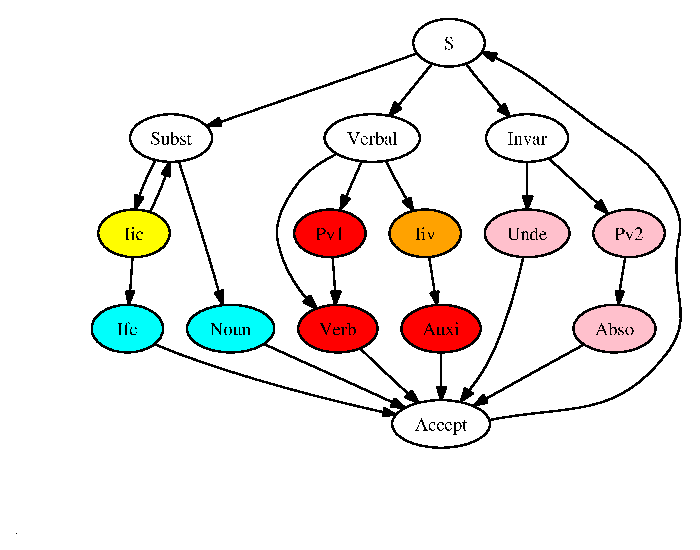
\includegraphics[width=11cm]{skt} \end{center} % comment-out for html

\section{Producing the engine}

We now have all the pieces to connect our dispatch plug-in to the generic reactive
engine, parameterized by the automata vector provided by the user for recognizing the
various phases. Let us give a concrete example. 

Given the {\it automata} functor corresponding to Sanskrit
morphology in a {\it Sanskrit\_dispatch} module, we show how to
link it to the {\it Reactt} functor in order to produce a Sanskrit engine generator: 
\typeout{OcamlWeb file Sanskrit_engine.ml}
\ocwmodule{Sanskrit\_engine}
\label{../sanskrit_engine.ml:0}%
Engine \ocwbegindcode{}$\ocwlowerid{sanskrit\_engine}$\ocwenddcode{} using aumt structure with sanskrit.aut. 
\ocweol
\label{../sanskrit_engine.ml:689}%
\medskip
\ocwbegincode{}\ocwindent{0.00em}
\ocwkw{open}~$\ocwupperid{Aumt};~$\ocwbc{} Auto \ocwec{}\ocweol
\ocwindent{0.00em}
\ocwkw{open}~$\ocwupperid{Reactt};~$\ocwbc{} React \ocwec{}\ocweol
\ocwindent{0.00em}
\ocwkw{open}~$\ocwupperid{Sanskrit\_dispatch};~$\ocwbc{} Automata \ocwec{}\medskip

\label{../sanskrit_engine.ml:776}%
\ocwindent{0.00em}
\ocwkw{module}~$\ocwupperid{Automata\_Aumt}~=~\ocwupperid{Automata}~\ocwupperid{Auto}$\ocweol
\ocwindent{0.00em}
;\ocweol
\ocwindent{0.00em}
\ocwkw{open}~$\ocwupperid{Automata\_Aumt};~$\ocwbc{} \ocwbegindcode{}$\ocwlowerid{auto\_vect}$\ocwenddcode{} Disp \ocwec{}\medskip

\label{../sanskrit_engine.ml:859}%
\ocwindent{0.00em}
\ocwkw{module}~$\ocwupperid{Gen\_engine}$\ocweol
\ocwindent{0.50em}
$(\ocwupperid{Fsm}:~$\ocwkw{sig}~$\ocwlowerid{value}~\ocwlowerid{autos}:~\ocwlowerid{auto\_vect};~$\ocwkw{end}$)~=~$\ocwkw{struct}\medskip

\label{../sanskrit_engine.ml:928}%
\ocwindent{1.00em}
\ocwkw{module}~$\ocwupperid{Phases}~=~\ocwupperid{Disp}~\ocwupperid{Fsm}$\ocweol
\ocwindent{1.00em}
;\ocweol
\ocwindent{1.00em}
\ocwkw{open}~$\ocwupperid{Phases}~$\ocwbc{} phase, transducer, etc \ocwec{}\ocweol
\ocwindent{1.00em}
;\ocweol
\ocwindent{1.00em}
\ocwkw{module}~$\ocwupperid{Engine}~=~\ocwupperid{React}~\ocwupperid{Phases}$\ocweol
\ocwindent{1.00em}
;\ocweol
\ocwindent{0.50em}
\ocwkw{end}\ocweol
\ocwindent{0.00em}
;\medskip

\ocwendcode{}\ocwindent{0.00em}
Now we may provide the Sanskrit lexicons for the various lexical sorts as a vector 
\ocweol
\ocwindent{0.00em}
\ocwbegindcode{}$\ocwlowerid{auto\_vect}=\{\ocwlowerid{epsilon\_aum}=\ocwlowerid{aum\_0};~\ocwlowerid{noun}=\ocwlowerid{aum\_noun};~...~\ocwlowerid{prev}=\ocwlowerid{aum\_prev}\}$\ocwenddcode{} 
\ocweol
\ocwindent{0.00em}
in a module \ocwbegindcode{}$\ocwupperid{Sanskrit\_Aumt}$\ocwenddcode{}. 
\ocweol
\ocwindent{0.00em}
We may then call the properly instanciated functor
\ocwbegindcode{}$(\ocwupperid{Gen\_engine}~\ocwupperid{Sanskrit\_Aumt})$\ocwenddcode{} in order to get e.g. \ocwbegindcode{}$\ocwupperid{Engine}.\ocwlowerid{react1}$\ocwenddcode{}. 
\ocweol

What we just constructed is a simple engine which may recognize a Sanskrit sentence 
as a sequence of inflected word forms. Actually such forms are glued together 
using a euphony junction
process known as {\sl sandhi}. It is possible to invert the sandhi relation while doing
the recognition, and to use the transducer output to give a trace of the sandhi relation
between the words. Piping this process through a lemmatizer, which itselfs inverts the
flexional morphology, yields a Sanskrit tagger. This application is described in
\cite{2004-Huet-1}. 


\begin{thebibliography}{10}

\bibitem{asu} Alfred V. Aho, Ravi Sethi and Jeffrey D. Ullman.
``Compilers - Principles, Techniques and Tools.'' Addison-Wesley, 1986.

\bibitem{beeskar} Kenneth R. Beesley and Lauri Karttunen. ``Finite-State 
Morphology: Xerox Tools and Techniques.'' Private communication, April 2001.

\bibitem{bentley} Jon L. Bentley and Robert Sedgewick.
``Fast Algorithms for Sorting and Searching Strings.'' 
Proceedings, 8th Annual ACM-SIAM Symposium on Discrete Algorithms, Jan. 1997.

\bibitem{berrysethi}
G\'erard Berry and Ravi Sethi.
From regular expressions to deterministic automata.
Theoretical Computer Science 48 (1986), pp. 117--126.

\bibitem{berstelpin}
Jean Berstel and Jean-Eric Pin. Local languages and the {Berry}-{Sethi} algorithm.
Theoretical Computer Science 155 (1996), pp. 439--446.

\bibitem{brill} Eric Brill. ``A simple rule-based part of speech tagger.''
In Proceedings, Third Conference on Applied Natural Language Processing, 1992.
Trento, Italy, 152--155. 

\bibitem{burge} W. H. Burge. ``Recursive Programming Techniques.''
Addison-Wesley, 1975. 

\bibitem{fp} Guy Cousineau and Michel Mauny. ``The Functional Approach to
Programming.'' Cambridge University Press, 1998.

\bibitem{daciuk} Jan Daciuk, Stoyan Mihov, Bruce W. Watson and Richard E. 
Watson. ``Incremental Construction of Minimal Acyclic Finite-State Automata.''
Computational Linguistics 26,1 (2000). 

\bibitem{eilenberg}
Samuel Eilenberg. Automata, Languages, and Machines, volume A.
Academic Press, 1974.

\bibitem{MLer} Matthias Felleisen and Daniel P. Friedman. ``The Little MLer''. 
MIT Press, 1998.

\bibitem{flajsipste} Philippe Flajolet, Paola Sipala and Jean-Marc Steyaert.
``Analytic Variations on the Common Subexpresssion Problem.'' Proceedings of
17th ICALP  Colloquium, Warwick (1990), LNCS 443, Springer-Verlag,
pp. 220--234.

\bibitem{ML-LCF}
M.  Gordon, R.  Milner, C.  Wadsworth.
``A Metalanguage for Interactive Proof in LCF.''
Internal Report CSR-16-77, Department of Computer Science,
University of Edinburgh (Sept. 1977).

\bibitem{zipper} G\'erard Huet. ``The Zipper''. J. Functional Programming 7,5 
(Sept. 1997), pp. 549--554.

\bibitem{dico-report} 
G\'erard Huet.
``Structure of a Sanskrit dictionary.''
INRIA Technical Report, Sept. 2000.
Available as: \raggedright
\verb!http://pauillac.inria.fr/~huet/PUBLIC/Dicostruct.ps!.

\bibitem{wcre}
G\'erard Huet.
``From an informal textual lexicon to a well-structured lexical database:
An experiment in data reverse engineering.''
IEEE Working Conference on Reverse Engineering (WCRE'2001), 
Stuttgart, Oct. 2001.

\bibitem{2003-Huet-3} 
G\'erard Huet. Automata Mista. In ``Verification: Theory and Practice: Essays Dedicated
to {Zohar} {Manna} on the Occasion of His 64th Birthday". Ed. Nachum Dershowitz,
Springer-Verlag LNCS vol. 2772 (2004), pp. 359--372.

\bibitem{2004-Huet-1}
G\'erard Huet. A Functional Toolkit for Morphological
and Phonological Processing, Application to a {Sanskrit} Tagger.
J. Functional Programming, 15,4 (2005), pp. 573--614. 

\bibitem{2006-Huet-Razet}
G\'erard Huet and Beno{\^\i}t Razet. The Reactive Engine for Modular Transducers.
In ``Algebra, Meaning and Computation, Essays Dedicated to 
Joseph A. Goguen on the Occasion of His 65th Birthday'', Eds.
Kokichi Futatsugi, Jean-Pierre Jouannaud and Jos\'e Meseguer.
Springer-Verlag LNCS vol. 4060 (2006), pp. 355--374

\bibitem{2008-Huet-Razet}
G\'erard Huet and Beno{\^\i}t Razet. Computing with Relational Machines.
ICON'2008 tutorial. Preliminary version available at URL
\url{http://yquem.inria.fr/~huet/PUBLIC/Pune_tutorial.pdf}.

\bibitem{kk} Ronald M. Kaplan and Martin Kay. ``Regular Models of
Phonological Rule Systems.'' Computational Linguistics (20,3), 1994,
pp. 331--378. 

\bibitem{karttunen1} Lauri Karttunen. ``Applications of Finite-State 
Transducers in Natural Language Processing.'' 
In Proceedings of CIAA-2000.

\bibitem{karttunen2} Lauri Karttunen. ``The Replace Operator.'' 
In Proceedings of ACL'95, Cambridge, MA, 1995. Extended version
in \cite{rs2}.

\bibitem{kosk} K. Koskenniemi. ``A general computational model for word-form
recognition and production.'' In Proceedings, 10th International Conference 
on Computational Linguistics, Stanford (1984). 

\bibitem{laporte} Eric Laporte. 
``Rational Transductions for Phonetic Conversion and Phonology.'' 
Report IGM 96-14, Institut Gaspard Monge, 
Universit\'e de Marne-la-Vall\'ee, Aug. 1995. Also in \cite{rs2}.

\bibitem{ocaml} Xavier Leroy et al. ``Objective Caml.'' See: \raggedright
\verb!http://caml.inria.fr/ocaml/index.html!.

\bibitem{mohri} Mehryar Mohri. ``Finite-State Transducers in Language and 
Speech Processing.'' Computational Linguistics 23,2 (1997), pp. 269--311.

\bibitem{paulson} Larry C. Paulson. ``ML for the Working Programmer.''
Cambridge University Press, 1991.

\bibitem{ranta} Aarne Ranta. ``The GF Language: Syntax and Type System.''
See: \raggedright \verb!http://www.cs.chalmers.se/~aarne/GF/!.

\bibitem{camlp4} Daniel de Rauglaudre. ``The Camlp4 preprocessor."
See: \raggedright \verb!http://caml.inria.fr/camlp4/!.

\bibitem{razet05}
Beno{\^\i}t Razet. Automates modulaires. M\'emoire de Master, 
Universit\'e {Denis} {Diderot} (Paris 7), 2005.

\bibitem{Razet08a}
Beno{\^\i}t Razet. Finite {Eilenberg} Machines.
Proceedings of CIIA 2008, 
Eds. O.H. Ibarra and B. Ravikumar,
Springer-Verlag LNCS vol. 5148 (2008), pp. 242--251.

\bibitem{Razet08b}
Beno{\^\i}t Razet. 
Simulating Finite {Eilenberg} Machines with a Reactive Engine.
In Proceedings of MSFP 2008,
Electric Notes in Theoretical Computer Science,
\url!http://gallium.inria.fr/~razet/PDF/razet_msfp08.pdf!.

\bibitem{Razet09}
Beno{\^\i}t Razet.
Machines d'{Eilenberg} Effectives. Th\`ese de Doctorat,
Universit\'e {Denis} {Diderot} (Paris 7), 2009.

\bibitem{revuz} Dominique Revuz. ``Dictionnaires et lexiques.'' Th\`ese de
Doctorat, Universit\'e Paris VII, Feb. 1991.

\bibitem{rs1} Emmanuel Roche and Yves Schabes. ``Deterministic Part-of-Speech
Tagging with Finite-State Transducers.'' 
Computational Linguistics 21,2 (1995), pp. 227-253.

\bibitem{rs2} Emmanuel Roche and Yves Schabes, Eds.
``Finite-State Language Processing.'' MIT Press, 1997.

\bibitem{sproat} Richard Sproat. ``Morphology and Computation."
MIT Press, 1992.

\bibitem{sproatshih} Richard Sproat, Chilin Shih, William Gale and Nancy Chang.
``A Stochastic Finite-State Word-Segmentation Algorithm for Chinese.''
Computational Linguistics 22,3 (1996), pp. 377--408.

\bibitem{caml} Pierre Weis and Xavier Leroy. ``Le langage Caml.'' 
2\`eme \'edition, Dunod, Paris, 1999. 

\end{thebibliography}



\ocwbeginindex{}
\ocwrefindexentry{$\ocwupperid{Ascii}$ (module)}{../ascii.ml:0}{../lexicon.ml:814,../lexicon.ml:951}{\ref{../ascii.ml:0}}{\ref{../lexicon.ml:814}, \ref{../lexicon.ml:951}}
\ocwrefindexentry{$\ocwupperid{Aum0}$ (module)}{../aum0.mli:0}{}{\ref{../aum0.mli:0}}{}
\ocwrefindexentry{$\ocwupperid{Aumt}$ (module)}{../aumt.mli:0}{}{\ref{../aumt.mli:0}}{}
\ocwrefindexentry{$\ocwupperid{Bintree}$ (module)}{../bintree.ml:0}{}{\ref{../bintree.ml:0}}{}
\ocwrefindexentry{$\ocwupperid{Dagify}$ (module)}{../dagify.ml:0}{}{\ref{../dagify.ml:0}}{}
\ocwrefindexentry{$\ocwupperid{Deco}$ (module)}{../deco.ml:0}{}{\ref{../deco.ml:0}}{}
\ocwrefindexentry{$\ocwupperid{Gen}$ (module)}{../gen.ml:0}{}{\ref{../gen.ml:0}}{}
\ocwrefindexentry{$\ocwupperid{Latin}$ (module)}{../latin.ml:0}{}{\ref{../latin.ml:0}}{}
\ocwrefindexentry{$\ocwupperid{Lexicon}$ (module)}{../lexicon.ml:0}{}{\ref{../lexicon.ml:0}}{}
\ocwrefindexentry{$\ocwupperid{Lexmap}$ (module)}{../lexmap.ml:0}{}{\ref{../lexmap.ml:0}}{}
\ocwrefindexentry{$\ocwupperid{List2}$ (module)}{../list2.ml:0}{}{\ref{../list2.ml:0}}{}
\ocwrefindexentry{$\ocwupperid{Make\_english\_lexicon}$ (module)}{../make_english_lexicon.ml:0}{}{\ref{../make_english_lexicon.ml:0}}{}
\ocwrefindexentry{$\ocwupperid{Make\_french\_lexicon}$ (module)}{../make_french_lexicon.ml:0}{}{\ref{../make_french_lexicon.ml:0}}{}
\ocwrefindexentry{$\ocwupperid{Make\_lex}$ (module)}{../make_lex.ml:0}{}{\ref{../make_lex.ml:0}}{}
\ocwrefindexentry{$\ocwupperid{Mini}$ (module)}{../mini.ml:0}{}{\ref{../mini.ml:0}}{}
\ocwrefindexentry{$\ocwupperid{Minimap}$ (module)}{../minimap.mli:0,../minimap.ml:0}{}{\ref{../minimap.mli:0}, \ref{../minimap.ml:0}}{}
\ocwrefindexentry{$\ocwupperid{Minitertree}$ (module)}{../minitertree.ml:0}{}{\ref{../minitertree.ml:0}}{}
\ocwrefindexentry{$\ocwupperid{Pidgin}$ (module)}{../pidgin.ml:0}{}{\ref{../pidgin.ml:0}}{}
\ocwrefindexentry{$\ocwupperid{React0}$ (module)}{../react0.ml:0}{}{\ref{../react0.ml:0}}{}
\ocwrefindexentry{$\ocwupperid{Reactt}$ (module)}{../reactt.ml:0}{}{\ref{../reactt.ml:0}}{}
\ocwrefindexentry{$\ocwupperid{Regular}$ (module)}{../regular.ml:0}{}{\ref{../regular.ml:0}}{}
\ocwrefindexentry{$\ocwupperid{Sanskrit\_engine}$ (module)}{../sanskrit_engine.ml:0}{}{\ref{../sanskrit_engine.ml:0}}{}
\ocwrefindexentry{$\ocwupperid{Share}$ (module)}{../share.mli:0,../share.ml:0}{}{\ref{../share.mli:0}, \ref{../share.ml:0}}{}
\ocwrefindexentry{$\ocwupperid{Tertree}$ (module)}{../tertree.ml:0}{}{\ref{../tertree.ml:0}}{}
\ocwrefindexentry{$\ocwupperid{Transducer}$ (module)}{../transducer.ml:0}{}{\ref{../transducer.ml:0}}{}
\ocwrefindexentry{$\ocwupperid{Trie}$ (module)}{../trie.ml:0}{../lexicon.ml:814,../lexicon.ml:951}{\ref{../trie.ml:0}}{\ref{../lexicon.ml:814}, \ref{../lexicon.ml:951}}
\ocwrefindexentry{$\ocwupperid{Unglue}$ (module)}{../unglue.ml:0}{}{\ref{../unglue.ml:0}}{}
\ocwrefindexentry{$\ocwupperid{Unglue\_test}$ (module)}{../unglue_test.ml:0}{}{\ref{../unglue_test.ml:0}}{}
\ocwrefindexentry{$\ocwupperid{Word}$ (module)}{../word.ml:0}{}{\ref{../word.ml:0}}{}
\ocwrefindexentry{$\ocwupperid{Zen\_lexer}$ (module)}{../zen_lexer.ml:0}{}{\ref{../zen_lexer.ml:0}}{}
\ocwrefindexentry{$\ocwupperid{Zipper}$ (module)}{../zipper.ml:0}{}{\ref{../zipper.ml:0}}{}


\ocwendindex{}
\end{document}
